\documentclass[a4paper]{article}
%\usepackage[top=30pt,left=30pt,right=30pt]{geometry}
\usepackage[german,english]{babel}
%\usepackage[utf8]{inputenc}
\usepackage{amsmath}
\usepackage{amssymb}
\usepackage{amsthm}
\usepackage{graphicx}
\usepackage{caption}
\usepackage{fontspec}
\usepackage{mdframed}
\usepackage{pxfonts}
\usepackage{wasysym}
\usepackage{framed}
\usepackage{xcolor}
\usepackage{makeidx}
\usepackage{csquotes}
\usepackage[pdfborder={0 0 0}]{hyperref}
\usepackage{stmaryrd}
\usepackage{titlesec}
\titleformat{\paragraph}{\normalfont\itshape}{}{}{}

\setmainfont{Alegreya}[
  Path = /home/meisterluk/.fonts/alegreya/ ,
  UprightFont = {Alegreya-Regular-with-doublearrow.otf} ,
  BoldFont = {Alegreya-Bold.otf} ,
  ItalicFont = {Alegreya-Italic.otf} ,
  BoldItalicFont = {Alegreya-BoldItalic.otf} ,
]

\newcounter{lecref}[section]
\numberwithin{lecref}{section}

\newtheorem{theorem}[lecref]{Theorem} 
\newtheorem*{Theorem}{Theorem}
\newtheorem{example}[lecref]{Example}
\newtheorem*{Example}{Example}
\newtheorem{definition}[lecref]{Definition}
\newtheorem*{Definition}{Definition}
\newtheorem{lemma}[lecref]{Lemma}
\newtheorem*{Lemma}{Lemma}
\newtheorem*{claim}{Claim}
\newtheorem{remark}[lecref]{Remark}
\newtheorem*{Remark}{Remark}
\newtheorem{corollary}[lecref]{Corollary}
\newtheorem{proposition}[lecref]{Proposition}
\newtheorem*{Person}{Person}
\newtheorem{problem}[lecref]{Problem}
\newtheorem*{hypothesis}{Hypothesis}

% definitions
\newcommand{\drawing}[1]{%
 \begin{figure}[t]
  \begin{center}
   \includegraphics{#1}
  \end{center}
 \end{figure}
}
\newcommand{\pic}[2]{%
 \begin{figure}[t]
  \begin{center}
   \includegraphics{#1}
   \caption{#2}
  \end{center}
 \end{figure}
}
\newcommand{\set}[1]{\left\{#1\right\}}
\newcommand{\setdef}[2]{\left\{\left.#1\,\right|\,#2\right\}}
\newcommand{\ip}[2]{\left\langle#1,#2\right\rangle} % inner product
\newcommand{\angel}[1]{\left\langle#1\right\rangle}
\newcommand{\norm}[1]{\left\|#1\right\|}
\newcommand{\card}[1]{\left|#1\right|}
\newcommand{\given}[1]{\textbf{Given.} #1\par}
\newcommand{\find}[1]{\textbf{Find.} #1\par}
\newcommand{\dateref}[1]{%
  \begin{mdframed}[backgroundcolor=gray!10,innerbottommargin=0pt,innertopmargin=0pt]
    \paragraph{\textit{$\downarrow$ This lecture took place on #1.}}%
  \end{mdframed}%
}
\newcommand{\exist}{\;\exists\,}
\newcommand{\fall}{\;\forall\,}
\newcommand{\noproof}[1]{A proof for Theorem~\ref{#1} is not provided.}
\newcommand{\vectwo}[2]{\begin{pmatrix} #1 \\ #2 \end{pmatrix}}
\newcommand{\vecthree}[3]{\begin{pmatrix} #1 \\ #2 \\ #3 \end{pmatrix}}
\makeatletter
\newcommand{\xRightarrow}[2][]{\ext@arrow 0359\Rightarrowfill@{#1}{#2}}
\makeatother
\newcommand{\rh}[1]{\vec{#1}}
\newcommand{\sout}[1]{#1} % TODO define a strike-through for math mode
\newcommand{\mtn}{(\mu\times\nu)} % mu times nu
\newcommand{\divides}{\,\big|\,} % mu times nu
\def\braket#1{\mathinner{\langle{#1}\rangle}}

\DeclareMathOperator{\rank}{rank}
\DeclareMathOperator{\diag}{diag}
\DeclareMathOperator{\detm}{det}
\DeclareMathOperator{\perm}{perm}
\DeclareMathOperator{\sign}{sign}
\DeclareMathOperator{\degree}{deg}
\DeclareMathOperator{\im}{im}
\DeclareMathOperator{\ke}{kern}
\DeclareMathOperator{\prop}{probability}
\DeclareMathOperator{\Hom}{Hom}
\DeclareMathOperator{\argmax}{argmax}
\DeclareMathOperator{\argmin}{argmin}
\DeclareMathOperator{\vol}{vol}  % volume
\DeclareMathOperator*{\bigtimes}{\vartimes}

\makeatletter
\providecommand*{\dotcup}{%
  \mathbin{%
    \mathpalette\@dotcup{}%
  }%
}
\newcommand*{\@dotcup}[2]{%
  \ooalign{%
    $\m@th#1\cup$\cr
    \hidewidth$\m@th#1\cdot$\hidewidth
  }%
}
\makeatother


% metadata
\title{
  Linear Algebra 2 \\
  \large{Lecture notes, University (of Technology) Graz} \\
  based on the lecture by Franz Lehner
}
\date{\today}
\author{Lukas Prokop}

% settings
\parindent0pt
\setlength{\parskip}{0.4\baselineskip}

\setcounter{section}{5}
\makeindex

\begin{document}
\maketitle
\tableofcontents

\section{Preface}
\dateref{2018/03/05}

\subsection{Lecture}

\begin{itemize}
  \item Mon, 08:15--09:45, lecture
  \item Wed, 08:15--09:45, lecture
  \item Mon, 16:00--18:00, tutorial, AE01
  \item Mon, 13:15--14:00, conversatorium (BE01)
\end{itemize}

\subsection{Linear algebra 1}

\begin{Person}
  Gottfried Wilhelm von Leibniz (1646--1716)
\end{Person}
Results from 1693:
\begin{itemize}
  \item Vector spaces (first definition in 1880)
  \item Matrices and linear maps
\end{itemize}
From now, it will be more specific ($\rightarrow$ matrices).
In general, we discuss the question \enquote{when is a matrix invertible}?
\begin{align*}
  ax + by &= e \\
  cx + dy &= f
\end{align*}
We need to invert the matrix.

Assuming $a \neq 0$. We multiply the first row with $\cdot \frac1a \cdot (-c)$.
\[
  \begin{array}{cc|cc}
    a & b & 1 & 0 \\
    c & d & 0 & 1 \\
  \hline
    0 & d-\frac ca \cdot b & -\frac ca & 1
  \end{array}
\]
We then divide by $d - \frac ca b$ if $\neq 0$.

If $a=0$ and $c=0$, rank is certainly not $2$.

If $a=0$ and $c \neq 0$, we multiply with $\frac1c (-a)$.
\[
  \begin{array}{cc}
    a & b \\
    c & d \\
  \hline
    0 & b-\frac{ad}{c}
  \end{array}
\]
we divide $b - \frac{ad}{c}$ if $\neq 0$.

When does such a system have a non-trivial solution?
There is a non-trivial solution iff $ad - bc \neq 0$.

$ad - bc \neq 0$ iff $\begin{pmatrix} a & b \\ c & d \end{pmatrix}$ is invertible.

Leibniz was not the first discovering it. The result was found before 1685 by Sehi Takahazu.

\section{Determinants}

\subsection{Definition}

\index{Determinant of a matrix}
\begin{definition} % Definition 7.1
  \[ \det{\begin{pmatrix} a & b \\ c & d \end{pmatrix}} \eqqcolon ad - bc \eqqcolon \begin{vmatrix} a & b \\ c & d \end{vmatrix} \]
  is called \emph{determinant of matrix $\begin{pmatrix} a & b \\ c & d \end{pmatrix}$}.
\end{definition}

\subsection{Properties}

\begin{Remark} \hfill{}
  \begin{itemize}
    \item The determinant is linear in every row and every column.
      For fixed $b$ and $d$, it is
      \[ \vectwo xy \mapsto \det{\begin{pmatrix} x & b \\ y & d \end{pmatrix}} = dx - by \qquad \text{ is linear} \]
      \[ \mathbb K^2 \to \mathbb K \]
      \begin{align*}
        \det{\begin{pmatrix} \lambda x + \mu x' & b \\ \lambda y + \mu y' & d \end{pmatrix}}
          &= d \cdot (\lambda x + \mu x') - b \cdot (\lambda y + \mu y') \\
          &= \lambda (dx - by) + \mu (dx' - by') \\
          &= \lambda \det{\begin{pmatrix} x & b \\ y & d \end{pmatrix}} + \mu \det{\begin{pmatrix} x' & b \\  y' & d \end{pmatrix}}
      \end{align*}
      The determinant is bilinear in rows and columns.
      \[ \det(\lambda \nu + \mu \nu', w) = \lambda \det(\nu, w) + \mu \det(\nu', w) \]
      Let $\nu = \vectwo{a}{c}$.
      \[ \det(\nu, \lambda w + \mu w') = \lambda \det(\nu, w) + \mu \det(\nu, w') \]
      Let $w = \vectwo bd$.
      Follows analogously.
    \item If two rows are the same, then $\det(M) = 0$.
      \[ \det\begin{pmatrix} a & b \\ c & d \end{pmatrix} = ab - ba = 0 \]
      \[ \det\begin{pmatrix} a & a \\ c & c \end{pmatrix} = ac - ca = 0 \]
    \item The determinant of the unit matrix is one.
      \[ \det\begin{pmatrix} 1 & 0 \\ 0 & 1 \end{pmatrix} = 1 \]
  \end{itemize}
\end{Remark}

\index{Bilinearity}
\begin{theorem}[properties 1--3 characterize the determinant] % section 7.3
  If $\varphi: \mathbb K^2 \times \mathbb K^2 \to \mathbb K$ and $\varphi$ satisfies the properties 1--3,
  $\varphi$ is the determinant.
  \begin{description}
    \item[bilinear\footnote{Bilinear means linear in both components}]
      \[ \varphi(\lambda v + \mu v', w) = \lambda \varphi(v, w) + \mu \varphi(v', w) \]
      \[ \forall v,w,v',w': \mu(v, \lambda w + \mu w') = \lambda \varphi(v, w) + \mu \varphi(v, w') \]
    \item \[ \forall \nu: \varphi(\nu, v) = 0 \]
      \[ \implies \varphi = \det{} \]
    \item $\varphi(e_1, e_2) = 1$
  \end{description}
\end{theorem}

\begin{proof}
  \[ v = \begin{pmatrix} a \\ c \end{pmatrix} = a \cdot e_1 + c \cdot e_2 \]
  \[ w = \vectwo db = b \cdot e_1 + d \cdot e_2 \]
  \begin{align*}
    \varphi(v, w) &= \varphi(a \cdot e_1 + c \cdot e_2, b \cdot e_1 + d \cdot e_2) \\
      &= a \cdot \varphi(e_1, b \cdot e_1 + d \cdot e_2) + c \cdot \varphi(e_2, b \cdot e_1 + d \cdot e_2) \\
      &= a b \cdot \underbrace{\varphi(e_1, e_1)}_{=0} + ad \cdot \varphi(e_1, e_2) + cb \cdot \varphi(e_2, e_1) + cd \cdot \underbrace{\varphi(e_2, e_2)}_{=0} \\
    \intertext{Is zero, because of property~3.}
      &= ad \cdot \underbrace{\varphi(e_1, e_2)}_{=1} + cb \cdot \varphi(e_2, e_1)
  \end{align*}
  \[ 0 = \varphi(e_1 + e_2, e_1 + e_2) = \underbrace{\varphi(e_1, e_1)}_{=0} + \underbrace{\varphi(e_1, e_2)}_{=1} + \varphi(e_2, e_1) + \underbrace{\varphi(e_2, e_2)}_{=0} \]
  \[ \implies \varphi(e_2, e_2) = -1 \]
\end{proof}

\begin{corollary} % section 7.4
  \[ \forall v, w: \varphi(v, w) = -\varphi(w, v) \]
\end{corollary}

\begin{figure}[t]
  \begin{center}
    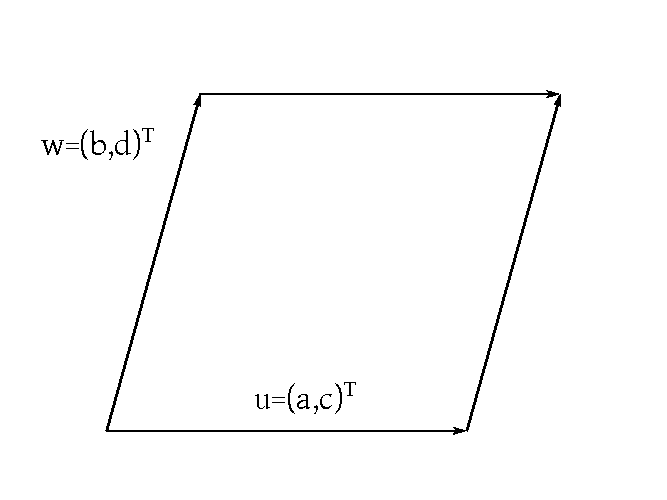
\includegraphics{img/01_geometric_interpretation_determinant.pdf}
    \caption{Geometric interpretation of determinants}
    \label{img:geo_det}
  \end{center}
\end{figure}

\begin{corollary}[Geometrical interpretation]
  See Figure~\ref{img:geo_det}.
  The determinant $\det(v,w)$ is the area of the spanned parallelogram.
  We denote $F$ as the function returning the area of a geometric object.
\end{corollary}

\begin{proof}
  $\operatorname{area}(v,w)$ satisfies properties $(i)-(iii)$.

  Consider orthogonal $e_1$ and $e_2$.
  $F = 1 = \det(e_1, e_2)$. $\det(e_2, e_1) = -1$.

  The sign indicates the orientation of the area.
\end{proof}

By property~2, if $v=w$, then $F = 0$.
\index{Linear dependence}
By property~1,
\begin{enumerate} % 7.5
  \item 
    If $v$ and $w$ are \emph{linear dependent}\footnote{Hence, one vector is a multiple of the other}, then
    \[ \lambda v + \mu w = 0 \qquad (\lambda, \mu) \neq (0, 0) \]
    Without loss of generality, $\mu \neq 0 \implies w = - \frac{\lambda}{\mu} \cdot v$.
  \item
    To show:
    \[ F(\lambda v, w) = \lambda \cdot F(v, w) \]
    \[ F(v + v', w) = F(v, w) + F(v', w) \]

    Let $\lambda \in \mathbb N$. We multiply the area $n$ times.
    \[ F(n \cdot v, w) = n \cdot F(v, w) \]
  \item
    \[ F\left(\frac1n \cdot v, w\right) = \frac1n F(v, w) \]
    follows from $F(\lambda v, w) = \lambda \cdot F(v, w)$, because $v = n \cdot \left(\frac1n v\right)$:
    \[ F\left(n \left(\frac1n v\right), w\right) = n \cdot F\left(\frac1n v, w\right) \]
  \item
    \begin{figure}[!ht]
      \begin{center}
        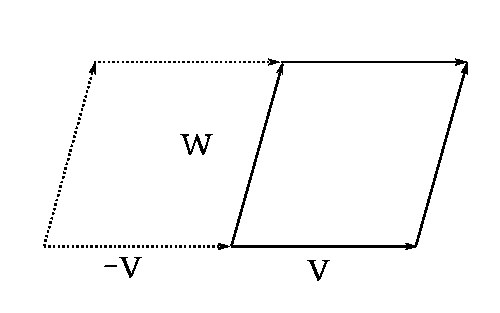
\includegraphics{img/02_continuity.pdf}
        \caption{The sign changes if the orientation changes}
        \label{img:continuity}
      \end{center}
    \end{figure}
    If we combine (2) and (3),
    \[ F\left(\frac mn v, w\right) = \frac mn F(v, w) \]
    See Figure~\ref{img:continuity}.
  \item
    By continuity, $F(\lambda v, w) = \lambda F(v, w) \forall \lambda \in \mathbb R_+$\footnote{By the way, how are real numbers defined?}.
    If the orientation changes, the sign changes. By this property, this actually holds for $\mathbb R$, not only $\mathbb R_+$.

    Analogously:
    \[ F(v, \lambda w) = \lambda F(v, w) \forall \lambda \in \mathbb R \forall v, w \in \mathbb R^2 \]
  \item
    To show: $F(v + v', w) = F(v, w) + F(v', w)$

    If $v$ and $w$ are linear independent, then $F(v + w, w) = F(v, w)$.
    In general, for a parallelogram of height $h$ and vector $w$, it holds that
    \[ F = \card{w} \cdot h \]
    The height of the parallelogram stays the same.
    \[ F(v, w) = F(v + w, w) \]
  \item 
    \[ F(\lambda v + \mu w, w) = \lambda F(v, w) \]
    \begin{description}
      \item[Case $\mu = 0$] Already shown, $F(\lambda v, w) = \lambda F(v, w) \forall \lambda \in \mathbb R$.
      \item[Case $\mu \neq 0$] $F(\lambda v + \mu w, w) = \frac1\mu F(\lambda v + \mu w, \mu w) = \frac1\mu F(\lambda v, \mu w) = F(\lambda v, w) = \lambda F(v, w)$
    \end{description}
  \item
    Let $v$ and $w$ be linear independent, then they define a basis of $\mathbb R^2$.
    \begin{align*}
      v_1 &= \lambda_1 v + \mu_1 w \\
      v_2 &= \lambda_2 v + \mu_2 w
    \end{align*}
    \begin{align*}
      \rightarrow F(v_1 + v_2, w)
        &= F(\lambda_1 v + \mu, w + \lambda_2 v + \mu_2 w, w) \\
        &= F((\lambda_1 + \lambda_2) v + (\mu_1 + \mu_2) w, w) \\
        &= F((\lambda_1 + \lambda_2) v, w) \\
        &= (\lambda_1 + \lambda_2) F(v, w) \\
        &= \lambda_1 F(v,w) + \lambda_2 F(v,w) \\
        &= F(\lambda_1 v, w) + F(\lambda_2 v, w) \\
        &= F(\lambda_1 v + \mu_1 w, w) + F(\lambda_2 v + \mu_2 w, w) \\
        &= F(v_1, w) + F(v_2, w)
    \end{align*}
    This shows that additivity is given.
\end{enumerate}

\subsection{Determinant form} % section 7.6

\begin{definition}
  \index{Determinant form}
  Let $V$ be an $n$-dimensional vector space over $\mathbb K$.
  A \emph{determinant form} is a map
  \[ \triangle: V^n \to \mathbb K \]
  \[ (a_1, \ldots, a_n) \mapsto \triangle (a_1, \ldots, a_n) \]
\end{definition}
Let $n=2$.
\[ \triangle: \left(\vectwo ac, \vectwo bd\right) \mapsto \begin{vmatrix} a & b \\ c & d \end{vmatrix} = ad - bc \]

\index{Multilinearity}
It satisfies the properties of \emph{multilinearity}:
\begin{enumerate}
  \item $\triangle(a_1, \dots, \lambda a_k, \dots, a_n) = \lambda \triangle(a_1, \dots, a_n)$
  \item $\triangle(a_1, \dots, a_k + v, \dots, a_n) = \triangle(a_1, \dots, a_k, \dots, a_n) + \triangle(a_1, \dots, a_{k-1}, v, a_{k+1}, \dots, a_n)$
\end{enumerate}
Multilinearity is given, if linearity is given in every component.
Hence, if $a_1, \dots, a_{k-1}, a_{k+1}, \dots, a_n$ are fixed, then
\[ V \to \mathbb K \]
\[ v \mapsto \triangle (a_1, \dots, a_{k-1}, v, a_{k+1}, \dots, a_n) \text{ linear} \]

Furthermore, it satisfies the following property:
\begin{enumerate}
  \item[3.] $\triangle(a_1, \dots, a_n) = 0$ \\
    if $\exists k \neq l: a_k = a_l$.
    If $\triangle \not\equiv 0$, then $\triangle$ is called \emph{non-trivial}.
\end{enumerate}

\begin{corollary} % section 7.7
  \begin{enumerate}
    \item[4.]
      $\triangle(a_1, \dots, a_k + \lambda a_i, \dots, a_n) = \triangle(a_1, \dots, a_k, \dots, a_n) \forall \lambda \in \mathbb K, \forall i \neq k$
    \item[5.]
      $\triangle(a_1, \dots, a_i, \dots, a_j, \dots, a_n) = -\triangle(a_1, \dots, a_j, \dots, a_i, \dots, a_n)$
  \end{enumerate}
\end{corollary}
\begin{proof}
  \begin{enumerate}
    \item[4.]
      \begin{align*}
        \triangle(a_1, \dots, a_k + \lambda a_i, \dots, a_n)
          &= \triangle (a_1, \dots, a_k, \dots, a_n) + \triangle (a_1, \dots, a_{k-1}, \lambda a_i, a_{k+1}, \dots, a_n) \\
          &= \triangle (a_1, \dots, a_n) + \underbrace{\lambda \triangle (a_1, \dots, a_{k-1}, a_i, a_{k+1}, \dots, a_n)}_{= 0 \qquad \text{because $a_i$ occurs twice}}
      \end{align*}
    \item[5.]
      \begin{align*}
        0 &= \triangle(a_1, \dots, a_i + a_j, \dots, a_i + a_j, \dots, a_n) \\
          &= \triangle(a_1, \dots, a_i, \dots, a_i, \dots, a_n) \\
          &+ \triangle(a_1, \dots, a_i, \dots, a_j, \dots, a_n) \\
          &+ \triangle(a_1, \dots, a_j, \dots, a_i, \dots, a_n) \\
          &+ \triangle(a_1, \dots, a_j, \dots, a_j, \dots, a_n)
      \end{align*}
      The first and last summands are zero. Multilinearity is given:
      \[ \lambda(a_1, \dots, \lambda a_k, \dots, a_n) = \lambda \triangle (a_1, \dots, a_n) \]
      \[ \lambda(a_1, \dots, \lambda a_k + v, \dots, a_n) = \lambda \triangle (a_1, \dots, a_n) + \triangle (a_1, \dots, a_{k-1}, v, a_{k+1}, \dots, a_n) \]
  \end{enumerate}
\end{proof}

\dateref{2018/03/07}

Determinant form: $\dim{V} = n$
\[ \triangle: V^n \to \mathbb K \]

\begin{enumerate}
  \item $\triangle(a_1, \dots, a_{k-1}, \lambda a_k, a_{k+1}, \ldots, a_n) = \lambda \triangle(a_1, \dots, a_n)$
  \item $\triangle(a_1, \dots, a_{k-1}, a_k + v, a_{k+1}, \dots, a_n = \triangle(a_1, \dots, a_k, \dots, a_n) + \triangle(a_1, \dots, v, \dots, a_n)$
  \item $\triangle(a_1, \dots, a_n) = 0$ if $\exists i \neq j: a_i = a_j$
\end{enumerate}
Multilinearity is given by the first two properties.

$\triangle \not\equiv 0$

Then the fourth property follows:
\begin{enumerate}
  \item[4.] $\triangle(a_1, \dots, a_{k} + \lambda a_i, \dots, a_n) = \triangle(a_1, \dots, a_n) \forall i \neq k \forall \lambda \in \mathbb K$
  \item[5.] $\triangle(a_1, \dots, a_i, \dots, a_j, \dots, a_n) = -\triangle(a_1, \dots, a_j, \dots, a_i, \dots, a_n)$
\end{enumerate}

\begin{Example}
  Let $n=2$, $V = \mathbb K^2$.

  \[ \triangle \left(\vectwo ac, \vectwo bd\right) = ad - bc = \det\begin{pmatrix} a & b \\ c & d \end{pmatrix} \]
\end{Example}

\subsection{Permutations and transpositions}

\begin{definition} % 7.8
  A \emph{permutation} is a bijective map $\sigma: \set{1,\dots,n} \to \set{1,\dots,n}$.
  $\sigma_n$ is the set of all permutations.
  \[ \card{\sigma_n} = n! \]
\end{definition}

\index{Symmetric group}
\begin{remark} % 7.9
  $\sigma_n$ in regards of composition defines a group with neutral element $\operatorname{id}$
  and is called \emph{symmetric group}.
\end{remark}

\begin{remark} % 7.10
  For $n \geq 3$, it is non-commutative.
\end{remark}

\begin{example} % 7.11
  Permutations:
  \[ \begin{pmatrix} 1 & 2 & 3 & 4 \\ 4 & 1 & 3 & 2 \end{pmatrix} \circ \begin{pmatrix} 1 & 2 & 3 & 4 \\ 1 & 3 & 4 & 2 \end{pmatrix} = \begin{pmatrix} 1 & 2 & 3 & 4 \\ 4 & 3 & 2 & 1 \end{pmatrix} \]
  So, e.g. 2 is mapped to 3 (right side of $\circ$) and 3 is mapped to 3 (left side of $\circ$). Hence 2 is mapped to 3 (right-hand side of $=$).
  \[ \begin{pmatrix} 1 & 2 & 3 & 4 \\ 4 & 1 & 3 & 2 \end{pmatrix}^{-1} = \begin{pmatrix} 1 & 2 & 3 & 4 \\ 2 & 4 & 3 & 1 \end{pmatrix} \]
\end{example}

\begin{definition}
  A \emph{transposition} is a permutation exchanging exactly 2 elements.

  \[
    \tau_{ij} : \begin{cases}
      i \mapsto j \\
      j \mapsto i \\
      k \mapsto k \forall k \notin \set{i,j}
    \end{cases}
  \] \[
    \tau_{ij}^{-1} = \tau_{ij}
  \]
\end{definition}

\begin{Lemma}
  Every permutation $\sigma \in \sigma_n$ with $\sigma \neq \operatorname{id}$ can be denoted as product of transpositions.
\end{Lemma}

\begin{Example}
  \[ \sigma = \begin{pmatrix} 1 & 2 & 3 & 4 & 5 & 6 & 7 \\ 1 & 3 & 5 & 4 & 7 & 6 & 2 \end{pmatrix} \]
\end{Example}

\begin{proof}
  \[ \sigma = \begin{pmatrix} 1 & 2 & \dots & n \\ \sigma(1) & \sigma(2) & \dots & \sigma(n) \end{pmatrix} \]

  Find transpositions $\tau_1, \dots, \tau_k$ such that $\sigma = \tau_1 \circ \tau_2 \circ \dots \circ \tau_k$.

  If $\sigma = \operatorname{id}$, then $k=0$.

  If $\sigma \neq \operatorname{id}$,
  \[ k_1 \coloneqq \min\setdef{i}{\sigma(i) \neq i} \neq \emptyset \]
  \[ \tau_1 \coloneqq \tau_{k_1 \sigma(k_1)} \]
  \[ \sigma_1 \coloneqq \tau_i \circ \sigma \]
  if $\sigma_i = \operatorname{id}$, then $\tau_1 \circ \sigma = \operatorname{id}$. Then $\sigma = \tau_1^{-1} = \tau_i$.
  \[ k_2 \coloneqq \min\setdef{i}{\sigma_i(i) \neq i} \]
  \[ \tau_2 \coloneqq \tau_{k_2 \sigma_1(k_2)} \]
  \[ \sigma_2 \coloneqq \tau_2 \circ \sigma_1 \]
\end{proof}

\begin{Example}
  Let $k_1 = 2$.
  \[ \tau_1 = \tau_{23} \]
  \begin{align*}
    \sigma_1 &= \tau_{23} \circ \begin{pmatrix} 1 & 2 & 3 & 4 & 5 & 6 & 7 \\ 1 & 3 & 5 & 4 & 7 & 6 & 2 \end{pmatrix} \\
      &= \begin{pmatrix} 1 & 2 & 3 & 4 & 5 & 6 & 7 \\ 1 & 2 & 5 & 4 & 7 & 6 & 3 \end{pmatrix}
  \end{align*}
  $k_2 = 3$.
  \[ \tau_2 = \tau_{35} \]
  \begin{align*}
    \sigma_2 = \tau_2 \circ \sigma_1 &= \begin{pmatrix} 1 & 2 & 3 & 4 & 5 & 6 & 7 \\ 1 & 2 & 3 & 4 & 7 & 6 & 5 \end{pmatrix}
  \end{align*}

  $k_3 = 5$.
  \[ T_3 = T_{57} \]
  \begin{align*}
    \sigma_3 = \tau_3 \circ \sigma_2 &= \begin{pmatrix} 1 & 2 & 3 & 4 & 5 & 6 & 7 \\ 1 & 2 & 3 & 4 & 5 & 6 & 7 \end{pmatrix} \\
      &= \operatorname{id}
  \end{align*}
  \[ \tau_3 \circ \tau_2 \circ \tau_1 \circ \sigma = \operatorname{id} \]
  \[ \implies \tau_2 \circ \tau_1 \circ \sigma = T_3^{-1} \circ \operatorname{id} = \tau_3 \]
  \[ \tau_1 \circ \sigma = \tau_2^{-1} \circ T_3 = \tau_2 \circ \tau_3 \]
  \[ \sigma = \tau_1 \circ \tau_2 \circ \tau_3 \]
  and so on and so forth.

  \[ \tau_k \]
  \[ \sigma_k = \tau_k \circ \tau_{k-1} \circ \dots \circ \tau_{i} \circ \sigma = \operatorname{id} \]
  \[ \implies \sigma = \tau_1 \circ \tau_2 \circ \dots \circ \tau_k \]
\end{Example}

\begin{Remark}
  This decomposition is not unique.
\end{Remark}

\index{Malposition}
\index{Signature of $\pi$}
\begin{definition} % 7.14
  Let $\pi \in \sigma_n$ be a permutation.
  A \emph{malposition} (dt. \foreignlanguage{german}{Fehlstand}) of $\pi$ is a pair $(i,j)$ such that $i < j$ and $\pi(i) > \pi(j)$.
  \[ f_\pi \coloneqq \card{\setdef{(i,j)}{(i,j) \text{ is malposition of } \pi}} \]
  \[ \sign(\pi) \coloneqq (-1)^{f_\pi} \eqqcolon (-1)^\pi \]
  is called \emph{signature of $\pi$}
\end{definition}

\begin{example} % 7.15
  \[ \pi = \begin{pmatrix} 1 & 2 & 3 & 4 & 5 & 6 & 7 \\ 1 & 3 & 5 & 4 & 7 & 6 & 2 \end{pmatrix} \]
  Malpositions:
  \[ \set{(2,7), (3,4), (3,7), (5,6), (5,7), (4,7), (6,7)} \]
  \[ 2 < 7 \]
  \[ \pi(2) - 3 > 2 = \pi(7) \]
  \[ f_\pi = 7 \]
\end{example}

\begin{theorem} % 7.16
  \[ \sign(\pi) = \prod_{\substack{i,j \\ i < j}} \frac{\pi(j) - \pi(i)}{j-i} \]
  \begin{enumerate}
    \item ${n \choose 2}$ factors
    \item for transposition, $\sign\tau = -1$.
  \end{enumerate}
\end{theorem}

\begin{proof}
  \[ \prod_{i<j} \frac{\pi(j) - \pi(i)}{j-i} = \frac{\prod_{i<j} (\pi(j) - \pi(i))}{\prod_{i<j} (j-i)} \]
  $\pi$ is bijective in $\set{1, \dots, n}$.
  Hence, every difference (the expression $j - i$) occurs exactly one time in the enumerator and the denomiator with sign $\pm 1$
  depending on whether $(i,j)$ is a malposition or not (statement 1).
  In other words, the term in the enumerator and denominator cancel out if they are not malpositions.
  \[ \sign(\pi(j) - \pi(i)) = \begin{cases}
    +1 & \pi(j) > \pi(i) \\
    -1 & \pi(j) < \pi(i) \text{ hence malposition}
  \end{cases} \]
  Consider any transposition, let $k$ be the first index with $k \neq \pi(k)$ and let $l$ be the last index with $l \neq \pi(l)$. $(k, k+1), (k, k+2), \dots, (k, l-1)$ are $(l-1-k+1+1)$ malpositions. $(k+1, l), (k+2, l), \dots, (l-1, l)$ are $(l-1 - k+1 + 1)$ malpositions. The sum gives an even number. Additional, we have malposition $(k, l)$, thus an odd number of malpositions is given. Thus $\sign\tau = -1$ (statement 2). 
\end{proof}

\begin{Example}
  \[ \pi = \begin{pmatrix} 1 & 2 & 3 & 4 & 5 & 6 & 7 \\ 1 & 3 & 5 & 4 & 7 & 6 & 2 \end{pmatrix} \]
  Malposition:
  \[ \set{(2,7), (3,4), (3,7), (5,6), (5,7), (4,7), (6,7)} \]
  \[ 2 < 7 \]
  \[ \pi(2) - 3 > 2 = \pi(7) \]
  \[ f_\pi = 7 \]

  \[
    \frac{\prod_{i<j} (\pi(j) - \pi(i))}{\pi_{i<j} (j-i)} = \frac{\prod_{i<j} (j-i) \cdot (-1)^{f_\pi}}{\prod_{i<j} (j-i)} = \sign{\pi}
  \]

  \[ \pi = \begin{pmatrix} 1 & 2 & 3 \\ 3 & 2 & 1 \end{pmatrix} \]
  \begin{align*}
    \prod_{i<j} \frac{\pi(j) - \pi(i)}{j-i}
      &= \frac{\pi(2) - \pi(1)}{2 - 1} \cdot \frac{\pi(3) - \pi(1)}{3-1} \cdot \frac{\pi(3) - \pi(2)}{3-2} \\
      &= \frac{(2-3) \cdot (1-3) \cdot (1 - 2)}{(2-1) (3-1) (3-2)} \\
      &= (-1)^3 = -1
  \end{align*}

  Malpositions:
  \begin{enumerate}
    \item $(1,2)$
    \item $(1,3)$
    \item $(2,3)$
  \end{enumerate}

  Transposition: Let $k < \tau(k)$.
  \[
    \tau = \left\{\begin{array}{ccccccccccc}
      1 & 2 & \ldots & k-1 & k       & k+1 & \ldots & \tau(k) & \tau(k+1) & \ldots & n \\
      1 & 2 & \ldots & k-1 & \tau(k) & k+1 & \ldots & k       & \tau(k+1) & \ldots & n
    \end{array}\right\}
  \]
  Malpositions (denoted $F_\tau$):
  \[
    F_\tau = \begin{cases}
      & (k, k+1), \dots, (k, \tau(k)) \\
      & (k+1, \tau(k)), (k+2, \tau(k)), \dots, (\tau(k)-1, \tau(k))
    \end{cases}
  \]

  Let us count on a specific example:
  \[ \begin{pmatrix}
    1 & 2 & 3 & 4 & 5 & 6 & 7 \\
    1 & 2 & 6 & 4 & 5 & 3 & 7
  \end{pmatrix} \]

  \[
    \begin{cases}
      & (3,4), (3,5), (3,6) \\
      & (4,6), (5,6)
    \end{cases}
  \]

  \[ \card{F_\tau} = (\tau(k) - k) + \left((\tau(k) - 1) - k\right) = 2\tau(k) - 2k - 1 = 2(\tau(k) - k) - 1 \text{ even} \]
\end{Example}

\begin{theorem} % 7.17
  \begin{enumerate}
    \item $\sign(\operatorname{id}) = 1$
    \item $\sign(\pi \circ \sigma) = \sign(\pi) \cdot \sign(\sigma)$ \\
      Hence, $\sign\sigma_n \to \set{\pm 1}$ is a homomorphism.

      $(\set{+1, -1}, \cdot)$ is a group $\stackrel{\sim}{=} (\mathbb Z_2, +)$
      \[ +1 \to [0]_2 \qquad -1 \to [1]_2 \]
    \item $\sign(\pi^{-1}) = \sign(\pi)$
  \end{enumerate}
\end{theorem}

\begin{proof}
  \begin{enumerate}
    \item obvious, because there are no malpositions
    \item
      \begin{align*}
        \sign(\pi \circ \sigma) &= \prod_{i<j} \frac{(\pi \circ \sigma(j) - \pi \circ \sigma(i))}{j-i} \prod_{i<j} \frac{\sigma(j) - \sigma(i)}{\sigma(j) - \sigma(i)}
        \intertext{because of bijectivity}
          &= \underbrace{\prod_{i<j} \frac{\pi(\sigma(j)) - \pi(\sigma(i))}{\sigma(j) - \sigma(i)}}_{\sign\pi} \cdot \underbrace{\prod_{i<j} \frac{\sigma(j) - \sigma(i)}{j - i}}_{\sign\sigma}
      \end{align*}
    \item Homomorphism
      \[ \sign(\pi^{-1} \circ \pi) = 1 \iff \sign(\pi^{-1}) \cdot \sign(\pi) = 1 \iff \sign(\pi^{-1}) = \sign(\pi)^{-1} \]
      %\[ \sign(\pi^{-1}) = \sign(\pi)^{-1} = \sign(\pi) \]
  \end{enumerate}
\end{proof}

\begin{Remark}
  Recall that the kernel of a homomorphism defines a subgroup.
\end{Remark}

\index{Alternating group}
\begin{corollary}
  \begin{enumerate}
    \item If $\pi = \tau_1 \circ \dots \circ \tau_k$ is a product of transpositions, then $\sign(\pi) = (-1)^k$
    \item $\mathfrak a_n = \setdef{\pi \in \sigma_n}{\sign(\pi) = +1} = \operatorname{ker}(\set{\sign: \sigma_n \to \set{\pm 1}})$
      is a subgroup of $\sigma_n$, the so-called \emph{alternating group}
      \[ \card{\mathfrak a_n} = \frac{n!}{2} \]
  \end{enumerate}
\end{corollary}

\begin{corollary} % 7.19
  \label{cor:719}
  \[ \dim V = n \qquad \triangle: V^n \to \mathbb K \qquad \text{ determinant form} \]
  then it holds that $\forall \sigma \in \sigma_n: \triangle(a_{\sigma(1)}, \dots, a_{\sigma(n)}) = \sign(\sigma) \cdot \triangle(a_1, \dots, a_n)$
\end{corollary}

\begin{proof}
  If $\sigma = \tau$ is a transposition, by the fourth property we have:
  \[ \triangle(a_{\tau(1)}, \dots, a_{\tau(n)}) = -\triangle(a_1, \dots, a_n) \implies \sign(\tau) = -1 \]

  The general case: $\sigma = \tau_1 \circ \dots \circ \tau_k$ and let $\sigma = \tau_1 \circ \sigma_1$ and $\sigma_1 = \tau_2 \circ \sigma_2$.
  \begin{align*}
    \triangle(a_{\sigma(1)}, \dots, a_{\sigma(n)}) &= \triangle(a_{\tau_1(\sigma_1(1))}, \dots, a_{\tau_1(\sigma_1(n))}) \\
      &= -\triangle(a_{\sigma_1(1)}, \dots, a_{\sigma_1(n)}) & \text{[one transposition applied]} \\
      &= (-1) \triangle(a_{\sigma_1(1)}, \dots, a_{\sigma_1(n)}) \\
      &= (-1)^2 \triangle(a_{\sigma_2(1)}, \dots, a_{\sigma_2(n)}) & \text{[two transpositions applied]} \\
      &= \dots \\
      &= (-1)^k \triangle (a_1, \dots, a_n) \\
      &= \sign(\sigma) \triangle(a_1, \dots, a_n)
  \end{align*}
\end{proof}

\subsection{Leibniz formula for determinants}

\index{Determinant}
\begin{definition}[Definition with theorem] % 7.20
  \label{thm720}
  Define the determinant of matrix $A$.
  \[ \triangle(a_1, \dots, a_n) = \triangle(b_1, \dots, b_n) \cdot \det{A} \]
  if $a_j = \sum_{i=1}^n a_{ij} b_i$. Hence,
  \[ \begin{pmatrix} a_{1j} \\ a_{2j} \\ \vdots \\ a_{nj} \end{pmatrix} = \Phi_{B}(a_j) \]

  \label{det}
  Let $\dim V = n$. Let $B = (b_1, \dots, b_n)$ be a basis of $V$. $a_1, \dots, a_n \in V$ with coordinates
  \[
    \Phi_B(a_j) = \begin{pmatrix} a_{1j} \\ a_{2j} \\ \vdots \\ a_{nj} \end{pmatrix}
    \qquad
    A \coloneqq \begin{bmatrix} a_{11} & \dots & a_{1n} \\ \vdots &  & \vdots \\ a_{n1} & \dots & a_{nn} \end{bmatrix}
  \]
  Then $\triangle(a_1, \dots, a_n) = \det(A) \cdot \triangle(b_1, \dots, b_n)$
  where
  \[ \det(A) \coloneqq \sum_{\pi \in \sigma_n} \sign(\pi) a_{1\pi(1)} a_{2 \pi(2)} \dots a_{n\pi(n)} \]
  is called \emph{determinant of $A$}

  This formula was discovered by Leibniz.
\end{definition}

\begin{Example}
  Consider $n=2$.
  \[
    \begin{vmatrix}
      a_{11} & a_{12} \\
      a_{21} & a_{22}
    \end{vmatrix} = \underbrace{a_{11} a_{22}}_{\pi = \operatorname{id}} - \underbrace{a_{12} a_{21}}_{\pi = \begin{pmatrix} 1 & 2 \\ 2 & 1 \end{pmatrix}}
  \]
\end{Example}

\begin{proof}
  \[ a_j = \sum_{i=1}^n a_{ij} b_i \]
  \begin{align*}
    \triangle(a_1, \dots, a_n) &= \triangle\left(\sum_{i_1 = 1}^n a_{i_1,1} b_{i_1}, \sum_{i_2 = 1}^n a_{i_2,2} b_{i_2}, \dots, \sum_{i_n = 1}^n a_{i_n, n} b_{i_n}\right) \\
    \intertext{because it is multilinear}
      &= \sum_{i_1 = 1}^n \sum_{i_2=1}^n \dots \sum_{i_n=1}^n a_{i_1,1} a_{i_2,2} \dots a_{i_n,n} \cdot \triangle(b_{i_1}, b_{i_2}, \dots, b_{i_n})
  \end{align*}
  where $\triangle$ is zero if $b_i = b_j$.
  \[ \implies i_1,\dots,i_n \text{ are all different elements in } \set{1,\dots,n} \]
  \[ \implies \text{every element occurs exactly once} \]
  \[ i_1,\dots,i_n \text{ is permutation of } 1,\dots,n \]
  \[ \exists \sigma \in \sigma_n: i_1 = \sigma(1), \dots, i_n = \sigma(n) \]
  \begin{align*}
    &= \sum_{\sigma \in \sigma_n} a_{\sigma(1) 1} a_{\sigma(2) 2} \dots a_{\sigma(n) n} \underbrace{\triangle(b_{\sigma(1)} \dots b_{\sigma(n)})}_{\sign\sigma \cdot \triangle(b_1, \dots, b_n) \text{ because of Corollary~\ref{cor:719}}} \\
    &= \sum_{\pi \in \sigma_n} a_{\pi(1) 1} \dots a_{\pi(n) n} \cdot \sign(\pi) \triangle(b_1, \dots, b_n)
  \end{align*}
\end{proof}

\begin{corollary}
  A determinant form is uniquely defined by the value $\triangle(b_1, \dots, b_n)$ on a basis.
  Especially, $\triangle(b_1, \dots, b_n) \not\equiv 0 \iff \triangle(b_1,\dots,b_n) \neq 0$ [for any basis] $\iff \triangle(b_1,\dots,b_n) \neq 0$ [for every basis].
\end{corollary}

\begin{proof}
  Assume $\triangle(b_1,\dots,b_n) = 0$ for any basis.
  Every other basis can be expressed by $b_1, \dots ,b_n$ and the formula gives $\triangle(a_1, \dots, a_n) = 0 \quad \forall a_1,\dots,a_n$.
\end{proof}

\dateref{2018/03/12}

\begin{theorem} % 7.21
  \[ \triangle \text{ non-trivial } \iff \triangle(b_1, \dots, b_n) \neq 0 \text{ for every basis} \]
\end{theorem}

\begin{theorem} % 7.22
  \label{theorem722}
  Inverse of Definition~\ref{det}. %Theorem~\ref{thm720}.
  Given basis $B = (b_1, \dots, b_n)$.
  \[ \triangle(a_1, \dots, a_n) \coloneqq \det\left[\Phi_B(a_1), \dots, \Phi_B(a_n)\right] \]
  defines a non-trivial determinant form such that $\triangle(b_1, \dots, b_n) = 1$.
  % Thus the determinant of every basis is $1$.
\end{theorem}

\begin{Example}
  Let $a_1 = \vectwo46$ and $a_2 = \vectwo{12}{10}$ with $A = (a_1, a_2)$.
  Let $b_1 = \vectwo20$ and $b_2 = \vectwo02$ with $B = (b_1, b_2)$.
  So $\Phi_B(A) = \begin{pmatrix} 2 & 6 \\ 0 & 2 \end{pmatrix}$.

  Let $\triangle$ such that
  \[ \triangle(\vectwo46, \vectwo{12}{10}) \overset!= \det(\Phi_B(A)) = -8 \]
  where $-8$ is given by Leibniz' formula.
  \[ \implies \triangle(B) = 1 \]
  Namely,
  \[ \triangle(M) = \det(M) \cdot \frac14 \]
  All determinants distinguish each other by some factor.
\end{Example}

\begin{Remark}
  Let $\vecthree011$, $\vecthree101$ and $\vecthree010$ be some basis $B$.
  Let $v = \vecthree{7}{3}{-5}$. Then $\Phi_B(v) = \vecthree{-12}{7}{15}$ is the representation of $v$ with basis $B$.
\end{Remark}

\begin{corollary} % Folgerung 7.23
  \label{folgerung723}
  Let $\triangle$ be a non-trivial determinant form $\triangle(v_1, \dots, v_n) \neq 0 \iff$
  Then $v_1, \dots, v_n$ is linearly independent.
\end{corollary}
\begin{proof}
  \begin{description}
    \item[$\Rightarrow$] Immediate, because $v_1, \dots, v_n$ is a basis.
    \item[$\Leftarrow$]
      Assume $v_1, \dots, v_n$ is linearly independent.
      Without loss of generality, $v_n = \sum_{k=1}^{n-1} \lambda_k v_k$.
      \begin{align*}
        \triangle(v_1, \dots, v_n)
          &= \triangle(v_1, \dots, v_{n-1}, \sum_{k=1}^{n-1} \lambda_n v_k) \\
          &= \sum_{k=1}^{n-1} \lambda_k \triangle \underbrace{(v_1, \dots, v_{n-1}, v_k)}_{=0 \text{ because $v_k$ occurs twice}} \\
          &= 0
      \end{align*}
  \end{description}
\end{proof}

\begin{Remark}[Summary]
  \begin{enumerate}
    \item The determinant form defines a 1-dimensional vector space.
    \item There exists a non-trivial determinant form. Given a basis $b_1, \dots, b_n$
      \[ \triangle(b_1, \dots, b_n) = \mathbf 1 \]
      By Theorem~\ref{theorem722}, $\triangle(a_1, \dots, a_n) = \det(\Phi_B(a_1), \dots, \Phi_B(a_n))$.
  \end{enumerate}
\end{Remark}

\begin{proof}[Proof of Theorem~\ref{theorem722}]
  \begin{enumerate}
    \item
      \begin{align*}
        \triangle(a_1, \dots, \lambda a_k, \dots, a_n)
          &= \sum_{\pi \in \sigma_n} (-1)^{\pi} a_{\pi(1)1} \dots \lambda a_{\pi(k) k} \dots a_{\pi(n) n} \\
          &= \lambda \cdot \sum_{\pi \in \sigma_n} (-1)^\pi a_{\pi(1) 1} \dots a_{\pi(n) n} \\
          &= \lambda \cdot \triangle(a_1, \dots, a_n)
      \end{align*}
    \item
      \begin{align*}
        \triangle(a_1, \dots, a_k + v, \dots, a_n)
          &= \sum_{\pi \in \sigma_n} (-1)^\pi a_{\pi(1) 1} \dots (a_{\pi(k) k} + v_{\pi(k)}) \dots a_{\pi(n) n} \\
          &= \sum_{\pi \in \sigma_n} (-1)^\pi a_{\pi(1) 1} \dots a_{\pi(k) k} \dots a_{\pi(n) n} \\
          &+ \sum_{\pi \in \sigma_n} (-1)^\pi a_{\pi(1) 1} \dots v_{\pi(k) k} \dots a_{\pi(n) n} \\
          &= \triangle(a_1, \dots, a_k, \dots, a_n) + \triangle(a_1, \dots, v, \dots, a_n)
      \end{align*}
      This proves multilinearity.
    \item
      Let $a_k = a_l$, $a_{ik} = a_{il} \forall i = 1, \dots, n$.
      Without loss of generality, $k < l$.
      \[ \triangle(a_1, \dots, a_k) = \sum_{\pi \in \sigma_n} (-1)^\pi a_{\pi(1) 1} \dots a_{\pi(k) k} \dots a_{\pi(l) l} \dots a_{\pi(n) n} = (\text{\color{red} ref *}) \]
      Let $\tau = \tau_{kl}$, exchange of $k$ and $l$.
      \begin{claim}
        \[ \sigma_n = \underbrace{\mathcal A_n}_{\substack{\text{alternating group} \\ = \setdef{\pi}{\sign(\pi) = +1}}} \cup \underbrace{\mathcal A_{n} \cdot \tau}_{= \setdef{\pi \circ \tau}{\pi \in \mathcal A_n}} \]
        The set of all permutations is the set of even permutations unified with the set of even permutations with one transposition applied. Thus, one transposition suffices to turn even permutations into odd permutations.
      \end{claim}
      \begin{proof}
        Direction $\Leftarrow$.
        Let $\sign(\pi) = -1$.
        \[ \Rightarrow \pi = (\pi \circ \underbrace{\tau) \circ \tau}_{= \operatorname{id}} \]
        $\sigma = \pi \circ \tau$ has $\sign(\sigma) = \sign(\pi \circ \tau) = \sign(\pi) \cdot \sign(\tau) = (-1) \cdot (-1) = 1$.
        \[ \sigma \in \mathcal A_n \text{ and } \pi = \sigma \circ \tau \]
      \end{proof}
      \begin{align*}
        \text{({\color{red} ref *})} &= \sum_{\pi \in \mathcal A_n} \underbrace{(-1)^\pi}_{=+1} a_{\pi(1) 1} \dots a_{\pi(n) n} \\
          &+ \sum_{\substack{\pi \in \mathcal A_n \tau \\ \pi = \sigma \circ \tau}} \underbrace{(-1)^{\sign(\pi)}}_{= -1} a_{\pi(1) 1} \dots a_{\pi(n) n} \\
          &= \sum_{\pi \in \mathcal A_n} a_{\pi(1) 1} \dots a_{\pi(n) n} - \sum_{\sigma \in A_n} \underbrace{
            a_{\sigma \circ \tau(1) 1} \dots a_{\sigma \circ \tau(k) 2} \dots a_{\sigma \circ \tau(l) l} \dots a_{\sigma \circ \tau(n) n}
          }_{
            a_{\sigma(1) 1} \dots \underbrace{a_{\sigma(l) k}}_{=a_{\sigma(l) l}} \dots \underbrace{a_{\sigma(k) l}}_{= a_{\sigma(k) k}} \dots a_{\sigma(n) n}
          } = 0
      \end{align*}
  \end{enumerate}
\end{proof}

This previous part, beginning with the reference from 2018/03/12, was actually added on 2018/03/14, because we skipped it by accident.

\[ \triangle(a_1, \dots, a_n) \]
Determinant form $\iff$
\begin{description}
  \item[multilinear] $\triangle(a_1, \dots, \lambda a_k + \mu a_k', \dots, a_n) = \lambda \triangle(a_1, \dots, a_k, \dots, a_n) + \mu \triangle(a_1, \dots, a_k', \dots, a_n)$
  \item[anti-symmetrical] $\triangle(a_1, \dots, a_k, \dots, a_l, \dots, a_n) = -\triangle(a_1, \dots, a_l, \dots, a_k, \dots, a_n)$
\end{description}

\[ \triangle (a_{\pi(1)}, \dots, a_{\pi(n)}) = (-1)^\pi \triangle(a_1,\dots,a_n) \]
where $(-1)^\pi \coloneqq \sign(\pi) = (-1)^{(F(\pi))}$
\[ F(\pi) = \setdef{(i,j)}{i < j \land \pi(i) > \pi(j)} \]
\[ \sign(\pi \circ \sigma) = \sign(\pi) \cdot \sign(\pi) \cdot \sign(\sigma) \]

Basis $b_1,\dots,b_n$.
\[ \triangle(\sum_{i=1}^n a_{i1} b_i, \dots, \sum_{i=1}^n a_{in} b_i) = \det{A} \cdot \triangle(b_1, \dots, b_n) \]
\[ \det(A) = \sum_{\pi \in \sigma_n} (-1)^\pi  a_{1\pi(1)} \dots a_{n\pi(n)} = \sum_{\pi \in \sigma_n} (-1)^\pi a_{\pi(1) 1} \dots a_{\pi(n) n} \]

\begin{lemma} % 7.25
  \label{lemma725}
  Let $V, W$ be vector spaces over $\mathbb K$ with $\dim{V} = \dim{W} = n$.
  Let $\triangle: W^n \to \mathbb K$ be a determinant form and $f: V \to W$ linear.
  \[ V \xrightarrow{f} W \]
  \[ V^n \xrightarrow{f^{(n)}} W^n \xrightarrow{\triangle} \mathbb K \]
  \[ (v_1, \dots, v_n) \mapsto (f(v_1), \dots, f(v_n)) \]

  \[ \implies \triangle^f: V^n \to \mathbb K \]
  \[ \triangle^f(v_1, \dots, v_n) = \triangle(f(v_1), \dots, f(v_n)) \]
  is a determinant form on $V$.
\end{lemma}

\begin{proof}
  We only need to prove multilinearity.
  \begin{align*}
    &\triangle^f (v_1, \dots, \lambda v_k + \mu v_k', \dots, v_n) \\
    &= \triangle (f(v_1), \dots, f(\lambda v_k + \mu v_k'), \dots, f(v_n)) \\
    &= \triangle(f(k), \dots, \lambda f(v_k) + \mu f(v_k'), \dots, f(v_k)) \\
    &= \lambda \triangle (f(v_1), \dots, f(v_k), \dots, f(v_n)) + \mu \triangle(f(v_1), \dots, f(v_k'), \dots, f(v_n)) \\
    &= \lambda \triangle^f(v_1, \dots, v_k, \dots, v_n) + \mu \triangle^f (v_1, \dots, v_k', \dots, v_n)
  \end{align*}
\end{proof}

\subsection{About determinants}

\begin{corollary} % Folgerung 7.26
  \label{cor726}
  Let $V = W$, $\triangle: V^n \to \mathbb K$ determinant form.
  \[ f: V \to V \text{ linear} \implies \triangle^f \text{ is determinant form (Lemma~\ref{lemma725})} \]
  Because there is (except for one factor) only one determinant form:
  \[ \exists c_f \in \mathbb K: \triangle^f(v_1, \dots, v_n) = c_f \cdot \triangle(v_1, \dots, v_n) \forall v_1,\dots,v_n \in V \]
  \[ \det(f) \coloneqq c_f \text{ is called \emph{determinant} on } f \]
\end{corollary}

\begin{proof}
  Let $\triangle_1$, $\triangle_2$ be two determinant forms. Let $b_1, \dots, b_n$ be a basis.
  \[ \triangle_1 (v_1, \dots, v_n) = \det{A} \cdot \triangle_1(b_1, \dots, b_n) \]
  \[ \triangle_2 (v_1, \dots, v_n) = \det{A} \cdot \triangle_2(b_1, \dots, b_n) \]
  \[ v_j = \sum_{i=1}^n a_{ij} b_i \]
  \[ \implies \triangle_2(v_1, \dots, v_n) = \frac{\triangle_2(b_1, \dots, b_n)}{\triangle_1(b_1, \dots, b_n)} \cdot \triangle_1(v_1, \dots, v_n) \]
  \[ \implies c_f = \frac{\triangle^f(b_1, \dots, b_n)}{\triangle (b_1, \dots, b_n)} \eqqcolon \det(f) \]
  % In essence, any two determinants are different by a factor.
\end{proof}

\begin{corollary} % Folgerung 7.27
  \label{cor:feqphif}
  $B = (b_1, \dots, b_n)$ is basis of $V$.
  $\phi_B^B(f)$ is matrix representation of linear $f$ and $\det(f) = \det\phi_B^B(f)$
  (LHS by Corollary~\ref{cor726}, RHS by Definition~\ref{det} $\sum_{\pi} (-1)^\pi \dots$).
\end{corollary}

\begin{proof}
  \[ \det(f) = \frac{\triangle(f(b_1)), \dots, \triangle(f(b_n)))}{\triangle (b_1, \dots, b_n)} \]
  \begin{align*}
    f(b_j) &= \sum_{i=1}^n \phi_B(f(b_i))_i \cdot b_i = \sum_{i=1}^n \left(\phi_B^B(f)\right)_{ij} b_i
  \end{align*}
  with $\phi_B^B(f)_{ij} = \phi_B(f(b_j))_i$.
  \begin{align*}
    \det{f} &= \frac{\det{\phi_B^B(f) \cdot \triangle(b_1, \dots, b_n)}}{\triangle(b_1, \dots, b_n)}
  \end{align*}
\end{proof}

\begin{theorem} % 7.28
  $f: V \to V$ is invertible $\iff \det(f) \neq 0$.
\end{theorem}
\begin{proof}
  \begin{description}
    \item[$\implies$] 
      Let $\triangle$ be a non-trivial determinant form.
      \[ B = (b_1, \dots, b_n) \text{ is a basis } \implies \triangle(b_1, \dots, b_n) \neq 0 \]
      \[ \det(f) = \frac{\triangle(f(b_1), \dots, f(b_n))}{\triangle(b_1, \dots, b_n)} \]
    \item[$\impliedby$]
      $\det(f) \neq 0 \implies (f(b_1), \dots, f(b_n))$ is basis $\iff f$ is invertible.
      \begin{description}
        \item[If $f$ is invertible] then $(f(b_1), \dots, f(b_n))$ is basis.
          \[ \implies \triangle (f(b_1), \dots, f(b_n)) \neq 0 \implies \det(f) \neq 0 \]
        \item[If $f$ is not invertible] then $f(b_1) \dots f(b_n)$ is linear dependent
          \[ \exists k: f(b_k) = \sum_{i\neq k} \lambda_i f(b_i) \]
          Without loss of generality: $k = n$
          \begin{align*}
            \triangle(f(b_1), \dots, f(b_n)) &= \triangle(f(b_1), \dots, f(b_{n-1}), \sum_{i=1}^{n-1} \lambda_i f(b_i)) \\
              &= \sum_{i=1}^n \lambda_i \triangle(\underbrace{f(b_1), \dots, f(b_{n-1})}_{=0 \forall i \in \set{1,\dots,n-1}}, f(b_i)) \\
              &= 0
          \end{align*}
      \end{description}
  \end{description}
\end{proof}

\begin{corollary}
  For a matrix $A \in \mathbb K^{n\times n}$ it holds that $\det{A} \neq 0 \iff$ A has full rank.
\end{corollary}

\begin{proof}
  \begin{description}
    \item[$\implies$]
      If $A$ is invertible $\ker(A) = \set{0}$, so A has full rank.
    \item[$\impliedby$] 
      If $A$ does not have full rank, consider $x \neq 0$ with $x \in \operatorname{ker}(A)$ then $Ax = 0$ and $A(2x) = 0$. Thus it is not injective and therefore not invertible.
  \end{description}

  \begin{Remark}
    If $A$ has full rank it is surjective (column space spans all $n$ dimensions) and injective ($x \neq y \implies Ax \neq Ay$). Thus invertible.
  \end{Remark}
\end{proof}

\begin{theorem} % 7.29
  $f, g: V \to V$ linear.
  \[ \implies \det(f \circ g) = \det(f) \cdot \det(g) \]
  for a matrix: $\det(A \cdot B) = \det(A) \cdot \det(B)$
\end{theorem}

\begin{proof}
  \begin{description}
    \item[If $f$ and $g$ are invertible] 
      \[ \det(f) = \frac{\triangle (f(b_1), \dots, f(b_n))}{\triangle(b_1, \dots, b_n)} \]
      for arbitrary bases $(b_1, \dots, b_n)$ of $V$.
      \begin{align*}
        \det(f \circ g) &= \frac{\triangle(f(g(b_1)), \dots, f(g(b_n)))}{\triangle(b_1, \dots, b_n)} \cdot \frac{\triangle(g(b_1), \dots, g(b_n))}{\triangle(g(b_1), \dots, g(b_n))} \\
          &= \frac{\triangle(f(g(b_1)), \dots, f(g(b_n)))}{\underbrace{\triangle(g(b_1), \dots, g(b_n))}_{\det(f) \neq 0}} \cdot \underbrace{\frac{\triangle(g(b_1), \dots, g(b_n))}{\triangle(b_1, \dots, b_n)}}_{\det(g) \neq 0}
      \end{align*}
    \item[If $f$ or $g$ is not invertible]
      \[ f \text{ is not invertible} \implies \det(f) = 0 \]
      Same for $g$.

      \begin{claim}
        $f \circ g$ invertible $\iff$ $f$ invertible and $g$ invertible.

        $f \circ g$ invertible $\implies$ $f \circ g$ surjective $\implies f$ surjective $\implies$ ($\dim{V} < \infty$) $f$ is bijective.

        $f \circ g$ invertible $\implies$ $f \circ g$ injective $\implies$ $g$ injective $\implies$ $g$ bijective.
      \end{claim}

      \[ \implies f \circ g \text{ is not invertible} \]
      \[ \det(f \circ g) = 0 = \det(f) \cdot \det(g) \]
  \end{description}
\end{proof}

\subsection{Laws of determinants}

\begin{corollary} % Korollar 7.30
  \label{cor730}
  For $A, B \in \mathbb K^{n\times n}$ it holds that
  \begin{enumerate}
    \item $\det(A \cdot B) = \det(A) \cdot \det(B)$
    \item $\det(A^{-1}) = \frac{1}{\det(A)}$ if invertible
    \item $\det(A) = 0 \iff \rank(A) < n$
    \item $\det(A^t) = \det(A)$
  \end{enumerate}
\end{corollary}

\begin{proof}[Proof of Corollary~\ref{cor730}]
  \begin{enumerate}
    \item $\det(A \cdot B) = \det(f_A \circ f_B) = \det(f_A) \cdot \det(f_B) = \det(A) \cdot \det(B)$ (compare with Corollary~\ref{cor:feqphif})
    \item $A \cdot A^{-1} = I$ and $1 = \det(A \cdot A^{-1}) = \det(A) \cdot \det(A^{-1})$
  \end{enumerate}
  \begin{Remark}[From the practicals]
    \[ \det(A) = \det(f_A) \]
    Shown so far:
    \[ \det{f} = \det\left(\phi_B^B(f)\right) \]
    \[ A = \phi_B^B\left(f_A\right) \]
    for $B = (e_1, \dots, e_n)$
  \end{Remark}
\end{proof}

\begin{proof}[Direct proof of Corollary~\ref{cor730} (1)]
  \[ A = \begin{bmatrix} s_1 & \dots & s_n \\ \vdots &  & \vdots \end{bmatrix} \]
  $s_i$ are column vectors of $A$.
  Let $\triangle$ be uniquely defined det. form by $\triangle(e_1, \dots, e_n) = 1$.
  \[
    A \cdot B
    = \begin{bmatrix} s_1 & \dots & s_n \\ \vdots &  & \vdots \end{bmatrix} \cdot \begin{bmatrix} b_{11} & b_{12} & \dots & b_{1n} \\ \vdots & & & \vdots \\ b_{n1} & & & b_{nn} \end{bmatrix}
  \] \[
    = \begin{bmatrix} s_1 b_{11} + s_2 b_{21} + \dots + s_n b_{n1} & s_1 b_{12} + s_2 b_{22} + \dots + s_n b_{n2} & \dots & s_1 b_{1n} + s_2 b_{2n} + \dots + s_n b_{nn} \\
    \vdots & \vdots &  & \vdots \end{bmatrix}
  \] \[
    \det(A \cdot B) = \frac{\triangle(s_1(A \cdot B), \dots, s_n(A \cdot B))}{\triangle (e_1, \dots, e_n)}
      = \triangle\left(\sum_{i_1=1}^n s_{i_1} b_{i_1 1}, \sum_{i_2=1}^n s_{i_2} b_{i_2 2}, \dots, \sum_{i_n=1}^n s_{i_n} b_{i_n n}\right)
  \] \[
    = \sum_{i_1=1}^n \dots \sum_{i_n=1}^n b_{i_1 1} b_{i_2 2} \dots b_{i_n n} \underbrace{\triangle(s_{i_1}, \dots, s_{i_n})}_{=0}
  \]
  if one index occurs twice. It suffices to consider $\sum_{i_1,\dots,i_n}$ such that all $ij$ are different.
  If all are different, then all occur exactly once. Hence,
  $i_1,\dots,i_n$ is permutation of $1, \dots, n$.
  \begin{align*}
    &= \sum_{\pi \in \sigma_n} b_{\pi(1) 1} \dots b_{\pi(n) n} \triangle(s_{\pi(1)} \dots s_{\pi(n)}) \\
    &= \sum_{\pi \in \sigma_n} \underbrace{(-1)^\pi b_{\pi(1) 1} \dots b_{\pi(n) n}}_{= \det(B)} \underbrace{\triangle(s_1, \dots, s_n)}_{= \det(A)} = \det(B) \cdot \det(A)
  \end{align*}
\end{proof}

\begin{proof}[Proof of Corollary~\ref{cor730} (3)]
  $A$ is not invertible $\iff$ $f_A$ is not invertible.
  $\implies \det(A) = 0 \iff \det(f_A) = 0 \iff f_A$ is not bijective $\iff$ $\operatorname{rank}(A) < n$.
\end{proof}

\begin{proof}[Proof of Corollary~\ref{cor730} (4)]
  \begin{align*}
    \det(A^t) &= \sum_{\pi \in \sigma_n} (-1)^\pi (A^t)_{\pi(1) 1} \dots (A^t)_{\pi(n) n} \\
      &= \sum_{\pi \in \sigma_n} (-1)^\pi a_{1 \pi(1)} \dots a_{n \pi(n)}
  \end{align*}

  \begin{Remark}
    \[ \sigma_n \to \sigma_n \]
    \[ \pi \mapsto \pi^{-1} \text{ is bijective} \]
    \[ \text{injective: } \pi^{-1} = \sigma^{-1} \implies \pi = \sigma \]
    \[ \text{surjective: } \pi = (\pi^{-1})^{-1} \]
  \end{Remark}

  \[ = \sum_{\pi \in \sigma_n} (-1)^{\pi^{-1}} a_{1 \pi^{-1}(1)} \dots a_{n \pi^{-1}(n)} \]
  Every index $i$ occurs once on the left side and once on the right side. i occurs right
  \[ \pi^{-1}(j) = i  \iff  j = \pi(i) \]

  \[ = \sum_{\pi \in \sigma_n} (-1)^\pi a_{\pi(1) 1} \dots a_{\pi(n) n} \]

  \[ \sign(\pi \circ \pi^{-1}) = 1 \]
  \[ = \sign(\pi) \cdot \sign(\pi^{-1}) \]

  \begin{Remark}[A small exercise]
    \[ \det(A) = \det(f_A) \]
    \[
      \prod_{j=1}^n a_{j, \pi^{-1}(j)}
      = \prod_{i=1}^n a_{\pi(i), \pi^{-1}(\pi(i))}
      = \prod_{i=1}^n a_{\pi(i), i}
      \qquad j \coloneqq \pi(i)
    \]
  \end{Remark}
\end{proof}

\index{Permanent of a square matrix}
\begin{definition}
  \[ \perm(A) \coloneqq \sum_{\pi \in \sigma_n} a_{\pi(1) 1} \dots a_{\pi(n) n} \]
  is called \emph{permanent of $A$}.

  Open problem: for which matrix does $\perm(A) = 0$ hold?
\end{definition}

\begin{example}[Computation of the determinant] % 7.31
  \[ \dim \leq 3 \]
  \[
    n = 2:
    \begin{vmatrix} a_{11} & a_{12} \\ a_{21} & a_{22} \end{vmatrix} = a_{11} a_{22} - a_{12} a_{21}
  \] \[
    n = 3:
    \begin{vmatrix} a_{11} & a_{12} & a_{13} \\ a_{21} & a_{22} & a_23 \\ a_{31} & a_{32} & a_{33} \end{vmatrix}
    = \sum_{\sigma \in \sigma_n} (-1)^\pi a_{\pi(1)1} a_{\pi(2)2} a_{\pi(3)3}
  \]
  
  \begin{figure}[!h]
    \begin{center}
      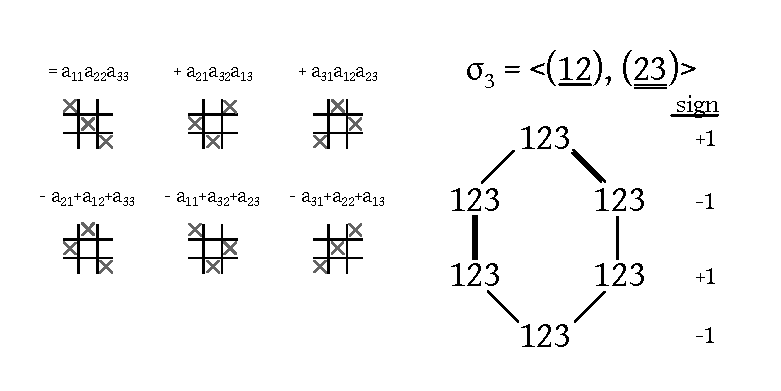
\includegraphics{img/02a_cayley_graph.pdf}
      \caption{Cayley graph (right) and permutation factors in Sarrus' Rule (left) in the 3D case}
      \label{img:cayley}
    \end{center}
  \end{figure}

  By the Cayley-Graph of group $\sigma_3$ we can see that $\sigma_3 = \angel{(\underline{12}), (\underline{\underline{23}})} = -1$.
  \[
    \begin{array}{ccc|cc}
      a_{11} & a_{12} & a_{13} & a_{11} & a_{12} \\
      a_{21} & a_{22} & a_{23} & a_{21} & a_{22} \\
      a_{31} & a_{32} & a_{33} & a_{31} & a_{32}
    \end{array}
  \]

  \emph{Rule of Sarrus} holds only for $n=2$ or $n=3$.
\end{example}

\dateref{2018/03/14}

\begin{Example}[Rule by Sarrus]
  Let $n=2$:
  \[
    \begin{vmatrix} a & b \\ c & d \end{vmatrix} = ad - bc
  \]
  Let $n = 3$:
  \[
    \begin{vmatrix}
      1 & 2 & 5 & 1 & 2 \\
      2 & 5 & 14 & 2 & 5 \\
      5 & 14 & 42 & 5 & 14
    \end{vmatrix}
    = 1
  \]
  \begin{align*}
    &1 \cdot 5 \cdot 42 + 2 \cdot 14 \cdot 5 + 5 \cdot 2 \cdot 14 - 5 \cdot 5 \cdot 5 - 1 \cdot 14 \cdot 14 - 2 \cdot 2 \cdot 42 \\
      &= 14 \cdot (1 \cdot 5 \cdot 3 + 2 \cdot 5 + 5 \cdot 2) - 125 - 14 \cdot (14 + 2 \cdot 2 \cdot 3) \\
      &= 14 \cdot 35 - 125 - 14 \cdot 26 \\
      &= 14 \cdot 9 - 125 = 1
  \end{align*}
  An error in the computation will be enhanced.

  Let $n = 4$.
  $\card{\sigma_n} = 24$ makes consideration of all permutations impractical.
\end{Example}

\begin{lemma} % Lemma 7.32
  Let $A$ be an upper triangular matrix, hence $a_{ij} = 0$ if $i > j$.
  \[ \implies \det(A) = a_{11} a_{22} \dots a_{nn} \]
\end{lemma}
\begin{proof}
  \[ \det(A) = \sum_{\pi \in \sigma_n} (-1)^\pi a_{\pi(1) 1} \dots a_{\pi(n) n} \]
  such that $\pi(j) \leq j \forall j$.
  \[ \implies \operatorname{id} \]
  \begin{align*}
    \pi(j) \leq j \forall j \implies
      &\pi(1) \leq 1 \implies \pi(1) = 1 \\
      &\pi(2) \leq 2 \implies \pi(2) = 2 \\
      &\pi(3) \leq 3 \implies \pi(3) = 3 \\
      &\dots \\
      &\pi(n) \leq n \implies \pi(n) = n \\
  \end{align*}
\end{proof}

\begin{theorem} % 7.33
  Let $A = (a_{ij})$ be a $n\times n$ matrix.
  \begin{enumerate}
    \item Let $z_1, \dots, z_n$ be row vectors of $A$. Then
      \[ \det\begin{bmatrix} z_1 & \ldots \\ \vdots & \\ z_n & \ldots \end{bmatrix} = \det\begin{bmatrix} z_1 & \ldots \\ z_i + \lambda z_j & \ldots \\ \vdots & \\ z_n & \ldots \end{bmatrix} \forall i \neq j, \lambda \in \mathbb K \]
    \item
      Let $S_1, \dots, S_n$ be columns of $A$. Then,
      \[ \det\begin{pmatrix} S_1 & \ldots & S_n \\ \vdots & & \vdots \end{pmatrix} = \det\begin{pmatrix} S_1 & \ldots & S_i + \lambda S_j & \ldots & S_j & \ldots & S_n \\ \vdots & & \vdots & & \vdots & & \vdots \end{pmatrix} \]
  \end{enumerate}
\end{theorem}
\begin{proof}
  \begin{enumerate}
    \item[2.] Proof for column $i$:
      \[ \triangle(s_1, \dots, s_n)= \triangle(s_1, \dots, s_i + \lambda s_j, \dots, s_n) \]
      \[ \left( = \triangle(s_1, \dots, s_i, \dots, s_n) + \lambda \underbrace{\triangle(s_1, \dots, s_j, \dots, s_j, \dots, s_n)}_{=0} \right) \]
    \item[1.] Second proof
      Row form is multiplication from left with matrix of structure
      \[ I + \lambda E_{ij} \qquad i \neq j \]
      \[ \det((I + \lambda E_{ij}) A) = \underbrace{\det(I + \lambda E_{ij})}_{\text{triangular matrix} = 1} \cdot \det(A) \]
  \end{enumerate}
\end{proof}
\begin{example} % Beispiel 7.34
  \[
    \begin{vmatrix}
      % arrow row 1 to row 3, -5
      % arrow row 1 to row 2, -2
      1 & 2 & 5 \\
      2 & 5 & 14 \\
      5 & 14 & 42
    \end{vmatrix}
    =
    \begin{vmatrix}
      % arrow row 2 to row 3, -4
      1 & 2 & 5 \\
      0 & 1 & 4 \\
      0 & 4 & 17
    \end{vmatrix}
    =
    \begin{vmatrix}
      1 & 2 & 5 \\
      0 & 1 & 4 \\
      0 & 0 & 1
    \end{vmatrix}
    = 1
  \]
\end{example}

\begin{Example}
  \[
    \begin{vmatrix}
      % arrow row 1 to row 4, 1
      % arrow row 1 to row 3, -3
      % arrow row 1 to row 2, -2
      1 & 0 & 3 & -2 \\
      2 & 6 & 4 & 1 \\
      3 & 3 & -1 & -1 \\
      -1 & 2 & 4 & 1
    \end{vmatrix}
    =
    \begin{vmatrix}
      % row 3, x2
      % row 4, x3
      1 & 0 & 3 & -2 \\
      0 & 6 & -2 & 5 \\
      0 & 3 & -10 & 5 \\
      0 & 2 & 7 & -1
    \end{vmatrix}
  \] \[
    =
    \frac13 \frac12
    \begin{vmatrix}
      % arrow row 2 to row 3, -1
      % arrow row 2 to row 4, -1
      1 & 0 & 3 & -2 \\
      0 & 6 & -2 & 5 \\
      0 & 6 & -20 & 10 \\
      0 & 6 & 21 & -3
    \end{vmatrix}
    =
    \frac16 % due to column 2
    \begin{vmatrix}
      1 & 0 & 3 & -2 \\
      0 & 6 & -2 & 5 \\
      0 & 0 & -18 & 5 \\
      0 & 0 & 23 & -8
    \end{vmatrix}
    = \frac16 \cdot 6
    \begin{vmatrix}
      % column 4 plus column 3
      1 & 0 & 3 & -2 \\
      0 & 1 & -2 & 5 \\
      0 & 0 & -18 & 5 \\
      0 & 0 & 23 & -8
    \end{vmatrix}
  \] \[
    =
    \begin{vmatrix}
      1 & 0 & -1 & -2 \\
      0 & 1 & 8 & 5 \\
      0 & 0 & -8 & 5 \\
      0 & 0 & 7 & -8
      % arrow row 3 to row 4, +1
    \end{vmatrix}
    =
    \begin{vmatrix}
      % arrow row 4 to row 3, -8
      1 & 0 & -1 & -2 \\
      0 & 1 & 8 & 5 \\
      0 & 0 & -8 & 5 \\
      0 & 0 & -1 & -3
    \end{vmatrix}
    =
    \begin{vmatrix}
      % exchange row 3 and row 4
      1 & 0 & -1 & -2 \\
      0 & 1 & 8 & 5 \\
      0 & 0 & 0 & 29 \\
      0 & 0 & -1 & -3
    \end{vmatrix}
  \] \[
    - \begin{vmatrix}
      1 & 0 & -1 & -2 \\
      0 & 1 & 8 & 5 \\
      0 & 0 &-1 & -3 \\
      0 & 0 & 0 & 29
    \end{vmatrix}
     = 29
  \]
\end{Example}

\begin{Remark}[Laws, discussed so far]
  \[
    \begin{vmatrix}
      z_1 & \ldots \\
      \lambda \cdot z_1 & \ldots \\
      z_n & \ldots
    \end{vmatrix}
    = \lambda \begin{vmatrix}
      z_1 & \ldots \\
      \vdots & \\
      z_k & \ldots \\
      \vdots & \\
      z_n & \ldots
    \end{vmatrix}
  \] \[
    \begin{vmatrix}
      z_1 & \ldots \\
      z_1 + \lambda z_j & \ldots \\
      z_n & \ldots
    \end{vmatrix}
    = \begin{vmatrix}
      z_1 & \ldots \\
      \vdots & \\
      z_i & \ldots \\
      \vdots & \\
      z_n & \ldots
    \end{vmatrix}
    \qquad (i \neq j)
  \] \[
    \begin{vmatrix}
      z_1 & \ldots \\
      \vdots & \\
      z_i & \ldots \\
      \vdots & \\
      z_j & \ldots \\
      \vdots & \\
      z_n & \ldots
    \end{vmatrix}
    = -\begin{vmatrix}
      z_1 & \ldots \\
      \vdots & \\
      z_j & \ldots \\
      \vdots & \\
      z_i & \ldots \\
      \vdots & \\
      z_n & \ldots
    \end{vmatrix}
  \] \[
    \begin{vmatrix}
      a_{11} & \ldots &        &        & \\
             & a_{22} & \ldots &        & \\
             &        & a_{33} & \ldots & \\
             &        &        & \ddots & \\
           0 &        &        &        & a_{nn}
    \end{vmatrix}
    = a_{11} \cdot a_{nn}
  \]
\end{Remark}
\begin{lemma}
  \begin{enumerate}
    \item \[
      \begin{vmatrix}
        a_{11} & * & * & * & \\
        0 &    &   &   &   & \\
        0 &    &   & B &   & \\
        0 &    &   &   &   &
      \end{vmatrix}
      = a_{11} \cdot \det(B)
    \]
    \item \[
      \begin{vmatrix}
        &   &   &   & 0 \\
        &   & B &   & 0 \\
        &   &   &   & 0 \\
        & * & * & * & a_{nn}
      \end{vmatrix}
      = \det(B) \cdot a_{nn}
    \]
    \item If there are individual square matrices ($A_1, A_2, \dots, A_k$) along the diagonal of a matrix,
  the determinant of the matrix is the product of the determinant of the submatrices.
  \[ \det(A) = \det(A_1) \cdot \det(A_2) \cdot \ldots \cdot \det(A_k) \]
  \end{enumerate}
\end{lemma}

\begin{proof}
  We only prove the second property.

  All permutations which do not map index 1 to 1, introduce a factor zero making the product zero.
  If index 1 is mapped to 1, the product in Leibniz' formula is multiplied with $a_{11}$ in all permutations.
  We can extract factor $a_{11}$ and get the determinant of $B$ multiplied with $a_{11}$.
  \begin{align*}
    \begin{vmatrix}
             &         &           & 0  \\
      B      &         &           & \vdots \\
             &         &           & 0  \\
      a_{n,1} & \ldots & a_{n,n-1} & a_{n,n}
    \end{vmatrix}
    &= \sum_{\pi \in \sigma_n} (-1)^{\pi} a_{\pi(1) 1} \dots a_{\pi(n) n} \\
    &= \sum_{\pi' \in \sigma_{n-1}} (-1)^{\pi'} a_{\pi'(1) 1} \dots a_{\pi'(n-1) n-1} \cdot a_{nn} \\
    &= \det(B) \cdot a_{nn}
  \end{align*}
  \[ \setdef{\pi \in \sigma_n}{\pi(n) = n} \]
  \[ \pi(n) = n \]
  \[
    B = \begin{pmatrix}
      a_{11} & \ldots & a_{1,n-1} \\
      \vdots &        & \\
      a_{n-1,1} & \ldots & a_{n,n-1}
    \end{pmatrix}
  \]

  Same idea: If
  \[
    A = \begin{bmatrix}
      & 0 & \\
      & \vdots & \\
      & 0 & \\
      \vdots & a_{ij} & \vdots \\
      & 0 & \\
      & \vdots & \\
      & 0 &
    \end{bmatrix}
  \]
  Exchange the $i$-th row with the last row.
  \[
    = \pm 1 \begin{bmatrix}
      & 0 \\
      & \vdots \\
      & 0 \\
      \cdots & 0 \\
      & 0 \\
      & \vdots \\
      & a_{ij} \\
    \end{bmatrix}
  \]
\end{proof}

\begin{definition}
  % Definition 7.36
  \[ A \in \mathbb K^{n\times n} \]
  $A_{k,l}$ is an $(n-1) \times (n-1)$ matrix, that is created by omitting the $k$-th row and $l$-th column.
  \[
    \begin{bmatrix}
      a_{1,1} & \ldots & a_{1,l-1} & a_{1,l+1} & \ldots & a_{1,n} \\
      \vdots  &        &           &           &        & \vdots \\
      a_{k-1,1} & \ldots & a_{k-1,l-1} & a_{k-1,l+1} & \ldots & a_{k-1,n} \\
      a_{k+1,1} & \ldots & a_{k+1,l-1} & a_{k+1,l+1} & \ldots & a_{k+1,n} \\
      \vdots  &        &           &           &        & \vdots \\
      a_{n,1} & \ldots & a_{n,l-1} & a_{n,l+1} & \ldots & a_{n,n} \\
    \end{bmatrix}
  \]
\end{definition}

\begin{Person}
  Pierre-Simon Laplace (1749--1827)
\end{Person}
\begin{definition}[Laplace expansion] % Definition 7.37
  In German, this theorem is called \foreignlanguage{german}{Entwicklungssatz von Laplace}.
  
  Let $l$ be fixed.
  \[ \det(A) = \sum_{k=1}^n a_{kl} (-1)^{k+l} \det(A_{kl}) \qquad \text{\enquote{Expansion along column $l$}} \]

  Let $k$ be fixed.
  \[ \det(A) = \sum_{l=1}^n a_{kl} (-1)^{k+l} \det(A_{kl}) \qquad \text{\enquote{Expansion along row $k$}} \]
\end{definition}

\begin{example} % Beispiel 7.38
  \[
    \begin{vmatrix}
      1 & 2 & 5 \\
      2 & 5 & 14 \\
      5 & 14 & 42
    \end{vmatrix}
    = \sum_{l=1}^3 (-1)^{1+l} \det(A_{1l})
    \qquad \text{ for $k=1$ fixed}
  \]
  \[ = 1 \begin{vmatrix} 5 & 14 \\ 14 & 42 \end{vmatrix} - 2 \cdot \begin{vmatrix} 2 & 14 \\ 5 & 42 \end{vmatrix} + 5 \cdot \begin{vmatrix} 2 & 5 \\ 5 & 14 \end{vmatrix} \]
  \[ = 1 \cdot (5 \cdot 42 - 14 \cdot 14) - 2 (2 \cdot 42 - 5 \cdot 14) + 5 \cdot (2 \cdot 14 - 5 \cdot 9) \]
  \[ = 1 \cdot (5 \cdot 3 \cdot 14 - 14 \cdot 14) - 2 \cdot (2 \cdot 3 \cdot 13 - 5 \cdot 14) \]
  \[ = 14 - 2 \cdot 14 + 5 \cdot 15 = 1 \]

  Consider $k=2$.
  \[
    -2 \cdot \begin{vmatrix} 2 & 5 \\ 14 & 42 \end{vmatrix} + 5 \cdot \begin{vmatrix} 1 & 5 \\ 5 & 42 \end{vmatrix} - 14 \cdot \begin{vmatrix} 1 & 2 \\ 5 & 14 \end{vmatrix}
  \] \[
    = -2 (3 \cdot 14 \cdot 2 - 14 \cdot 5) + 5 \cdot (42 - 25) - 14 \cdot (14 - 10)
  \] \[
    = -2 \cdot 14 + 5 \cdot 17 - 4 \cdot 14 = -28 +85 -56 = 85 - 84 = 1
  \]
\end{example}

\dateref{2018/03/19}

Review:
\begin{itemize}
  \item Determinants are multilinear (in rows and columns)
  \item Determinants switches its sign if two rows or row columns are exchanged
  \item $\triangle(s_1, \dots, s_n) = (-1)^\pi \triangle(s_{\pi(1)}, \dots, s_{\pi(n)})$ where $s_i$ are column vectors
  \item
    \[
      \begin{vmatrix}
        a_{11} & 0 & \dots & 0 \\
        * &        &       & \\
        \vdots &   &  B    & \\
        * &        &       &
      \end{vmatrix}
      = a_{11} \cdot \det{B}
      \qquad B = A_{11}
    \]
    where $A_{kl}$ is the $(n-1) \times (n-1)$ matrix created by removal of the $k$-th row and $l$-th column.
    This is a special case of Laplace expansion.
\end{itemize}

\subsection{Laplace expansion}
\begin{align*}
  \det{A} &= \sum_{k=1}^n (-1)^{k+l} a_{kl} \cdot \det{A_{kl}} & \text{ for fixed } l \in \set{1, \dots, n} \\
          &= \sum_{l=1}^n (-1)^{k+l} a_{kl} \cdot \det{A_{kl}} & \text{ for fixed } k \in \set{1, \dots, n}
\end{align*}

So in the case of (a very classic example)
\[
  \begin{vmatrix}
    a_{11} & 0 & \dots & 0 \\
    * &        &       & \\
    \vdots &   &  B    & \\
    * &        &       &
  \end{vmatrix}
  = a_{11} \cdot (-1)^{1 + 1} \cdot \det{A_{11}}
\]
for fixed $k=1$:
\[ \sum_{l=1}^n (-1)^{1 + l} \underbrace{a_{1l}}_{=0 \text{ for } l > 1} \det{A_{1l}} \]

\begin{proof}
  Let $l \in \set{1, \dots, n}$ be fixed.
  Let $e_k$ be a unit vector.
  For the $l$-th column,
  \[ s_l = \sum_{k=1}^n a_{kl} e_k = \begin{pmatrix} a_{1l} \\ a_{2l} \\ \vdots \\ a_{nl} \end{pmatrix} \]
  \begin{align*}
    \det(A) &= \triangle(s_1, s_2, \dots, s_{l-1}, \sum_{k=1}^n a_{kl} \cdot e_k, s_{l+1}, \dots, s_n) \\
            &= \sum_{k=1}^n a_{kl} \triangle(s_1, \dots, s_{l-1}, e_k, s_{l+1}, \dots, s_n) \\
            &= \sum_{k=1}^n a_{kl} \begin{vmatrix}
              a_{11} & a_{12} & \vdots & a_{1,l-1} & 0 & a_{1,l+1} & \dots & a_{1n} \\
              a_{21} & a_{22} & \vdots & a_{2,l-1} & \vdots & \vdots &  & \vdots \\
              \vdots & \vdots & \vdots & \vdots & \vdots & \vdots &  & \vdots \\
              \vdots & \vdots & \vdots & \vdots & 0 & \vdots &  & \vdots \\
              \vdots & \vdots & \vdots & \vdots & 1 & \vdots &  & \vdots \\
              \vdots & \vdots & \vdots & \vdots & 0 & \vdots &  & \vdots \\
              \vdots & \vdots & \vdots & \vdots & \vdots & \vdots &  & \vdots \\
              a_{n1} & a_{n2} & \vdots & a_{n,l-1} & 0 & a_{n,l+1} & \dots & a_{nn} \\
            \end{vmatrix} \\
    \intertext{
      Recognize the one in row $k$. We consecutively exchange row $k$ with the row above until it becomes row 1.
      This gives $k-1$ exchanges. Hence a cycle $(1 \dots k)$. This gives $\sign = (-1)^{k-1}$.
    }
    &= \sum_{k=1}^n a_{kl} (-1)^{k-1} \begin{vmatrix}
      a_{k1} & a_{k2} & \dots & a_{k,l-1} & 1 & a_{k,l+1} & \dots & a_{kn} \\
      a_{11} & a_{12} & \dots &           & 0 &           &       & a_{1n} \\
      \vdots & \vdots & \dots &           & 0 &           &       & \vdots \\
      a_{k-1,1} & a_{k-1,2} & \dots &           & 0 &           &       & a_{k-1,n} \\
      a_{k+1,1} & a_{k+1,2} & \dots &           & 0 &           &       & a_{k+1,n} \\
      \vdots & \vdots & \dots &           & 0 &           &       & \vdots \\
      a_{n1} & a_{n2} & \dots &           & 0 &           &       & a_{nn}
    \end{vmatrix} \\
    \intertext{
      Now we can do $l-1$ column exchanges to move the one into the first column.
      This gives a cycle $(1, 2, \dots, l)$ and $\sign = (-1)^{l-1}$
    }
    &= \sum_{k=1}^n a_{kl} (-1)^{k-1} (-1)^{l-1}   \begin{vmatrix}
      1 & a_{k1} & a_{k2} & \dots & a_{k,l-1} & a_{k,l+1} & \dots & a_{k,n} \\
      0 & a_{11} & a_{12} & \dots & a_{1,l-1} & a_{1,l+1} & \dots & a_{1,n} \\
      0 & \vdots & \vdots & \vdots& \vdots    & \vdots    & \vdots& a_{2,n} \\
      0 & a_{k-1,1} & a_{k-1,2} & \dots & a_{k-1,l-1} & a_{k-1,l+1} & \dots & a_{k-1,n} \\
      0 & a_{k+1,1} & a_{k+1,2} & \dots & a_{k+1,l-1} & a_{k+1,l+1} & \dots & a_{k+1,n} \\
      0 & \vdots & \vdots & \vdots& \vdots    & \vdots    & \vdots& a_{2,n} \\
      0 & a_{n1} & a_{n2} & \dots & a_{nl-1} & a_{nl+1} & \dots & a_{nn} \\
    \end{vmatrix} \\
    \intertext{
      where the $k$-th row and $l$-th column is removed
    }
    &= \sum_{k=1}^n (-1)^{k+l} a_{kl} \det{A_{kl}}
  \end{align*}
\end{proof}

\begin{example} % Beispiel 7.38
  Let $A = (a_{kl})_{\substack{1 \leq k \leq n \\ 1 \leq l \leq n}} = (-1)^{k+l}$.
  \[
    A = \begin{pmatrix}
      +1 & -1 & +1 \\
      -1 & +1 & -1 \\
      +1 & -1 & +1
    \end{pmatrix}
  \]
\end{example}

\index{Cofactor}
\index{Complementary matrix}
\index{Adjugate matrix}
\begin{theorem} % Satz 7.39
  $\hat{a}_{kl} \coloneqq (-1)^{k+l} \det{A_{lk}}$ is called \emph{cofactor}.
  \[ \hat{A} = \begin{bmatrix} \hat{a}_{kl} \end{bmatrix}_{k,l=1}^n \]
  is called \emph{complementary matrix} or \emph{adjugate matrix} of $A$.
  \begin{align*}
    \hat{a}_{kl}
    &= (-1)^{k+l} \det \text{ (the matrix without row $l$ and column $k$) } \\
    &= (-1)^{k+l} \det{A_{lk}} = \frac{\partial}{\partial a_{lk}} \det{A}
  \end{align*}
  Then it holds that
  \[ A^{-1} = \frac{1}{\det{A}} \hat{A} \]
\end{theorem}

\begin{proof}
  Show that $\hat{A} \cdot A = I \cdot \det(A)$.
  Let $B = \hat{A} \cdot A$.
  \[ b_{kl} = \sum_{i=1}^n \hat{a}_{ki} \cdot a_{il} = \sum_{i=1}^n (-1)^{k+i} \det{A_{ik}} \cdot a_{il} \]
  \begin{description}
    \item[Case $\mathbf{k=l}$]
      \[
        b_{ll} = \sum_{i=1}^n (-1)^{l+i} \det{A_{il}} \cdot a_{il}
          \underbrace{=}_{\substack{\text{Laplace expansion} \\ \text{with $l$-th column}}} \det{A}
      \]
    \item[Case $\mathbf{k \neq l}$] Without loss of generality: $k < l$.
      \begin{align*}
        b_{kl} &= \sum_{i=1}^n \det(A_{ik}) (-1)^{k+i} a_{il} \\
        \intertext{unlike Laplace expansion along $k$-th column, this expression uses column $l$. So column $k$ is omitted and column $l$ is used twice.}
               &= \det\begin{bmatrix}
                 a_{11} & \dots & a_{1l} & \dots & a_{1l} & \dots & a_{1n} \\
                 \vdots &       & \vdots &       & \vdots &       & \vdots \\
                 a_{n1} & \dots & a_{nl} & \dots & a_{nl} & \dots & a_{nn}
               \end{bmatrix} \\
        \intertext{where the left $l$-column is column $k$ replaced with values of column $l$ and the right $l$-column is the original column $l$}
               &\underbrace{=}_{\substack{\text{two equal} \\ \text{columns}}} 0
        %\intertext{
        %  (i.e. matrix $A$ with $k$-th column replaced by $l$-th column)
        %  expanded by $k$-th row.
        %}
        %\det{A} &= \sum_{i=1}^n (-1)^{k+i} \det(A_{ik}) \cdot a_{ik} \\
        %\tilde{A} &= \text{ (matrix $A$ replacing $k$-th column with $l$-th column)} \\
        %\det{\tilde{A}} &= \sum_{i=1}^n (-1)^{k+i} \det(A_{ik}) \cdot a_{il}
      \end{align*}
      Thus, the sum of both cases is $b_{kl} = \det(A) + 0$. Thus $B = \hat A \cdot A = I \cdot \det(A)$.
  \end{description}
\end{proof}

\begin{example}[Small inverse matrices] % Anwendung 7.40
  Let $n=2$.
  \begin{align*}
    \begin{bmatrix}
     a & b \\
     c & d
    \end{bmatrix}
    = \frac{1}{ad - bc} \cdot
    \begin{bmatrix} d & -b \\ -c & a \end{bmatrix}
  \end{align*}
  \[ \hat{a}_{11} = (-1)^{1+1} \cdot \det{A_{11}} \qquad \hat{a}_{21} = (-1)^{2+1} \cdot \det{A_{12}} \]
  \[ \hat{a}_{12} = (-1)^{1+2} \cdot \det{A_{21}} \qquad \hat{a}_{22} = (-1)^{2+2} \cdot \det{A_{22}} \]
\end{example}

\begin{Remark}[Cayley 1855]
  \[
    A^{-1} = \frac{1}{\nabla} \begin{bmatrix} \partial_a \nabla & \partial_c \nabla \\ \partial_b \nabla & \partial_d \nabla \end{bmatrix} \qquad
    \nabla f = \begin{bmatrix} \frac{\partial f}{\partial x_1} \\ \vdots \\ \frac{\partial f}{\partial x_n} \end{bmatrix}
  \]
\end{Remark}

\begin{Example}
  Let $n=3$.
  \[
    \begin{bmatrix}
      a_{11} & a_{12} & a_{13} \\
      a_{21} & a_{22} & a_{23} \\
      a_{31} & a_{32} & a_{33}
    \end{bmatrix}^{-1}
    = \frac{1}{\det(A)}
    \begin{bmatrix}
      \begin{vmatrix} a_{22} & a_{23} \\ a_{32} & a_{33} \end{vmatrix} & -\begin{vmatrix} a_{12} & a_{13} \\ a_{32} & a_{33} \end{vmatrix} & \begin{vmatrix} a_{12} & a_{13} \\ a_{22} & a_{23} \end{vmatrix} \\
      -\begin{vmatrix} a_{21} & a_{23} \\ a_{31} & a_{33} \end{vmatrix} & \begin{vmatrix} a_{11} & a_{13} \\ a_{31} & a_{33} \end{vmatrix} & -\begin{vmatrix} a_{11} & a_{13} \\ a_{21} & a_{23} \end{vmatrix} \\
      \begin{vmatrix} a_{21} & a_{22} \\ a_{31} & a_{32} \end{vmatrix} & -\begin{vmatrix} a_{11} & a_{12} \\ a_{31} & a_{32} \end{vmatrix} & \begin{vmatrix} a_{11} & a_{12} \\ a_{21} & a_{22} \end{vmatrix}
    \end{bmatrix}
  \]
\end{Example}

\begin{corollary}
  Let $A \in \mathbb Z^{n\times n}$.
  If $\det{A} = 1 \implies A^{-1} \in \mathbb Z^{n \times n}$.

  Let $A \in \mathbb Z^{n \times n}$ and $\det{A} = 1$.
  Let $B \in \mathbb Z^{n \times n}$ and $\det{B} = 1$.
  \[ \implies \det(A \cdot B) = 1 \qquad \implies \det(A^{-1}) = 1 \]
\end{corollary}

\index{Special linear group}
\begin{definition}
  Integer matrices with $\det = 1$ define a group called \emph{special linear group}.
  \[ \operatorname{SL}(n, \mathbb Z) = \setdef{A \in \mathbb Z^{n \times n}}{\det{A} = 1} \]
  Or in general for a ring $R$:
  \[ \operatorname{SL}(n, R) = \setdef{A \in R^{n \times n}}{\det{A} = 1} \]
\end{definition}

\subsection{Cramer's Rule}

\begin{Person}
  Gabriel Cramer (1704--1752)
\end{Person}

\begin{theorem}[Cramer's Rule]
  Show by Cramer in 1750, by McLaurin 1748 for $n \leq 3$.

  Let $A$ be a invertible matrix with column vectors $a_1, \dots, a_n$.
  Then the solution $Ax = b$ ($\implies x = A^{-1} b$ has a unique solution) is given by
  \begin{align*}
    x_i &= \frac{\triangle (a_1, \dots, a_{i-1}, b, a_{i+1}, \dots, a_n)}{\triangle (a_1, \dots, a_n)} \\
        &= \frac{\det\left(\begin{bmatrix} a_1 & \dots & a_{i-1} & b & a_{i+1} & \dots & a_{n} \\ \vdots &  & \vdots & \vdots & \vdots & & \vdots \end{bmatrix}\right)}{\det{A}}
  \end{align*}
  $n+1$ determinants of form $n \times n$. In practice infeasible except for small matrices.
\end{theorem}

\begin{proof}[Geometrical proof for $n=2$]
  \[ A = \begin{pmatrix} a_1 & a_2 \\ \vdots & \vdots \end{pmatrix} \]
  \[ Ax = b \qquad a_1 \cdot x + a_2 \cdot x_2 = b \]
  \[ \triangle (a_1, a_2) = A(a_1, a_2) \]
  where $A$ is the area function. Compare with Figure~\ref{img:geomn2}.

  \begin{figure}[h]
    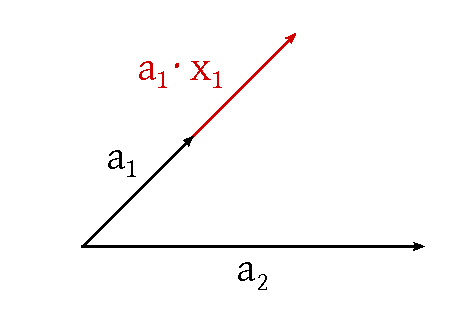
\includegraphics{img/02b_geometrical_proof_for_n2.pdf}
    \caption{Geometrical proof for $n=2$. $\triangle(a_1, a_2)$ is the area of the parallelogram}
    \label{img:geomn2}
  \end{figure}

  \[ \triangle(b, a_2) = A(b, a_2) = \triangle(x_1 \cdot a_1, a_2) = x_1 \cdot \triangle(a_1, a_2) \]
  \[ \implies x_1 = \frac{\triangle (b, a_2)}{\triangle (a_1, a_2)} \]
\end{proof}

\begin{proof}[Generic proof]
  Let $x = A^{-1} \cdot b = \frac{1}{\det{A}} \cdot \hat{A} \cdot b$.
  \begin{align*}
    x_i &= \frac{1}{\det{A}} \cdot \sum_{k=1}^n \hat{a}_{ik} b_k \\
        &= \frac{1}{\det{A}} \sum_{k=1}^n (-1)^{i+k} \det{A_{ki}} \cdot b_k \\
        &\underbrace{=}_{\substack{\text{see proof of} \\ \text{Laplace expansion}}} \frac{1}{\det{A}} \sum_{k=1}^n \triangle(a_1, \dots, a_{i-1}, e_k, a_{i+1}, \dots, a_n) b_k \\
        &= \frac{\triangle(a_1, \dots, a_{i-1}, b, a_{i+1}, \dots, a_n)}{\det{A}}
  \end{align*}
\end{proof}

\begin{Example}
  \begin{align*}
    2x_1 + x_2 &= 7 \\
    x_1 - 3x_2 &= 0 \\
  \end{align*}%
%
  \[ A = \begin{bmatrix} 2 & 1 \\ 1 & -3 \end{bmatrix} \]
  \[ \det(A) = 2 \cdot (-3) - 1 = -7 \]

  \[ x_1 = -\frac17 \begin{vmatrix} 7 & 1 \\ 0 & -3 \end{vmatrix} = 3 \]
  \[ x_2 = -\frac17 \begin{vmatrix} 2 & 7 \\ 1 & 0 \end{vmatrix} = 1 \]
\end{Example}

\begin{Remark}
  For large $n$ (hence $n \geq 4$), Cramer's Rule is impractical (tiresome and unstable).
  But it helps with theoretical considerations.
  \begin{enumerate}
    \item The map $A \mapsto \det{A}$ is continuous and differentiable.
    \item if $\det{A} \neq 0 \implies$ the set of invertible matrices is open\footnote{Hence for all invertible $A$, there exists some neighborhood such that all matrices in this neighborhood are invertible. \[ \text{e.g. } d(A, B) = \max_{i,j} \card{a_{ij} - b_{ij}} \]}
    \item The solution of system $Ax = b$ depends continuously on $a_{ij}$ and $b_i$~\footnote{
      This justifies why Computational Mathematics (dt. \foreignlanguage{german}{Numerik}) is practical and interesting
      \[ \forall \varepsilon \exists \delta: d(b, b') < \delta \implies d(x, x') < \varepsilon \]
    }
  \end{enumerate}
\end{Remark}

\section{Inner products}

\subsection{Definition}

\begin{definition} % 8.1
  \[ \mathbb R^3: \norm{\begin{pmatrix} a_1 \\ a_2 \\ a_3 \end{pmatrix}} = \sqrt{a_1^2 + a_2^2 + a_3^2} \]
  By Pythagorem Theorem
\end{definition}

\begin{proof}[Geometrical proof of the Pythagorem Theorem]
  Claim: $a^2 + b^2 = c^2$

  \begin{figure}[!ht]
    \begin{center}
      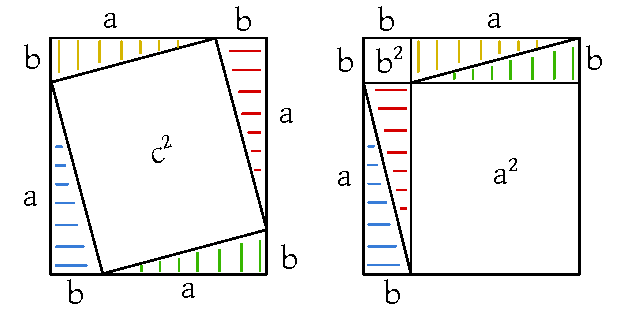
\includegraphics{img/03_pytha.pdf}
      \caption{Proof construction of the Pythagorem Theorem}
      \label{fig:pytha}
    \end{center}
  \end{figure}
\end{proof}

\dateref{2018/03/21}

The norm is given by
\[ \norm{\begin{pmatrix} a_1 \\ a_2 \\ a_3 \end{pmatrix}} = \sqrt{a_1^2 + a_2^2 + a_3^2} \]

\begin{Definition}[Scalar product in $\mathbb R^2/\mathbb R^3$]
  \[ \angel{a, b} \coloneqq \norm{a} \cdot \norm{b} \cdot \cos{\theta} \]
  where $\theta$ is the angle between vector $a$ and $b$.
\end{Definition}

\begin{Theorem}
  $\angel{a,a} = \norm{a}^2$
\end{Theorem}

\begin{Remark}
  Recall that
  \[ \cos{0} = 1 \qquad \cos{\frac\pi2} = 0 \qquad \cos{\pi} = -1 \qquad \cos{\frac32 \pi} = 0 \]
  \[ \sin{0} = 0 \qquad \sin{\frac\pi2} = 1 \qquad \sin{\pi} = 0 \qquad \sin{\frac32 \pi} = -1 \]

  \[ \sin\theta = \cos(\theta - \frac\pi2) \]
  \[ \cos(\pi - \theta) = -\cos(\theta) \]
  \[ \sin(-\theta) = \cos(\theta) \]
  \[ \sin(\pi - \theta) = \sin(\theta) \]
  \[ \sin(-\theta) = -\sin(\theta) \]
\end{Remark}

\begin{theorem} % Satz 8.2
  \begin{enumerate}
    \item $\angel{a,a} = \norm{a}^2$
    \item $\angel{a,a} = 0 \iff a = 0$
    \item $\angel{a,b} = 0 \iff a = 0 \lor b = 0 \lor \theta = \frac\pi2 \lor \theta = \frac32 \pi$, hence orthogonal
    \item $\angel{a,b} > 0 \iff$ acute angle
    \item $\angel{a,b} < 0 \iff$ obtuse angle (dt. \foreignlanguage{german}{stumpf})
  \end{enumerate}
\end{theorem}

\begin{theorem} % Satz 8.3
  \label{satz83}
  \begin{enumerate}
    \item $\angel{a,b} = \angel{b,a}$
    \item $\angel{\lambda a, b} = \lambda \cdot \angel{a, b} = \angel{a, \lambda \cdot b}$
    \item $\angel{a+b, c} = \angel{a,c} + \angel{b, c}$
  \end{enumerate}
  Thus, linear in $a$ and $b$. Thus, bilinear.
\end{theorem}

\begin{proof}
  \begin{enumerate}
    \item $\angel{a, b} = \norm a \norm b \cdot \cos\theta = \norm b \norm a \cdot \cos\theta = \angel{b, a}$
    \item
      Assume $\lambda > 0$. Angle stays the same.
      \[ \angel{\lambda a, b} = \norm{\lambda a} \cdot \norm{b} \cdot \cos\theta = \lambda \cdot \norm{a} \cdot \norm{b} \cdot \cos\theta \]
      Assume $\lambda < 0$. $\theta$ becomes $\pi - \theta$.
      \[ \angel{\lambda a, b} = \norm{\lambda a} \cdot \norm{b} \cdot \cos(\pi - \theta) = \card{\lambda} \cdot \norm{a} \cdot \norm{b} \cdot (-\cos(\theta)) = \lambda \cdot \norm a \cdot \norm b \]
    \item
      Let $\norm{c} = 1$. $\angel{a,c} = \norm a \cdot \cos\theta$.
      \[ \angel{a+b, c} = \angel{a,c} + \angel{b,c} \]
      Projections will add up.

      In the generic case:
      \[ \angel{a+b, c} = \angel{a+b, \norm c \cdot \frac{c}{\norm{c}}} \underbrace{=}_{\text{by (2.)}} \norm c \angel{a+b, \frac{c}{\norm{c}}} \]
%          &= \norm c \cdot \left(\angel{a, \frac{c}{\norm{c}} + \angel{b, \frac{c}{\norm{c}}\right) \\
%          &= \angel{a, c} + \angel{b, c}
  \end{enumerate}
\end{proof}

\begin{theorem} % Satz 8.4
  \[ \angel{\begin{pmatrix} a_1 \\ a_2 \\ a_3 \end{pmatrix}, \begin{pmatrix} b_1 \\ b_2 \\ b_3 \end{pmatrix}} = a_1 b_1 + a_2 b_2 + a_3 b_3 \]
\end{theorem}

\begin{proof}
  \begin{align*}
    \angel{a,b} &= \angel{a_1 e_1 + a_2 e_2 + a_3 e_3, b} \\
      &= a_1 \angel{e_1, b} + a_2 \angel{e_2, b} + a_3 \angel{e_3, b} \\
      &= a_1 b_1 + a_2 b_2 + a_3 b_3 \\
    \angel{e_i,b} &= \angel{e_i, b_1 e_1 + b_2 e_2 + b_3 e_3} \\
      &= b_1 \angel{e_i, e_1} + b_2 \angel{e_i, e_2} + b_3 \angel{e_i, e_3} \\
      &= b_1 \delta_{i1} + b_2 \delta_{i2} + b_3 \cdot \delta_{i3} \qquad \text{ with } \delta \text{ as Kronecker delta} \\
      &= b_i
  \end{align*}
\end{proof}

In this chapter, we will talk about vector spaces in which we will discuss scalar products with properties 1--3 from Theorem~\ref{satz83}.
\begin{align*}
  \text{in } \mathbb R^n: &\angel{x,y} = \sum_{i=1}^n x_i y_i \\
  \text{in } V \subseteq \mathbb R^\infty: &\angel{x,y} = \sum_{i=1}^\infty x_i y_i \qquad \text{ if convergent!}
\end{align*}
For this space, $(e_i)_{i \in \mathbb N}$ is a basis.
\[ \text{in } C[a,b] \qquad \angel{f,g} = \int f(x) g(x) \, dx \]
is the Delta function.

Or better: $(\sin{nx})_{n \in \mathbb N} \cup (\cos{nx})_{n \in \mathbb N}$.

\[ \int_0^{2\pi} \sin(nx) \cos(mx) \, dx = 0 \forall m,n \]
\[ \int_0^{2\pi} \sin(nx) \sin(mx) \, dx = 0 \text{ if } m \neq n \]

\begin{Person}
  Jean-Baptiste Joseph Fourier (1768/03/21--1830/05/16)
\end{Person}

\begin{theorem}[1822 Fourier]
  Every function $f$ in $[0,2\pi]$ can be denoted as
  \begin{align*}
    f(x) &= \sum_{n=0}^\infty a_n \cos(nx) + \sum_{n=1}^\infty b_n \sin(nx) \\
    a_n &= \angel{f, \cos(nx)} = \int_0^{2\pi} f(x) \cos(nx) \, dx \\
    b_n &= \angel{f, \sin(nx)} = \int_0^{2\pi} f(x) \sin(nx) \, dx
  \end{align*}
  This theorem cannot be proven, because it depends on the definition of \enquote{function}.
  The answer to the question, which functions satisfy this theorem, is an open research topic.
\end{theorem}

\subsection{Law of cosines}

\begin{theorem}[Law of cosines]
  In German, \foreignlanguage{german}{\enquote{Kosinussatz}}.

  \[ c^2 = a^2 + b^2 - 2ab \cos{\gamma} \]
  \begin{align*}
    \norm{\rh{c}}^2 &= \norm{\rh{b} - \rh{a}}^2 \\
      &= \angel{\rh{b} - \rh{a}, \rh{b} - \rh{a}} \\
      &= \angel{\rh{b}, \rh{b}} - \angel{\rh{a}, \rh{b}} - \angel{\rh{b}, \rh{a}} + \angel{\rh{a}, \rh{a}} \\
      &= \norm{b}^2 - 2 \norm{a} \norm{b} \cos\gamma + \norm{a}^2
  \end{align*}
\end{theorem}
\[ \norm a \cdot \norm b \cdot \sin\theta = \text{ area of the spanned parallelogram} \]

How to find an orthogonal vector?

\begin{Remark}[Orthogonal vector in $\mathbb R^2$]
  Find $\vec{b}$ such that $\angel{\rh{a}, \rh{b}} = 0$, $a_1 b_1 + a_2 b_2 = 0$. For example, $b_1 = a_2$ and $b_2 = -a_1$.
  \[ \rh{a} = \begin{pmatrix} a_1 \\ a_2 \end{pmatrix} \qquad \rh{b} = \begin{pmatrix} a_2 \\ -a_1 \end{pmatrix} \]
\end{Remark}

\subsection{Outer product}

\index{Outer product}
\index{Cross product}
\begin{definition} % 8.7
  Called \emph{outer product} (only in $\mathbb R^3$) or \emph{cross product}.

  Let $a, b \in \mathbb R^3$ and let $a \times b$ be the vector which
  \begin{enumerate}
    \item $\norm{a \times b} = \norm{a} \cdot \norm{b} \cdot \sin{\theta}$ is the area of the spanned parallelogram.
    \item $a \times b \bot a \text{ and } a \times b \bot b
      \iff \angel{a \times b, a} = 0 \text{ and } \angel{a \times b, b} = 0$
    \item $(a, b, a \times b)$ is clockwise.
      \[ \text{When does } a \times b = 0 \text{ hold? } a = 0, b = 0, \sin\theta = 0, \text{ hence } \theta = 0 \lor \theta = \pi \]
      \[ \iff a,b \text{ are linear independent} \]
  \end{enumerate}
\end{definition}

\begin{theorem}
  \begin{itemize}
    \item $b \times a = -a \times b$
    \item $(\lambda a) \times b = \lambda (a \times b) = a \times (\lambda b)$
    \item $(a + b) \times c = a \times c + b \times c$
  \end{itemize}
\end{theorem}

\begin{proof}
  \begin{itemize}
    \item Orientation swaps. Consider the right-hand rule. If you assign $b$ to your index finger, $a$ to your middle finger, you retrieve direction $b \times a$ with the thumb. Now assign $a$ (index finger) and $b$ (middle finger) and you retrieve the opposite direction, namely $- \left(b \times a\right)$.
    \item If $\lambda > 0$, it follows immediate.
      If $\lambda < 0$, lengths stay the same, but orientation swaps.
    \item If $c = 0$, it is trivial. If $c \neq 0$,
      \begin{figure}[!ht]
        \begin{center}
          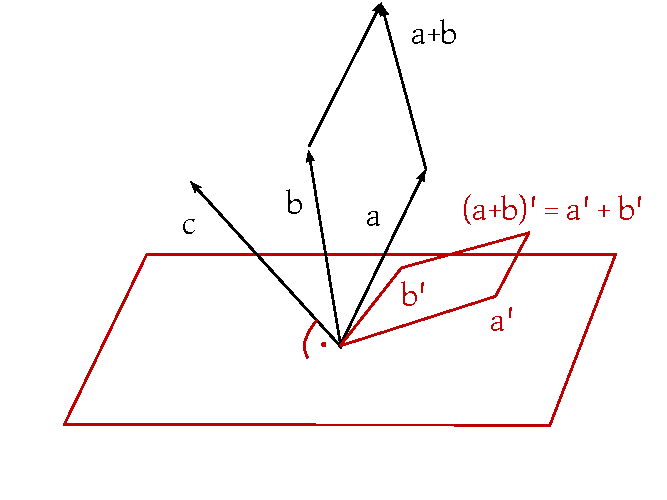
\includegraphics{img/04_apbmc_eq_amcpbmc.pdf}
        \end{center}
      \end{figure}
      E is the plane orthogonal to $c$. $a'$ and $b'$ are projections of $a$ and $b$ to $E$.

      \begin{enumerate}
        \item $(a+b)' = a' + b'$
        \item $a \times c = a' \times c$.
          \begin{align*}
            \norm{a \times c} &= \norm a \norm c \cdot \sin\theta \\
              &= \norm{a'} \cdot \norm{c} \\
              &= \norm{a' \times c}
          \end{align*}
          \begin{itemize}
            \item Orientation of $a \times c$ and $a' \times c$ is the same
            \item The plane, spanned by $c$ and $a$, is also spanned by $c$ and $a'$
          \end{itemize}

          \[ \norm{a'} = \norm{a} \cdot \underbrace{\cos\left(\frac\pi2\right)}_{=\sin\theta} - \theta) \]
          Hence,
          \[ (a + b) \times c = (a + b)' \times c = (a' + b') \times c \stackrel!= a' \times c + b' \times c = a \times c + b \times c \]

          \[ (a' + b') \times c = a' + b' \]
          rotated by $90^\circ$ multiplied by $\norm{c}$
          \[ a' \times c = a' \]
          rotated by $90^\circ$ multiplied by $\norm{c}$

          \[ a' \times c + b' \times c = (a' + b') \times c \]

          The relation $u + v = w$ will be preserved under rotation by $90^\circ$ and multiplication with $\lambda$.
      \end{enumerate}
  \end{itemize}
\end{proof}

\begin{corollary} % 8.9
  The cross product is a map of $\mathbb R^3 \times \mathbb R^3 \to \mathbb R^3$
  such that
  \begin{itemize}
    \item bilinear
    \item antisymmetrical, $a \times b = -b \times a$
    \item $e_1 \times e_2 = e_3$, $e_2 \times e_3 = e_1$, $e_3 \times e_1 = e_2$
      \[ e_i \times e_j = e_k \cdot \sign{\pi} \qquad \pi = \begin{pmatrix} 1 & 2 & 3 \\ i & j & k \end{pmatrix} \]
  \end{itemize}
\end{corollary}

\begin{corollary}
  \[
    \begin{pmatrix} a_1 \\ a_2 \\ a_3 \end{pmatrix}
    \times \begin{pmatrix} b_1 \\ b_2 \\ b_3 \end{pmatrix}
    = \begin{bmatrix} a_2 b_3 - a_3 b_2 \\ a_3 b_1 - a_1 b_3 \\ a_1 b_2 - a_2 b_1 \end{bmatrix}
    = \begin{bmatrix}
      \begin{vmatrix} a_2 & b_2 \\ a_3 & b_3 \end{vmatrix} \\
      -\begin{vmatrix} a_1 & b_1 \\ a_3 & b_3 \end{vmatrix} \\
      \begin{vmatrix} a_1 & b_1 \\ a_2 & b_2 \end{vmatrix}
    \end{bmatrix}
    \underbrace{=}_{\substack{\text{by Laplace expansion along} \\ \text{the third column} \\ \text{[not an actual equality]}}}
    \begin{vmatrix}
      a_1 & b_1 & e_1 \\
      a_2 & b_2 & e_2 \\
      a_3 & b_3 & e_3
    \end{vmatrix}
  \]
\end{corollary}

\begin{proof}
  \begin{align*}
      &(a_1 e_1 + a_2 e_2 + a_3 e_3) \times (b_1 e_1 + b_2 e_2 + b_3 e_3) \\
      &= a_1 b_1 e_1 \times e_1 + a_1 b_2 e_1 \times e_2 + a_1 b_3 e_1 \times e_3 \\
      &+ a_2 b_1 e_2 \times e_1 + a_2 b_2 e_2 \times e_2 + a_2 b_3 e_2 \times e_3 \\
      &= a_3 b_1 e_3 \times e_1 + a_3 b_2 e_3 \times e_2 + a_3 b_3 e_3 \times e_3 \\
      &= a_1 b_2 e_3 - a_1 b_3 e_2 - a_2 b_1 e_3 + a_2 b_3 e_1 + a_3 b_1 e_2 - a_3 b_2 e_1 \\
      &= (a_2 b_3 - a_3 b_2) e_1 + (a_3 b_1 - a_1 b_3) e_2 + (a_1 b_2 - a_2 b_1) e_3
  \end{align*}
\end{proof}

\begin{theorem} % Satz 8.11
  \[ \angel{a \times b, c} = \begin{vmatrix} a_1 & b_1 & c_1 \\ a_2 & b_2 & c_2 \\ a_3 & b_3 & c_3 \end{vmatrix} \]
  This corresponds to the volume of the spanned parallelepiped (dt. \foreignlanguage{german}{\enquote{Spat}}).
  $\norm{a \times b}$ is the area of the parallelogram and $\norm{c}$ its height.

  Equivalently, $\begin{vmatrix} a_1 & a_2 \\ b_1 & b_2 \end{vmatrix}$ is the area of the parallelogram.
\end{theorem}

\begin{proof}
  Laplace expansion in third column
\end{proof}

\begin{example} % Anwendung 8.12
  Let planes in $\mathbb R^3$ be given. Let $x_0$ be any point in $E$.
  \[ E \coloneqq \setdef{x_0 + \lambda a + \mu b}{\lambda, \mu \in \mathbb R} \]
  \[ c = a \times b \]
  \[ \setdef{x \in \mathbb R^3}{x - x_0 \bot c} = \setdef{x \in \mathbb R^3}{\angel{x - x_0, c} = 0} \]
  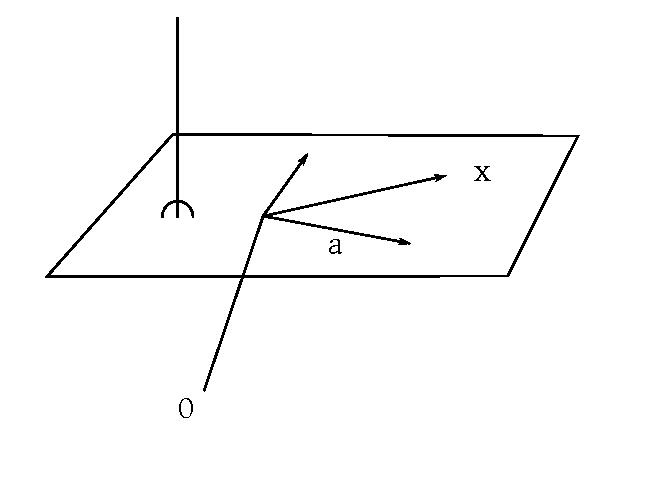
\includegraphics{img/05_application.pdf}
\end{example}

\subsection{Inner products and positive definiteness}
From now on $\mathbb K$ will be $\mathbb R$ or $\mathbb C$.

\begin{definition} % Definition 8.13
  An inner product on a vector space $V$ is a map
  \[ V \times V \to \mathbb K \qquad (x,y) \mapsto \angel{x,y} \]
  \begin{enumerate}
    \item $\angel{x+y, z} = \angel{x,z} + \angel{y,z} \quad \forall x,y,z \in V$
    \item $\angel{\lambda x, y} = \lambda \angel{x,y} \quad \forall \lambda \in \mathbb K \forall x,y \in V$
    \item $\angel{y,x} = \overline{\angel{x,y}} \quad \forall x,y \in V$
  \end{enumerate}
  where $\overline{\angel{x,y}}$ denotes the complex conjugate.

  \[
    \angel{x, \lambda y} \underbrace{=}_{\text{by (3)}} \overline{\angel{\lambda y, x}}
      \underbrace{=}_{\text{by (2)}} \overline{\lambda \angel{y, x}}
      = \overline{\lambda} \angel{x,y}
  \]

  The inner product is linear in $x$ and semi-linear in $y$, thus \emph{sesquilinear}\footnote{In Latin, sesqui means $1.5$}.

  In physics, the notation is different:
  \[ \braket{x|y} \qquad \braket{\lambda x|y} = \overline{\lambda} \braket{x|y} \qquad \braket{x|\lambda y} = \lambda \braket{x|y} \]
  \[ \langle x| \dots \text{ bra} \qquad |y\rangle \dots \text{ ket} \qquad \braket{x|y} \qquad \text{ bracket} \]

  The inner product is called \emph{positive-semidefinite}, if
  \[ \angel{x,x} \geq 0 \qquad \forall x \in X \]
  If $\angel{x,x} = 0 \iff x = 0$, then $\angel{\cdot,\cdot}$ is called \emph{positive definite}.
\end{definition}

\dateref{2018/04/09. Easter holidays finished}

\begin{lemma} % 8.14
  \begin{enumerate}
    \item $\angel{x, y + z} = \angel{x, y} + \angel{x, z}$
    \item $\angel{x, \lambda y} = \overline{\lambda} \cdot \angel{x, y}$
    \item $\angel{x, 0} = 0$
  \end{enumerate}
\end{lemma}

\index{Positive semidefinite inner product}
\index{Positive inner product}
\index{Negative definite inner product}
\index{Indefinite inner product}
\index{Hermitian form}
\index{Unitary product}
\begin{definition}
  An inner product is \emph{positive semidefinite}, if $\angel{x, x} \geq 0$.
  Is \emph{positive definite}, if $\angel{x, x} > 0$ for all $x \neq 0$.
  Is \emph{negative definite}, if $\angel{x, x} < 0$ for all $x \neq 0$.
  Is \emph{indefinite}, if neither positive nor negative semidefinite.

  A positive definite inner product is called \emph{scalar product}.
  A positive definite inner product is in \emph{Hermitian form}, if $\mathbb K = \mathbb C$.
  A positive definite inner product is also called \emph{unitary product}, if $\mathbb K = \mathbb C$.

  So quadratic form over $\mathbb R$ and Hermitian form over $\mathbb C$.
\end{definition}

\begin{Remark}
  For example, the expression $\angel{x, x} > 0$ requires that $x \in \mathbb R$,
  but we defined the inner product over $\mathbb C$ as well. In Euclidean spaces,
  $\angel{x, x} \in \mathbb R$ anyhow, but more generally, the condition should
  require the absolute value: $\card{\angel{x, x}} > 0$.
\end{Remark}

\begin{example} % 8.15
  \begin{itemize}
    \item The dot product over $\mathbb R^n$ or $\mathbb C^n$ is given by,
      \[
        V = \mathbb R^n: \quad
        \angel{\begin{pmatrix} x_1 \\ \vdots \\ x_n \end{pmatrix}, \begin{pmatrix} y_1 \\ \vdots \\ y_n \end{pmatrix}}
        = \sum_{i=1}^n x_i y_i
        \qquad
        V = \mathbb C^n: \quad
        \angel{\begin{pmatrix} x_1 \\ \vdots \\ x_n \end{pmatrix}, \begin{pmatrix} y_1 \\ \vdots \\ y_n \end{pmatrix}}
        = \sum_{i=1}^n x_i \overline{y_i}
      \] \[
        V = \mathbb C^n \implies \angel{x, x} = \sum_{i=1}^n x_i \overline{x_i} = \sum_{i=1}^n \card{x_i}^2 \geq 0
        \to \text{ positive semi-definite }
      \]

    \item
      Let $A \in \mathbb R^{n \times n}$.
      Let $x, y \in \mathbb R^n$.
      \begin{align*}
        \angel{x, y}_A &= x^t \cdot A \cdot y \qquad \text{ is bilinear} \\
          &= \sum_{i=1}^n x_i \sum_{j=1}^n a_{ij} y_j = \sum_{i,j=1}^n a_{ij} x_i y_j
      \end{align*}
      hence $\angel{x, y}_A = \angel{y, x}_A$.
      It must hold that
      \[ \sum_{i,j=1}^n a_{ij} x_i y_j = \sum_{i,j=1}^n a_{ij} y_i x_j \forall x,y \]
      We let $x = e_k$ and $y = e_l$.
      \[ \implies a_{kl} = a_{lk} \forall k,l \]
      Hence $A = A^T$. $A$ is symmetrical.

      Let $A \in \mathbb C^{n \times n}$. Let $x, y \in \mathbb C^n$.
      \[ \angel{x, y}_A = \sum_{i=1}^n \sum_{j=1}^n x_i a-{ij} \overline{y_j} \]
      \[ \angel{x,y}_A = \angel{y,x}_A \forall x,y \]
      \[ \iff A^T = \overline{A} \qquad \text{ is in Hermitian form} \]
      \[ a_{ji} = \overline{a_{ij}} \forall i ,j \]

    \item
      \[ V = C[a,b] = \set{f: [a,b] \to \mathbb K \text{ continuous}} \]
      \[ \angel{f,g} = \int_a^b f(t) \overline{g(t)} \, dt \qquad \text{ is a scalar product} \]
      \[ \angel{f,f} = \int_a^b \card{f(t)}^2 \, dt \geq 0 \]

    \item
      Consider $V = l_2$ ($\mathbb R^{\infty}$ would be too large) where $l_2 = \setdef{(x_n)_{n\in\mathbb N}}{x_n \in \mathbb R, \sum_{n=1}^\infty x_n^2 < \infty}$.
      \[ \angel{x, y} = \sum_{n=1}^\infty x_n y_n \qquad \text{ is a scalar product} \]
      Does it converge? This is not obvious.

      Fourier claimed that this example (4) and example (3) are the same.
      He claimed every function can be written as $f(x) = \sum_{n=0}^\infty a_n e^{inx}$.

      \[ x \cdot x = \angel{x, x} = \sum_{i=1}^n x_i^2 = \norm{x}^2 \]
  \end{itemize}
\end{example}

\index{Norm}
\begin{definition}
  Let $V$ be a vector space.
  A \emph{norm} on $V$ is a map $\norm{\cdot}: V \to [0,\infty[$
  such that
  \begin{enumerate}
    \item $\norm{x} \geq 0$ and $\norm{x} = 0 \iff x = 0$
    \item $\norm{\lambda \cdot x} = \card{\lambda} \cdot \norm{x} \qquad \forall \lambda \in K, \forall x \in V$
    \item $\norm{x + y} \leq \norm{x} + \norm{y}$ is the triangle inequality
  \end{enumerate}
\end{definition}

\begin{Remark}
  Every norm is a metric with $d(x,y) = \norm{x - y}$.

  $d$ is translation invariant. $d(x + x_0, y + x_0) = d(x, y)$.
  This is compatible to a vector space.

  In a black hole ($\to$ physics), you have a different metric in every point (Riemannian geometry): $\angel{x,y}_{A(x,y)}$.
\end{Remark}

\index{Euclidean norm}
\begin{example}
  Let $V = \mathbb R^n$.
  \begin{itemize}
    \item $\norm{x}_2 = \left(\sum_{i=1}^n x_i^2\right)$ is called \emph{Euclidean norm}.
    \item $\norm{x}_1 = \sum_{i=1}^n \card{x_i}$ is called \emph{$L^1$ norm} or \emph{Manhattan norm}.
    \item $\norm{x}_{\infty} = \max\setdef{\card{x_i}}{i = 1, \dots, n}$
  \end{itemize}
  Let $V = C[a,b]$.
  \[ \norm{f}_1 \coloneqq \int_a^b \card{f(t)} \, dt \]
  \[ \norm{f}_\infty \coloneqq \max_{t \in [\overline{a}, b]} \card{f(t)} \qquad \text{ is a $L^\infty$-norm} \]
  \[ \norm{f}_2 \coloneqq \left(\int \card{f(t)}^2 \, dt \right)^{\frac12} \]
  The $L^1$-norm, gives rise to the Lebesgue integral.
\end{example}

\begin{theorem} % 8.19
  \label{thm:t819}
  Let $\angel{\cdot,\cdot}$ be a scalar product in $V$ (hence, positive-definite inner product).
  Then $\norm{x} = \sqrt{\angel{x,x}}$ is a norm on $V$.
\end{theorem}

\begin{proof}
  \begin{itemize}
    \item $\norm{x} \geq 0, \norm{x} = 0 \iff \angel{x,x} = 0 \iff x = 0$
    \item $\norm{\lambda x} = \sqrt{\angel{\lambda x, \lambda x}} = \sqrt{\lambda \cdot \overline{\lambda} \cdot \angel{x,x}} = \sqrt{\lambda^2 \cdot \angel{x,x}} = \card{\lambda} \cdot \sqrt{\angel{x,x}}$
    \item Triangle inequality. We will prove this after proving the CBS inequality.
  \end{itemize}
\end{proof}

\subsection{Cauchy-Bunyakovsky-Schwarz inequality}

\begin{lemma}[Cauchy-Bunyakovsky-Schwarz inequality] % 8.20
  \label{thm:cbs}
  Cauchy (1789--1857) for $\mathbb R^n$,
  Bunyakovsky (1804--1889) for infinite dimensions,
  Schwarz (1843--1921) generically.

  \[ \card{\angel{x,y}} \leq \norm{x} \cdot \norm{y} \]

  Hence, $l^2$ if $\sum_{n=1}^\infty x_n^2 < \infty$ and $\sum_{n=1}^\infty y_n^2 < \infty$.
  $\angel{x,x} < \infty$ and $\angel{y,y} < \infty$.
  \[ \implies \sum x_n y_n \leq \sqrt{\sum x_n^2} \sqrt{\sum y_n^2} \]

  If $\card{\angel{x,y}} = \norm{x} \cdot \norm{y} \iff x,y \text{ are linear dependent}$.
\end{lemma}

\begin{proof}
  Now we can continue with part 3 of the proof of Theorem~\ref{thm:t819}.
  Triangle inequality:
  \begin{align*}
    \norm{x + y}^2 &= \angel{x + y, x + y} \\
      &= \angel{x,x} + \angel{x,y} + \angel{y,x} + \angel{y,y} \\
      &\leq \norm{x}^2 + 2 \card{\angel{x, y}} + \norm{y}^2 \\
      &\leq \norm{x}^2 + 2 \norm{x} \norm{y} + \norm{y}^2 \\
      &= \left(\norm x + \norm y\right)^2
  \end{align*}
\end{proof}

\begin{proof}[Proof of CBS inequality, Lemma~\ref{thm:cbs}] \hfill{}
  \begin{description}
    \item[Case 1: $y = 0$] trivial
    \item[Case 2: $y \neq 0$]
      Let $\lambda \in \mathbb K$ be arbitrary.
      \begin{align*}
        0 &\leq \angel{x - \lambda y, x - \lambda y} \\
          &= \angel{x, x} - \angel{x, \lambda y} - \angel{\lambda y, x} + \angel{\lambda y, \lambda y} \\
          &= \angel{x, x} - \overline{\lambda} \angel{x,y} - \lambda \angel{y,x} + \card{\lambda}^2 \angel{y,y} \\
        \intertext{
          This holds for all $\lambda$, hence also for $\lambda = \frac{\angel{x,y}}{\angel{y,y}}$.
          Because $y \neq 0 \implies \angel{y,y} > 0$, we can divide.
        }
          &= \angel{x,x} - \frac{\overline{\angel{x,y}}}{\angel{y,y}} \cdot \angel{x,y} - \frac{\angel{x,y}}{\angel{y,y}} \cdot \angel{y,x} + \frac{\card{\angel{x,y}}^2}{\angel{y,y}^2} \cdot \angel{y,y} \\
          &= \angel{x,x} - \frac{\card{\angel{x,y}}^2}{\angel{y,y}} - \frac{\card{\angel{x,y}}^2}{\angel{y,y}} + \frac{\card{\angel{x,y}}^2}{\angel{y,y}} \\
          &= \norm{x}^2 - \frac{\card{\angel{x,y}}^2}{\norm{y}^2} \\
          &\implies \norm{x}^2 \cdot \norm{y}^2 - \card{\angel{x,y}}^2 \geq 0
      \end{align*}
  \end{description}
\end{proof}

\begin{proof}[Alternative proof of CBS inequality in $\mathbb R^n$]
  \begin{align*}
    0 &\leq \sum_{i=1}^n \sum_{j=1}^n (x_i y_j - x_j y_i)^2 \\
      &= \sum_{i,j=1}^n \left(x_i^2 y_j^2 - 2 x_i y_j x_j y_i + x_j^2 y_i^2\right) \\
      &= \sum_{i,j}^n x_i^2 y_j^2 - 2 \sum_{i,j} x_i x_j y_i y_j + \sum_{i,j} x_j^2 y_i^2 \\
      &= 2 \sum_i x_i^2 \sum_j y_j^2 - 2 \sum_i x_i y_i \sum_j x_j y_j \\
      &= 2 \norm{x}^2 \norm{y}^2 - 2 \angel{x,y}^2 \\
      &\leadsto \norm{x}^2 \norm{y}^2 = \angel{x,y}^2 + \frac12 \sum_i \sum_j (x_i y_j - x_j y_i)^2
  \end{align*}
  So for $n=3$, $\norm{x}^2 \norm{y}^2 = \angel{x,y}^2 + \norm{x \times y}^2$.
  Hence, equality is given iff $x$ and $y$ are linear dependent.

  In the general case:
  If $\card{\angel{x,y}} = \norm{x} \cdot \norm{y}$.
  From the proof, it follows that
  $\exists \lambda: \angel{x - \lambda y, x - \lambda y} = 0$
  \[ \implies x - \lambda y = 0 \implies x,y \text{ are linear independent} \]
\end{proof}

\begin{theorem} % 8.21
  Let $V$ be a vector space over $\mathbb K = \mathbb R$ or $\mathbb C$.
  Let $B = \set{b_1, \dots, b_n}$ be a basis.
  $\angel{\cdot,\cdot}$ is an inner product.
  What does $\angel{\cdot,\cdot}$ look like in regards of the coordinate?

  There exists a unique matrix $A$ in Hermitian form (hence, $a_{ij} = \overline{a_{ji}}, A = \overline{A^T}$)
  such that $\forall x,y \in V: \angel{x,y} = \Phi_B(x)^T \cdot A \cdot \overline{\Phi_B(y)}$.
  If $\angel{\cdot,\cdot}$ is positive definite, $A$ is invertible.
\end{theorem}

\begin{Remark}
  \[ \angel{x,y} = \sum x_i \overline{y_i} \]
  corresponds to $A = I$.
  \[ x^T \cdot I \cdot \overline{y} = x^T \cdot \overline{y} \]

  How about $A = -I$.
  \[ \angel{x,y}_A = -\sum x_i \overline{y}_i \]
  This is not a scalar product (because of negative definiteness).
\end{Remark}

\begin{proof}
  Let $x = \sum_{i=1}^n \xi_i b_i, y = \sum_{j=1}^n \eta_j b_{j}$.
  \begin{align*}
    \angel{x,y} &= \angel{\sum_{i=1}^n \xi_i b_i, \sum_{j=1}^n \eta_j b_j}
      = \sum_{i=1}^n \xi_i \sum_{j=1}^n \overline{\eta_j} \underbrace{\angel{b_i, b_j}}_{\eqqcolon a_{ij} \text{ is unique } a_{ij} = \angel{b_i, b_j}} \\
      &= \sum_{i=1}^n \sum_{j=1}^n \xi_i a_{ij} \overline{\eta}_j
      = \xi^T \cdot A \cdot \overline{\eta}
      = \Phi_B(x)^T \cdot A \cdot \Phi_B(y) \\
    a_{ji} &= \angel{b_j, b_i} = \overline{\angel{b_i, b_j}} = \overline{a_{ij}}
  \end{align*}

  Show: If $\angel{\cdot,\cdot}$ is positive definite, then $A$ is invertible.
  It suffices to show that $\operatorname{ker}{A} = \set{0}$.

  Assume: $A \cdot \xi = 0 \implies \xi^T \cdot A \cdot \xi = 0$.
  Let $x = \sum_{i=1}^n \xi_i b_i$. $\angel{x,x} = 0 \implies x = 0 \implies \xi = \Phi_B(x) = 0$
\end{proof}

\index{Conjugate transpose}
\index{Self-adjoint matrix}
\index{Hermitian matrix}
\begin{definition}\hfill{} % 8.22
  \begin{itemize}
    \item 
      Let $A \in \mathbb C^{n \times n}$.
      The matrix $A^* \coloneqq \overline{A^T}$ ($(A^*)_{ij} = \overline{a_{ji}}$)
      is called \emph{conjugate transpose}.
    \item
      $A$ is called \emph{self-adjoint} if $A = A^*$ (dt. \foreignlanguage{german}{selbst-adjungiert}).
    \item
      If $\mathbb K = \mathbb R$ and $A = \overline{A}$, then $A$ is called \emph{symmetric}. \\
      If $\mathbb K = \mathbb C$ and $A = A^*$, then $A$ is called \emph{Hermitian}.
    \item
      $A = A^*$ is called (positive/negative) (semidefinite/definite) if the corresponding sesquilinear form satisfies
      \[ \angel{\xi, \eta}_A = \xi^T \cdot A \cdot \overline{\eta} \circ 0 \text{ where $\circ$ is one of } \geq, >, \leq \text{ or } < \text{ respectively} \]
      Thus $A$ is positive definite iff $\forall \xi \in \mathbb K^n: \angel{\xi, \eta}_A = \xi^T \cdot A \cdot \overline{\eta} \geq 0$
      %Hence, $\xi^T A \overline{\xi} \geq 0 \forall \xi \neq 0$ is positive definite, has the corresponding property or
      %$\xi^T A \overline{\xi} > 0 \forall \xi \neq$ is positive semidefinite, has the corresponding property.
  
      %$\xi^T A \overline{\xi} \leq 0 \forall \xi \neq$ is negative definite or
      %$\xi^T A \overline{\xi} < 0 \forall \xi \neq$ is negative semidefinite.
    \item If $\exists \xi: \xi^T A \overline{\xi} > 0$ and $\exists \eta: \eta^T A \overline{\eta} < 0$, then $A$ is called indefinite.
  \end{itemize}
\end{definition}

\dateref{2018/04/11}

Inner product: $\angel{x,y}$
\begin{itemize}
  \item $\forall x: \angel{x,x} \geq 0$ positive semi-definite
  \item $\forall x \neq 0: \angel{x,x} > 0$ positive definite
\end{itemize}
with respect to basis $b_1, \dots, b_n$.
\[ \angel{x,y} = \sum a_{ij} \xi_i \overline{\eta_j} \qquad a_{ij} = \angel{b_i, b_j} \]

\begin{Remark}
  $A = A^*$ is called \emph{positive semidefinite} if $A \geq 0$ if $\forall \xi: \xi^T A \overline{\xi} \geq 0$.

  $A = A^*$ is called \emph{positive definite} $\iff$ $A > 0 \iff \forall \xi \in \mathbb K^n\setminus \set{0}: \xi^T A \overline{\xi} > 0$
  with $\xi^T A \overline{\xi} = \sum_{i=1} \sum_{j=1} a_{ij} \xi_i \overline{\xi_j}$.
\end{Remark}

\begin{Example}
  \[ A = I > 0 \]
  \[ \xi^T I \overline{\xi} = \sum_{i=1}^n \xi_i \overline{\xi_i} = \sum \card{\xi_i}^2 > 0 \qquad \text{ if } \xi \neq 0 \]
  \[ A = -I < 0 \text{ is negative definite} \]
  \[
    A = \begin{bmatrix}
      1 &        &   &    &        & \\
        & \ddots &   &    &        & \\
        &        & 1 &    &        & \\
        &        &   & -1 &        & \\
        &        &   &    & \ddots & \\
        &        &   &    &        & -1
    \end{bmatrix}
  \]
  is indefinite:
  \[ e_1^T A e_1 > 0 \qquad e_n^T A e_n < 0 \]
\end{Example}

\begin{Remark}
  For a diagonal matrix
  \[ A = \begin{bmatrix} a_1 &  & 0 \\ & \ddots & \\ 0 &  & a_n \end{bmatrix} \]
  $A = A^* \iff a_i = \overline{a}_i$, hence for all $a_i \in \mathbb R$.

  For a diagonal matrix it holds that
  \begin{align*}
    A > 0 & \text{ if all } a_i > 0: \xi^T A \overline{\xi} = \sum_{i=1}^n a_i \card{\xi_i}^2 \geq 0 \\
    A \leq 0 & \text{ if all } a_i \geq 0 \text{ if } \xi^T A \overline{\xi} = 0 \implies \text{ all } a_i \cdot \card{\xi_i}^2 = 0 \\
    A < 0 & \text{ if all } a_i < 0 \\
    A \leq 0 & \text{ if all } a_i \leq 0 \\
    \text{indefinite} & \text{ if } \exists i: a_i > 0 \exists j: a_j < 0
  \end{align*}
\end{Remark}

\begin{Remark}
  Remember, that the rank of matrix satisfies:
  \[ \exists P,Q \in \operatorname{GL}(n): PAQ = \begin{pmatrix} 1 & & & \\ & 1 & & \\ & & \ddots & \\ & & & 0 \end{pmatrix} \]
  \[ A \sim PAQ \text{ is equivalent} \]
\end{Remark}

\subsection{Congruence of matrices}

\index{Congruence of matrices}
\begin{definition}[Congruence] % Definition 8.23
  Consider two self-adjoint matrices $A, B \in \mathbb K^{n \times n}$ are called congruent (denoted $A \hat= B$)
  if $\exists C \in \operatorname{GL}(n, \mathbb K)$ such that $C^* AC = B$.
\end{definition}

\begin{Remark}
  $C$ is invertible, hence $C^T$ is invertible.
  \[ (C^T)^{-1} = (C^{-1})^T \qquad (C^{-1})^T \cdot C^T = (C \cdot C^{-1})^T = I^T = I \]
  \[ (\overline{A}^{-1}) = \overline{A^{-1}} \]
  \[ (AB)^* = \overline{(AB)^T} = \overline{B^T A^T} = \overline{B^T} \cdot \overline{A^T} = B^* \cdot A^* \]

  $C^* AC$ is self-adjoint.
  \[ (C^* AC)^* = C^* \cdot A^* \cdot (C^*)^* = C^* \cdot A \cdot C \]
\end{Remark}

\begin{theorem} % Satz 8.24
  \label{thm:Herm}
  Every Hermitian matrix is congruent to a diagonal matrix $D$ of structure:
  \[ \operatorname{diag}(D) = (1, 1, \dots, 1, -1, \dots, -1, 0, \dots, 0) \]
\end{theorem}

\begin{proof}
  The proof is given by an algorithm.

  We construct matrix C inductively such that
  \[ C^* A C = \operatorname{diag}(\pm 1, \dots, 0) \]
  Consider $n = 1$.
  \[ A = [a_{11}] \]
  If $a_{11} = 0$ where $a_{11} \in \mathbb R$, we don't have to do anything.
  If $a_{11} \neq 0$ and $a_{11} \in \mathbb R$ (because $A$ is self-adjoint),
  \[ C = \left[\frac{1}{\sqrt{\card{a_{11}}}}\right] \]
  \[ C^* AC = \left[\frac{1}{\sqrt{\card{a_{11}}}} \cdot a_{11} \cdot \frac{1}{\sqrt{\card{a_{11}}}}\right] = \left[\operatorname{sign}(a_{11})\right] \]

  \begin{example} % 8.25
    \label{ex825}
    \[
      A = \begin{bmatrix}
        0 & 1 & i \\
        1 & 0 & 1 \\
        -i & 1 & 0
      \end{bmatrix}
    \]
  \end{example}

  \begin{Remark}
    It seems we need to take the absolute value in the complex numbers:
    Let $a = 3 + 4i$. $\card{a} = 5$.
    \[ C^* AC = \left[\frac1{\sqrt{\card{a_{11}}}} \cdot \card{a_{11}} \cdot \frac1{\sqrt{\card{a_{11}}}}\right] = \left[\frac1{\sqrt5} \cdot 5 \cdot \frac1{\sqrt{5}}\right] = [1] \]
  \end{Remark}

  Then $n-1 \to n$:
  \begin{description}
    \item[Case 1: $A = 0$] nothing to do.
    \item[Case 2: $a_{11} = 0$]
      \begin{description}
        \item[Case 2a:] 
          \[
            \exists j: a_{jj} \neq 0:
            \begin{bmatrix}
              0 & & & & \\
                & & a_{jj} & & \\
            \end{bmatrix}
          \]
          \[
            T_{(1,j)} = \begin{bmatrix}
              0 &   & & & & & & 1 \\
                & 1 & & & & & & \\
                &   & \ddots & & & & & \\
                &   &    & 1 & & & & \\
                &   &    & & 0 & & & \\
                &   &    & &   & 1 & & \\
                &   &    & &   &  & \ddots & \\
              1 &   &    & &   &  &  & 1 \\
            \end{bmatrix}
            = T^*_{(ij)}
          \]
          Permutation matrix that swaps 1 with $j$.

          \[
            T_{(1j)}^* A T_{(1j)} =
            \begin{bmatrix}
              a_{ji}  & \ldots & \ldots \\
              \vdots  & \ddots &   \\
              \vdots  &        & 0 \\
            \end{bmatrix}
          \]
          where $T_{(1j)}^*$ exchanges $j$-th and first row
          and $T_{(1j)}$ exchanges $j$-th and first column.
        \item[Case 2b]:
          all $a_{jj} = 0$. Choose $i,j$ such that $a_{ij} \neq 0$.
          Let $E_{ij}$ be a zero matrix with $1$ at row $i$ and column $j$.
          \[ C = I + E_{ij} e^{i\theta} \]
          where $\theta$ such that $a_{ij} = e^{i\theta} \card{a_{ij}}$.

          \begin{Example}
            $a_{12} \neq 0$
            \[
              C_1 = \begin{bmatrix}
                1 & 1 & \\
                  & 1 & \\
                  &   & 1
              \end{bmatrix}
            \] \[
              C_1^* A C_1
              = \begin{bmatrix}
                1 & 0 & 0 \\
                1 & 1 & 0 \\
                0 & 0 & 1
              \end{bmatrix} \cdot \begin{bmatrix} 
                0 & 1 & i \\
                1 & 0 & 1 \\
                -i & 1 & 0
              \end{bmatrix} \cdot \begin{bmatrix}
                1 & 1 & 0 \\
                0 & 1 & 0 \\
                0 & 0 & 1
              \end{bmatrix}
              = \begin{bmatrix}
                0 & 1 & i \\
                1 & 2 & 1+i \\
                -i & 1-i & 0
              \end{bmatrix}
            \]
          \end{Example}

          In the general case:
          \[ C^* AC = (I + E_{ji} e^{-i\theta}) A (I + E_{ij} e^{i\theta}) \]
          \begin{align*}
            (C^* AC)_{jj} &= \left(A + E_{ji} e^{-i\theta} A + AE_{ij} e^{+i\theta} + E_{ji} A E_{ij}\right)_{jj} \\
              &=
                \underbrace{a_{jj}}_{=0} +
                \underbrace{(E_{ji} e^{-i\theta} A)_{jj}}_{e^-i\theta a_{jj} = \card{a_{ij}}} +
                \underbrace{(AE_{ij} e^{+i\theta})_{jj}}_{a_{ji} e^{+i\theta} = \overline{a_{ij}} e^{i\theta} = \card{a_{ij}}} +
                \underbrace{a_{ii}}_{=0} \\
              &= 2 \card{a_{ij}}
          \end{align*}
          Case 2a is shown.

          \begin{Example}
            \[
              C_2 = \begin{bmatrix}
                0 & 1 & \\
                1 & 0 & \\
                  &   & 1
              \end{bmatrix} = T_{(12)}
            \]
          \end{Example}

          \[
            A_2 = C_2^* A_1 C_2 = \begin{bmatrix}
              0 & 1 & 0 \\
              1 & 0 & 0 \\
              0 & 0 & 1
            \end{bmatrix} \cdot \begin{bmatrix}
              0 & 1 & i \\
              1 & 2 & i+1 \\
              -i & 1-i & 0
            \end{bmatrix} \cdot \begin{bmatrix}
              0 & 1 & 0 \\
              1 & 0 & 0 \\
              0 & 0 & 1
            \end{bmatrix}
            = \begin{bmatrix}
              2 & 1 & 1+i \\
              1 & 0 & i \\
              1+i & -i & 0
            \end{bmatrix}
          \]
      \end{description}
    \item[Case 3]
      $a_{11} \neq 0$
      \[
        C = \begin{bmatrix}
          1 & -\frac{a_{12}}{a_{11}} & -\frac{a_{13}}{a_{11}} & \dots  & -\frac{a_{in}}{a_{11}} \\
            & 1                      &                 \ldots &     0  &         0 \\
            & \vdots                 & 1                      &        &         0 \\
            & 0                      &                        & \ddots &           \\
            & 0                      & 0                      & \ldots &         1 \\
        \end{bmatrix}
      \]

      \begin{Example}
        \[
          C_3 = \begin{bmatrix}
            1 & -\frac12 & -\frac{1+i}2 \\
              & 1        & \\
              &          & 1
          \end{bmatrix}
        \] \[
          A_3 = C_3^* A_2 C_3 = \begin{bmatrix}
            1 & 0 & 0 \\
            -\frac12 & 1 & 0 \\
            -\frac{1-i}{2} & 0 & 1
          \end{bmatrix} \cdot \begin{bmatrix}
            2 & 1 & 1+i \\
            1 & 0 & i \\
            1-i & -i & 0
          \end{bmatrix} \cdot \begin{bmatrix}
            1 & -\frac12 & -\frac{1+i}{2} \\
            0 & 1 & 0 \\
            0 & 0 & 1
          \end{bmatrix}
        \] \[
          \begin{bmatrix}
            2 & 1 & 1+i \\
            0 & -\frac12 & \frac12 (-i + i) \\
            0 & \frac12 (-1-i) & -1
          \end{bmatrix} \cdot \begin{bmatrix}
            2 & 0 & 0 \\
            0 & -\frac12 & \frac{-1+i}{2} \\
            0 & \frac{-1-i}{2} & -1
          \end{bmatrix}
        \]
      \end{Example}
      \[
        C^* AC = \begin{bmatrix}
          a_{11} & 0 & \ldots    & 0 \\
          0      &   &           &   \\
          \vdots &   & \tilde{A} &   \\
          0      &   &           & 
        \end{bmatrix}
      \] \[
        \tilde{A} \in \mathbb K^{(n-1) \times (n-1)}
      \] \[
        \tilde{A} = \tilde{A}^*
      \]

      \[
        C' = \begin{bmatrix}
          \frac{1}{\sqrt{\card{a_{11}}}} &  & & 0 \\
             & 1 & & \\
             &   & \ddots & \\
          0  &   &        & 1
        \end{bmatrix}
      \] \[
        (C')^* (C^* AC) C' = \begin{bmatrix}
          \frac{a_{11}}{\card{a_{11}}} & 0 &  & 0 \\
          0 & & & \\
          \vdots & & & \\
          0 & & & \tilde{A} \\
        \end{bmatrix}
        \text{ where } \frac{a_{11}}{\card{a_{11}}} = \pm 1
      \]
      Apply this algorithm to $\tilde{A}$.

      \begin{Example}[Part 4]
        \[ C_4 = \begin{bmatrix} \frac1{\sqrt2} & & \\ & 1 & \\ & & 1 \end{bmatrix} \]
        \[ A_4 = C_4^* A_3 C_4 = \begin{bmatrix}
          1 & 0 & 0 \\
          0 & -\frac12 & \frac{-1+i}{2} \\
          0 & \frac{-1-i}{2} & -1
          \end{bmatrix}
        \] \[
          \tilde A = \begin{bmatrix}
            -\frac12 & \frac{-1+i}{2} \\
            \frac{-1-i}{2} & -1
          \end{bmatrix}
        \] \[
          C_5 = \begin{bmatrix}
            1 & & \\
              & 1 & -1+i \\
              & 0 & 1
          \end{bmatrix}
        \] \[
          A_5 = C_5^* A_4 C_5 = \begin{bmatrix}
            1 & 0 & 0 \\
            0 & 1 & 0 \\
            0 & -1-i & 1
          \end{bmatrix} \cdot \begin{bmatrix}
            1 & 0 & 0 \\
            0 & -\frac12 & \frac{-1+i}{2} \\
            0 & \frac{-1-i}{2} & -1
          \end{bmatrix} \cdot \begin{bmatrix}
            1 & 0 & 0 \\
            0 & 1 & -1+i \\
            0 & 0 & 1
          \end{bmatrix}
        \] \[
          A_5 = \begin{bmatrix}
            1 & 0 & 0\\
            0 & -\frac12 & \frac{-1+i}{2} \\
            0 & 0 & 0
          \end{bmatrix} \cdot \begin{bmatrix}
            1 & 0 & 0 \\
            0 & 1 & -1+i \\
            0 & 0 & 1
          \end{bmatrix} = \begin{bmatrix}
            1 & 0 & 0 \\
            0 & -\frac12 & 0 \\
            0 & 0 & 0
          \end{bmatrix}
        \] \[
          C_6 = \begin{bmatrix}
            1 &  & \\
              & \sqrt2 & \\
              &  & 1
          \end{bmatrix}
        \] \[
          \sqrt2 = \frac{1}{\sqrt{\frac12}}
        \] \[
          C_6^* A_5 C_6 = \begin{bmatrix}
            1 &  & \\
              & -1 & \\
              &  & 0
          \end{bmatrix}
        \] \[
          C^*_6 \ldots C^*_2 C^*_1 A  C_1 C_2 \ldots C_6
          = \begin{bmatrix}
            1 &  & \\
              & -1 & \\
              &  & 0
          \end{bmatrix}
          \implies \text{ indefinite}
        \] \[
          C = C_1 C_2 \ldots C_6
        \] \[
          C^* = C^*_6 C^*_5 \ldots C^*_1
        \]
      \end{Example}
  \end{description}
\end{proof}

\begin{remark} % 8.26
  \begin{enumerate}
    \item If $A \geq 0$, $C$ arbitrary $\implies C^* AC \geq 0$.
      \[ \xi^T (C^* AC) \overline{\xi} = \underbrace{(\xi^T C^*)}_{\xi^T \overline{C^T} = \overline{\overline{\xi^T} C^T} = \overline{(C \cdot \overline{\xi})^T} = \overline{\eta^T}} A \underbrace{(C \overline{\xi})}_{\eta}
         = \overline{\eta}^T A \overline{\overline{\eta}} \geq 0
      \]
    \item If $A > 0$, $C$ invertible
      \[ \implies C^* AC > 0 \]
      \[ \text{if } \xi^T C^* AC \overline{\xi} = 0 \implies  \eta = C \overline{\xi} = 0 \text{ because } A > 0 \]
      \[ \implies \overline{\xi} = 0 \text{ because } C \text{ is invertible} \]

      \begin{corollary}
        If we apply the example~\ref{ex825} to $A>0$,
        \[
          C^* AC = \begin{bmatrix}
            \pm 1 &        &       &        &   & \\
                  & \ddots &       &        &   & \\
                  &        & \pm 1 &        &   & \\
                  &        &       & \ddots &   & \\
                  &        &       &        & 0 & \\
                  &        &       &        &   & \ddots
          \end{bmatrix}
          \text{ is still positive definite }
          \implies C^* AC = I
        \]
      \end{corollary}
  \end{enumerate}
\end{remark}

\begin{Person}
  James Joseph Sylvester (1814--1897)
\end{Person}

\begin{theorem}[Sylvester's law of inertia]
  Let $A \in \mathbb C^{n\times n}$ be Hermitian.
  $C \in \operatorname{GL}(n, \mathbb C)$ by the algorithm
  such that
  \[ C^* AC = \begin{bmatrix}
    \pm 1 &        &       &    &        &    &   &        & \\
          & \ddots &       &    &        &    &   &        & \\
          &        & \pm 1 &    &        &    &   &        & \\
          &        &       & -1 &        &    &   &        & \\
          &        &       &    & \ddots &    &   &        & \\
          &        &       &    &        & -1 &   &        & \\
          &        &       &    &        &    & 0 &        & \\
          &        &       &    &        &    &   & \ddots & \\
          &        &       &    &        &    &   &        & 0
    \end{bmatrix}
  \]
  Then the number of $+1$, $-1$ and zeros is uniquely determined
  (it does not depend on the order to the operands).
\end{theorem}

\begin{proof}
  $C$ is invertible, hence
  \[
    \rank(A) =
    \rank \begin{bmatrix}
       +1 &        &       &    &        &    &   &        & \\
          & \ddots &       &    &        &    &   &        & \\
          &        &    +1 &    &        &    &   &        & \\
          &        &       & -1 &        &    &   &        & \\
          &        &       &    & \ddots &    &   &        & \\
          &        &       &    &        & -1 &   &        & \\
          &        &       &    &        &    & 0 &        & \\
          &        &       &    &        &    &   & \ddots & \\
          &        &       &    &        &    &   &        & 0
    \end{bmatrix}
  \]
  Let $r$ be the number of $+1$ and $s$ be the number of $-1$.
  The number of $+1$ and $-1$ is uniquely determined.

  Hence, it suffices to show that the number $r$ of $+1$ is uniquely defined.

  Let $\tilde{C}$ be another matrix such that
  \[ \tilde C^* A \tilde C = \begin{bmatrix}
    \pm 1 &        &       &    &        &    &   &        & \\
          & \ddots &       &    &        &    &   &        & \\
          &        & \pm 1 &    &        &    &   &        & \\
          &        &       & -1 &        &    &   &        & \\
          &        &       &    & \ddots &    &   &        & \\
          &        &       &    &        & -1 &   &        & \\
          &        &       &    &        &    & 0 &        & \\
          &        &       &    &        &    &   & \ddots & \\
          &        &       &    &        &    &   &        & 0
    \end{bmatrix}
  \]
  with $\tilde r$ ones and $\tilde s$ minus ones.

  It suffices to show that $r \leq \tilde r$.
  We know $r+s = \tilde r + \tilde s$.

  $C$ is an invertible matrix, hence a change of basis.
  In this new basis $B' = \set{b_1, \dots, b_n}$, it holds that
  \[ x^* A x = \overline{x^T} A x = \overline{\Phi_B(x)^T} \cdot D \cdot \Phi_B(x) \]

  \[ A = (C^*)^{-1} D C^{-1} \]
  \[ \overline{x^T} A x = \overline{x^T} (C^*)^{-1} D \underbrace{C^{-1} x}_{\overline{C}^{-1} x} \]
  Equivalently, $\tilde C$ is a change of basis to basis $\tilde B$
  such that $x^* Ax = \Phi_{\tilde B}(x)^* \tilde D \tilde\Phi_{\tilde B}(x)$.
  For $x \in \mathcal L(\set{b_1, \dots, b_r}) \setminus \set{0}$,
  \[ \Phi_B(x) = \begin{pmatrix} \xi_1 \\ \vdots \\ \xi_r \\ 0 \\ \vdots \\ 0 \end{pmatrix} \]
  \[ \implies x^* A x = \Phi_B(x)^* D \Phi_B(x) \]
  \[
    = (\overline{\xi}_1, \dots, \overline{\xi}_r, 0, \dots, 0)
    \begin{bmatrix}
       +1 &        &       &    &        &    &   &        & \\
          & \ddots &       &    &        &    &   &        & \\
          &        &    +1 &    &        &    &   &        & \\
          &        &       & -1 &        &    &   &        & \\
          &        &       &    & \ddots &    &   &        & \\
          &        &       &    &        & -1 &   &        & \\
          &        &       &    &        &    & 0 &        & \\
          &        &       &    &        &    &   & \ddots & \\
          &        &       &    &        &    &   &        & 0
    \end{bmatrix} \cdot
    \begin{pmatrix}
      \xi_1 \\ \vdots \\ \xi_r \\ 0 \\ \vdots \\ 0
    \end{pmatrix}
    = \sum_{i=1}^r \card{\xi_i}^2 > 0
  \]
  On the other hand, $\forall x \in \mathcal L(\tilde b_{\tilde r + 1}, \dots, \tilde b_n)$.
  \[
    \Phi_{\tilde B}(x) =
      \begin{pmatrix}
        0 \\ \vdots \\ 0 \\
        \tilde \xi_{\tilde r+1} \\
        \vdots \\ \tilde \xi_n
      \end{pmatrix}
  \] \[
    x^* Ax = \Phi_{\tilde B}(x)^* \tilde D \Phi_{\tilde B}(x)
  \] \[
    = (0, \dots, 0, \tilde \xi_{\tilde r + 1}, \dots, \tilde \xi_n)
    \begin{bmatrix}
       +1 &        &       &    &        &    &   &        & \\
          & \ddots &       &    &        &    &   &        & \\
          &        &    +1 &    &        &    &   &        & \\
          &        &       & -1 &        &    &   &        & \\
          &        &       &    & \ddots &    &   &        & \\
          &        &       &    &        & -1 &   &        & \\
          &        &       &    &        &    & 0 &        & \\
          &        &       &    &        &    &   & \ddots & \\
          &        &       &    &        &    &   &        & 0
    \end{bmatrix} \cdot \begin{bmatrix}
      0 \\ \vdots \\ 0 \\ \tilde \xi_{\tilde r+1} \\ \vdots \\ \tilde \xi_n
    \end{bmatrix} \leq 0
  \] \[
    \implies \mathcal L(b_1, \dots, b_r) \cap \mathcal L(\tilde b_{\tilde r+1}, \dots, \tilde b_n) = \set{0}
  \] \[
    \text{dimension } r + (n - \tilde r) \leq n \implies r \leq \tilde r
  \]
\end{proof}

\dateref{2018/04/16}

\[ A = A* \]
Conjugate complex. The important question: When does it hold that
\[ A > 0 \]
Hence
\[ \forall x \in \mathbb C^n: x^* A x \geq 0 \]
\[ A > 0 \text{ if } x^* A x > 0 \forall x \neq 0 \]
\[ (x^*)_i = \overline{x}_i \]
\[ \exists C \in \operatorname{GL}(n, \mathbb C) \text{ such that } \]
\[ C^* AC \underbrace{=}_{\text{congruence}} \begin{bmatrix}
     +1 &        &       &    &        &    &   &        & \\
        & \ddots &       &    &        &    &   &        & \\
        &        &    +1 &    &        &    &   &        & \\
        &        &       & -1 &        &    &   &        & \\
        &        &       &    & \ddots &    &   &        & \\
        &        &       &    &        & -1 &   &        & \\
        &        &       &    &        &    & 0 &        & \\
        &        &       &    &        &    &   & \ddots & \\
        &        &       &    &        &    &   &        & 0
  \end{bmatrix}
\]
where the number of $+1$ is $r$ (see Sylvester's Law of inertia).

\begin{definition} % Definition 8.28
  If $A = A*$ is congruent to
  \[
    \begin{bmatrix}
     +1 &        &       &    &        &    &   &        & \\
        & \ddots &       &    &        &    &   &        & \\
        &        &    +1 &    &        &    &   &        & \\
        &        &       & -1 &        &    &   &        & \\
        &        &       &    & \ddots &    &   &        & \\
        &        &       &    &        & -1 &   &        & \\
        &        &       &    &        &    & 0 &        & \\
        &        &       &    &        &    &   & \ddots & \\
        &        &       &    &        &    &   &        & 0
    \end{bmatrix}
  \]
  with $r$ occuring $+1$s and $s$ occuring $-1$s.

  Then $\operatorname{ind}(A) \coloneqq r$ is called \emph{index of A}.
  $\sign(A) \coloneqq r - s$ is called \emph{signature of A}.
\end{definition}

\begin{corollary} % Folgerungen 8.29
  \label{cor829}
  \begin{enumerate}
    \item $A > 0 \iff A \hat= I \iff \operatorname{ind}(A) = n$
    \item $A \geq 0 \iff \operatorname{ind}(A) = \sign(A) = \rank(A)$
    \item $A \hat= B \iff \operatorname{ind}(A) = \operatorname{ind}(B) \land \sign(A) = \sign(B)$
  \end{enumerate}
  It is left as an exercise to the reader that congruence is an equivalence relation.
  \begin{enumerate}
    \item $I \cdot A \cdot I = A$
    \item $A \hat= B \implies C^* A C = B \implies A = (C^*)^{-1} BC^{-1} = (C^{-1})* BC^{-1} \implies B \hat= A$
    \item $C^*_1 A_1 C_1 = A_2 \land C_2^* A_2 C_2 = A_3 \implies \underbrace{C_2^* C_1^* A_1 C_1 C_2}_{= (C_1 C_2)^* A_1 (C_1 C_2) \implies A_1 \hat= A_3} = A_3$
  \end{enumerate}
  Furthermore it will be shown in the practicals that $A > 0 \iff \exists C A = C^* C$
\end{corollary}

\begin{Remark}[Idea]
  \[
    \det(C^* A C) = \det\begin{bmatrix}
     +1 &        &       &    &        &    &   &        & \\
        & \ddots &       &    &        &    &   &        & \\
        &        &    +1 &    &        &    &   &        & \\
        &        &       & -1 &        &    &   &        & \\
        &        &       &    & \ddots &    &   &        & \\
        &        &       &    &        & -1 &   &        & \\
        &        &       &    &        &    & 0 &        & \\
        &        &       &    &        &    &   & \ddots & \\
        &        &       &    &        &    &   &        & 0
    \end{bmatrix}
  \] \[
    \det(C^*) \det(A) \det(C) = \begin{cases}
      0 & \text{ if } \rank(A) < n \\
      (-1)^{\text{number of } -1}
    \end{cases}
  \]
  \[ \overline{\det(C)} \det(A) \det(C) \]
  If $A > 0$,
  \[ \card{\det(C)}^2 \cdot \det(A) = 1 \implies \det(A) > 0 \]
\end{Remark}

\begin{lemma}
  \begin{enumerate}
    \item $\det(C^*) = \overline{\det(C)}$
    \item $A = A^* \implies \det(A) \in \mathbb R$
    \item $A = A^*, B = B^*, A \hat= B \implies \sign{\det(A)} = \sign{\det(B)}$
    \item $A > 0 \implies \det(A) > 0$
      but not the other way around:
      \[ \det\begin{bmatrix} -1 & \\ & -1 \end{bmatrix} = 1 \]
  \end{enumerate}
\end{lemma}

\begin{proof}
  \begin{enumerate}
    \item
      \[ \det(C^*) = \sum_{\sigma \in \Sigma_n} (-1)^\sigma \underbrace{\underbrace{(C^*)_{1 \sigma(1)}}_{\overline{C_{\sigma(1) 1}}} \ldots \underbrace{(C^*)_{n \sigma(n)}}_{\overline{C_{\sigma(n) n}}}}_{= \overline{\sum_{\sigma} (-1)^\sigma C_{\sigma(1) 1} \ldots C_{\sigma(n) n} = \overline{\det(C)} }} \]
    \item immediate
    \item $A \hat B \implies C^* AC = B$
      \[ \det(C^* AC) = \det(B) \]
      \[ \underbrace{\card{\det(C)}^2}_{>0} \cdot \det(A) = \det(B) \]
    \item $A \hat= I \implies \sign{\det(A)} = \sign{\det(I)} = 1$
  \end{enumerate}
\end{proof}

\index{Minor of a square matrix}
\begin{definition} % Definition 8.31
  Let $A \in \mathbb K^{m \times n}, r \leq \min\set{m,n}$.
  \[ I = \underbrace{\set{i_1 < \ldots < i_r}}_{\subseteq \set{1, \ldots, m}} \qquad J = \underbrace{\set{j_1 < \ldots < j_r}}_{\subseteq \set{1, \ldots, n}} \]
  Then
  \[
    \left[A\right]_{I,J} =
    \begin{vmatrix}
      a_{i_1 j_1} & a_{i_1 j_2} & \ldots & a_{i_1 j_r} \\
      a_{i_2 j_1} & a_{i_2 j_2} & \ldots & a_{i_2 j_r} \\
      \vdots & \vdots & \ddots & \vdots \\
      a_{i_r j_1} & a_{i_r j_2} & \ldots & a_{i_r j_r}
    \end{vmatrix}
  \]
  is called \emph{minor of A}.
\end{definition}

\begin{Example}
  Let $r = 1$, $I = \set{i_1}$, $J = \set{j_1}$, $[A]_{\set{i_1}, \set{j_1}}  = a_{i_1 j_1}$.
\end{Example}

\begin{definition}
  If $m=n$ with $I = \set{1, \ldots, r}$ and $J = \set{1, \ldots, r}$, then
  \[
    \begin{vmatrix}
      a_{11} & a_{12} & \ldots & a_{1r} \\
      \vdots & \vdots & \ddots & \vdots \\
      a_{r1} & a_{r2} & \ldots & a_{rr}
    \end{vmatrix}
  \]
  the first minor of $A$ (\foreignlanguage{german}{Hauptminoren}).
  \[ A < 0 \iff (-A) > 0 \]
  \[ \det(\lambda A) = \lambda^* \det(A) \]
\end{definition}

\begin{theorem}[dt.~\foreignlanguage{german}{Hauptminorenkriterium}] % Satz 8.32
  Let $A = A^*$, then it holds that
  \begin{enumerate}
    \item $A > 0 \iff$ all first minors satisfy $\det(A_r) > 0$
    \item $A < 0 \iff (-1)^r \det(A_r) > 0 \forall r \in \set{1, \ldots, n}$
  \end{enumerate}
\end{theorem}

\begin{proof}\hfill{}
  \begin{description}
    \item[Direction $\implies$:] 
      For $r = n$: $\det(A_r) = \det(A) > 0$.
      It suffices to show: submatrices
      \[ A_r = \begin{bmatrix} a_{11} & a_{12} & \ldots & a_{1r} \\ \vdots & & & \\ a_{r1} &  & & a_{rr} \end{bmatrix} \]
      are positive definite.
      Hence, $\forall x \in \mathbb C^r$ with $x \neq 0: x^* A_r x > 0$.

      \[ x \in \mathbb C^r \setminus \set{0}: x^* A_r x = \left[x^* \underbrace{0}_{n - r}\right] \cdot A \cdot \begin{bmatrix} x \\ 0 \end{bmatrix} > 0 \]
      \[ = [x^* 0] \begin{bmatrix} A_r & & & * \\ & & & \vdots \\ & & & * \\ * & \ldots & * & * \end{bmatrix} \begin{bmatrix} x \\ 0\end{bmatrix} \]
      Remark: \emph{every submatrix}
      $\begin{bmatrix} a_{i_1 i_1} & \ldots & a_{i_1 i_r} \\ \vdots & \ddots & \vdots \\ a_{i_r i_1} & \ldots & a_{i_r i_r} \end{bmatrix}$
      of a positive definite matrix is positive definite.
    \item[Direction $\impliedby$:]
      Assume all first minors $\det(A_r) > 0$.

      We use complete induction:
      \begin{description}
        \item[Let $n=1$ and $r=1$:]
          $A = [a_{11}]$ and $\det(A_1) = a_{11}$.
          $A > 0 \iff a_{11} > 0$.
        \item[Consider $n \to n+1$:]
          Assume all first minors are greater $0$.
          Then all first minors of matrix $A_{n-1}$ are greater $0$ by induction hypothesis.
          \[ \text{Theorem~\ref{thm:Herm}} \implies \exists C: C^* A_{n - 1} C = I_{n-1} \]

          \begin{align*}
            A' &= \begin{bmatrix}
                      &       &   & 0 \\
                      & C^*   &   & \vdots \\
                      &       &   & 0 \\
                    0 & \dots & 0 & 1
                  \end{bmatrix}
                  A
                  \begin{bmatrix}
                      &       &   & 0 \\
                      & C     &   & \vdots \\
                      &       &   & 0 \\
                    0 & \dots & 0 & 1
                  \end{bmatrix} \\
                  &= \begin{bmatrix}
                      &       &   & 0 \\
                      & C^*   &   & \vdots \\
                      &       &   & 0 \\
                    0 & \dots & 0 & 1
                  \end{bmatrix} \begin{bmatrix}
                      & & & a_{1, n} \\
                      & A_{n-1} & & \vdots \\
                      & & & a_{n-1,n} \\ \\
                    \overline{a_{1,n}} & \ldots & \overline{a_{n,n-1}} & a_{n,n}
                  \end{bmatrix} \begin{bmatrix}
                      &       &   & 0 \\
                      & C     &   & \vdots \\
                      &       &   & 0 \\
                    0 & \dots & 0 & 1
                  \end{bmatrix} \\
                  &= \begin{bmatrix}
                      & & & a_{1, n} \\
                      & I & & \vdots \\
                      & & & a_{n-1,n} \\ \\
                    \overline{a_{1,n}} & \ldots & \overline{a_{n,n-1}} & a_{n,n}
                  \end{bmatrix} \\
            C' &= \begin{bmatrix}
                    1 &        & 0 & -a_{1,n} \\
                      & \ddots &   & \vdots \\
                    0 &        & 1 & -a_{n-1,n} \\
                    0 & \dots  & 0 & 1 \\
                  \end{bmatrix}
                  = \left[
                    \begin{array}{c|c}
                      I & -b \\
                      \hline
                      0 & 1
                    \end{array}
                  \right]
                  \text{ with }
                  b = \begin{bmatrix} a_{11} \\ a_{21} \\ \vdots \\ a_{n-1,n} \end{bmatrix} \\
            (C')^* A'C' &= \left[
                    \begin{array}{c|c}
                      I & 0 \\
                      \hline
                      -b^* & 1
                    \end{array}
                  \right] \left[
                    \begin{array}{c|c}
                      I & b \\
                      \hline
                      b^* & a_{n,n}
                    \end{array}
                  \right] \left[
                    \begin{array}{c|c}
                      I & -b \\
                      \hline
                      0 & 1
                    \end{array}
                  \right] \\
              &= \left[
                    \begin{array}{c|c}
                      I & b \\
                      \hline
                      -b^* & -b^* b + a_{nn}
                    \end{array}
                  \right] \left[
                    \begin{array}{c|c}
                      I & -b \\
                      \hline
                      0 & 1
                    \end{array}
                  \right] \\
              &= \left[
                    \begin{array}{c|c}
                      I & 0 \\
                      \hline
                      0 & -b^* b + a_{nn}
                    \end{array}
                  \right] \\
          \end{align*}

          Hence
          \begin{itemize}
            \item $A \hat= A' \hat= \begin{bmatrix} I & 0 \\ 0 & -b^* b + a_n \end{bmatrix}$
            \item $\exists C'' = \begin{bmatrix} C & 0 \\ 0 & 1 \end{bmatrix} \cdot C'$ such that
              $
                (C'')^* AC'' = \left[
                  \begin{array}{c|c}
                    I & 0 \\
                    \hline
                    0 & a_{n,n} - b^* b
                  \end{array}
                \right]
              $
            \item 
              $
                \det(A) \cdot \card{\det(C'')}^2 = \det\begin{bmatrix}
                  I & 0 \\
                  0 & a_{n,n} - b^* b
                \end{bmatrix} = a_{n,n} - b^* b$
              \[
                \implies a_{n,n} - b^* b > 0
                \qquad
                \implies \begin{bmatrix}
                  I & 0 \\
                  0 & -b^* b + a_{nn}
                \end{bmatrix}
                \text{ is positive definite}
              \]
          \end{itemize}
      \end{description}
  \end{description}
\end{proof}

Back to the scalar product:

\begin{Person}
  David Hilbert (1862--1943)
\end{Person}

\index{Euclidean space}
\index{Unitary space}
\begin{definition} % 8.33
  \begin{enumerate}
    \item
      \begin{enumerate}
        \item A vector space with a positive definite inner product
          is called \emph{Euclidean space} ($K = \mathbb R, \dim < \infty$)
          or \emph{unitary space} ($K = \mathbb C$)
        \item Hilbert space if $\dim = \infty$.
      \end{enumerate}

      \[ \norm{v} = \sqrt{\ip vv} \]
      \[ \norm{\lambda v} = \card{\lambda} \cdot \norm{v} \]
      in $\mathbb R^2$: $\ip ab = \norm{a} \norm{b} \cos{\varphi}$
    \item An element $v \in V$ is called \emph{normed} if $\norm{v} = 1$
      (if not, then $\frac{v}{\norm{v}}$ is normed)
    \item
      Let $v, w \in V \setminus \set{0}$. Then the angle spanned between $v$ and $w$ is the angled $\varphi \in [0, \pi]$
      such that $\cos{\varphi} = \frac{\Re{\ip vw}}{\norm{v} \norm{w}}$
    \item Two vectors $v, w \in V$ are orthogonal ($v \bot w$)
      if $\ip vw = 0$ (hence $\varphi = \frac\pi2$)
  \end{enumerate}
\end{definition}

\begin{theorem} % 8.34
  \label{thm834}
  \begin{enumerate}
    \item $\norm{v + w}^2 = \norm{v}^2 + \norm{w}^2 + 2 \norm v \norm w \cos{\varphi}$ (Law of cosines)
    \item if $v \bot w$: $\norm {v + w}^2 = \norm{v}^2 + \norm{w}^2$ (Pythagorean Theorem)
    \item $\norm{v + w}^2 + \norm{v - w}^2 = 2 (\norm{v}^2 + \norm{w}^2)$ (Parallelogram Law)
  \end{enumerate}

  \begin{figure}[!ht]
    \begin{center}
      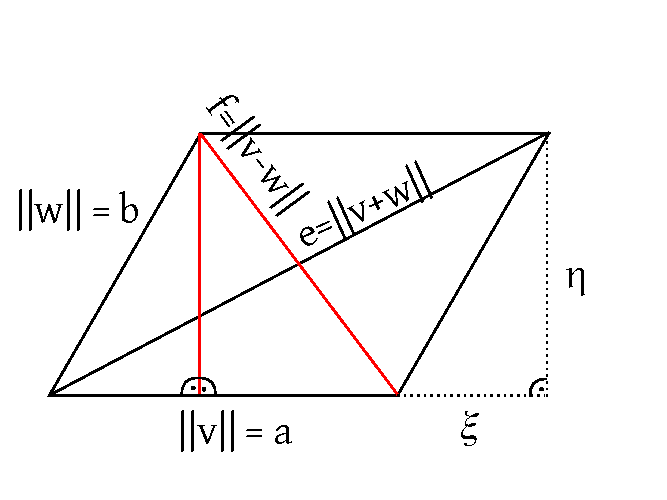
\includegraphics{img/06_geometrical_proof.pdf}
      \caption{Geometrical proof of Theorem~\ref{thm834}}
    \end{center}
  \end{figure}

  \[ e^2 + f^2 = 2 (a^2 + b^2) \]
  \[ e^2 = (a + \xi)^2 + \eta^2 \]
  \[ f^2 = (a - \xi)^2 + \eta^2 \]
  \[ e^2 + f^2 = (a + \xi)^2 + (a - \xi)^2 + 2\eta^2 \]
  \[ = a^2 + \xi^2 + a^2 + \xi^2 + 2\eta^2 = 2a^2 + 2b^2 \]
\end{theorem}

\begin{proof}
  \begin{enumerate}
    \item Show the Law of Cosines:
      \begin{align*}
        \norm{v + w}^2 &= \ip{v + w}{v + w} = \ip vv + \ip vw + \ip wv + \ip ww \\
          &= \norm{v}^2 + \ip vw + \overline{\ip vw} + \norm{w}^2 \\
          &= \norm{v}^2 + 2 \underbrace{\Re\ip vw}_{\cos\varphi \cdot \norm v \cdot \norm w} + \norm{w}^2
      \end{align*}
    \item Show the Pythagorean theorem: immediate, $\ip vw = 0$
    \item Show the Parallelogram law:
      \begin{align*}
        \norm{v + w}^2 + \norm{v - w}^2 &= {\norm v}^2 + \norm{w}^2 + 2 \Re\ip vw + \norm{v}^2 + \norm{-w}^2 + 2\Re\ip v{-w} \\
          &= 2 \norm{v}^2 + 2 \norm{w}^2 + 0
      \end{align*}
  \end{enumerate}
  Other norms:
  \[ \norm{\begin{bmatrix} x_1 \\ \vdots \\ x_n \end{bmatrix}}_1 = \sum_{1}^n \card{x_i} \qquad
     \norm{\begin{bmatrix} x_1 \\ \vdots \\ x_n \end{bmatrix}}_\infty = \max \card{x_i} \]
\end{proof}

\begin{remark} % 8.35
  You can show (von Neumann did):
  A norm on $\mathbb R^n$ satisfies the Parallelogram Law
  iff $\exists$ a scalar product on $\mathbb R^n$ such that $\norm v = \sqrt{\ip vv}$
\end{remark}

\index{Orthonormal}
\index{Orthonormal basis}
\begin{definition} % 8.36
  Let $(v, \ip{\cdot}{\cdot})$ be a vector space with scalar product.
  A family $(v_i)_{i \in I} \subseteq V$ is called
  \begin{description}
    \item[orthogonal] if $\forall i \neq j: \ip{v_i}{v_j} = 0$
    \item[orthonormal] if additionally $\norm{v_i} = 1 \forall i$ \\
      hence $\forall i,j: \ip{v_i}{v_j} = \delta_{ij}$
    \item[orthonormal basis] if they are orthonormal and give a basis of $V$.
  \end{description}
\end{definition}

\begin{example} % 8.37
  \begin{enumerate}
    \item Canonical basis in $\mathbb R^n$ in regards of the standard scalar product
      \[ \ip{e_i}{e_j} = \delta_{ij} \]
    \item Fourier $\set{\sqrt 2 \sin{2\pi x}, \sqrt2 \sin{4\pi x}, \ldots, \sqrt2 \sin(2k \pi x), \ldots}$ with $k \in \mathbb N$
      union with $\set{\sqrt2 \cos{2\pi x}, \sqrt2 \cos{4\pi x}, \ldots} \cup \set{\mathfrak 1}$
      on $C[0,1]$.
      \[ \ip fg = \int_0^1 f(x) g(x) \, dx \]
      And this is wrong unless we redefine the term basis (not every function is built using the sine/cosine).
      A basis here is every function:
      \[ f(x) = \sum_{k=0}^\infty a_k \cos(2k \pi x) + \sum_{k=1}^\infty b_k \sin(2k \pi 2) \]
      And this is wrong as well unless we define equality more precisely (in the usual sense, it is wrong).
      Lebesgue did this later.
  \end{enumerate}
\end{example}

\begin{Remark}
  For JPEG compression, Fourier transformation is applied. Hence, we consider
  the music (amplitudes) as $f$ and
  \[ f(x) = \sum_{k=0}^n a_k \cos{2k \pi x} + \sum_{k=1}^n b_k \sin{2k \pi 2} \]
  with $n$ finite.
\end{Remark}

\begin{theorem} % 8.38
  \label{thm838}
  Let $(v_i)_{i \in I} \subseteq V$, $v_i \neq 0 \forall i$
  \begin{enumerate}
    \item $(v_i)_{i \in I}$ orthogonal $\iff \left(\frac{v_i}{\norm{v_i}}\right)_{i \in I}$ is orthonormal
    \item $(v_i)_{i \in I}$ is orthogonal, then $(v_i)_{i \in I}$ is linear independent.
  \end{enumerate}
\end{theorem}

\dateref{2018/04/18}

%Revision:
%\[ \cos\varphi = \frac{\ip vw}{\norm{v} \norm{w}} \]
%\[ v \bot w \iff \ip vw = 0 \]
%$(v_i)_{i \in I}$ orthogonal if $\ip{v_i}{v_j} = 0 \forall i \neq j$ \\
%orthonormal: $\ip{v_i}{v_j} = \delta_{ij}$.

\begin{proof}[Proof of Theorem~\ref{thm838}]
  Let $\sum_{k=1}^n \lambda_k v_{i_k} = 0$.
  \[ \implies 0 = \angel{\sum_{k=1}^n \lambda \cdot v_{i_k}, v_i} = \sum_{k=1}^n \lambda_k \angel{v_{i_k}, v_i} \]
  $\forall l \in \set{1, \ldots, n}:$ Let $i = i_l$.
  \[
    i_l
      = \sum_{k=1}^n \lambda_k \underbrace{\angel{v_{i_k}, v_{i_l}}}_{= \begin{cases} 0 & i_k \neq i_l \\ \norm{v_{i_l}}^2 & i_k = i_l \end{cases}}
      = \lambda_l \cdot \norm{v_{i_l}}^2 \implies \lambda_l = 0 \]
\end{proof}

\begin{theorem} % 8.39
  Let $B = (b_1, \ldots, b_n)$ be an orthonormal basis of a finite dimensional vector space over $\mathbb K$.
  For $v \in V$, let $\Phi_B(v) = \begin{pmatrix} \lambda_1 \\ \vdots \\ \lambda_n \end{pmatrix}$.
  For $w \in V$, let $\Phi_B(w) = \begin{pmatrix} \mu_1 \\ \vdots \\ \mu_n \end{pmatrix}$.
  \begin{enumerate}
    \item $\lambda_i = \ip{v}{b_i}$
    \item $\ip vw = \sum_{i=1}^n \lambda_i \overline{\mu_i}$
  \end{enumerate}
\end{theorem}

\begin{proof}
  \begin{enumerate}
    \item
      \begin{align*}
        \ip{v}{b_i} &= \ip{\sum_{j=1}^n \lambda_j b_j}{b_i} 
                    = \sum_{j=1}^n \lambda_j \cdot \underbrace{\ip{b_j}{b_i}}_{= \delta_{ji}}
                    = \lambda_i
      \end{align*}
    \item
      \begin{align*}
        \ip vw &= \ip{\sum_{i=1}^n \lambda_i b_i}{\sum_{j=1}^n \mu_j b_j}
               = \sum_{i=1}^n \lambda_i \sum_{j=1}^n \overline{\mu_j} \underbrace{\ip{b_i}{b_j}}_{\delta_{ij}}
               = \sum_{i=1}^n \lambda_i \cdot \overline{\mu_i}
      \end{align*}
      Compare: $B$ is an arbitrary basis:
      \[ \ip vw = \Phi_B(v)^T \cdot A \cdot \overline{\Phi_B(w)} \]
      \[ a_{ij} = \ip{b_i}{b_j} = \delta_{ij} \]
      \[ A = I \]
      \[ \to \ip vw = \Phi_B(v)^T \cdot \overline{\Phi_B(w)} \]
  \end{enumerate}
\end{proof}

\index{Orthogonal complement}
\begin{definition}
  Let $V$ be a vector space with a scalar product.
  Let $v \in V$, then
  \[ v^\bot = \setdef{w \in V}{\ip vw = 0} \]
  For $M \subseteq V: M^\bot = \setdef{w \in V}{\forall u \in M: \ip uw = 0}$
  is called \emph{orthogonal complement of $v$} or \emph{orthogonal complement of $M$}.
\end{definition}

Compare with Figure~\ref{orthocomp}.
\begin{figure}[!ht]
  \begin{center}
    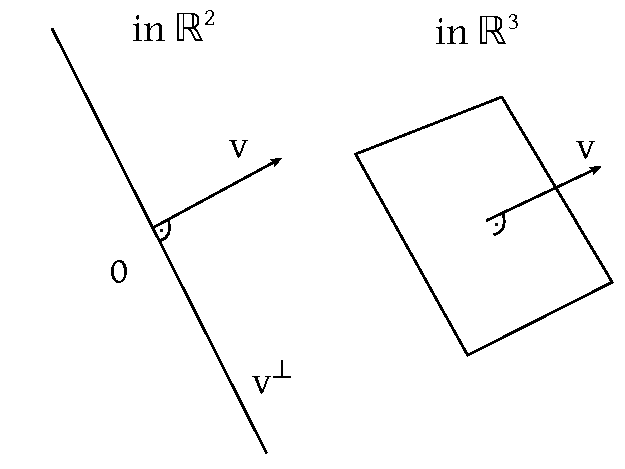
\includegraphics{img/07_orthogonal_complement.pdf}
    \caption{Orthogonal complement}
    \label{orthocomp}
  \end{center}
\end{figure}

In $\mathbb R^n$:
\[ \setdef{w}{\ip vw = 0} = \setdef{\begin{pmatrix} x_1 \\ \vdots \\ x_n \end{pmatrix}}{\sum_{1}^n a_i x_i = 0} \quad \text{ if } v = \begin{pmatrix} a_1 \\ \vdots \\ a_n \end{pmatrix} \]

\begin{theorem} % Theorem 8.41
  \label{thm841}
  Let $V$ be a vector space with scalar product. $M, N \subseteq V$ are partitions.
  \begin{enumerate}
    \item $M^\bot$ is a subspace.
    \item $M \subseteq N \implies N^\bot \subseteq M^\bot$ \\
      $(M_1 \cup M_2)^\bot = M_1^\bot \cap M_2^\bot$
    \item $\set{0}^\bot = V$
    \item $V^\bot = \set{0}$
    \item $M \cap M^\bot \subseteq \set{0}$
    \item $M^\bot = \mathcal L(M)^\bot$
    \item $M \subseteq (M^\bot)^\bot$
  \end{enumerate}
\end{theorem}

\begin{proof}
  \begin{enumerate}
    \item
      \begin{align*}
        v^\bot &= \setdef{w \in V}{\ip vw = 0} \\
          T_v: & V \to \mathbb K \text{ (linear functional)} \\
               & w \mapsto \ip wv
      \end{align*}
      \[ v^\bot = \setdef{w}{T_v(w) = 0} = \ker(T_v) \text{ is a subspace } \]
      % the kernel of a linear map is a subspace
      \[ M^\bot = \bigcap_{v \in M} v^\bot = \bigcap_{v \in M} \ker(T_v) \text{ is a subspace} \]
    \item
      $M \subseteq N \implies N^\bot \subseteq M^\bot$
      \begin{align*}
        (M_1 \cup M_2)^\bot
          &= \setdef{w}{\forall v \in M_1: \ip wv = 0 \land \forall v \in M_2: \ip wv = 0} \\
          &= M_1^\bot \cap M_2^\bot
      \end{align*}
    \item trivial: $\forall v \in V: \ip v0 = 0$
    \item Let $w \in V$ such that $\ip wv = 0 \forall v \in V$. Especially for $v = w$.
      \[ \implies \underbrace{\ip ww}_{\norm{w}^2} = 0 \implies w = 0 \]
      \[ \implies V^\bot = \set{0} \]
    \item
      Let $w \in M \cap M^\bot$, hence
      \begin{align*}
        \forall v \in M: \ip wv &= 0 \\
        w \in M \implies \ip ww &= 0 \\
        \implies w &= 0
      \end{align*}
      If $0 \not\in M$, then $M \cap M^\bot = \emptyset$.
    \item
      \[ M \subseteq \mathcal L(M) \underbrace{\implies}_{\text{by point (2.)}} \mathcal L(M)^\bot \subseteq M^\bot \]
      Show that: $M^\bot \subseteq \mathcal L(M)^\bot$.
      Hence, $\forall v \in M^\bot \implies v \in \mathcal L(M)^\bot$.
      Let $v \in M^\bot$, $w \in \mathcal L(M)$.
      \[
        \exists w_1, \ldots, w_n \in M: \exists \lambda_1, \ldots, \lambda_n \in \mathbb K:
        w = \sum_{i=1}^n \lambda_i w_i
      \]
      \begin{align*}
        \ip wv &= \ip{\sum_{i=1}^n \lambda_i w_i}{v} \\
               &\underbrace{=}_{\text{by linearity in 1st argument}} \sum_{i=1}^n \lambda_i \underbrace{\ip{\underbrace{w_i}_{\in M}}{\underbrace{v}_{\in M^\bot}}}_{= 0} = 0 \\
               & \implies v \bot w \quad \forall w \in \mathcal L(M)
      \end{align*}
    \item Show that $\forall v \in M: v \in (M^\bot)^\bot$. Hence, $\forall w \in M^\bot: v \bot w$
      \[ M^\bot = \setdef{w}{\forall v \in M: v \bot w} \]
      \[ \implies \forall v \in M \forall w \in M^\bot: v \bot w \implies \forall w \in M^\bot \forall v \in M, v \in W^\bot \]
      \[ \implies \forall v \in M: v \in \bigcap_{w \in M^\bot} w^\bot = (M^\bot)^\bot \]
  \end{enumerate}
\end{proof}

\begin{corollary} % Folgerung 8.42
  Let $U \subseteq V$ be a subspace.
  By Theorem~\ref{thm841} (1), $U^\bot$ is a subspace and $U \cap U^\bot = \set{0}$
  because of Theorem~\ref{thm841} (5), $U + U^\bot$ is a direct sum in $\mathbb R^n$ such that $U + U^\bot = \mathbb R^n$.
\end{corollary}

\begin{remark} % Bemerkung 8.43
  If $\dim(V) = \infty$, it must not hold that $U + U^\bot = V$.
  \begin{Example}
    \[ V = l^2 = \setdef{(x_n)_{n \in \mathbb N}}{\sum \card{x_n}^2 < \infty} \]
    \begin{align*}
      U &= \mathcal L((e_i)_{i \in \mathbb N}) \\
        &= \setdef{(x_n)_{n \in \mathbb N}}{x_n = 0 \text{ except for finite many } n} \\
      U^\bot &= \setdef{e_i}{i \in \mathbb N}^\bot = \setdef{(x_n)_{n \in \mathbb N}}{\underbrace{\ip{(x_n)_{n \in \mathbb N}}{e_i}}_{= \setdef{(x_n)_{n \in \mathbb N}}{\forall i \in \mathbb N: x_i = 0} = \set{0}} = 0 \forall i \in \mathbb N} \\
      \ip{(x_n)_{n}}{(y_n)_{n}} &= \sum_{n=1}^\infty x_n \overline{y_n} \\
        &\implies U^\bot = \set{0} \\
        &\text{but } U + U^\bot \neq l_2
    \end{align*}
  \end{Example}
\end{remark}

$U \dot{+} U^\bot$ is a direct sum.
\[ v \in U \dot{+} U^\bot \]
\[ U \xrightarrow{\pi_U} U \]
\[ U^\bot \xrightarrow{\pi_{U^\bot}} U^\bot \]
Every $v \in U \dot{+} U^\bot$ has a unique decomposition:
\[ v = u + w \qquad u \in U, w \in U^\bot \]

\begin{definition}
  Let $V$ be a vector space.
  A subset $K \subseteq V$ is called convex\footnote{Wide-sighted people with glasses use a glass with convex curvature.} if
  \[ \forall \lambda \in [0,1]: \forall x,y \in K: \lambda x + (1 - \lambda) y \in K \]
\end{definition}

\begin{example} % Example 8.45
  Subspaces are convex.
  \begin{enumerate}
    \item
      \[ U \subseteq V: \forall x, y \in U \forall \lambda, \mu: \lambda x + \mu y \in U \]
      Especially: $\lambda \in [0,1], \mu = 1 - \lambda$
    \item
      Let $(V, \norm{\cdot})$ be a normed space.
      \[ B_{\norm{\cdot}}(0,1) = \setdef{x \in V}{\underbrace{\norm{x} < 1}_{\text{unit circle}}} \]
      We discussed three different norms so far.
      In $\mathbb R^2$ with $\norm{\cdot}_2$ (Euclidean norm), the unit circle is a circle of radius $1$.
      In $\mathbb R^2$ with $\norm{\vectwo xy}_{\infty} = \max(\card{x}, \card{y})$ (infinity norm), the unit circle is a square from $(-1,-1)$ to $(1,1)$. This square contains the circle of radius $1$.
      In $\mathbb R^2$ with $\norm{\vectwo xy}_{1} = \card{x} + \card{y}$ (Manhattan norm),
      the unit circle is a square rotated by 45 degrees from $(-1, 0)$ to $(1, 0)$. It also contains the circle of radius $1$.

      Let $x, y \in B(0,1)$, hence $\norm{x} < 1$, $\norm{y} < 1$.
      \begin{align*}
        \norm{\lambda x + (1 - \lambda) y}
          &\underbrace{\leq}_{\text{by triangle ineq.}} \lambda \norm{x} + (1 - \lambda) \norm{y} \\
          &< \lambda + (1 - \lambda) \\
          &= 1 \\
          &\implies \lambda x + (1 - \lambda) y \in \mathcal B(0,1)
      \end{align*}
    \item
      Translation in a convex set gives a convex set.
      Let $K$ be convex. $K' = x_0 + K = \setdef{x_0 + z}{z \in K}$
      Let $x', y' \in K' \implies x' = x_0 + x$ and $y' = x_0 + y$.
      \begin{align*}
        \implies \lambda x' + (1 - \lambda) y' &= \lambda \cdot (x_0 + x) + (1 - \lambda)(x_0 + y) \\
          &= x_0 + \underbrace{\lambda x + (1 - \lambda) y}_{\in K}
      \end{align*}
      Especially: linear manifolds are convex.
      $B(x_0, 1)$ is convex.
    \item $K \subseteq V$ convex. $f: V \to W$ is linear. $\implies f(K)$ is convex.
  \end{enumerate}
\end{example}

Optimization: Given a set $M$ and a function $f: M \to \mathbb R$.
Find $y \in M$ such that $f(y)$ is minimal.

Find $y \in M$ such that $d(x_0, y)$ is minimal.
Compare with Figure~\ref{optprob}.

\begin{figure}[!ht]
  \begin{center}
    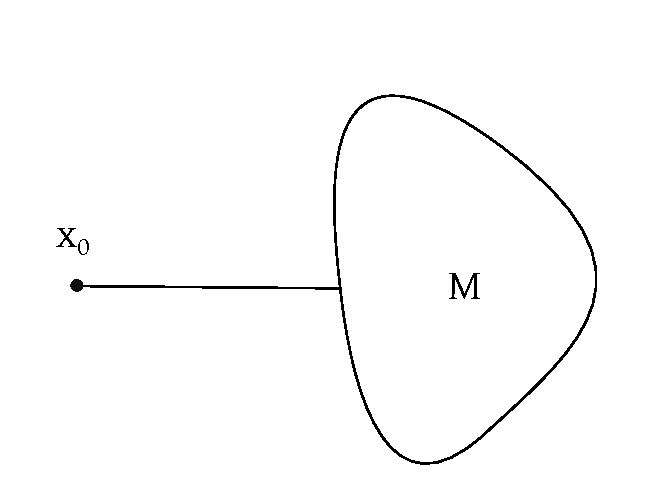
\includegraphics{img/08_generic_optimization_problem.pdf}
    \caption{A generic optimization problem}
    \label{optprob}
  \end{center}
\end{figure}

Now if $M$ is convex (consider $M$ convex in $(\mathbb R^n, \norm{\cdot}_2)$),
there exists a unique element $y \in M$ such that $\norm{x_0 - y}$ is minimal.

Finite elements (in computational mathematics) is the same idea.

\begin{theorem} % Satz 8.46
  $(V, \ip{\cdot}{\cdot})$ is a vector space with scalar product.
  $K \subseteq V$ is convex. Let $x \in V$ be given. Let $y_0 \in K$.
  Then the following statements are equivalent:
  \begin{enumerate}
    \item $\forall y \in K: \norm{x - y_0} \leq \norm{x - y}$
    \item $\forall y \in K: \Re\ip{x - y_0}{y - y_0} \leq 0$
    \item $\forall y \in K \setminus \set{y_0}: \norm{x - y_0} < \norm{x - y}$
  \end{enumerate}
  Compare with Figure~\ref{optconv}.
  In the special case if $K = U$ is a subspace, then the following statement is given (equivalent to statement~2)
  \begin{enumerate}
    \item[2'.] $\forall y \in U: \ip{x - y_0}{y - y_0} = 0$
  \end{enumerate}
\end{theorem}
\begin{figure}[!ht]
  \begin{center}
    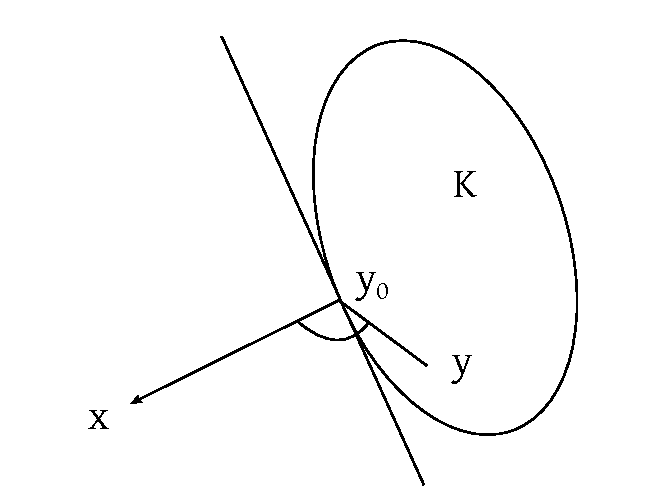
\includegraphics{img/09_optimization_on_a_convex_set.pdf}
    \caption{Optimization on a convex set}
    \label{optconv}
  \end{center}
\end{figure}

\begin{proof} \hfill{}
  \begin{enumerate}
    \item[1 $\to$ 2.]
      Let $y \in K: 1 > \varepsilon > 0$.
      \[ y_\varepsilon = \underbrace{y_0 + \varepsilon(y - y_0)}_{\varepsilon y + (1 - \varepsilon) y_0 \text{ because of convexity}} \in K \]
      \begin{align*}
        \forall \varepsilon \in (0,1): \norm{x - y_0}^2
          &\leq \norm{x - y_{\varepsilon}}^2 \\
          &= \norm{x - (y_0 + \varepsilon (y - y_0))}^2 \\
          &= \norm{(x - y_0) - \varepsilon(y - y_0)}^2 \\
          &= \norm{x - y_0}^2 - 2\varepsilon\Re\ip{x - y_0}{y - y_0} + \varepsilon^2 \norm{y - y_0}^2 \\
       \implies \forall 0 < \varepsilon < 1: 0
          &\leq -2\varepsilon \Re\ip{x - y_0}{y - y_0} + \varepsilon^2 \norm{y - y_0}^2 \\
          &= \varepsilon \cdot \left(- 2\Re\ip{x - y_0}{y - y_0} + \varepsilon \norm{y - y_0}^2\right) \\
          &\underbrace{\implies}_{\varepsilon \to 0} 0 \leq - 2\Re\ip{x - y_0}{y - y_0}
      \end{align*}
    \item[2 $\to$ 3.]
      \begin{align*}
        \norm{x - y}^2 &= \norm{(x - y_0) + (y_0 - y)}^2 \\
          &= \norm{(x - y_0) - (y - y_0)}^2 \\
          &= \norm{x - y_0}^2 + \norm{y - y_0}^2 \underbrace{- 2\Re\ip{x - y_0}{y - y_0}}_{\geq 0} \\
          &\geq \norm{x - y_0}^2 + \norm{y - y_0}^2 \\
          &> \norm{x - y_0}^2 \\
          & y \neq y_0
      \end{align*}
    \item[3 $\to$ 1.]
      trivial.
    \item[2 $\to$ 2'.]
      Consider $K = U$ is subspace.
      \[ \forall y \in Y: \Re\ip{x - y_0}{y - y_0} \leq 0 \]
      $U$ is a subspace.
      \[ \setdef{y - y_0}{y \in U} = \setdef{z}{z \in U} = U - y_0 \]

      \[
        \left.
        \begin{array}{ll}
          \forall z \in U: &\Re\ip{x - y_0}{z} \leq 0 \\
          \forall z \in U: &\Re\ip{x - y_0}{-z} \leq 0
        \end{array}
        \right\}
        \implies \forall z \in U: \Re\ip{x - y_0}{z} = 0
      \]
      Case $K = \mathbb C$:
      \[ i \cdot U = U \]
      \[ \implies z \in U: \Re\ip{x - y_0}{iz} = 0 \]
      \[ \Re\overline{i}\ip{x - y_0}{z} = \Im\ip{x - y_0}{z} \]
  \end{enumerate}
\end{proof}

\begin{corollary}
  Let $(V, \angel{\cdot,\cdot})$ be a vector space.
  \begin{enumerate}
    \item $K \subseteq V$ is convex, $x \in V$.
      Then the optimization problem
      \[
        \left\{\begin{array}{c}
          \norm{x - y} = \min! \\
          y \in K
        \end{array}\right.
      \]
      has at most one solution.
    \item If $K = U$ subspace,
      then there exists at most one $y_0 \in U$ such that $x - y_0 \in U^\bot$.
  \end{enumerate}
\end{corollary}

\dateref{2018/04/23}

Orthonormal basis:
\[ \ip{b_i}{b_j} = \delta_{ij} \]
\[ v = \sum \lambda_i b_i \leadsto \ip{v}{b_i} = \lambda_i \]
Given: an arbitrary basis of a subspace \\
Find: orthonormal basis of the subspace

\begin{figure}[t]
  \begin{center}
    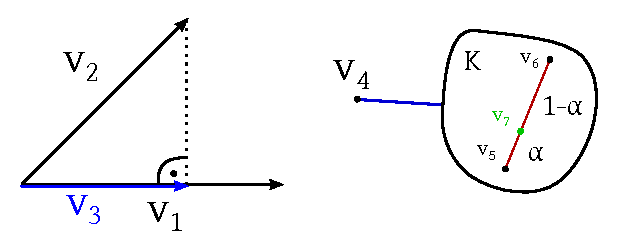
\includegraphics{img/09b_projection_and_convexity.pdf}
    \caption{
      Projection of vector $v_1$ onto vector $v_2$ results in projected vector $v_3$ (left).
      $K$ is a convex set (right). Due to convexity, there is a unique shortest path of $v_4$ to $K$.
      And a convex set satisfies for any two $v_5, v_6 \in K$ that $v_7 \in K$ with $v_7 = (v_6 - v_5) \lambda$ where $\lambda \in [0, 1]$
    }
  \end{center}
\end{figure}

\[ K \subseteq V \text{ convex} \]
$V$ with scalar product.

Then the optimization problem
\[ \norm{x - y} = \min \qquad Y \in K \]
has at most one solution.

$y$ is the solution.
\[ \iff \Re\ip{x-y_0}{y - y_0} \leq 0 \forall y \in K \]
If $K$ is the subspace $U$ ($x - y_0 \bot U$), then
\[ \Re\ip{x - y_0}{y} = 0 \forall y \in K \]

\[ U^\bot = \setdef{y}{y \bot U} \]
is subspace.
\[ U \cap U^\bot = \set{0} \]
If $x \in U \cap U^\bot$, then $x \bot x = \ip{x}{x} = \norm{x}^2 = 0$.

Orthogonal complement: $U + U^\bot$ is direct sum. \\
Every $x \in U + U^\bot$ has a unique decomposition.
\[ x = u + v \qquad u \in U, v \in U^\bot \]
The maps $x \mapsto u$ and $x \mapsto v$ are linear.

\begin{definition}
  Assume $U \dot+ U^\bot = V$.
  Then the projection maps
  \[ \pi_U: V \to V \qquad \pi_U^\bot: V \to V \]
  such that $\pi_U(x) \in U$ and $\pi_{U^\bot}(x) \in U^\bot$ and $x = \pi_U(x) + \pi_{U^\bot}(x)$ are orthogonal projections.
\end{definition}

\begin{Remark}
  \begin{enumerate}
    \item $x \in U \iff \pi_U(x) = x \iff \pi_{U^\bot}(x) = 0$
    \item $x \in U^\bot \iff \pi_U(x) = 0 \iff \pi_{U^\bot}(x) = x$
    \item $\pi_{U^\bot} = \operatorname{id} - \pi_U$
  \end{enumerate}
\end{Remark}

\[ \pi_U(x) \in U \]
\[ \implies \text{remark (4): } \pi_U(\pi_U(x)) = \pi_U(x) \]
\[ \text{($\sim$): } \pi_U \circ \pi_U = \pi_U \text{ idempotent} \]
\[ \pi_U \text{ is linear: } \pi_U \circ \pi_{U^\bot} = 0 \]

\begin{theorem} % 8.50
  Let $V = U \dot+ U^{\bot}$.
  \begin{enumerate}
    \item $\forall x, y \in V: \ip{x}{\pi_{U}(y)} = \ip{\pi_U(x)}{y} = \ip{\pi_U(x)}{\pi_U(y)}$
    \item Compare with Figure~\ref{img:proj}.
        \[ \norm{\pi_U(x)} \leq \norm{x} \land \norm{\pi_U(x)} = \norm{x} \iff x \in U \]
        Proof:
        \begin{enumerate}
          \item
            \[ x = \pi_U(x) + \pi_{U^\bot}(x) \qquad y = \pi_U(y) + \pi_{U^\bot}(y) \]
            \[ \ip{x}{\pi_U(y)} = \ip{\pi_U(x) + \pi_{U^\bot}(x)}{\pi_U(y)} = \ip{\pi_U(x)}{\pi_U(y)} + \underbrace{\ip{\underbrace{\pi_U(x)}_{\in U^\bot}}{\underbrace{\pi_U(y)}_{\in U}}}_{= 0} \]
            \[ \ip{\pi_U(x)}{y} = \ip{\pi_U(x)}{\pi_U(y)} + \ip{\pi_U(x)}{\pi_{U^\bot}(y)} \]
          \item
            \[ x = \pi_U(x) + \pi_{U^\bot}(x) \]
            \[ \implies \norm{x}^2 = \norm{\pi_U(x)}^2 + \norm{\pi_{U^\bot}(x)}^2 \geq \norm{\pi_U(x)}^2 \]
            By equality $\iff \norm{\pi_{U^\bot}(x)} = 0 \iff x = \pi_U(x) \iff x \in U$
        \end{enumerate}
        \begin{figure}[!ht]
          \begin{center}
            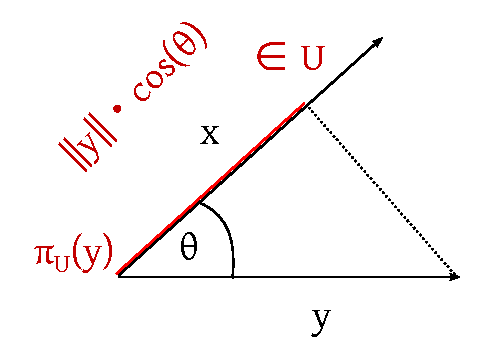
\includegraphics{img/10_projection.pdf}
            \caption{Projection}
            \label{img:proj}
          \end{center}
        \end{figure}
  \end{enumerate}
\end{theorem}

\begin{Person}
  J{\o}rgen Pedison Gram (1850--1916)
\end{Person}

\index{Gram matrix of tuple $v_1, v_2, \ldots, v_m$}
\begin{definition} % 8.51
  Let $v_1, v_2, \ldots \in V$.
  \[
    \operatorname{Gram}(v_1, \ldots, v_m) = \begin{bmatrix}
      \ip{v_1}{v_1} & \ip{v_1}{v_2} & \ldots & \ip{v_1}{v_m} \\ 
      \ip{v_2}{v_1} & \ip{v_2}{v_2} & \ldots & \ip{v_2}{v_m} \\ 
      \vdots & \vdots & \vdots & \vdots \\
      \ip{v_m}{v_1} & \ip{v_m}{v_2} & \ldots & \ip{v_m}{v_m}
    \end{bmatrix}
  \]
  is called \emph{Gram matrix of tuple $v_1, v_2, \ldots, v_m$}
\end{definition}

\begin{remark} % Bemerkung 8.52
  In case $V = \mathbb C^n$.
  \[ \ip vw = \overline{w}^T \cdot v = \sum_{i=1}^n \lambda_i \overline{\mu_i} = (\overline \mu_1, \ldots, \overline \mu_n)\begin{pmatrix} \lambda_1 \\ \vdots \\ \lambda_n \end{pmatrix} \]
  \[ v = \begin{pmatrix} \lambda_1 \\ \vdots \\ \lambda_n \end{pmatrix} \qquad w = \begin{pmatrix} \mu_1 \\ \vdots \\ \mu_n \end{pmatrix} \]
  Hence, if
  \[ v_i = \begin{pmatrix} \beta_{1i} \\ \vdots \\ \beta_{ni} \end{pmatrix} \qquad i = 1, \ldots, m \]

  \begin{align*}
    V &= \begin{pmatrix} v_1 & v_2 & \ldots & v_m \\ \vdots & \vdots & & \vdots \end{pmatrix} \in \mathbb C^{n \times m} \\
      &= \begin{pmatrix} \beta_{11} & \beta_{12} & \ldots & \beta_{1m} \\ \vdots & \vdots & & \vdots \\ \beta_{n1} & \beta_{n2} & \ldots & \beta_{nm} \end{pmatrix} \\
    (V^*V)_{ij} &= \sum_{k=1}^n (v^*)_{ik} v_{kj} = \sum_{k=1}^n \overline{\beta_{ki}} \beta_{kj} = \overline{\ip{v_i}{v_j}} \\
      &= \begin{pmatrix} v_1^* & \ldots \\ \vdots & \\ v_m^* & \ldots \end{pmatrix} \begin{pmatrix} v_1 & \ldots & v_m \\ \vdots &  & \vdots \end{pmatrix}
  \end{align*}
  \[ V^* V = \overline{\operatorname{Gram}(v_1, \ldots, v_m)} \]
\end{remark}

\begin{theorem} % 8.23
  Let $v_1, \ldots, v_m \in V$. $G = \operatorname{Gram}(v_1, \ldots, v_m)$.
  \begin{enumerate}
    \item $G = G^*$ is Hermitian, positive \emph{semi}definite.
      \[ \xi^T \cdot G \cdot \overline{\xi} = \norm{\sum_{i=1}^m \xi_i v_i}^2 \geq 0 \]
    \item $\xi \in \ker{G} \iff \sum_{i=1}^m \overline{\xi_i} v_i = 0$
    \item $G$ is positive definite iff $(v_1, \ldots, v_m)$ are linear independent.
  \end{enumerate}
\end{theorem}

\begin{proof}
  \begin{enumerate}
    \item $g_{ij} = \ip{v_i}{v_j} = \overline{\ip{v_j}{v_i}} = \overline{g_{ji}}$
      \[ \xi^T \cdot G \cdot \overline{\xi} = \sum_{i=1}^n \sum_{j=1}^n \xi_i g_{ij} \overline{\xi_j} = \sum_{i=1}^n \sum_{j=1}^n \xi_i \overline{\xi_j} \ip{v_i}{v_j} = \ip{\sum_{i=1}^n \xi_i v_i}{\sum_{j=1}^n \xi_j v_j} = \norm{\sum_{i=1}^n \xi_i v_i}^2 \]
    \item
      Direction $\implies$.
      $\xi \in \ker{G} \implies G \xi = 0 \implies \xi^T \cdot G \cdot \xi = 0$
      \[ \xi^T \cdot G \cdot \xi = \xi^T \cdot G \cdot \overline{\overline{\xi}} \underbrace{=}_{(1)} \norm{\sum_{i=1}^m \overline{\xi_i} v_i}^2 \]
      Direction $\impliedby$. If $\norm{\sum_1^m \xi_i v_i} = 0$
      \[ (G \cdot \xi)_i = \sum_{j=1}^n \ip{v_i}{v_j} \xi_j = \sum_{j=1}^n \ip{v_i}{\overline{\xi_j} v_j} = \ip{v_i}{\underbrace{\sum_{j=1}^n \overline{\xi_j}}_{=0} v_j} = 0 \]
      \[ \implies G \cdot \xi = 0 \]
    \item $G$ is positive definite
      \begin{align*}
        &\iff \forall \xi \neq 0: \xi^T \cdot G \cdot \overline \xi > 0 \\
        &\iff \forall \xi \neq 0: \norm{\sum_1^m \xi_i \cdot v_i}^2 > 0 \\
        &\iff \forall \xi \neq 0: \sum_{i=1}^m \xi_i v_i \neq 0 \\
        &\iff (v_1, \ldots, v_m) \text{ is linear independent} \\
        &\iff \ker{G} = \set{0} \\
        &\iff G \text{ is invertible}
      \end{align*}
  \end{enumerate}
\end{proof}

\begin{theorem} % 8.54
  Let $U \subseteq V$ be a subspace. $V$ is a vector space with scalar product.
  \[ (u_1, \ldots, u_m) \text{ is basis of } U \qquad
     G = \operatorname{Gram}(u_1, \ldots, u_m) = \left[\ip{u_i}{u_j}\right]_{i,j=1,\ldots,m} \]
  Then the projection is $\pi_U(x) = \sum_{j=1}^m \eta_j u_j$ where
  $ \eta = \overline{G}^{-1} \cdot \begin{pmatrix} \ip{x}{u_1} & \dots & \ip{x}{u_m} \end{pmatrix}^T $.
  Additionally, if $u_1, \ldots, u_m$ would be an orthonormal basis, then the coordinate of $x$ is given by
  $ \begin{pmatrix} \ip{x}{u_1} & \dots & \ip{x}{u_m} \end{pmatrix}^T $.
\end{theorem}

\begin{figure}[t]
  \begin{center}
    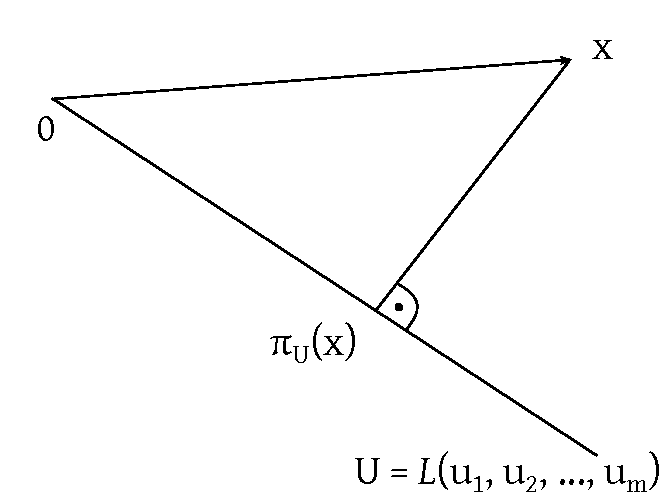
\includegraphics{img/11_projection.pdf}
    \caption{Projection $\pi_U(x)$ of $x$ onto $U$}
    \label{img:projection}
  \end{center}
\end{figure}

\begin{proof}
  Let $u = \sum_{j=1}^m \eta_j u_j$. Compare with Figure~\ref{img:projection}.
  Show that $x - u \in U^{\bot} = \mathcal L(u_1, \ldots, u_m)^\bot = \set{u_1, \ldots, u_m}^\bot = \bigcap_{i=1}^m u_i^\bot$.
  Hence, show that $x - u \bot u_i \forall i \in \set{1, \ldots, m}$.

  \begin{align*}
    \ip{u_i}{u} &= \ip{u_i}{\sum_{j=1}^m \eta_j u_j}
      = \sum_{j=1}^m \ip{u_i}{u_j} \cdot \overline{\eta_j}
      = \sum_{j=1}^m g_{ij} \overline{\eta_j} \\
      &= (G \overline{\eta})_i
      = \ip{u_i}{x}
  \end{align*}
  because
  \[
    \overline G \cdot \eta = \begin{pmatrix} \ip{x}{u_1} \\ \vdots \\ \ip{x}{u_m} \end{pmatrix}  \qquad
    G \cdot \overline \eta = \begin{pmatrix}
      \overline{\ip{x}{u_1}} \\
      \vdots \\
      \overline{\ip{x}{u_m}}
    \end{pmatrix} =
    \begin{pmatrix}
      \ip{u_1}{x} \\
      \vdots \\ 
      \ip{u_m}{x}
    \end{pmatrix}
  \]
  Hence, $\forall i \in \set{1, \ldots, m}$:
  \[ \ip{u_i}{u} = \ip{u_i}{x} \implies \forall i \in \set{1, \ldots, m}: \ip{u_i}{x - u} = 0 \implies x - u \in \set{u_1, \ldots, u_m}^\bot \]
\end{proof}

\begin{example} % Beispiel 8.55
  \label{ex855}
  Find polynomial $p(t)$ of degree $2$ such that
  \[ \int_0^1 \card{t^3 - p(t)}^2 \, dt \overset!= \min \]
  $V = C[0,1]$, scalar product
  \[ \ip{f}{g} = \int_0^1 f(t) \overline{g(t)} \, dt \]
  \begin{align*}
    U &= \text{ polynomial function of degree } \leq 2 \\
    x &= t \mapsto t^3 \not\in U
  \end{align*}
  Find $p \in U$ such that $\norm{x - p}^2 \overset!= \min$
  \[ \norm{x - p}^2 = \int \card{x(t) - p(t)}^2 \, dt \]
  Basis of $U = \mathcal L(\set{1, t, t^2})$
  \[ u_i(t) = t^{i-1} \qquad i = 1,2,3 \]
  Gram matrix:
  \[ g_{ij} = \ip{u_i}{u_j} = \int_0^1 t^{i-1} t^{j-1} \, dt = \int_0^1 t^{i+j-2} \, dt = \left. \frac{t^{i+j-1}}{i + j - 1} \right|_0^1 = \frac{1}{i + j - 1} \]
  \[
    G = \begin{bmatrix}
      1 & \frac12 & \frac13 \\
      \frac12 & \frac13 & \frac14 \\
      \frac13 & \frac14 & \frac15
    \end{bmatrix}
  \]
  Hilbert matrix:
  \[ \left[\frac{1}{i+j-1}\right]_{i,j=1,\ldots,k} \]
  This matrix is very unstable (in the equation system $Gx = b$) and therefore a very important test matrix in computational mathematics (ie. Numerics).

  \[ u = \sum_{j=1}^3 \eta_j u_j \qquad \eta = \overline{G}^{-1} \cdot \begin{pmatrix} \ip{x}{u_1} \\ \ip{x}{u_2} \\ \ip{x}{u_3} \end{pmatrix} \]
  \[ \ip{x}{u_j} = \int_0^1 x(t) u_j(t) \, dt = \int_0^1 t^3 \cdot t^{j-1} \, dt = \int_0^1 t^{2 + j} \, dt = \frac{1}{3 + j} \]
  \[
    \eta = \begin{bmatrix} 1 & \frac12 & \frac13 \\ \frac12 & \frac13 & \frac14 \\ \frac13 & \frac14 & \frac15 \end{bmatrix}^{-1}
    \begin{pmatrix} \frac14 \\ \frac15 \\ \frac16 \end{pmatrix}
    = \begin{bmatrix} 9 & -36 & 30 \\ -36 & 192 & -180 & 30 & -180 & 180 \end{bmatrix}
    \begin{bmatrix} \frac14 \\ \frac15 \\ \frac16 \end{bmatrix}
    = \begin{bmatrix} \frac1{20} \\ -\frac35 \\ \frac32 \end{bmatrix}
  \]
  (Assume that we don't know $180$ in the bottom-right corner precisely. Consider $180+\varepsilon$, then this error $\varepsilon$ explodes tremendously in the solution).
\end{example}

\begin{corollary} % 8.56
  \label{ONRcor}
  Special case $u_i$ is orthonormal basis of $U$ ($\rightarrow G = I$)
  Then it holds that
  \begin{enumerate}
    \item $\forall v \in V: \pi_U(v) = \sum_{i=1}^m \ip{v}{v_i} \cdot u_i$
    \item
      \[ \norm{v}^2 \geq \sum_{i=1}^m \card{\ip{v}{v_i}}^2 \qquad \text{ (Bessel's inequality)} \]
      \[ \norm{v}^2 = \sum_{i=1}^m \card{\ip{v}{u_i}}^2 \iff v \in U \qquad \text{ (Parseval's identity)} \]
      \[ \eta_j = \overline{G}^{-1}\begin{pmatrix} \ip{v}{u_1} \\ \vdots \\ \ip{v}{u_m} \end{pmatrix} \]
  \end{enumerate}
\end{corollary}

\begin{Person}
  Friedrich Bessel (1784--1846)
\end{Person}
\begin{Person}
  Marc-Antoine Parseval (1755--1836)
\end{Person}

\begin{proof}
  Gram's matrix = $I$.
  \[ \eta_j = \ip{v}{u_j} \]
\end{proof}

\subsection{Gram-Schmidt process}

\textbf{Given:} finite, linear independent vectors $v_1, \dots, v_m$ \\
\textbf{Find:} orthonormal basis of $(v_1, \dots, v_m)$.

\index{Gram-Schmidt process}
\begin{theorem}[Gram–Schmidt process for orthogonalization] % 8.57
  Let $(v_1, \ldots, v_m) \subseteq V$ be linear independent.
  Let $U \coloneqq \mathcal L(v_1, \ldots, v_m)$.
  Then $\exists u_1, \ldots, u_m$ as orthonormal basis of $U$, specifically inductive
  \[ u_1 = \frac{v_1}{\norm{v_1}} \]
  and for $k = 2, \ldots, m$:
  \[ \tilde u_k = v_k - \sum_{j=1}^{k-1} \ip{v_k}{u_j} \cdot u_j \qquad
     u_k = \frac{\tilde{u_k}}{\norm{u_k}} \]
  \begin{figure}[t]
    \begin{center}
      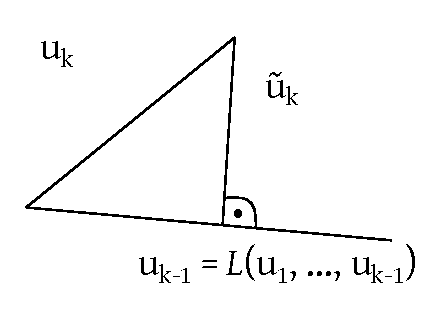
\includegraphics{img/12_GS_projection.pdf}
      \caption{Projection used in the Gram-Schmidt process}
      \label{GSproj}
    \end{center}
  \end{figure}
\end{theorem}

\begin{proof}
  \begin{description}
    \item[Induction base] $k=1$ is trivial
    \item[Induction step] $k-1 \to k$. Assume
      \[ \mathcal L(u_1, \ldots, u_{k-1}) = \mathcal L(v_1, \ldots, v_{k-1}) \eqqcolon U_{k-1} \]
      \[ \tilde u_k = v_k - \pi_{U_{k-1}}(v_k) \in U_{k-1}^\bot \text{ because of Theorem~\ref{ONRcor}} \]
      \[ \implies \tilde u_k \bot u_1, \ldots, u_{k-1} \implies (u_1, \ldots, u_{k-1}, \frac{\tilde u_k}{\norm{\tilde u_k}}) \]
      is an orthonormal basis.
      \[
        \mathcal L(u_1, \ldots, u_{n-1}, \frac{\tilde u_k}{\norm{\tilde u_k}})
          = \mathcal L(u_1, \ldots, u_{k-1}, v_k)
      \]
      then $\tilde u_k - v_k \in \mathcal L(u_1, \ldots, u_{k-1})$
  \end{description}
\end{proof}

\dateref{2018/04/25}

Gram-Schmidt process:
\[ \mathcal L(v_1, v_2) = \mathcal L(v_2 - p(v_2), v_1) \qquad v_2 - p(v_2) \bot v_1 \]

Given: $v_1, \ldots, v_m$
\[ u_i = \frac{v_i}{\norm{v_i}} \]
\[ \tilde u_k = v_k - \sum_{i=1}^{k-1} \ip{v_k}{u_i} \cdot u_i \]
\[ u_k = \frac{\tilde u_k}{\norm{\tilde u_k}} \qquad \frac{\ip{v_k}{\tilde u_i} \tilde u_i}{\norm{\tilde u_i}^2} \]

\begin{Example}
  Let $V = \mathbb R^3$.
  \[ \ip xy = x^t A y \]
  \[
    A = \begin{bmatrix}
      1 & -1 & 1 \\
      -1 & 3 & -1 \\
      1 & -1 & 2
    \end{bmatrix}
  \]
  \[ v_i = \text{ standard basis } e_i \]
  \[ \norm{v_1}^2 = \ip{v_1}{v_1} = v_1^T A v_1 = a_{11} = 1 \]
  \[ \norm{v_2}^2 = \ip{v_2}{v_2} = a_{12} = 3 \]
  \[ u_1 = \frac{v_1}{\norm{v_1}} = \begin{pmatrix} 1 \\ 0 \\ 0 \end{pmatrix} \]
  \[ \tilde u_2 = v_2 - u_1 \ip{v_2}{u_1} = \begin{pmatrix} 0 \\ 1 \\ 0 \end{pmatrix} - \begin{pmatrix} 1 \\ 0 \\ 0 \end{pmatrix} \cdot (0 \: 1 \: 0) A \begin{pmatrix} 1 \\ 0 \\ 0 \end{pmatrix} = \begin{pmatrix} 0 \\ 1 \\ 0 \end{pmatrix} + \begin{pmatrix} 1 \\ 0 \\ 0 \end{pmatrix} = \begin{pmatrix} 1 \\ 1 \\ 0 \end{pmatrix} \]
  \[ u_2 = \frac{\tilde u_2}{\norm{\tilde u_2}} \qquad \norm{\tilde u_2}^2 = \ip{\tilde u_2}{\tilde u_2} = (1 \: 1 \: 0) \cdot A \begin{pmatrix} 1 \\ 1 \\ 0 \end{pmatrix} = 2 \qquad u_2 = \frac{1}{\sqrt2} \begin{pmatrix} 1 \\ 1 \\ 0 \end{pmatrix} \]
  \[ \tilde u_3 = v_3 - u_1 \ip{v_3}{u_1} - u_2 \ip{v_3}{u_2} \]
  \[ = \begin{pmatrix} 0 \\ 0 \\ 1 \end{pmatrix} - \vecthree100 \cdot \underbrace{(0 \: 0 \: 1) \cdot A \cdot \vecthree100}_{a_{31} = 1} - \frac{1}{\sqrt{2}} \vecthree110 \cdot \underbrace{(0 \: 0 \: 1) \cdot A \cdot \vecthree110}_{a_{31} + a_{32} = 0} \cdot \frac{1}{\sqrt2} = \vecthree{-1}01 \]
  \[ \norm{\tilde u_3}^2 = (-1 \: 0 \: 1) \cdot A \cdot \vecthree{-1}{0}1 = 1 - 1 - 1 + 2 = 1 \qquad u_3 = \vecthree{-1}{0}{1} \]
\end{Example}

\begin{remark} % 8.59
  This is an alternative method to build orthogonal projection on subspace $U \subseteq \mathbb C^n$ with standard scalar product.
  \begin{enumerate}
    \item Determine an orthonormal basis of $U$: $u_1, \ldots, u_m \in \mathbb C^{n\times 1}$
    \item $P = \sum_{i=1}^m u_1 \cdot u_i^*$
  \end{enumerate}
  \[ P \cdot v = \sum_{i=1}^m u_i \underbrace{u_i^* \cdot v}_{\ip{v}{v_i}} = \sum_{i=1}^m u_i \ip{v}{v_i} \]
  Gram matrix = $I$
\end{remark}

\begin{example}[Example~\ref{ex855} again] % 8.60
  \[ V = C[0,1] \qquad U = \mathcal L(1, x, x^2) \eqqcolon \mathcal L(v_1, v_2, v_3) \]
  \[ \ip fg = \int_0^1 f(t) \overline{g(t)} \, dt \]
  Orthonormal basis:
  \[ \norm{v_i}^2 = \int_0^1 1^2 \, dt = 1 \]
  \[ u_1 = 1 \]
  \[ \tilde u_2 = v_2 - u_1 \cdot \ip{v_2}{u_1} = x - 1 \cdot \underbrace{\int_0^1 t \cdot 1 \, dt}_{= \frac12} = x - \frac12 \]
  \[ \norm{\tilde u_2}^2 = \int_0^1 (t - \frac12)^2 \, dt = \left.\frac{(t - \frac12)^3}{3} \right|_0^1 = \frac{(\frac12)^3 - (-\frac12)^2}{3} = \frac1{12} \]
  \[ u_2 = \frac{\tilde u_2}{\norm{\tilde u_2}} = \sqrt{12} \cdot (x - \frac12) \]
  \begin{align*}
    \tilde u_3 &= v_3 - u_1 \ip{v_3}{u_1} - u_2 \cdot \ip{v_3}{u_2} \\
      &= x^2 - 1 \cdot \underbrace{\int_0^1 t^2 \cdot 1 \, dt}_{= \frac13} - \sqrt{12} (x - \frac12) \int_0^1 t^2 \sqrt{12} (t - \frac12) \, dt \\
      &= x^2 - \frac13 - 12 (x - \frac12) \cdot \frac1{12} \\
      &= x^2 - x + \frac16
  \end{align*}
  Side note:
  \[ \int_0^1 t^2 (t - \frac12) \, dt = \int_0^1 (t^3 - \frac12 t^2) \, dt = \frac14 - \frac16 = \frac1{12} \]
  \[ \norm{\tilde u_3}^2 = \int_0^1 (t^2 - t + \frac16)^2 \, dt = \frac1{180} \]
  \[ \implies u_3 = \sqrt{180} \cdot (x^2 - x + \frac16) \]

  Projection:
  \[ \int_0^1 (t^3 - p(t))^2 \, dt = \operatorname{min}! \]
  Solution: $\pi_U(x^3) \qquad U = \mathcal L(1, x, x^2)$
  \begin{align*}
    \pi_U(x^3) &= u_1 \ip{x^3}{u_1} + u_2 \ip{x^3}{u_2} + u_3 \ip{x^3}{u_3} \\
      &= 1 \cdot \int_0^1  t^3 \cdot 1 \, dt + \sqrt{12} \left(x - \frac12\right) \int_0^1 t^3 \sqrt{12} \left(t - \frac12\right) \, dt \\
      &+ \sqrt{180} \left(x^2 - x + \frac16\right) \int_0^1 t^3 \sqrt{180} \left(t^2 - t + \frac16\right) \, dt
  \end{align*}
\end{example}

\index{Chebyshev polynomials}
Consider $\ip fg \coloneqq \int_{-1}^1 \sqrt{1 - t^2} f(t) \overline{g(t)} \, dt$.
Take $1, x, x^2, \ldots$ and apply Gram-Schmidt process to retrieve the Chebyshev polynomials.
\begin{align*}
  \int_0^1 f(t) g(t) \, dt &\qquad \text{ Laguerre polynomials} \\
  \frac1{\sqrt{2\pi}} \int_{-\infty}^\infty e^{-\frac{t^2}{2}}  f(t) g(t) \, dt &\qquad \text{ Hermite polynomials}
\end{align*}

\subsection{Riesz representation theorem}

\begin{Person}
  Frigyes Riesz (1880--1956)
\end{Person}

\begin{theorem} % 8.61
  Let $(V, \ip{\cdot}{\cdot})$ be a vector space with scalar product $\dim{V} < \infty$.

  $V^*$ is the dual space, namely $\operatorname{Hom}(V, \mathbb K)$ which is the space of linear functionals.
  For some fixed $y \in V$, the map $T_y(x) = \ip{x}{y}$ is linear in $x$ (and therefore $T_y \in V^*$).

  Then the map $V \to V^*$ (where an element of $V^*$ is a map $V \to \mathbb K$ with $x \mapsto \ip xy$)
  is an antilinear isomorphism (antiisomorphism).
\end{theorem}

This is trivial in $\mathbb R$, but in $\mathbb C$ it is much more complex (pun intended).

Hence,
\begin{enumerate}
  \item For every $y$ it holds that $Ty \in V^*$
  \item For every linear functional $f \in V^*: \exists! y \in V: f = T_y$
  \item Let $y \mapsto Ty$ be an antilinear map.
    \[ T_{\lambda y_1 + \mu y_2} = \overline{\lambda} Ty_1 + \overline{\mu} Ty_2 \]
\end{enumerate}

\begin{Example}[For point 2]
  \[ V = C[0,1] \]
  Scalar product: $\ip fg = \int f(t) g(t) \, dt$.
  Let $F: C[0,1] \to \mathbb R$ linear.
  Then by the Riesz representation theorem,
  there exists $g \in C[0,1]: F(f) = \int f(t) g(t) \, dt$.

  For example $f \to f(1)$
  \[ \exists g(t): f(1) = \int_0^1 f(t) g(t) \, dt \]
  In physics, e.g. the Dirac delta function.
\end{Example}

\begin{proof}[Proof of point 3]
  We show linearity.

  \[ Ty(x) = \ip xy \text{ is linear in } X \implies T_y \in V^* \]
  \begin{align*}
    \forall x \in V: T_{\lambda y_1 + \mu y_2}(x)
      &= \ip{x}{\lambda y_1 + \mu y_2} = \overline{\lambda} \ip{x}{y_1} + \overline{\mu}\ip{x}{y_2} \\
      &= \overline{\lambda} Ty_1(x) + \overline{\mu} Ty_2(x) = (\overline{\lambda} Ty_1 + \overline{\mu} Ty_2)(x) \\
      &\implies T_{\lambda y_1 + \mu y_2} = \overline{\lambda} Ty_1 + \overline{\mu} Ty_2
  \end{align*}
  
  We show injectivity: the map $y \mapsto Ty$ is injective.

  Assume: $Ty = 0$ (zero functional). Show $y = 0$.
  $Ty = 0$ means $\forall x \in V: Ty(x) = 0$, especially for $x = y$, $T_y(y) = \ip yy = 0 \implies y = 0$.

  We show surjectivity: the map $y \mapsto Ty$ is surjective.

  Let $u_1, \ldots, u_n$ be an orthonormal basis (exists because of Gram-Schmidt).
  
  Given: $f \in V^*$.
  Find: $y$ such that $f = Ty$.
  \[ \text{Hence, } \forall x \in V: f(x) = \ip xy \underbrace{\iff}_{\text{by \foreignlanguage{german}{Fortsetzungssatz}}} f(u_i) = \ip{u_i}{y} \]
  Let $y = \sum_{j=1}^n \overline{f(u_j)} \cdot u_j$.
  \[ \implies \ip{u_i}{y} = \ip{u_1}{\sum_{j=1}^n \overline{f(u_j)} u_j} = \sum_{j=1}^n f(u_j) \underbrace{\ip{u_i}{u_j}}_{\delta_{ij}} = f(u_i) \]
  Hence, $y$ satisfies the condition.
\end{proof}

\begin{Remark}
  The Riesz representation theorem also holds in infinite dimensions (thus, in Hilbert spaces, a generalization of Euclidean spaces).
  In those spaces, there exists some Hilbert base:
  \[ (u_i)_{i \in I}: x = \sum_{i \in I} \ip x{u_i} \cdot u_i \forall x \]
  So every $x$ has such a representation and in infinite dimensions, this representation is a series.
\end{Remark}

\begin{corollary}\hfill{} % Folgerungen 8.62
  \begin{enumerate}
    \item $v = 0 \iff \forall w \in V: \ip vw = 0$
    \item $\norm{v} = \sup\setdef{\card{\ip vw}}{\norm{w} \leq 1}$
  \end{enumerate}
  Equivalently in the dual space:
  \begin{enumerate}
    \item $v = 0 \iff \forall f \in V^*: f(v) = 0$
    \item $\norm{v} = \sup\setdef{\card{f(v)}}{f \in V^*, \norm{f} \leq 1}$
  \end{enumerate}
  holds in general in a normed space.
\end{corollary}

\begin{Remark}
  We make a small revision: dual space $V^* = \operatorname{Hom}(V, \mathbb K)$
  \[ W \xrightarrow{T} V \xrightarrow{f} \mathbb K \]
  \[ \implies f \circ T: W \to \mathbb K \in W^* \]
  is a linear functional on $W$.
  Hence, the map $\operatorname{Hom}(V, \mathbb K) \to \operatorname{Hom}(W, \mathbb K)$ and $f \mapsto f \cdot T$ is linear.
  \[ (\lambda f + \mu g) \circ T = \lambda \cdot f_0 T + \mu g \circ T \qquad \text{\enquote{transposed map}} \]
  Linear map: $T^*: V^* \to W^*$.

  Let $V$, $W$ be spaces with a scalar product. Then $V \simeq V^*$ and $W \simeq W^*$ where $\simeq$ means anti-isomorphic.
  $T: W \to V \implies T^*: V \to W$.
\end{Remark}

\subsection{Adjoint maps}
\index{Adjoint map}
\begin{definition}[Theorem and definition] % 8.63
  \label{def863}
  Let $(V, \ip{\cdot}{\cdot}_V)$ and $(W, \ip{\cdot}{\cdot}_W)$ be spaces with a scalar product. $\dim{V}, \dim{W} < \infty$.
  \[ T \in \operatorname{Hom}(W, V) \text{ hence, } T: W \to V \text{ linear} \]
  \begin{enumerate}
    \item For every $v \in V$ the map $w \mapsto \ip{T(w)}{v}_V$ is linear.
    \item $\forall v \in V \exists! u \in W \forall w \in W: \ip{T(w)}{v}_V = \ip{w}{u}_W$ and $T^*(v) = u$. \\
      Hence,
      \[ \ip{T(w)}{v}_V = \ip{w}{T^*(v)}_W \qquad \forall w \in W \quad \forall v \in V \]
    \item The map $T^*: V \to W$ with $v \mapsto u$ is linear, hence $T^* \in \operatorname{Hom}(V, W)$ and is called \emph{adjoint map}.
    \item The map $\operatorname{Hom}(W, V) \mapsto \operatorname{Hom}(V, W)$ with $T \mapsto T^*$ is antilinear and $T^{**} = T$.
  \end{enumerate}
\end{definition}

\begin{proof}
  \begin{enumerate}
    \item $\ip{T(w)}{v} = T_V(T(w)) = T_v \circ T(w)$ \\
      Composition of linear maps is linear.
    \item $T_V \circ T \in W^*$. By Riesz representation theorem, $\exists! u \in W: T_V \circ T(w) = \ip{w}{u} \forall w \in W \implies \ip{T(w)}{v} = \ip wu$
    \item Show that,
      \[ \forall v_1, v_2 \in V \forall \lambda, \mu: T^*(\lambda v_1 + \mu v_2) = \lambda T^*(v_1) + \mu T^*(v_2) \]
      It suffices to show that
      \[ \ip{w}{T^*(\lambda v_1 + \mu v_2)} = \ip{w}{\lambda T^*(v_1) + \mu T^*(v_2)} \forall w \in W \]
      Compare with corollary: $w_1 = w_2$ in $W \iff \forall w: \ip{w}{w_1} = \ip{w}{w_2}$.
      \begin{align*}
        \ip{w}{T^*(\lambda v_1 + \mu v_2)} &= \ip{T(w)}{\lambda v_1 + \mu v_2} \\
          &= \overline{\lambda} \ip{T(w)}{v_1} + \overline{\mu} \ip{T(w)}{v_2} \\
          &= \overline{\lambda} \ip{w}{T^*(v_1)} + \overline{\mu} \ip{w}{T^*(v_2)} \\
          &= \ip{w}{\lambda T^*(v_1)} + \ip{w}{\mu T^*(v_2)} \\
          &= \ip{w}{\lambda T^*(v_1) + \mu T^*(v_2)}
      \end{align*}
    \item Show $(\lambda T_1 + \mu T_2)^* = \overline{\lambda} T_1^* + \overline{\mu} T_2^*$. \\
      \[ \iff \forall v \in V: (\lambda T_1 + \mu T_2)^* v = (\overline{\lambda} T_1^* + \overline{\mu} T_2^*)(v) \]
      \[ \forall v \in V \forall w \in W: \ip{w}{(\lambda T_1 + \mu T_2)^*(v)} = \ip{w}{(\overline{\lambda} T_1^* + \overline{\mu} T_2^*)(v)} \]
      Hence,
      \begin{align*}
        \ip{w}{(\lambda T_1 + \mu T_2)^*(v)}
          &= \ip{(\lambda T_1 + \mu T_2)(w)}{v} \\
          &= \lambda \ip{T_1(w)}{v} + \mu\ip{T_2(w)}{v} \\
          &= \lambda \ip{w}{T_1^*(v)} + \mu \ip{w}{T_2^*(v)} \\
          &= \ip{w}{\overline{\lambda} T_1^*(v)} + \ip{w}{\overline{\mu} T_2^*(v)} \\
          &= \ip{w}{\overline{\lambda} T_1^*(v) + \overline{\mu} T_2^*(v)} \\
          &= \ip{w}{(\overline\lambda T_1^* + \overline\mu T_2^*)(v)}
      \end{align*}

      \[ T: W \to V \qquad T^*: V \to W \qquad T^{**}: W \to V \]
      Show that $\forall w \in W: T^{**}(w) = T(w)$. Hence $\forall w \in W \forall v \in V: \ip{T^{**}(w)}{v}_V = \ip{T(w)}{v}_V$
      \begin{align*}
        \ip{T^{**}(w)}{v}_V &= \overline{\ip{v}{T^{**}(w)}} = \overline{\ip{T^*(v)}{v}} = \ip{w}{T^*(v)} \\
          &= \ip{T(w)}{v} \\
        \ip{Tw}{v} &= \ip{w}{T^*v}
      \end{align*}
      If $V = W$, then $T = T^*$.
  \end{enumerate}
\end{proof}

Assume $u = D^*(x)$ exists $\in \mathbb R[x]$ \\
\[ \implies M \coloneqq \max_{t \in [0,1]} \card{u(t)} < \infty \]
\[ \card{\card{x^n}{D^*(x)}} = \card{\int_0^1 t^n \cdot u(t) \, dt} \leq \int_0^1 t^n \cdot M \, dt = \frac{M}{n+1} \]
\[ \implies \frac{n}{n+1} \leq \frac{M}{n+1} \forall n \in \mathbb N \]
\[ \implies u(x) \not\in \mathbb R[x] \]

\begin{example}[For Definition~\ref{def863}, point~3] % Beispiel 8.64
  If $\dim{V} = \infty$, then not every linear map has an adjoint map!
  \[ V = \mathbb R[x] \qquad \ip{f}{g} = \int_0^1 f(t) g'(t) \, dt \]
  \[ D: V \to V \qquad p(x) \mapsto p'(x) \]
  Recall: The derivative of a linear combination is the linear combination of derivatives.
  Assume $D$ has an adjoint $D^*$.
  \[ \implies \ip{x^n}{D^*(x)} = \ip{D(x^n)}{x} = \int_0^1 n t^{n-1} t \, dt = \frac{n}{n+1} \]
\end{example}

\dateref{2018/05/02}

\index{Involution}
Riesz representation theorem \\
$V$ with scalar product \\
$\operatorname{Hom}(V, \mathbb K) \simeq V$ where $\simeq$ is antilinear \\
$\forall f \in \operatorname{Hom}(V, \mathbb K): \exists! y \in V: f = T_y$ \\
\[ T_y(x) = \ip xy \]
\[ T_{\lambda x + \mu y} = \overline{\lambda} T_x + \overline\mu T_y \]
For $f \in \operatorname{Hom}(V, W)$, the map $x \mapsto \ip{f(x)}{y} \in \operatorname{Hom}(V, \mathbb K)$
\[ \implies \exists! z \in V: \forall x \in V: \ip{f(x)}{y} = \ip xz \]
\[ z \eqqcolon f^*(y) \text{ \dots adjoint map} \]
\[ f^*: W \to V \text{ is linear} \]
\[ \operatorname{Hom}(V, W) \to \operatorname{Hom}(W, V) \]
\[ f \mapsto f^* \]
is an antilinear \emph{involution}.
\[ f^{**} = f \]

\subsection{The linear adjoint map is the complex transpose}
\begin{theorem} % 8.65
  Let $B \subseteq V, C \subseteq W$ be orthonormal bases. $f \in \operatorname{Hom}(V, W)$.
  \[ \Phi_B^C(f^*) = \Phi_C^B(f)^* = \overline{\Phi_C^B(f)^T} \]
\end{theorem}

\begin{proof}
  \[ A = \Phi_C^B(f) \]
  Column $s_j(A)$ are the coordinates of $b_j \in B$ in regards of basis $C$.
  \begin{align*}
    a_{ij} &= \text{ i-th coordinate of } f(b_j) \\
      &= \Phi_C(f(b_j))_i = \ip{f(b_j)}{c_i} \\
      &= \ip{b_j}{f^*(c_i)} = \overline{\ip{f^*(c_i)}{b_j}} \\
      &= \text{ j-th coordinate of } f^*(c_i) \\
      &= \overline{\Phi_B^C(f^*)_{ji}} = \overline{\tilde{a}_{ji}} \text{ if } \tilde A = \Phi_B^C(f^*)
  \end{align*}
\end{proof}

\begin{theorem} % 8.66
  Let $U, V, W$ be finite-dimensional.
  \[ U \xrightarrow f V \xrightarrow g W \]
  \begin{enumerate}
    \item $(g \circ f)^* = f^* \circ g^*$
    \item $f^{**} = f$
    \item $\ker{f} = (\im{f^*})^\bot$
    \item $\im{f} = (\ke{f^*})^\bot$
    \item $f$ injective $\iff f^*$ surjective
    \item $f$ surjective $\iff f^*$ injective
  \end{enumerate}
\end{theorem}
\begin{proof}
  \begin{enumerate}
    \item Let $u \in V, w \in W$
      \begin{align*}
        \ip{(g \circ f)(u)}{w}_W &= \ip{g(f(u))}{w}_W \\
          &= \ip{f(u)}{g^*(w)}_V \\
          &= \ip{u}{f^*(g^*(w))}_U
      \end{align*}
      holds $\forall u \in U \forall w \in W$. By definition
      \[ \ip{(g \circ f)(u)}{w}_W = \ip{u}{(g \circ f)^*(w)} \]
      Hence,
      \[ \implies (g \circ f)^* = f^* \circ g^* \]
    \item[3.] Show that
      \begin{itemize}
        \item $\ke{f} \subseteq (\im{f^*})^\bot$
        \item $(\im{f^*})^\bot \subseteq \ke{f}$
      \end{itemize}
      Proof:
      \begin{itemize}
        \item Let $u \in \ke{f}$. Show that $\forall y \in \im{f^*}: \ip uy = 0$
          \[ y \in \im{f^*} \implies \exists v \in V: y = f^*(v) \]
          \[ {\ip uy}_U = \ip{u}{f^*(v)}_U = \ip{\underbrace{f(u)}_{=0}}{v}_V = 0 \]
        \item Let $u \in (\im{f^*})^\bot$, hence $\forall v \in V: u \bot f^*(v)$.
          Hence $\forall v in V: \ip{u}{f^*(v)}_U = 0$.
          \[ \forall v \in V: \ip{f(u)}{v}_V = 0 \]
          \[ \implies f(u) \ in V^\bot = \set{0} \]
          \[ \implies u \in \ke{f} \]
      \end{itemize}
    \item[4.]
      Apply (3) to $f^*$.
      \[ \ke{f^*} = (\im{f^{**}})^\bot = (\im{f})^\bot \]
      \[ \implies \left(\ke{f^*}\right)^\bot = (\im{f})^{\bot\bot} \underbrace{=}_{\dim < \infty} \im{f} \]
  \end{enumerate}
\end{proof}

\begin{Remark}[Addition to Theorem~\ref{thm841}]
  So, if subspace $U \subseteq V$. Then $U^{\bot\bot} = U$.

  Proof: It holds that $U \dot{+} U^\bot = V$ and $U^\bot \dot{+} U^{\bot\bot} = V$.
  $U \subseteq U^{\bot\bot}$ and $\dim{U} = \dim{U}^{\bot\bot} \implies U = U^{\bot\bot}$.
\end{Remark}

\subsection{Unitary transformations and self-adjoint matrices}
\index{Self-adjoint map}
\index{Unitary transformation}
\index{Linear isometry}
\begin{definition} % 8.67
  Let $V$ be a vector space with scalar product.
  \begin{enumerate}
    \item $f: V \to V$ is called \emph{self-adjoint}, if $f = f^*$.
      Hence $\forall x, y \in V: \ip{f(x)}{y} = \ip{x}{f(y)} \iff \Phi_B^B(f) = \Phi_B^B(f)^*$
      if $B$ is orthonormal basis of $V$.
    \item
      $f \in \Hom(V,W)$ is called \emph{unitary transformation} or \emph{linear isometry} if
      \[ \forall x,y \in V: \ip{f(x)}{f(y)} = \ip{x}{y} \]
      esp. $\norm{f(x)} = \norm{x}$, hence lengths (and also angles) are preserved. \\
      \emph{mostly} it is additionally required that $f$ is invertible.
  \end{enumerate}
\end{definition}

\begin{remark} % Bemerkung 8.68
  \label{bem868}
  \begin{enumerate}
    \item Unitary transformations are injective.
    \item If $\dim{V} = \dim{W} < \infty$ and $f: V \to W$ is linear and unitary,
    then $f$ is invertible and $f^{-1} = f^*$.
    \item If $\dim{V} = \infty$, $f: V \to V$ is isometry, it does not imply that $f$ is invertible.
  \end{enumerate}
\end{remark}

\begin{proof}
  \begin{enumerate}
    \item Recognize that $\ip{f(x)}{f(x)} = \ip{x}{x}$ implies $\norm{f(x)}^2 = \norm{x}^2$.
      Then $f(v) = 0 \implies \norm{f(v)} = \norm{v} = 0 \implies v = 0$
      \[ \ke{f} = \set{0} \]
    \item $f$ unitary $\xRightarrow{(1.)}$ $f$ injective $\implies$ $f$ surjective.
      \begin{align*}
        \forall x,y \in V: \ip xy &= \ip{f(x)}{f(y)} \\
          &= \ip{x}{f^* \circ f(y)}
      \end{align*}
      hence for fixed $y$, it holds that
      \begin{align*}
        \forall x \in V: \ip{x}{y} &= \ip{x}{f^* \circ f(y)} \\
          & \implies y = f^* \circ f(y) \text{ for all } y \implies f^* \circ f = \operatorname{id}
      \end{align*}
    \item $V = l^2 = \setdef{(x_n)_n}{\sum \card{x_n}^2 < \infty}$
      \[ S: l^2 \to l^2 \]
      \[ (x_1, x_2, \dots) = (0, x_1, x_2, \dots) \]
      \[ \norm{S(x)} = \norm{x} \]
      \begin{align*}
        \ip{S(x)}{S(y)} &= \ip{(0, x_1, x_2, \ldots)}{()} \\
          &= 0 + \sum_{i=1}^\infty x_i \overline{y_i} \\
          &= \ip xy \\
        \ip{x}{S^*y} &= \ip{Sx}{y} \\
          &= \ip{(0, x_1, x_2, \dots)}{(y_1, y_2, \dots)} \\
          &= 0 \cdot \overline{y_1} + x_1 \cdot \overline{y_2} + x_2 \cdot \overline{y_3} + \dots \\
          &= \ip{(x_1, x_2, \dots)}{(y_1, y_2, \dots)} \\
        S^*(y_1, y_2, \dots) &= (y_2, y_3, \dots) \\
        \ip{S_x}{S_y} &= \ip{x}{S^*Sy} \forall x,y \\
          &\implies S^* \circ S = \operatorname{id} \\
        \text{but } S \circ S^*(x_1, x_2, \dots)
          &= S(x_2, x_3, \dots) \\
          &= (0, x_2, x_3, \dots) \\
          &\implies S \circ S^* \neq \operatorname{id} \\
          & S \text{ is not invertible}
      \end{align*}
      This shifting of indices works in a finite number of dimensions, but does not work in infinity (in this case, you miss one dimension).
  \end{enumerate}
\end{proof}

\subsection{Unitary matrices and orthogonal matrices}
\index{Unitary matrix}
\index{Orthogonal matrix}
\index{Isometry}
\begin{definition} % 8.69
  \begin{enumerate}
    \item A matrix $U$ is called \emph{unitary} if $U^* U = I$
    \item A matrix $U \in \mathbb R^{n\times n}$ is called \emph{orthogonal} if $U^T U = I$
  \end{enumerate}
\end{definition}
\begin{theorem} % 8.70
  For a matrix $T \in \mathbb C^{n \times n}$ it holds equivalently:
  \begin{enumerate}
    \item $T$ is unitary ($T^* \cdot T = I$)
    \item $\forall x \in \mathbb C^n: \norm{Tx} = \norm{x}$ (isometry)
    \item $\forall x,y \in \mathbb C^n: \Re{\ip{Tx}{Ty}} = \Re{\ip xy}$
    \item $\forall x,y \in \mathbb C^n: \ip{Tx}{Ty} = \ip xy$
    \item The columns of $T$ define an orthonormal basis of $\mathbb C^n$
  \end{enumerate}
\end{theorem}

\begin{proof}
  \begin{description}
    \item[1. $\to$ 2.]
      \[ \norm{Tx}^2 = \ip{Tx}{Tx} = \ip{x}{T^*Tx} = \ip{x}{Ix} = \norm{x}^2 \]
    \item[2. $\to$ 3.]
      \begin{align*}
        \norm{T(x+y)}^2 &= \norm{x+y}^2 \\
        \norm{T(x-y)}^2 &= \norm{x-y}^2 \\
        \norm{Tx + Ty}^2 &= \norm{Tx}^2 + 2\Re{\ip{Tx}{Ty}} + \norm{Ty}^2 \\
        \norm{Tx - Ty}^2 &= \norm{Tx}^2 - 2\Re{\ip{Tx}{Ty}} + \norm{Ty}^2  \\
      \hline
        \norm{Tx + Ty}^2 - \norm{Tx - Ty}^2 &= 4\Re{\ip{Tx}{Ty}} \\
        \text{analogously, } \norm{x + y}^2 - \norm{x - y}^2 &= 4\Re{\ip xy} \\
      \hline
        \implies \Re{\ip{Tx}{Ty}} &= \Re{\ip xy}
      \end{align*}
    \item[3. $\to$ 4.]
      \[ \Re{\ip{Tx}{Ty}} = \Re{\ip xy} \qquad \forall x,y \in \mathbb C^{n} \]
      also holds for $i \cdot y$ instead of $y$
      \[ \Re{\ip{Tx}{iTy}} = \Re{\ip{x}{iy}} \qquad \forall x,y \in \mathbb C^n \]
      \[ \Re\left(-i \ip{Tx}{Ty}\right) = \Re(-i \ip xy) \]
      \begin{align*}
        \Re(-i(a + ib)) &= \Re(-ia + b) = b \\
        \Re(-i \cdot z) &= \Im({z})
      \end{align*}
      \[ \Im{\ip{Tx}{Ty}} = \Im{\ip{x}{y}} \qquad \forall x,y \in \mathbb C^n \]
      $\Re$ and $\Im$ are equivalent.
      \[ \implies \ip{Tx}{Ty} = \ip xy \qquad \forall x,y \]
      (this is a common proof pattern, that you only show it for $\Re$ and $\Im$ follows immediately)
    \item[4. $\to$ 5.]
      $e_1, \dots, e_n$ define some orthonormal basis.
      \[ \implies (Te_1, \dots, Te_n) \text{ is orthonormal basis} \]
      \[ u_i = T_{e_i} = \text{ i-th column of } T \]
      \[ \ip{u_i}{u_j} = \ip{Te_i}{Te_j} = \ip{e_i}{e_j} = \delta_{ij} \]
    \item[5. $\to$ 4.]
      $(T^* T)_{ij}$ is the $i$-th column vector of $T^*$ times the $j$-th column vector of $T$.
      \[ u_j^* \cdot u_j = \ip{u_j}{u_i} = \delta_{ji} \]
      \[
        \implies T^* T = \begin{bmatrix}
          1 & \dots & 0 \\
            & \ddots & \\
          0 & \dots & 1
        \end{bmatrix}
        = I
      \]
  \end{description}
\end{proof}

What do isometries of $\mathbb R^n$ or $\mathbb C^n$ look like?

\index{Isometry}
\begin{definition}
  An isometry between two metric spaces $(M_1, d_1)$ and $(M_2, d_2)$.
  Metric $d$:
  \begin{align*}
    d(x,y) &\geq 0 \\
    d(x,y) = 0 &\iff x = y \\
    d(x,y) &\leq d(x,z) + d(z,y)
  \end{align*}
  is a map $f: M_1 \to M_2$ such that
  \[ d_2(f(x), f(y)) = d_1(x, y) \]
  Every normed space has metric $d(x,y) = \norm{x - y}$.
  An isometry between two spaces is a (not necessarily linear) map $f: V \to W$ such that
  $\norm{f(x) - f(y)} = \norm{x - y}$.
\end{definition}

\begin{Example}[Translation]
  \[ x_0 \in V \qquad T_{x_0}: V \to V \qquad x \mapsto x + x_0 \]
  Translation $T_{x_0}$ is an isometry because $\norm{T_{x_0}(x) - T_{x_0}(y)} = \norm{x + x_0 - (y + x_0)} = \norm{x - y}$.
  But translation is not unitary because of non-linearity: $T_{x_0}(0) = 0 + x_0 \neq 0$.
\end{Example}

Other examples in $\mathbb R^n$:
\begin{enumerate}
  \item rotation
  \item reflection
  \item unitary/orthogonal map
\end{enumerate}

\begin{Example}[Rotation in $\mathbb R^2$]
  \[ U(e_1) = \vectwo{\cos\alpha}{\sin\alpha} \qquad
     U(e_2) = \vectwo{-\sin\alpha}{\cos\alpha} \]
  Compare with Figure~\ref{img:rotr2}.
  \[
    U_{\alpha} = \begin{bmatrix}
      \cos\alpha & \dots & -\sin\alpha \\
                 & \ddots & \\
      \sin\alpha & \dots & \cos\alpha
    \end{bmatrix}
    = \begin{bmatrix} 1 & \\ & 1 \end{bmatrix} \cdot \cos{\alpha} + \begin{bmatrix} 0 & -1 \\ 1 & 0 \end{bmatrix} \cdot \sin\alpha
  \]
  \begin{figure}[t]
    \begin{center}
      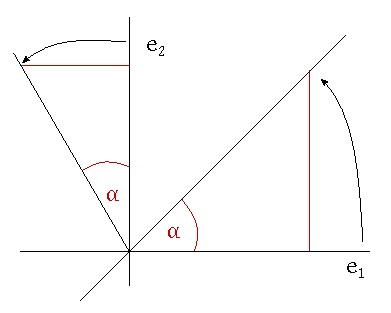
\includegraphics{img/13_rotation.pdf}
      \caption{Rotation in $\mathbb R^2$}
      \label{img:rotr2}
    \end{center}
  \end{figure}
\end{Example}

\begin{Example}[Rotation considered as motion]
  \begin{figure}[t]
    \begin{center}
      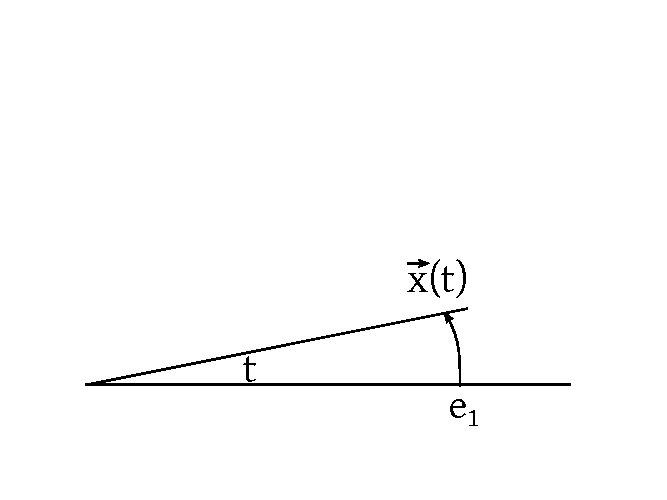
\includegraphics{img/14_rotation_as_motion.pdf}
      \caption{Rotation in $\mathbb R^2$ considered as motion. Commonly done by physicists.}
      \label{img:rotr2mot}
    \end{center}
  \end{figure}

  Tangent $a$:
  \[ \vectwo{x(t)}{y(t)} = \vectwo{\dot{x}(t)}{\dot{y}(t)} \]
  \[ \vec x(t) \bot \vec{x}(t) \]
  \[ \dot{\vec{x}}(t) = \begin{bmatrix} 0 & -1 \\ 1 & 0 \end{bmatrix} \vec{x}(t) \]
  \[ \vec{x}(t) = e^{\begin{bmatrix} 0 & -1 \\ 1 & 0 \end{bmatrix} t} \cdot \vec{x_0} \]
  Compare with Figure~\ref{img:rotr2mot}.

  \[ x'(t) = a\cdot x(t) \implies x(t) = c \cdot e^{at} \]
  \[ \frac{dx}{dt} = ax \]
  \[ dx = ax \cdot dt \]
  \[ \int \frac{dx}{x} = \int a \cdot dt \]
  \[ \log{x} = at + C \]
  \[ x = C_1 \cdot e^{at} \]

  \[ e^x = \sum_{n=0}^\infty \frac{x^n}{n!} \]
  \[ e^{\begin{bmatrix} 0 & -1 \\ 1 & 0 \end{bmatrix}t} = \sum_{n=0}^\infty \frac{\begin{bmatrix} 0 & -1 \\ 1 & 0 \end{bmatrix}^n}{n!} t^n \]
  \[ e^{it} = \cos{t} + i \cdot \sin{t} \]
  insert $\sum_{n=0}^\infty \frac{(it)^n}{n!}$ and split $\Re$ and $\Im$.

  \[ \begin{bmatrix} 0 & -1 \\ 1 & 0 \end{bmatrix}^2 = \begin{bmatrix} -1 & \\ & -1 \end{bmatrix} \]
  \[ \begin{bmatrix} 0 & -1 \\ 1 & 0 \end{bmatrix}^3 = \begin{bmatrix} 0 & -1 \\ 1 & 0 \end{bmatrix} \]
  \[ \begin{bmatrix} 0 & -1 \\ 1 & 0 \end{bmatrix}^4 = \begin{bmatrix} 1 &  \\  & 1 \end{bmatrix} \]

  \[ i^2 = -1 \qquad i^3 = -i \qquad i^4 = 1 \]

  \[
    e^{\begin{bmatrix} 0 & -1 \\ 1 & 0 \end{bmatrix} t} = \cos(t) \cdot \begin{bmatrix} 1 & \\ & 1 \end{bmatrix} + \sin(t) \cdot \begin{bmatrix} 0 & -1 \\ 1 & 0 \end{bmatrix} 
  \] \[
    U_{\alpha + \beta} = U_{\alpha} \cdot U_{\beta}
  \] \[
    \begin{bmatrix}
      \cos(\alpha + \beta) & -\sin(\alpha + \beta) \\
      \sin(\alpha + \beta) & \cos(\alpha + \beta)
    \end{bmatrix} =
    \begin{bmatrix}
      \cos\alpha & -\sin\alpha \\
      \sin\alpha & \cos\alpha
    \end{bmatrix} \cdot
    \begin{bmatrix}
      \cos\beta & -\sin\beta \\
      \sin\beta & \cos\alpha
    \end{bmatrix}
  \] \[
    =
    \begin{bmatrix}
      \cos\alpha \cos\beta - \sin\alpha \sin\beta & -\cos\alpha \cos\beta - \sin\alpha \sin\beta \\
      \sin\alpha \cos\beta + \cos\alpha \sin\beta & \sin\alpha \cos\beta + \cos\alpha \sin\beta
    \end{bmatrix}
  \]
\end{Example}

\begin{Example}[Reflection in $\mathbb R^2$]
  \[ S(e_1) = \begin{bmatrix} \cos(2\varphi) \\ \sin(2\varphi) \end{bmatrix} \]
  \[ S(e_2) = \begin{bmatrix} \cos(2\varphi - \frac\pi2) \\ \sin(2\varphi - \frac\pi2) \end{bmatrix} = \begin{bmatrix} \sin(2\varphi) \\ -\cos(2\varphi) \end{bmatrix} \]
  \[ \frac\pi2 - 2\psi = \frac\pi2 - 2\left(\frac\pi2 - \varphi\right) = 2\varphi - \frac\pi2 \]
  \[ S = \begin{bmatrix} \cos(2\varphi) & \sin(2\varphi) \\ \sin(2\varphi) & -\cos(2\varphi) \end{bmatrix} \]
\end{Example}

\dateref{2018/05/07}

Linear isometries:

\begin{theorem} % 8.73
  \begin{align*}
    \mathcal O(n) &= \setdef{U \in \mathbb R^{n\times n}}{U^TU = I} & \text{ orthogonal group} \\
    \mathcal U(n) &= \setdef{U \in \mathbb C^{n\times n}}{U^*U = I} & \text{ unitary group} \\
    \mathcal{SO}(n) &= \setdef{U \in \mathbb O}{\det(U) = 1} \subseteq \mathcal O(n) & \text{ subgroup, special orthogonal group} \\
    \mathcal{SU}(n) &= \setdef{U \in \mathbb U}{\det(U) = 1} \subseteq \mathcal U(n) & \text{ subgroup, special unitary group} \\
    \mathcal{GL}(n, \mathbb K) &= \setdef{A \in \mathbb K^{n\times n}}{\text{ invertible}} & \text{ general linear group} \\
    \mathcal{SL}(n, \mathbb K) &= \setdef{A \in \mathbb \mathcal{GL}(n)}{\det(A) = 1} & \text{ special linear group}
  \end{align*}
  Then, e.g. $\mathcal O(2)$ is the group of rotations and reflections.
\end{theorem}

\begin{Remark}
  For $U \in \mathcal U(n)$ it holds that $\card{\det(U)} = 1$. Why?

  We know: $U^* U = I \implies \det(U^* U) = I = \det(U^*) \det(U) = \det(\overline{U}^T) \det(U) = \overline{\det(U^T)} \det(U) = \overline{\det(U)} \det(U) = \card{\det(U)}^2 = 1$.
\end{Remark}

\begin{Example}[Rotation]
  \[ U = \begin{bmatrix} \cos{\varphi} & -\sin{\varphi} \\ \sin{\varphi} & \cos{\varphi} \end{bmatrix} \]
  \[ \det{U_{\varphi}} = \cos^2(\varphi) + \sin^2(\varphi) = 1 \qquad \implies U_{\varphi} \in \mathcal {SO}(2) \]
  \[ S_{\varphi} = \begin{bmatrix} \cos(2\varphi) & \sin(2\varphi) \\ \sin(2\varphi) & -\cos(2\varphi) \end{bmatrix} \]
  \[ \det(S_{\varphi}) = -\cos^2(2\varphi) - \sin^2(2\varphi) = -1 \]

  General orthogonal matrix in $\mathcal O(2)$.
  \[ U = \begin{bmatrix} a & b \\ c & d \end{bmatrix} \text{ with } \overline U U = \begin{bmatrix} 1 & 0 \\ 0 & 1 \end{bmatrix} \]
  \[
    \begin{bmatrix} a & c \\ b & d \end{bmatrix} \begin{bmatrix} a & b \\ c & d \end{bmatrix}
    = \begin{bmatrix} a^2 + c^2 & ab + cd \\ ab + cd & b^2 + d^2 \end{bmatrix}
    \overset!= \begin{bmatrix} 1 & 0 \\ 0 & 1 \end{bmatrix}
  \]
  Resulting constraints:
  \begin{align}
    a^2 + c^2 &= 1 \\
    b^2 + d^2 &= 1 \\
    ab + cd &= 0
  \end{align}
  \[ a = \cos\varphi \qquad c = \sin\varphi \qquad b = \cos\psi \qquad d = \sin\psi \]
  \[ \cos\varphi \cdot \cos\psi + \sin\varphi \cdot \sin\psi = 0 \]
  \[
    \begin{bmatrix} \cos\alpha & -\sin\alpha \\ \sin\alpha & \cos\alpha \end{bmatrix}
    \begin{bmatrix} \cos\beta & -\sin\beta \\ \sin\beta & \cos\beta \end{bmatrix}
    = \begin{bmatrix}
      \cos(\alpha + \beta) \\
    \end{bmatrix}
  \]
  \[ \cos \alpha \cos \beta - \sin \alpha \sin \beta = \cos(\alpha + \beta) \]
  \[ \cos \varphi \cdot \cos \psi = \cos(\varphi - \psi) \]
  \[ \cos \alpha = 0 \text{ for } \alpha = \frac\pi2 + k \cdot \pi = (k + \frac12) \pi \qquad (k \in \mathbb Z) \]
  \[ \implies \varphi - \psi = (k + \frac12) \pi \]
  \[ \varphi = \psi + (k + \frac12) \pi \]
  \begin{align*}
    \cos\varphi &= \cos(\psi + (k + \frac12) \pi) = \cos\psi \cos(k + \frac12) \pi - \sin\psi \underbrace{\sin(k + \frac12) \pi}_{\varepsilon \in \set{\pm 1}} \\
       &= -\varepsilon \cdot \sin\psi \implies \sin\psi = -\varepsilon \cos\varphi
  \end{align*}
  \[ \sin\alpha \cos\beta + \cos\alpha \sin\beta = \sin(\alpha + \beta) \]
  \[ \sin(\varphi) = \sin(\psi + (k + \frac12) \pi) = \underbrace{\sin\psi \cos\left(k + \frac12\right) \pi}_{= \varepsilon \cdot \cos(\psi)} + \underbrace{\cos \psi \sin \left(k + \frac12\right) \pi}_{= 0} \]
  \[ \cos\psi = \varepsilon \sin\varphi \]
  \[
    U = \begin{bmatrix} \cos\varphi & \varepsilon \cdot \sin(\psi) \\ \sin\varphi & -\varepsilon \cos\varphi \end{bmatrix}
    = \underbrace{\begin{bmatrix} \cos\varphi & -\sin\varphi \\ \sin\varphi & \cos\varphi \end{bmatrix}}_{\substack{\text{rotation} \\ \det = 1}} \cdot \underbrace{\begin{bmatrix} 1 & \\ & -\varepsilon \end{bmatrix}}_{\substack{\varepsilon = 1: \\ \text{reflection on x-axis} \\ \varepsilon = -1: \operatorname{id}}}
  \] \[
    U_{\varphi} = \cos\varphi \begin{bmatrix} 1 & \\ & 1 \end{bmatrix} + \sin\varphi \begin{bmatrix} & -1 \\ 1 & \end{bmatrix}
  \]
  Hence, every orthogonal matrix is either a rotation ($\det = 1$) or a reflection ($\det = -1$).

  \[ \mathcal{SO}(2): \set{U_{\varphi} = \cos\varphi + i \cdot \sin\varphi \qquad 1 = \begin{bmatrix} 1 & 0 \\ 0 & 1 \end{bmatrix}, i = \begin{bmatrix} 0 & -1 \\ 1 & 0 \end{bmatrix}} \]
  \[ \mathcal{SU}(2): \setdef{a_0 + i a_1 + j a_2 + k a_3}{\sum a_i^2 = 1} \]
\end{Example}

\subsection{Quaternions}

\begin{Person}
  William Rowan Hamilton (1805--1865).
\end{Person}

\index{Quaternions}
\index{Complex numbers}
\begin{Remark}[Quaternions]
  Hamilton defined the complex numbers in the modern sense in 1833.
  \[ \mathcal C = \setdef{(a,b)}{a,b \in \mathbb R} \]
  \[ (a,b) \cdot (c, d) = (ac - bd, ad + bc) \]
  He tried to invent them over 10 years for the third dimension.
  He failed.
  On 1843/10/16, he invented the quaternions (a memorial next to Brougham Bridge in Dublin reminds of the moment of discovery).
  It works on four dimensions, but it is non-commutative.
  It is a screw field (dt.~\foreignlanguage{german}{Schiefk\"orper}).
  \[ ij = k \qquad jk = i \qquad ki = j \qquad ji = -k \qquad kj = -i \qquad ik = -j \]
  anti-commutative.
  \[ i^2 = j^2 = k^2 = -1 \]
  \[ (a_0 + a_1 i + a_2 j + a_3 k) (b_0 + b_1 i + b_2 j + b_3 k) \qquad \text{ linear} \]
  \[ (a_0 + \vec a) (b_0 + \vec b) = a_0 b_0 + a_0 \vec b + b_1 \vec a + \vec a \times \vec b \]
\end{Remark}

\[ \mathcal{SO}(2) \eqsim \setdef{\cos\varphi + i \cdot \sin\varphi}{\varphi \in [0,2\pi]} = \setdef{z \in \mathbb C}{\card{z} = 1} = \mathcal T \text{ Torus} \]
\[ \mathcal{SU}(2) = \setdef{a_0 + i a_1 + j a_2 + k a_3}{\sum a_i^2 = 1} \]
\[ \mathcal{SO}(2) \eqsim \setdef{\cos \varphi + i \sin\varphi}{q \in [0,2\pi]} \]

\section{Polynomials and algebras} % Chapter 9

\index{Algebra}
\begin{definition}[Algebra] % definition 9.1
  Let $\mathbb K$ be a field, a $\mathbb K$ algebra is a vector space $\mathcal A$ over $\mathbb K$
  with a multiplication operator $*: \mathcal A \times \mathcal A \to \mathcal A$ with $(a,b) \to a * b$ such that
  \begin{enumerate}
    \item $a * (b + c) = a * b + a * c$ (distributive law, $a, b, c \in \mathcal A$)
    \item $(a + b) * c = a * c + b * c$
    \item $\lambda \cdot (a * b) = (\lambda \cdot a) * b = a * (\lambda \cdot b)$ ($a, b \in \mathcal A, \lambda \in \mathbb K$, associativity)
  \end{enumerate}
\end{definition}

\index{Associative algebra}
\index{Commutative algebra}
\begin{remark} % Bemerkung 9.2
  \begin{description}
    \item[Associativity] is not generally required.
      \[ a * (b * c) = (a * b) * c \]
      If satisfied, it is called \emph{associative algebra}.
    \item[Commutativity] is not generally required.
      \[ a * b = b * a \]
      If satisfied, it is called \emph{commutative algebra}.
  \end{description}
\end{remark}

\index{Jacobian identity}
\index{Commutator}
\index{Lie algebra}
\index{Lie groups}
\index{Jordan algebra}
\begin{example} % Beispiel 9.3
  \begin{enumerate}
    \item $(\mathbb K, +, * = \cdot)$ is a one-dimensional $\mathbb K$ algebra.
    \item $(\mathbb K^{n \times n}, +, * = \text{ matrix multiplication})$ is an associative non-commutative algebra
      where $\mathbb K^{n \times n} \simeq \Hom(V, V)$ and $f * g = f \circ g$.
    \item $\mathbb K^\times = \set{f: X \to \mathbb K}$. Let $X$ be an arbitrary set.
      \[ (\lambda f + \mu g)(x) = \lambda \cdot f(x) + \mu \cdot g(x) \]
      \[ (f * g)(x) = f(x) \cdot g(x) \]
      $(\mathbb K^\times, +, *)$ is an associative, commutative algebra.
    \item $\mathbb R^3$ with $a \times b$ is an algebra.
      \[ a \times b = -b \times a \]
      is non-commutative and also non-associative:
      \[ a \times (b \times c) \neq (a \times b) \times c \]
      Jacobian identity:
      \[ a \times (b \times c) + b \times (c \times a) + c \times (a \times b) = 0 \]
    \item $\mathcal A = \mathbb K^{n\times n}$
      \[ A * B = [A,B] = A \cdot B - B \cdot A \qquad \text{\enquote{commutator}} \]
      is an algebra with Jacobian identity. Lie algebra:
      \[ [A, [B,C]] + [B, [C,A]] + [C, [A,B]] = 0 \]
      \[ [A,B] = -[B,A] \]
      The so-called Lie groups (like $\mathcal O(n), \mathcal U(n), \mathcal{SO}(n), \mathcal{SU}(n)$).
    \item
      $\mathcal A = \mathbb K^{n\times n}$
      \[ A * B = A \cdot B + B \cdot A \]
      is associative. It is an Jordan algebra.
  \end{enumerate}
\end{example}

\begin{Person}
  Pascual Jordan (1902--1980)\footnote{Different Jordan than in Gauss-Jordan and different than C. Jordan (19th century) about to come}.
\end{Person}

\begin{Person}
  Oskar Perron (1880/05/07--1975)
\end{Person}

\index{Cauchy product}
\begin{definition} % Definition 9.4
  \[ \mathbb K^\infty = \setdef{(a_0, a_1, a_2, \dots)}{a_i \in \mathbb K} \]
  \[ P_{\mathbb K} = \setdef{(a_0, a_1, \dots, a_n, 0, \dots)}{n \in \mathbb N, a_i \in \mathbb K} \]
  We define $*$ as the Cauchy product:
  \[ (a_n)_{n \geq 0} * (b_n)_{n \geq 0} = (c_n)_{n \geq 0} \qquad c_n = \sum_{k=0}^n a_k b_{n-k} \]
\end{definition}

\index{Polynomial algebra}
\index{Formal power series algebra}
\begin{lemma} % Lemma 9.5
  \label{lemma95}
  \begin{enumerate}
    \item $(P_{\mathbb K}, *)$ is a commutative, associative algebra with one-element $(1, 0, \dots)$.
      The basis is given with $1, x, x^2, \dots$. The algebra is called \emph{polynomial algebra}
      \[ \mathbb K[x] = \setdef{\sum_{k=0}^n a_k x^k}{a_k \in \mathbb K, n \in \mathbb N} \]
    \item $(\mathbb K^\infty, *)$ is a commutative algebra with one-element $(1, 0, \dots)$
      and is called \emph{algebra of formal power series}\footnote{We don't need to consider convergence. This is purely formal object.}
      \[ \mathbb K[[x]] = \setdef{\sum_{k=0}^\infty a_k x^k}{a_k \in \mathbb K} \]
  \end{enumerate}
\end{lemma}

\begin{proof}
  We show algebra properties:
  \begin{enumerate}
    \item 
      Show that $\forall a,b \in P_{\mathbb K}: a * b \in P_{\mathbb K}$, hence only finitely many $c_n$ are $\neq 0$.

      Remark: $a_k = 0 \forall k > m$ and $b_k = 0 \forall k > n$.
      \begin{claim}
        \[ c_k = 0 \qquad \forall k > m + n \]
      \end{claim}%
      \begin{align*}
        c_k &= \sum_{l=0}^k a_l b_{k-l} \\
            &= \sum_{l=0}^{m-1} a_l b_{k-l} \qquad \text{equality if $l > m \implies a_l = 0$} \\
            &= 0
      \end{align*}
      \[ k > m + n, l < m \implies -l > -m \implies k - l \underbrace{>}_{\implies b_{k-l} = 0} m + n - m = n \]
    \item
      About the Cauchy product:
      \[ c_n = \sum_{k=0}^n a_k b_{n-k} = \sum_{k'=0}^n a_{n-k'} b_{k'} = (b * a)_n \qquad (k' = n - k) \]

    \item
      Law of distributivity:
      \begin{align*}
        [(a + b) * c]_n &= \sum_{k=0}^n (a + b)_k \cdot c_{n-k} \\
          &= \sum_{l=0}^n (a_k c_{n-k}) + (b_k c_{n-k}) \\
          &= (a * c)_n + (b * c)_n
      \end{align*}
  \end{enumerate}
\end{proof}

\index{Basis of a polynomial}
\index{Degree of a polynomial}
\begin{definition} % Definition 9.6
  Let $x^0 = (1, 0, \dots)$ and $x^k = (0, \dots, 1, 0, \dots)$ create a basis.
  The elements of $p(x) = \mathbb K[x]$ are called polynomials in the formal variable $x$
  \[ \deg{p(x)} = \max\setdef{k}{a_k \neq 0} \text{ is called \emph{degree of the polynomial}} \]
  \[ \deg(0) \coloneqq -\infty \]
\end{definition}

\begin{lemma}\hfill{} % Lemma 9.7
  \begin{enumerate}
    \item $\deg(p(x) \cdot q(x)) = \deg(p(x)) + \deg(q(x))$
    \item $\mathbb K[x]$ is zero-divisor-free,
      hence $p(x) \cdot q(x) = 0 \implies p(x) = 0 \lor q(x) = 0$
  \end{enumerate}
\end{lemma}

\subsection{The difference of polynomials and polynomial functions}

\index{Polynomial function}
\begin{definition} % Definition 9.8
  Every polynomial $p(x) \in \mathbb K[x]$ induces a polynomial function $p: \mathbb K \to \mathbb K$ with $\alpha \mapsto p(\alpha)$
  with $p \in \mathbb K^{\mathbb K}$.
  \[ \implies (\lambda p + \mu q) (\alpha) = \lambda \cdot p(\alpha) + \mu \cdot q(\alpha) \]
  \[ (p \cdot q)(\alpha) = p(\alpha) \cdot q(\alpha) \]
  The map $\mathbb K[x] \to \mathbb K^{\mathbb K}$ with $p(x) \mapsto$ polynomial function $p$
  is linear and multiplicative (called \emph{algebra homomorphism}).
\end{definition}

\begin{remark} % Bemerkung 9.9
  A polynomial and a polynomial function are not the same.
  If $\card{\mathbb K} < \infty$, a difference occurs.
  For example, consider $\mathbb Z_5$:
  \[ \card{\mathbb Z_5^{\mathbb Z_5}} = 5^5 \]
  \[ \card{\mathbb K[x]} = \infty \]
  where $\mathbb Z_5^{\mathbb Z_5}$ is a set of polynomial functions and $\mathbb K[x]$ is a set of polynomials.
  For example, $\prod_{\alpha \in \mathbb K}(x - \alpha)$ corresponds to the polynomial function $0$.
  Consider $\mathbb K = \mathbb Z_3$. If $\alpha \in \mathbb Z_3$ and $x \in \mathbb Z_3$, we get $(x - 0)(x - 1)(x - 2)$
  and choosing any $x \in \mathbb Z_3$ makes at least one factor zero. Thus, the polynomial function $0$ is given.
  Hence the map $\mathbb K[x] \to \mathbb K^{\mathbb K}$ is surjective but not injective.

  On finite fields, every function is a polynomial function.
  \[ \eta_i = f(\xi_i) \qquad \set{\xi_1, \dots, \xi_n} = \mathbb K \]
  From the practicals, it will follow that there exists a polynomial of degree $n$ such that $p(\xi_i) = \eta_i$.
\end{remark}

\index{Algebra homomorphism}
\begin{definition} % Definition 9.10
  An algebra homomorphism is a linear map between $\psi$ and two $\mathbb K$-algebras $\mathcal A$ and $\mathcal B$ such that
  $\forall a,b \in \mathcal A: \psi(a *_A b) = \psi(a) *_B \psi(b)$.
\end{definition}

\begin{example} % Beispiel 9.11
  \begin{enumerate}
    \item $\mathbb K[x] \to \mathbb K^{\mathbb K}$ with $p(x) \mapsto$ polynomial function
    \item
      Let $\alpha \in \mathbb K$ be fixed.
      $\psi_{\alpha}: \mathbb K[x] \to \mathbb K$ with $p(x) \mapsto p(\alpha)$ is an algebra homomorphism of $\mathbb K[x] \to \mathbb K$.
      \[ \psi_\alpha(\lambda p + \mu q) = (\lambda p + \mu q)(\alpha) = \lambda p(\alpha) + \mu q(\alpha) = \lambda \psi_{\alpha}(p) + \mu \psi_{\alpha}(q) \]
    \item Consider $\iota: \mathbb K \to \mathbb K[x]$ with $\iota: \alpha \mapsto \alpha \cdot x^0$.
      \[ (\alpha \cdot x^0) \cdot (\beta \cdot x^0) = (\alpha \cdot \beta) \cdot x^0 \]
  \end{enumerate}
\end{example}

\begin{theorem}[Insertion theorem, dt. \foreignlanguage{german}{Einsetzungssatz}] % Satz 9.12
  Let $\mathcal A$ be an associative algebra with one-element $\mathbf 1_A$
  and $\iota: \mathbb K \to \mathcal A$ with $\alpha \mapsto \alpha \cdot \mathbf 1_A$ is the insertion of $\mathbb K$.

  Then for every $a \in \mathcal A$ the map
  \[ \psi_a: \mathbb K[x] \to \mathcal A \]
  \[ \sum_{k=0}^n c_k x^k \mapsto \sum_{k=0}^n c_k a^k \]
  is the unique algebra homomorphism of $\mathbb K[x] \to \mathcal A$ with the property $\psi_a(x) = a$.
  We say, $\mathbb K[x]$ is a \emph{free, associative algebra over $\mathbb K$}.
  Every algebra homomorphism $\mathbb K[x] \to \mathcal A$ has this structure.
\end{theorem}

\dateref{2018/05/09}

We consider algebras as vector spaces with associative multiplication. For example, matrices and polynomials.
An algebra homomorphism is linear and multiplicative.
\[ \Phi(a + b)= \Phi(a) * \Phi(b) \]
$A$ is an associative algebra with $\mathbf 1_{\mathcal A}$.
\[ l: \begin{array}{cc} \mathbb K \to \mathcal A \\ \alpha \to \alpha \cdot \mathbf 1_{\mathcal A} \end{array} \]
$a \in \mathcal A \implies \mathcal L(a^0, a^1, a^2, a^3, \dots) \subseteq \mathcal A$ subalgebra.

\begin{enumerate}
  \item Show linear and multiplicative property.
    \[ \exists! \Phi_a: \mathbb K[a] \to \mathcal A \text{ algebra homomorphism} \]
    such that $\Phi_a(x) = a$, namely $\Phi_a\left(\sum_{k=0}^n c_k x^k\right) = \sum_{k=0}^n c_k a^k$.
  \item
    Every homomorphism $\Psi: \mathbb K[x] \to \mathcal A$ has this structure.
    \begin{proof}
      Let $a \coloneqq \Psi(x) \implies \Psi(x^n) = \Psi(x)^n = a^n$ by homomorphism.
      \[ \Psi \text{ linear } \implies \Psi\left(\sum_{k=0}^n c_k x^k\right) = \sum_{k=0}^n c_k \Psi(x^k) = \sum_{k=0}^n c_k a^k \]
      $x^0, x^1, \dots$ give a basis of $\mathbb K[x]$.
      Hence $\Psi = \Phi_a$ with $a = \Psi(x)$. On the opposite (1.): Obviously $\Phi_a$ is linear.
      Multiplicative: Show that
      \[ \underbrace{\Psi_a(p(x) \cdot q(x))}_{= p(a) \cdot q(a)} \overset!= \underbrace{\Phi_a(p(x)) \cdot {}_{\mathcal A}\Phi_a(q(x))}_{= p(a) \cdot q(a)} \]
    \end{proof}
\end{enumerate}

\begin{example} % Beispiel 9.13
  \begin{enumerate}
    \item $\mathcal A = \mathbb K$.
      \[ \Psi_\alpha: \substack{\mathbb K[x] \to \mathbb K \\ p(x) \mapsto p(\alpha)} \]
    \item $\mathcal A = \mathbb K^{n\times n} \eqsim \Hom(V, V)$
      \[ A^0 = I \qquad A^n = A \cdot A^{n-1} \]
      \[ l: \substack{\mathbb K \to \mathbb K^{n\times n} \\ \alpha \mapsto \alpha \cdot I} \]
      \[ \Psi_\alpha: \substack{\mathbb K[x] \to \mathbb K^{n\times n} \\ p(x) \mapsto p(A) \\ \sum_{k=0}^n c_k x^k \mapsto \sum_{k=0}^n c_k \cdot A^k}  \]
  \end{enumerate}
\end{example}

\begin{remark} % Bemerkung 9.14
  Let $\mathbb K[x]$ be a free, associative algebra over $\mathbb K$ with a generator.
  Hence, for all associative algebras $\mathcal A$, given some element $a \in \mathcal A$.
  There exists exactly one homomorphism $\varphi: \mathbb K[x] \to \mathcal A$ such that $\varphi(x) = a$.

  Compare it with a free group with one generator. Is a group $G$ generated by $x$ such that $\forall$ groups $H$, if $h \in H$ given,
  there exists exactly one group homomorphism $\varphi: G \to H$ such that $\varphi(x) = h$. Namely, $G = (\mathbb Z, +)$ is generated by $\mathbf 1$.
  Given $h \in H \to \varphi_h: \mathbb Z \to H_k$ and $k \mapsto h$.
\end{remark}

\index{Root of a polynomial}
\begin{definition}
  A \emph{root of a polynomial} $p(x) \in \mathbb K[x]$ is a $\xi \in \mathbb K$ such that $p(\xi) = \Psi_{\xi}(p) = 0$,
  hence $p(x) \in \ker{\Psi_{\xi}}$.
\end{definition}

\begin{Remark}
  \begin{enumerate}
    \item $p(x) = c_0 \text{ is a root } \iff c_0 = 0$
    \item $p(x) = c_0 + c_1 x$ is the only root, $\xi = -\frac{c_0}{c_1}$.
    \item $p(x) = c_0 + c_1 x + c_2 x^2$ has two roots over $\mathbb C$
    \item $p(x) = c_0 + c_1 x + c_2 x^2 + c_3 x^3$ has three roots
  \end{enumerate}

  To find roots, formulas up to fourth degree exist.
  For degree $\geq 5$, there is no equation.
\end{Remark}

\begin{Person}
  Paolo Ruffini (1765--1822)
\end{Person}
\begin{Person}
  Niels Henrik Abel (1802--1829)
\end{Person}
\begin{Person}
  Gerolamo Cardano (1501--1576)
\end{Person}

\begin{Remark}
  Cardano was a polymath.
  \begin{itemize}
    \item founder of probability theory
    \item \emph{Liber de ludo aleae}: important book on probability
    \item Cardan joint (dt. \foreignlanguage{german}{Kardanische Welle})
    \item Gimbal (dt. \foreignlanguage{german}{Kardanische Aufh\"angung})
    \item used $\sqrt{-1}$ as a valid expression for the first time
    \item published a solution for roots of cubic polynomials (Ars Magna, 1545)
  \end{itemize}

  \begin{Person}
    Scipione del Ferro (1465--1526)
  \end{Person}

  \begin{itemize}
    \item used a solution for roots of cubic polynomials in competitions, kept it secret
    \item came up with the same solution like Tartaglia
    \item lost competitions on cubic polynomials to Antonio Fiore, because Ferro's solution was not generic enough
  \end{itemize}

  \begin{Person}
    Niccol\`o Fontana Tartaglia (1500--1557)
  \end{Person}

  \begin{enumerate}
    \item Cardano cajoled Tartaglia into revealing his solution to the cubic equations by promising not to publish them.
  \end{enumerate}

  \begin{Person}
    Ludovico Ferrari (1522--1565)
  \end{Person}
\end{Remark}

\begin{Person}
  Vi\`ete, Francois (1540--1603)
\end{Person}

\index{Method by Cardano/del Ferro}
\begin{theorem}[Method by Cardano/del Ferro] % 9.16
  \[ a_0 + a_1 x + a_2 x^2 + a_3 x^3 = 0 \]
  \[ x \to x + a \qquad \text{ such that } a_2 = 0 \]

  \[ x^3 + px + q = 0 \]
  Cubus p.6 rebus aeq 20 \\
  $x^3 + 6x = 20$

  $x = $ res, $x^2 = $ census, $x^3 = $ cubus.

  Approach: $x = u + v$.

  \[ u^3 + 3u^2v + 3uv^2 + v^3 + p(u + v) + q = 0 \]
  \[ u^3 + v^3 + (3uv + p)(u + v) + q = 0 \]

  Requirement:
  $u$ and $v$ such that $3uv + p = 0$.

  \[
    \begin{cases}
      u^3 + v^3 + q = 0 & \implies v^3 = -(q + u^3) \\
      3uv + p = 0 & \implies uv = -\frac{p}{3u}
    \end{cases}
  \]
  \[ u^3 \cdot v^3 = -\frac{p^3}{27} \]
  \[ -u^3 (q + u^3) = -\frac{p^3}{27} \]
  \[ u^6 + qu^3 - \frac{p^3}{27} = 0 \]
  \[ u^3 = ? \]

  Equation for degree 2 by Vi\`ete Francois:

  \[ (y - \alpha)(x - \beta) = x^2 - (\alpha + \beta) x + \alpha \beta \]
  \[ x^2 + px + q \]
  \[ p = -(\alpha + \beta) \]
  \[ q = \alpha \cdot \beta \]

  \[ \alpha = \frac12 \left[(\alpha + \beta) + \sqrt{(\alpha - \beta)^2}\right] \]
  \[ \beta = \frac12 \left[(\alpha + \beta) - \sqrt{(\alpha - \beta)^2}\right] \]
  \[
    \frac\alpha\beta = \frac12 \left(\alpha + \beta \pm \sqrt{(\alpha - \beta)^2}\right)
    = \frac12 \left(\alpha + \beta \pm \sqrt{\underbrace{\alpha^2 + \beta^2 - 2\alpha\beta}_{(\alpha + \beta)^2 - 4\alpha\beta}}\right)
    = \frac12 \left(-p \pm \sqrt{p^2 - 4q}\right)
  \]

  Hence,
  \begin{align*}
    u^3 &= \frac12\left(-q \mp \sqrt{q^2 + \frac{4p^3}{27}}\right) \\
    u^3 &= \frac{q}2 \pm \sqrt{\frac{q^2}{4} + \frac{p^3}{27}} \\
    u &= \sqrt[3]{-\frac{q}2 \pm \sqrt{\frac{q^2}{4} + \frac{p^3}{27}}} \\
    v^3 &= -q - u^3 = -\frac{q}{2} \mp \sqrt{\frac{q^2}{4} + \frac{p^3}{27}} \\
    x = u + v &= \sqrt[3]{-\frac{q}2 + \sqrt{\frac{q^2}{4} + \frac{p^3}{27}}} + \sqrt[3]{-\frac{q^2}{2} - \sqrt{\frac{q^2}{4} + \frac{p^3}{27}}}
  \end{align*}
\end{theorem}

\index{Polynomial division}
\begin{theorem}[Division with remainder] % 9.17 Satz
  $p(x), q(x) \in \mathbb K[x]$, $q(x) \neq 0$.

  Then there exists exactly one polynomial $s(x), r(x) \in \mathbb K[x]$,
  \[ p(x) = s(x) \cdot q(x) + r(x) \]
  with $\deg{r(x)} < \deg{q(x)}$.
\end{theorem}

\begin{proof}
  Induction over $\deg{p(x)}$.
  \begin{description}
    \item[Induction base]
      \[ \deg{p(x)} < \deg{q(x)} \leadsto p(x) = 0 \cdot q(x) + p(x) \]
      If $\deg{p(x)} \geq \deg{q(x)}$,
      \[ p(x) = \sum_{k=0}^n a_k x^k \qquad q(x) = \sum_{k=0}^m b_k x^k  \]
      \[ a_n \neq 0 \qquad m \leq n \qquad b_m \neq 0 \]

      \begin{align*}
        p_1(x) &= p(x) - \frac{a_n}{b_m} \cdot q(x) \cdot x^{n-m} \
      \intertext{cancels the largest term $a_n x^n$ in $p(x)$.}
          &= \sum_{k=0}^n a_k x^k - \frac{a_n}{b_m} \sum_{k=0}^m b_k x^{k+n-m} \\
          &= a_n x^n + \sum_{k=0}^{n-1} a_k x^k - \frac{a_n}{b_m} b_m \cdot x^{m+n-m} - \frac{a_n}{b_m} \sum_{k=0}^{m-1} b_k x^{k+n-m} \\
      \end{align*}
      what remains is a polynomial of degree $\deg{p_1(x)} \leq n-1$.
      \[ \implies p(x) = \frac{a_n}{b_m} x^{n-m} \cdot q(x) + p_1(x) \]
      By induction hypothesis,
      \[ p_1(x) = s_1(x) \cdot q(x) + r_1(x) \]
      Hence,
      \[ p(x) = \left(\frac{a_n}{b_m} x^{n-m} + s_1(x)\right) q(x) + r_1(x) \]
  \end{description}
\end{proof}

\begin{example} % Beispiel 9.18
  \begin{align*}
    p(x) &= 3x^5 - x^4 + 2x^3 + x^2 + 1 \\
    q(x) &= x^2 - 3x + 1 \\
  \end{align*}
  \[
    \begin{array}{rrrrrrl}
      3x^5 &- x^4 &+ 2x^3 &+ x^2 & &+ 1 &: x^2 - 3x + 1 = 3x^2 + 8x^2 + 23x + 62 \\
      -3x^5 & +9x^4 & -3x^3 \\
      \cline{1-3}
      0 & 8x^4 & -x^3 & +x^2 & & +1 \\
        & 8x^4 & -24x^3 & +8x^2 \\
      \cline{2-6}
        & 0 & 23x^3 & -7x^2 & & +1 \\
        &   & 23x^3 & -69x^2 & +23x \\
      \cline{3-6}
        &   & 0     & 62x^2 & -23x & +1 \\
        &   &       & 62x^2 & -186x & +62 \\
      \cline{4-6}
        &   &       & 0     & 163x & -61
    \end{array}
  \]
  Hence, $s(x) = 3x^3 + 8x^2 + 23x + 62$ and $r(x) = 163x - 61$.
\end{example}

\begin{definition} % 9.19
  $q(x)$ \emph{divides} $p(x) \iff $ the remainder is zero
  $\iff$ there exists $s(x)$ such that $p(x) = s(x) \cdot q(x)$.
\end{definition}

\begin{theorem} % Satz 9.20
  \begin{enumerate}
    \item If $p(x) = s(x) \cdot (x - \xi) + r$, then $q(x) = x - \xi$ with $p(\xi) = r$.
    \item $\xi$ is root of $p(x) \iff x - \xi$ divides $p(x)$
  \end{enumerate}
\end{theorem}

\begin{theorem}[Ruffini-Horner's method]
  Given $p(x) \in \mathbb K[x]$, $\lambda \in \mathbb K$. \\
  Find $p(\lambda)$.
  \begin{align*}
    p(x) &= a_n x^n + a_{n-1} x^{n-1} + \dots + a_1 x + a_0 \\
      &= a_n \lambda^n + a_{n-1} \lambda^{n-1} + \ldots + a_1 \lambda + a_0 \\
      &= \left(a_n \lambda^{n-1} + \dots + a_n\right) \lambda + a_0 \\
      &= \left((a_n \lambda^{n-2} + \dots + a_n) \lambda + a_1\right) \lambda + a_0 \\
      &= \vdots
  \end{align*}

  Algorithm:
  \[ \xi_n = a_n \text{ for } k = n-1, \dots, 0 \qquad \xi_k = \lambda \xi_{k+1} + a_k \]
  \[ p(\lambda) = \xi_0 \]
  If $p(x) = s(x) (x - \lambda) + r$, $p(\lambda) = r$.

  Horner's method provides a more convenient method to evaluate a polynomial for given $x$
  than exponentiation by a high degree.
\end{theorem}

\begin{example} % Beispiel 9.22
  \[ 3x^5 - x^4 + 2x^3 + x^2 + 1 \]
  \[ p(5) = ? \qquad \xi_5 = 3 \]
  \[
    \begin{vmatrix}
      3x^5 & -x^4 & +2x^3 & +x^2 & +1 & : (x - 5) & = & 3x^4 + 14x^3 + 72x^2 + 361x + 1805 \\
      3x^5 & -15x^4 \\
      0    & 14x^4 & +2x^3 & +x^2 & +1 \\
           & 14x^4 & -70x^3 & \\
           & 0     & +72x^3 & +x^2 & +1 \\
           &       & 72x^3 & -360x^2 \\
           &       & 0     & +361x^2 & +1 \\
           &       &       & 361x^2 & -1805x \\
           &       &       &        & 1805x & +1 \\
           &       &       &        & 1805x & -5 \cdot 1805 \\
           &       &       &        &       & 5 \cdot 1805+1
    \end{vmatrix}
  \]
  \[ \xi_5 = 3 \]
  \[ \xi_4 = 5 \cdot \xi_5 + (-1) = 5 \cdot 3 - 1 = 14 \]
  \[ \xi_3 = 5 \cdot 14 + 2 = 72 \]
  \[ \xi_2 = 5 \cdot 72 + 1 = 361 \]
  \[ \xi_1 = 5 \cdot 361 + 0 = 1805 \]
  \[ \xi_0 = 5 \cdot 1805 + 1 = 9026 \]
\end{example}

\index{Reducible polynomial}
\index{Irreducible polynomial}
\index{Factorization of a polynomial}
\begin{definition} % 9.23
  A polynomial $p(x) \in \mathbb K[x]$ is called \emph{reducible},
  if $\exists p_1(x), p_2(x): \deg{p_1(x)} < \deg{p(x)}$ and $p(x) = p_1(x) \cdot p_2(x)$ (is the factorization).
  $\deg{p_2(x)} < \deg{p(x)}$ (proper divisor).
  Otherwise the polynomial is called \emph{irreducible}.
\end{definition}

\begin{remark} % Bemerkung 9.24
  An irreducible polynomial of degree $>1$ has no roots.
\end{remark}

\begin{example} % Beispiel 9.25
  \begin{itemize}
    \item
      Consider $x^2 = -2$ irreducible over $\mathbb Q \subseteq \mathbb R \subseteq \mathbb R$.
      Its roots are $\pm \sqrt2$.

      It is reducible over $\mathbb R$: $x^2 - 2 = (x - \sqrt2)(x + \sqrt2)$. \\
      It is reducible over $\mathbb Q(\sqrt{2}) = \setdef{a + b\sqrt{2}}{a,b \in \mathbb Q}$.
    \item
      Consider $x^2+1$ irreducible over $\mathbb Q, \mathbb R$ and reducible over $\mathbb C$.
      Its roots are $\pm i$.

      $\mathbb Q(i) = \setdef{a + bi}{a,b \in \mathbb Q}$.
      $x^2 + 1 = (x + i)(x - i)$.
    \item
      Consider $\mathbb K = \mathbb Z_2$ and $p(x) = x^2 + x + 1$.
      This polynomial has no roots and is irreducible.
    \item
      $x^5 + x + 1$ has no roots, is reducible.
      \[ x^5 + x + 1 = (x^2 + x + 1)(x^3 + x^2 + 1) \]
      Is there some field $\mathbb K \supseteq \mathbb Z_2$ such that $x^3 + x^2 + 1$ has roots?

      \underline{Yes}. Let $\alpha$ be a number such that $\alpha^3 + \alpha^2 + 1 = 0 \implies \alpha^3 = -\alpha^2 - 1 = \alpha^2 + 1$.
      \[ \mathbb K = \mathbb Z_2(\alpha) = \setdef{a + b\alpha + c\alpha^2}{a,b,c \in \mathbb Z_2} \]
      with $\alpha^3 = \alpha^2 + 1$ is a field.

      Let $i$ be a number such that $i^2 + 1 = 0$, thus $i^2 = -1$
      \[ \mathbb C = \mathbb R(i) = \setdef{a + bi}{a,b \in \mathbb R} \]
  \end{itemize}
  Hence, irreducible is not equivalent to some root exists.
  The implication works only in one direction.
  There always exists some field such that roots exist.
\end{example}

\begin{theorem}[Fundamental theorem of Algebra] % Satz 9.26
  $\mathbb C$ is algebraically closed, hence every polynomial has a root over $\mathbb C$.
\end{theorem}

\begin{corollary}
  Every polynomial over $\mathbb C$ \dots
  \begin{enumerate}
    \item has a factorization $p(x) = (x - \xi_1) (x - \xi_2) \dots (x - \xi_n)$.
    \item $p(x)$ is irreducible $\iff \deg{p(x)} \leq 1$.
  \end{enumerate}
\end{corollary}
\begin{Remark}
  No algebraic proof exists. It is more like a Fundamental Theorem of Calculus over complex numbers.
  The proof is given by the Lionville theorem (not done here).
\end{Remark}

\begin{theorem} % Satz 9.27
  For arbitrary fields, it holds that
  every polynomial has exactly one factorization (except for its order) in irreducible factors.
\end{theorem}

\dateref{2018/05/14}

\subsection{The greatest common divisor of polynomials}

The Euclidean algorithm determines the greatest common divisor.

Consider $n = q \cdot m + r$. For the Euclidean algorithm, it holds that $\operatorname{gcd}(n, m) = \operatorname{gcd}(m, r)$
The analogous solution holds for polynomials. Consider $p(x) = s(x) \cdot q(x) + r(x)$.
Then the $\operatorname{gcd}(p(x), q(x))$ returns the polynomial of maximum degree that divides the polynomial with leading coefficient $1$.

\begin{corollary}
  The Euclidean algorithm also works for polynomials.
\end{corollary}

An application: Find all multiple roots (i.e. roots with multiplicity greater 1).
\[ (x - \xi)^k \divides{} p(x) \implies (x - \xi)^{k-1} \divides{} p'(x) \]

\[ p(x) = s(x) \cdot (x - \xi)^k \]
\[ p'(x) = s'(x) \cdot (x - \xi)^k + s(x) \cdot k \cdot (x - \xi)^{k-1} = (s'(x) (x - \xi) + s(x) \cdot k) (x - \xi)^{k-1} \]
\[ \implies (x - \xi)^{k-1} | \operatorname{gcd}(p(x), p'(x)) \]

\section{Eigenvectors and eigenvalues} % Kapitel 10

Given $f: V \to V$. Find a basis of $V$ such that $\Phi_B^B(f)$ has the simplest possible representation.
Hence,
\[ \Phi_B^B(f) = A = \begin{bmatrix} a_{11} &  & 0 \\ & \ddots & \\ 0 &  & a_{nn} \end{bmatrix} \qquad A \cdot e_i = \lambda_i \cdot e_i \]
Find vector $v \in V$ such that $f(v) = \lambda \cdot v$. \\
$0$ can be an eigenvalue, but not an eigenvector. \\
Not every $A$ has $\lambda$ satisfying $\forall v: A \cdot v = \lambda \cdot v$.

\begin{figure}[t]
  \begin{center}
    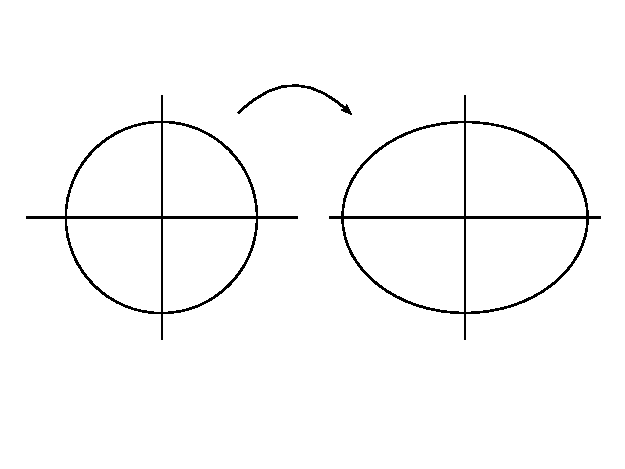
\includegraphics{img/15_screwing_map.pdf}
    \caption{How map $f$ might transform a circle}
  \end{center}
\end{figure}

\index{Eigenvalue}
\index{Eigenvector}
\index{Spectrum}
\begin{definition} % Definition 10.1
  $f \in \operatorname{Hom}(V, V) = \operatorname{End}(V)$.
  $\lambda \in \mathbb K$ is called \emph{eigenvalue} if
  $\exists v \in V \setminus \set{0}: f(v) = \lambda \cdot v$.
  Then $v$ is called \emph{eigenvector} of eigenvalue $\lambda$.
  $\operatorname{spec}(f) = \set{\text{eigenvalues of } f}$ is called \emph{spectrum of $f$}.
\end{definition}

In 1925 in quantum mechanisms, it was discovered that the spectrum of light is given as a linear map (spectrum in the mathematical sense).

\subsection{Eigenspace}

\index{Eigenspace}
\begin{lemma}
  For $\lambda \in \mathbb K$, $f \in \operatorname{End}(V)$.
  \[ \eta_{\lambda} = \setdef{v}{f(v) = \lambda \cdot v} \]
  is a subspace and is called eigenspace of $f$ for eigenvalue $\lambda$.
\end{lemma}
\begin{proof}
  \[  f(v) = \lambda \cdot v \iff f(v) - \lambda \cdot v = 0
      \iff (f - \lambda \cdot \operatorname{id}) (v) = 0
      \iff v \in \underbrace{\operatorname{ker}(f - \lambda \cdot \operatorname{id})}_{\text{subspace}}
  \]
\end{proof}

\begin{example} % Beispiel 10.3
  \begin{enumerate}
    \item $f = \mu \cdot \operatorname{id}$. $\operatorname{spec}(f) = \set{\mu}$. $f(v) = \mu \cdot v \forall v \in V$. $\eta_\mu = V$.
    \item Let $b_1, \dots, b_n$ be a basis of $V$. Let $\lambda_1, \dots, \lambda_n \in \mathbb K$.
      Then there exists a unique, linear map $f$ such that $f(b_i) = \lambda_i \cdot b_i$.
      Every $b_i$ is an eigenvector to eigenvalue $\lambda_i$.
      \[ \eta_{\lambda} = \mathcal L(\setdef{b_i}{\lambda_i = \lambda}) \]
      Assume $f(v) = \lambda \cdot v$.
      \begin{align*}
        v &= \alpha_1 \cdot b_1 + \dots + \alpha_n b_n \\
        f(v) &= \alpha_1 f(b_1) + \dots + \alpha_n f(b_n) \\
          &= \alpha_1 \lambda_1 b_1 + \dots + \alpha_n \lambda_n b_n \\
          &= \lambda(\alpha_1 b_1 + \dots + \alpha_n b_n) \\
        \hline
        \implies 0 &= \alpha_1(\lambda_1 - \lambda) b_1 + \dots + \alpha_n(\lambda_n - \lambda) \cdot b_n \\
        \text{linear indep.} \implies& \forall i: \alpha_i (\lambda_i - \lambda) = 0 \\
        \text{hence either } \alpha_i = 0 \text{ or } \lambda_i = \lambda
      \end{align*}
      \[ \implies \operatorname{spec}(f) = \set{\lambda_1, \dots, \lambda_n} \]
      \[ \Phi_B^B(f) = \begin{bmatrix} \lambda_1 & & 0 \\ & \ddots & \\ 0 & & \lambda_n \end{bmatrix} \]
    \item Let $V = C^{\infty}(\mathbb R)$.
      \[ \frac{d}{dx} y(x) = \lambda \cdot y(x) \qquad \frac{dy}{dx} = \lambda \cdot y \]
      \[ \int \frac{dy}{y} = \int \lambda \cdot dx \]
      \index{Eigen function}
      \[ \operatorname{log}(y) = \lambda \cdot x + C \qquad \text{ \emph{Eigen function} (compare with Fourier analysis)} \]
      \[ y = C \cdot e^{\lambda x} \]
      \[ \frac{d}{dx} e^{\lambda x} = \lambda \cdot e^{\lambda x} \]
    \item Let $V = C^{\infty}[0, a]$.
      \begin{align*}
        \frac{d^2}{dx^2} y(x) &= \lambda \cdot y(x) \\
        \frac{d^2}{dx^2} e^{\lambda x} &= \frac{d}{dx} \lambda e^{\lambda x} = \lambda^2 e^{\lambda x} \\
        \frac{d^2}{dx^2} e^{i \omega x} &= -\omega^2 e^{i\omega x} \\
        \frac{d^2}{dx^2} \sin{\omega x} &= \frac{d}{dx} \omega \cdot \cos(\omega x) = -\omega^2 \cdot \sin(\omega x) \\
        \frac{d^2}{dx^2} \cos{\omega \alpha} &= \frac{d}{dx} (-\omega) \sin(\omega x) = -\omega^2 \cos(\omega x)
      \end{align*}
      \[ y(0) = y_0 \to y(x) = y_0 \cdot e^{\lambda x} \]
      \[ y(0) = y(a) = 0 \]
      \[ y(x) = \sin(\omega x) \]
      \[ \omega a = k \cdot \pi \implies y(0) = y(a) = \pi \]
      \[ \omega = \frac{k \cdot \pi}{a} \]
      Eigenvalues of $H = P^2 + Q$ and $PQ - QP = \frac{\hbar}{i} I$. Heisenberg: Quantum mechanics is not commutative (impulses are matrices, not values).
  \end{enumerate}
\end{example}

\index{Right-sided eigenvalue}
\index{Left-sided eigenvalue}
\begin{definition} % Definition 10.4
  Let $A$ be a $n \times n$ matrix.
  $\lambda$ is called right-sided eigenvalue if $\exists x \in \mathbb K^n \setminus \set{0}: Ax = \lambda \cdot x$.
  $\lambda$ is called left-sided eigenvalue if $\exists x \in \mathbb K^n \setminus \set{0}: x^T A = \lambda \cdot x^T$
  But this definition is satisfied $\iff A^T x = \lambda \cdot x$, hence right-sided eigenvalue of $A^T$.
  Thus, these definitions collapse.
\end{definition}

\begin{lemma} % Lemma 10.5
  Left-sided eigenvalue $\iff$ right-sided eigenvalue.
\end{lemma}
\begin{proof}
  Let $\lambda$ be a right-sided eigenvalue.
  \begin{align*}
    Ax = \lambda x &\iff (A - \lambda \cdot I) \cdot x = 0 \\
      &\iff \exists x \neq 0: x \in \ker(A - \lambda I) \\
      &\iff \ker(A - \lambda I) \neq \set{0} \\
      &\iff \rank(A - \lambda I) < n \\
      &\iff \rank(A^T - \lambda I) < n \\
      &\iff \ker(A^T - \lambda I) \neq \set{0} \\
      &\iff \exists x \neq 0: A^T x = \lambda \cdot x \\
      &\iff \lambda \text{ is a left-sided } eigenvalue
  \end{align*}
\end{proof}

\begin{example} % Beispiel 10.6
  For $\dim = \infty$, this must not hold.
  \[ S: \begin{array}{c} \mathbb K^\infty \to \mathbb K^\infty \\ (x_1, x_2, \dots) \mapsto (x_2, x_3, \dots) \end{array} \]
  \[ S(1, 0, \dots) = (0, 0, \dots) \]
  \[ \implies (1, 0, \dots) \text{ is eigenvector for eigenvalue } 0 \]
  hence, element of $\ker(S)$.
  \[
    S = \begin{bmatrix}
      0 & 1 & 0 & 0 \\
      \vdots & 0 & 1 & 0 \\
      \vdots & \vdots & 0 & 1 \\
      \vdots & \vdots & \vdots & 0 \\
      \vdots & \vdots & \vdots & \vdots \\
      0 & & &
    \end{bmatrix}
  \] \[
    S^T = \begin{bmatrix}
      0 & & & \\
      1 & 0 &  & 0 \\
        & 1 & \ddots & \\
        & \ddots & \ddots & \\
      0 &  & 1 & 0
    \end{bmatrix}
  \]
  $S^T(x_1, x_2, \dots) \mapsto (0, x_1, x_2)$ is injective.
  $\ker(S^T) = \set{0}$. Hence $0$ is no eigenvalue.
  $0$ is right-sided eigenvalue of $S$, but not left-sided eigenvalue.
\end{example}

\begin{Remark}
  The theory of eigenvalues in infinite-dimensional spaces is more complex than the finite-dimensional case.
\end{Remark}

\begin{definition} % Definition 10.7
  For $A \in \mathbb K^{n \times n}$.
  \begin{align*}
    \operatorname{spec}(A) &= \set{\text{right-sided eigenvalue of } A} \\
        &= \set{\text{left-sided eigenvalue of } A}
  \end{align*}
  is called \emph{spectrum of $A$}.
\end{definition}

\begin{Remark}[Proof exercise]
  $\dim{V} = n, f \in \operatorname{End}(V), B$ is basis of $V$.
  \[ \implies \operatorname{spec}(f) = \operatorname{spec}(\Phi_B^B(f)) \]
\end{Remark}

\begin{Remark}
  Recall that any basis exchange can be done using some $T$:
  \[ \Phi_B^B(A) = T^{-1} A T \]
\end{Remark}

\begin{corollary}
  The spectrum does not depend on the choice of the basis. Hence,
  \[ \operatorname{spec}(T^{-1} AT) = \operatorname{spec}(A) \]

  \begin{proof}[Direct proof]
    Let $x$ be an eigenvector of $A$.
    \begin{align*}
      Ax = \lambda x &\iff A \cdot I \cdot x = \lambda x \iff A \cdot T \cdot T^{-1} \cdot x = \lambda x \\
                     &\iff T^{-1} \cdot A \cdot T \cdot T^{-1} \cdot x = T^{-1} \cdot \lambda x = \lambda \cdot T^{-1} \cdot x \\
                     &\iff y \coloneqq T^{-1} x \text{ is eigenvector of } T^{-1} AT \\
                     &\iff T^{-1} AT y = \lambda y \\
                     &\iff \lambda \text{ is eigenvalue of } T^{-1} AT
    \end{align*}
  \end{proof}
\end{corollary}

\begin{Remark}
  $\lambda$ is eigenvalue of $A$.
  \begin{align*}
    &\iff \ker(\lambda \cdot I - A) \neq \set{0} \\
    &\iff \rank(\lambda \cdot I - A) < n \\
    &\iff \det(\lambda \cdot I - A) = 0
  \end{align*}
\end{Remark}

\subsection{Characteristic polynomial}

\index{Characteristic polynomial}
\begin{theorem}[Theorem and definition] \hfill{} % Satz & Definition 10.10
  \begin{description}
    \item[Definition] $\chi_A(\lambda) \coloneqq \det(\lambda \cdot I - A)$ is a polynomial function and is called \emph{characteristic polynomial of $A$}.
    \item[Theorem] $\lambda$ is eigenvalue $\iff \chi_A(\lambda) = 0$
  \end{description}
\end{theorem}

\begin{example} % Beispiel 10.11
  \[
    A = \begin{bmatrix}
      -1 & 1 & 2 \\
      -1 & -5 & 2 \\
      2 & -2 & -4
    \end{bmatrix}
  \]
  \[
    \chi_A(\lambda) = \det(\lambda I - A)
    = \begin{vmatrix}
      \lambda + 1 & -1 & -2 \\
      1 & \lambda + 5 & -2 \\
      -2 & 2 & \lambda+4
    \end{vmatrix}
    = \begin{vmatrix}
      \lambda+1 & -1 & -2 \\
      1 & \lambda+5 & -2 \\
      0 & 2\lambda+12 & \lambda
    \end{vmatrix}
  \] \[
    = \begin{vmatrix}
      \lambda & -\lambda-6 & 0 \\
      1 & \lambda+5 & -2 \\
      0 & 2\lambda+12 & \lambda
    \end{vmatrix} = \lambda \cdot \begin{vmatrix}
      \lambda+5 & -2 \\
      2\lambda+12 & \lambda
    \end{vmatrix}
    - \begin{vmatrix}
      -\lambda - 6 & 0 \\
      2\lambda+12 & \lambda
    \end{vmatrix}
  \] \[
    = \lambda \cdot [\lambda^2 + 5\lambda + 4\lambda + 24] - \lambda(-\lambda-6)
  \] \[
    = \lambda(\lambda^2 + 5\lambda + 4\lambda + 24 + \lambda + 6)
  \] \[
    = \lambda(\lambda^2 + 10\lambda + 30)
  \] \[
    x_1 = 0 \qquad \lambda_{2,3} = \frac{-10 \pm \sqrt{10^2 - 120}}{2} = \frac{-10 \pm 2\sqrt{-5}}{2} = -5 \pm i\sqrt{5}
  \]
  Thus, the existence of eigenvalues depends on the field.
\end{example}

\begin{Remark}
  A square matrix $A$ is invertible if and only if $0$ is not an eigenvalue of $A$.
\end{Remark}

\subsection{Symmetrical minor}

\index{Symmetrical minors}
\begin{theorem} % Satz 10.12
  Let $A \in \mathbb K^{n \times n}$. Then $\chi_A(x) = \det(x \cdot I - A)$ is a polynomial of degree $n$.
  Specifically, $\chi_A(x) = \sum_{k=0}^n (-1)^{n-k} c_k(A) \cdot x^k$ with $c_k(A) \coloneqq \sum_{\substack{J \subseteq \set{1, \dots, n} \\ |J| = n - k}} \det(A_{JJ})$
  with $A_{JJ} \coloneqq (a_{ij})_{\substack{i \in J \\ j \in J}}$ are called \emph{symmetrical minors}.
\end{theorem}

\begin{Remark}
  What are special values of $c_i$?
  \[
    c_0 = \det(A) \qquad
    c_n = 1 \qquad
    c_{n-1} = \sum a_{ii} = \operatorname{Tr}(A)
  \]
\end{Remark}

\begin{proof}
  The proof is given using the Leibniz formula for determinants.
  \begin{align*}
    \det(x \cdot I - A) &= \sum_{\pi \in \sigma_n} (-1)^\pi \prod_{i=1}^n \underbrace{(x \cdot I - A)_{\pi(i),i}}_{x \cdot \delta_{\pi(i),i} - a_{\pi(i),i}} \\
      &= (x - a_{11})(x - a_{22}) \dots (x - a_{nn}) +
        \underbrace{
          \sum_{\substack{\pi \in \sigma_n \\ \pi \neq \operatorname{id}}}
          (-1)^\pi \prod_{i=1}^n
          \left(x \delta_{\pi(i),i} - a_{\pi(i),i}\right)
        }_{\text{for at least 2 $i$, $\delta_{\pi(i),i} = 0$}} \\
      &= \text{ expression of degree } n + \text{ expression of degree } n -2
  \end{align*}
  Hence $\det(x \cdot I - A)$ retains as expression of polynomial degree $n$. Hence the degree of $\chi_A(x)$ is $n$.
  \begin{align*}
    \det{\prod_{i=1}^n (x \delta_{\pi(i),i} - a_{\pi(i),i})} &= \#\setdef{i}{\pi(i) = i} \\
      &= \#\operatorname{fixedpoints}(\pi)
  \end{align*}
  Let $s_1, \dots, s_n$ be the columns of $A$.
  \[ \det(xI - A_i) = \triangle(x\cdot e_1 - s_1, x \cdot e_2 - s_2, \dots, x \cdot e_n - s_n) = \sum_{I \subseteq \set{1, \dots, n}} \triangle(y_1, \dots, y_n) \]

  \[ y_i = \begin{cases} x \cdot e_i & i \in I \\ -s_{i_k} & i \in I^C \end{cases} \]
  Let $k \in I$.
  \[
    \triangle(y_1, \dots, y_{k-1}, x \cdot e_k, y_{k+1}, \dots, y_n) = \begin{vmatrix}
      y_1 & y_2 & \dots & y_{k-1} & 0 & y_{k+1} & \dots & y_n \\
      \vdots & \vdots & \vdots & \vdots & \vdots & \vdots & \vdots & \vdots \\
      \vdots & \vdots & \vdots & \vdots & 0 & \vdots & \vdots & \vdots \\
      \vdots & \vdots & \vdots & \vdots & x & \vdots & \vdots & \vdots \\
      \vdots & \vdots & \vdots & \vdots & 0 & \vdots & \vdots & \vdots \\
      \vdots & \vdots & \vdots & \vdots & \vdots & \vdots & \vdots & \vdots \\
      \vdots & \vdots & \vdots & \vdots & 0 & \vdots & \vdots & \vdots
    \end{vmatrix}
  \]
  Permute the $k$-th column into the first column: $(-1)^{k-1}$. \\
  Permute the $k$-th row into the first row: $(-1)^{k-1}$.
  \[
    = \begin{vmatrix}
      x & \tilde{y_1} & \tilde{y_2} & \dots & \tilde{k-1} & \tilde{k+1} & \dots & \tilde{n} \\
      0 & \vdots & \vdots & \vdots & \vdots & \vdots & \vdots & \vdots \\
      \vdots & \vdots & \vdots & \vdots & \vdots & \vdots & \vdots & \vdots \\
      0 & \vdots & \vdots & \vdots & \vdots & \vdots & \vdots & \vdots \\
    \end{vmatrix}
    = x \cdot \begin{vmatrix}
      \tilde{\tilde{y_1}} & \dots & \tilde{\tilde{y_{k-1}}} & \tilde{\tilde{y_{k+1}}} & \vdots & \tilde{\tilde{y_n}} \\
      \vdots & \vdots & \vdots & \vdots & \vdots & \vdots
    \end{vmatrix}
  \]
  where $\tilde{y}$ is the permutation of $y_i$ such that the $k$-th row moved to the first.

  Every time, one $x$ is eliminated, the corresponding row and column of $A$ is removed.
  In the end,
  \[ x^{\card{I}} \cdot \underbrace{\det{A_{I^C I^C}}}_{\text{minor of the complement $\card{I^C} = n-k$}} \cdot (-1)^{\card{I^C}} \]
  \begin{align*}
    \implies \chi_A(x) &= \sum_{I \subseteq \set{1, \dots, n}} x^{\card{I}} \cdot \det[A_{I^C I^C}] (-1)^{\card{I^C}}
      &= \sum_{k=0}^n x^k (-1)^{n-k} c_k(A)
  \end{align*}
  with $c_k(A) = \sum_{\card{J} = n-k} \det[A_{jj}]$.
\end{proof}

\dateref{2018/05/16}

% Revision:
% \[ Ax = \lambda x \]
% \[ x \in \ker(\lambda \cdot I - A) \]
% \[ \chi_A(\lambda) = \det(\lambda I - A) = x^n - \operatorname{Tr}(A) x^{n-1} + \dots (-1)^n \det(A) \]
% Characteristic polynomial: $= \sum_{k=0}^n (-1)^{n-k} c_k x^k$
% \[ c_k = \sum_{\card{J} = n-k} \det[A_{J,J}] \]
% \[ T^{-1} AT \cdot T^{-1} x = \lambda T^{-1} x \]

\begin{lemma} % 10.13
  \[ \chi_{T^{-1} AT}(x) = \chi_A(x) \]
\end{lemma}
\begin{proof}
  \begin{align*}
    \chi_{T^{-1}AT}(x) &= \det(xI - T^{-1}AT) \\
      &= \det(x T^{-1} T - T^{-1} AT) \\
      &= \det(T^{-1} (x \cdot I) T - T^{-1} (A) T) \\
      &= \det(T^{-1}(x \cdot I - A) \cdot T) \\
      &= \det(T^{-1}) \cdot \det(xI - A) \cdot \det(T) \\
      &= \frac{1}{\det{T}} \cdot \chi_A(x) \cdot \det{T} = \chi_A(x)
  \end{align*}
\end{proof}

\[ A = \begin{pmatrix} a_{11} & & 0 \\ & \ddots & \\ 0 & & a_{nn} \end{pmatrix} \leadsto \operatorname{spec}(A) = \set{a_{11}, \dots, a_{nn}} \]
Eigenvector: $e_1, \dots, e_n$.

\begin{Remark}[Question]
  Does a change of basis exist, hence $T \in \operatorname{GL}(n)$, such that $T^{-1} AT = \operatorname{diag}(\lambda_1, \dots, \lambda_n)$?
  Then the eigenvalues are necessarily on the diagonal.
\end{Remark}

\subsection{Diagonalizable matrix}

\index{Diagonalizable matrix}
\begin{definition} % Definition 10.14
  $A$ is called \emph{diagonalizable} if $\exists T \in \operatorname{GL}(n)$ such that $T^{-1} \cdot AT$ is a diagonal matrix,
  i.e. $A$ is \emph{similar} to a diagonal matrix.
\end{definition}

\begin{Remark}[Recall]\hfill{}
  \begin{description}
    {\leftskip=15pt
    \item[Equivalence] $A = PBQ$ with invertible $P,Q \iff \rank(A) = \rank(B)$.
    \item[Congruence] $\exists \text{ invertible } C: A = C^* BC$ \\
      For $A = A^*, B = B^*$, $\leadsto$ index and Sylvester's law of inertia.
    \item[Similarity] $A = TBT^{-1}$ with invertible $T$. This is related to eigenvalues.
    \item[Later on] $\exists T$ such that $T^* = T^{-1}$ unitary. $T^{*} T = I$.

    }
  \end{description}
\end{Remark}

\begin{lemma} % Lemma 10.15
  $A$ is diagonalizable $\iff \exists$ basis of eigenvectors.
\end{lemma}

\begin{proof}
  $B$ is invertible such that
  \[
    B^{-1} AB = \begin{bmatrix} \lambda_1 & & \\ & \ddots & \\ & & \lambda_n \end{bmatrix}
    \iff \begin{cases}
      \exists \text{ columns } b_{1}, \dots, b_n \text{ define a basis} \\
      AB = B \begin{bmatrix} \lambda_1 & & \\ & \ddots & \\ & & \lambda_n \end{bmatrix} \\
      A \cdot \begin{bmatrix} b_1 & b_2 & \dots & b_n \\ \vdots & \vdots & \vdots & \vdots \end{bmatrix} = \begin{bmatrix} b_1 & b_2 & \dots & b_n \\ \vdots & \vdots & \vdots & \vdots \end{bmatrix} \cdot \begin{bmatrix} \lambda_1 &  & 0 \\ & \ddots & \\ 0 & & \lambda_n \end{bmatrix} \\
      \begin{bmatrix} Ab_1 & Ab_2 & \dots & Ab_n \\ \vdots & \vdots & \vdots & \vdots \end{bmatrix} = \begin{bmatrix} b_1 \lambda_1 & b_2 \lambda_2 & \dots & b_n \lambda_n \\ \vdots & \vdots & \vdots & \vdots \end{bmatrix}
    \end{cases}
  \] \[
    \iff \begin{cases}
      \exists \text{ basis } b_1, \dots, b_n \\
      A \cdot b_i = \lambda \cdot b_i \qquad i = 1, \dots, n
    \end{cases}
  \]
\end{proof}

\begin{example} % Beispiel 10.16
  \[ A = \begin{bmatrix} 1 & 2 & 4 \\ 4 & -3 & -8 \\ -2 & 2 & 5 \end{bmatrix} \]
  \begin{align*}
    \chi_A(\lambda) &= \det(\lambda I - A) = \begin{vmatrix}
      \lambda+1 & -2 & -4 \\
      -4 & \lambda+3 & 8 \\
      2 & -2 & \lambda-5
    \end{vmatrix}
    = \begin{vmatrix}
      \lambda-1 & -2 & -4 \\
      \lambda-1 & \lambda+3 & 8 \\
      0 & -2 & \lambda-5
    \end{vmatrix} \\
    &= (\lambda - 1) \begin{vmatrix} 1 & -2 & -4 \\ 1 & \lambda+3 & 8 \\ 0 & -2 & \lambda-5 \end{vmatrix}
    = (\lambda - 1) \begin{vmatrix} 1 & -2 & -4 \\ 0 & \lambda+5 & 12 \\ 0 & -2 & \lambda-5 \end{vmatrix} \\
    &= (\lambda-1)(\lambda^2 - 25 + 24) = (\lambda - 1)(\lambda^2 - 1) = (\lambda-1)^2 (\lambda + 1)
  \end{align*}
  Eigenvalue $(\lambda-1)$ has multiplicity $2$.

  Eigenvector: $\ker(\lambda \cdot I - A)$ \\
  Eigenvalue: $\lambda = \pm 1$

  Consider $\lambda = +1$: $\ker(I - A)$

  Homogeneous equation system:
  \[
    \begin{array}{ccc|c}
      2 & -2 & -4 & 0 \\
      -4 & 4 & 8 & 0 \\
      2 & -2 & -4 & 0 \\
    \hline
      0 & 0 & 0 & \\
      0 & 0 & 0 &
    \end{array}
  \]
  $\dim\ker(I - A) = 2$. $2x_1 = 2x_2 + 4x_3$.

  Basis:
  \[ \begin{pmatrix} 1 \\ 1 \\ 0 \end{pmatrix} \quad \begin{pmatrix} 2 \\ 0 \\ 1 \end{pmatrix} \]

  Consider $\lambda = -1$: $\ker(-I - A)$
  \[
    \begin{array}{ccc|c}
      0 & -2 & -4 & 0 \\
      -4 & 2 & 8 & 0 \\
      2 & -2 & -6 & 0 \\
    \hline
      0 & -2 & -4 \\
      0 & -2 & -4 \\
    \hline
      0 & 0 & 0
    \end{array}
  \]
  $\dim\ker(-I - A) = 1$.

  Basis:
  \begin{align*}
    x_3 &= 1 \\
    x_2 &= -2x_3 = -2 \\
    x_1 &= \frac{2x_2 + 6x_3}{2} = 1
  \end{align*}
  \[ b_3 = \begin{pmatrix} 1 \\ -2 \\ 1 \end{pmatrix} \]

  with $B = \begin{bmatrix} 1 & 2 & 1 \\ 1 & 0 & -2 \\ 0 & 1 & 1 \end{bmatrix}$
  it holds that $B^{-1} AB = \begin{bmatrix} 1 &  & \\ & 1 & \\ & & -1 \end{bmatrix}$.
\end{example}

\begin{Example}[Application]
  \begin{align*}
    A &= B^{-1} \cdot \underbrace{\begin{bmatrix} \Lambda_1 & & \\ & \ddots & \\ & & \Lambda_n \end{bmatrix}}_{\Lambda} \cdot B \\
    A^2 &= B^{-1} \Lambda B \cdot B^{-1} \Lambda B = B^{-1} \Lambda^2 B \\
    A^3 &= B^{-1} \Lambda^3 B \\
        & \vdots \\
    A^k &= B^{-1} \Lambda^k B
  \end{align*}
  \[ e^A = \sum_{k=0}^\infty \frac{A^k}{k!} = \sum_{k=0}^\infty \frac{B^{-1} \Lambda^k B}{k!} = B^{-1} \sum_{k=0}^\infty \frac{\Lambda^k}{k!} B = B^{-1} \begin{bmatrix} e^{\lambda_1} & & \\ & \ddots & \\ & & e^{\lambda_n} \end{bmatrix} \]
\end{Example}

\begin{Remark}
  Leondaro Pisano (1170--1250) wrote his book \enquote{Liber Abbaci} (1202) to introduce the Arabic numbers (and zero) in Europe.
  He also introduced the Fibonacci sequence using the growth of a rabbit population.
\end{Remark}

\subsection{Fibonacci sequence and golden ratio}

\begin{Remark}[Fibonacci sequence]
  \[ F_0 = F_1 = 1 \qquad F_n = F_{n-1} + F_{n-2} \]
  Can we find a formula for $F_n$?
\end{Remark}

\begin{Person}
  Pingala (200~BC)
\end{Person}

\begin{Remark}
  How many ways are there for the equation $x_1 + \dots + x_k = n$ for given $n$ and $x_i \ in \set{1,2}$?
  The answer is the Fibonacci sequence.

  His application was the number of long syllables (2) or short syllables (1) in a sentence of given length in Sanskrit.
\end{Remark}

\begin{Remark}[Growth of Fibonacci sequence]
  \[ F_{n+1} = F_n + F_{n-1} \qquad F_n = F_n \]
  \begin{align*}
    \vectwo{F_{n+1}}{F_n}
      = \vectwo{F_n + F_{n-1}}{F_n}
      &= \begin{bmatrix} 1 & 1 \\ 1 & 0 \end{bmatrix} \begin{bmatrix} F_n \\ F_{n-1} \end{bmatrix} 
      = \begin{bmatrix} 1 & 1 \\ 1 & 0 \end{bmatrix}^2 \begin{bmatrix} F_{n-1} \\ F_{n-2} \end{bmatrix} 
      = \begin{bmatrix} 1 & 1 \\ 1 & 0 \end{bmatrix}^3 \begin{bmatrix} F_{n-2} \\ F_{n-3} \end{bmatrix} \\
      &= \dots
      = \begin{bmatrix} 1 & 1 \\ 1 & 0 \end{bmatrix}^n \begin{bmatrix} F_1 \\ F_0 \end{bmatrix}
      = \begin{bmatrix} 1 & 1 \\ 1 & 0 \end{bmatrix}^n \vectwo11
  \end{align*}
  and where $\begin{pmatrix} 1 & 1 \\ 1 & 0 \end{pmatrix}$ is diagonalizable.
  \[
    \chi_A(\lambda) = \begin{vmatrix}
      \lambda-1 & -1 \\
      -1 & \lambda
    \end{vmatrix} = \lambda^2 - \lambda - 1
    \qquad
    \lambda_{1,2} = \frac{1 \pm \sqrt{1 + 4}}{2} = \frac{1 \pm \sqrt{5}}{2}
  \]

  \emph{Eigenvector:}
  Consider $\lambda_1 \coloneqq \frac{1 + \sqrt5}{2}$.
  \[
    \left(\begin{array}{cc|c}
      \frac{1 + \sqrt5}{2} - 1 & -1 & 0 \\
      -1 & \frac{1 + \sqrt5}{2} & 0
    \end{array}\right)
    \quad\implies\quad
    x_1 = \frac{1 + \sqrt5}{2} x_2 \qquad b_1 = \begin{bmatrix} \frac{1 + \sqrt5}{2} \\ 1 \end{bmatrix}
  \]
  Consider $\lambda_2 = \frac{1 - \sqrt5}{2}$.
  \[
    \left(\begin{array}{cc|c}
      \frac{1 - \sqrt5}{2} & -1 & 0 \\
      -1 & \frac{1 - \sqrt5}{2} & 0
    \end{array}\right)
    \quad\implies\quad
    x_1 = \frac{1 - \sqrt5}{2} x_2 \qquad
    b_2 = \begin{bmatrix} \frac{1 - \sqrt5}{2} \\ 1 \end{bmatrix} \]

  \[
    B = \begin{bmatrix} \frac{1 + \sqrt5}{2} & \frac{1 - \sqrt5}{2} \\ 1 & 1 \end{bmatrix} \qquad
    \det{B} = \frac{1 + \sqrt5}{2} - \frac{1 - \sqrt5}{2} = \sqrt5 \qquad
    B^{-1} = \frac{1}{\sqrt5} \begin{bmatrix} 1 & \frac{-1 + \sqrt5}{2} \\ -1 & \frac{1 + \sqrt5}{2} \end{bmatrix}
  \]
  \[
    \begin{bmatrix} a & b \\ c & d \end{bmatrix}^{-1} = \frac{1}{ad - bc} \begin{bmatrix} d & -b \\ -c & a \end{bmatrix} \qquad
    B^{-1} AB = \begin{bmatrix} \frac{1 + \sqrt5}{2} & 0 \\ 0 & \frac{1 - \sqrt5}{2} \end{bmatrix}
  \]
  \[ \vectwo{F_{n+1}}{F_n} = A^n \vectwo11 = B \begin{bmatrix} (\frac{1 + \sqrt5}{2})^n & \\ & (\frac{1 - \sqrt5}{2})^n \end{bmatrix} \cdot B^{-1} \cdot \begin{bmatrix} 1 \\ 1\end{bmatrix} \]
  \[ F_n = \frac1{\sqrt5} \left[\left(\frac{1 + \sqrt5}{2}\right)^{n+1} - \left(\frac{1 - \sqrt5}{2}\right)^{n+1}\right] \]

  \index{Golden ratio}
  \[ \frac{F_{n+1}}{F_n} = \frac{\left(\frac{1 + \sqrt5}{2}\right)^{n+2} - \left(\frac{1 - \sqrt5}{2}\right)^{n+1}}{\left(\frac{1 + \sqrt5}{2}\right)^{n+1} - \left(\frac{1 - \sqrt5}{2}\right)^{n+1}} \xrightarrow{n\to\infty} \frac{1 + \sqrt5}{2} \approx 1.6180 \]
  This limit is called \emph{Golden ratio}. It is the ratio:
  \[ \frac{a}{a+b} = \frac ba \qquad \frac{F_n}{F_{n-1}} = \frac{1}{1 + \frac{1}{1 + \frac{1}{\dots}}} \]
\end{Remark}

\begin{theorem} % Satz 10.18
  Eigenvectors corresponding to different eigenvalues are linear independent.
\end{theorem}

\begin{proof}
  Let $\lambda_1, \dots, \lambda_r$ be different eigenvalues of $A$. Let $v_1, \dots, v_r$ be their respective eigenvectors. Proof by induction over $r$.
  \begin{description}
    \item[Case $r=1$:]  immediate, $v_1 \neq 0$.
    \item[Case $r-1 \to r$:]
      Let $\alpha_1 v_1 + \dots + \alpha_r v_r = 0$.
      \[ \implies A \sum_{i=1}^r \alpha_i v_i = 0 \qquad
         \sum_{i=1}^r \alpha_i A v_i = 0 \qquad
         \sum_{i=1}^r \alpha_i \lambda_i v_i = 0 \]
  \end{description}

  \[ \begin{array}{rrl}
    (1): & \sum_{i=1}^{r} \alpha_i v_i &= 0 \\
    (2): & \sum_{i=1}^{r} \lambda_i \alpha_i v_i &= 0 \\
    \hline
    (2) - \lambda_r (1) \implies & \sum_{i=1}^{r} (\lambda_i - \lambda_r) \alpha_i v_i &= 0
  \end{array} \]
  By induction hypothesis: $v_1, \dots, v_{r-1}$ are linear independent.
  \begin{align*}
    \implies (\lambda_1 - \lambda_r) \alpha_1 &= 0 \\
    (\lambda_2 - \lambda_r) \alpha_2 &= 0 \\
    \vdots & \\
    (\lambda_{r-1} - \lambda_r) \alpha_{r-1} &= 0
  \end{align*}
  As all eigenvalues are different, $\lambda_i - \lambda_r \neq 0 \forall i < r$.
  \[ \implies \alpha_1 = \alpha_2 = \dots = \alpha_{r-1} = 0 \]
  \[ (1) \implies \alpha_r \cdot v_r = 0 \implies \alpha_r = 0 \text{ because } v_r \neq 0 \]
\end{proof}

\begin{corollary} % Folgerung 10.19
  An $n\times n$ matrix with $n$ different eigenvalues is diagonalizable.

  Hence, for every eigenvalue there exists some eigenvector. They are linear independent and $n$ elements.
  Hence they define a basis.
\end{corollary}

\begin{example} % Beispiel 10.20
  \[ A = \begin{bmatrix} 0 & 1 \\ 0 & 0 \end{bmatrix} \]
  \[ \chi_A(\lambda) = \begin{vmatrix} \lambda & -1 \\ 0 & \lambda \end{vmatrix} = \lambda^2 \]
  \[ \operatorname{spec}(A) = \set{0} \]
  \[ \dim\ker(A) = 1 \]
  is not a basis of eigenvectors.

  \[ A^2 = \begin{bmatrix} 0 & 1 \\ 0 & 0 \end{bmatrix}^2 = \begin{bmatrix} 0 & 0 \\ 0 & 0 \end{bmatrix} \]
  $A$ is nilpotent, hence a square matrix $M$ such that $M^k = 0$ for any $k \in \mathbb N_{\geq1}$.
\end{example}

\subsection{Multiplicities of eigenvalues}

\index{Geometric multiplicity of an eigenvalue}
\begin{definition} % Definition 10.21
  Let $\lambda$ be the eigenvalue of a matrix $A$ $\implies \chi_A(\lambda) = 0$. The
  \begin{description}
    \item[geometric multiplicity of $\mathbf\lambda$] is defined as $d(\lambda) \coloneqq \dim\ker(\lambda I - A) > 0$
    \item[algebraic multiplicity of $\mathbf\lambda$] is defined as, $k(\lambda)$, the multiplicity of $\lambda$ as root of $\chi_A(\lambda)$
  \end{description}
  \[ d(\lambda) \leq k(\lambda) \]
\end{definition}

\begin{lemma} % Lemma 10.22
  A matrix is diagonalizable iff for different eigenvalues $\lambda_1, \dots, \lambda_r$ it holds that
  \[ d(\lambda_1) + d(\lambda_2) + \dots + d(\lambda_r) = n \]
\end{lemma}

\begin{proof} \hfill{}
  \begin{description}
    \item[Direction $\implies$:]
      There exists a basis of eigenvectors $b_1, \dots, b_n$.
      \[ V = \eta_{\lambda_1} + \dots + \eta_{\lambda_r} \qquad \eta_{\lambda_i} = \ker(\lambda_i I - A) \]
      is a direct sum (because eigenvectors for different eigenvalues are linear independent).
      Let $v_1 \in \eta_{\lambda_1}, \dots, v_r \in \eta_{\lambda_r}$ such that $v_1 + \dots + v_r = 0$.
      \[ A v_i = \lambda_i v_i \implies v_1, \dots, v_r \text{ are linear independent } \implies \text{ all } v_i = 0 \]
      \[ \implies n = \dim{V} = \dim(\eta_{\lambda_1}) + \dots + \dim(\eta_{\lambda_r}) = d(\lambda_1) + \dots + d(\lambda_r) \]
    \item[Direction $\impliedby$.]
      Let $B_j$ be the basis of $\eta_{\lambda_j}$, hence $\card{B_j} = d(\lambda_j)$.
      The sum $\eta_{\lambda_1} + \dots + \eta_{\lambda_r}$ is direct.
      $\implies B_i \cup \dots \cup B_r$ is linear independent.
      \[ \card{B_1 \cup \dots \cup B_r} = \sum_{j=1}^r d(\lambda_j) \underbrace{=}_{\text{by induction}} \eta \]
      $B_i \cup \dots \cup B_n$ is basis of $\mathbb K^n$ of eigenvectors.
  \end{description}
\end{proof}

\begin{Remark}
  Why are there at most $n$ eigenvalues?

  We know the characteristic polynomial has degree $n$.

  For every eigenvalue, we have an algebraic multiplicity. Every algebraic multiplicity is at least 1.
  If there are more than $n$ eigenvalues, namely $n+1$, the sum of algebraic multiplicities of eigenvalues is at least $n+1$.
  Thus the degree of the characteristic polynomial (which is the sum of algebraic multiplicities of eigenvalues), is at least $n+1$ which contradicts our previous proof.
\end{Remark}

\begin{theorem} % Satz 10.23
  For every eigenvalue, it holds that
  \[ d(\lambda) \leq k(\lambda) \]
  Hence, the geometric multiplicity is smaller than the algebraic multiplicity.
\end{theorem}

\begin{proof}
  Let $\lambda \in \operatorname{spec}(A)$. Let $d = d(\lambda)$. Let $(b_1, \dots, b_d)$ be a basis of $\ker(\lambda I - A)$.
  We extend this vector to a basis of $\mathbb K^n:  (b_1, \dots, b_d, \dots, b_n)$.
  \[ B = \begin{pmatrix} b_1 & b_2 & \dots & b_n \\ \vdots & \vdots & \vdots & \vdots \end{pmatrix} \]
  \begin{align*}
    AB &= \begin{bmatrix} Ab_1 & Ab_2 & \dots & Ab_d & Ab_{d+1} & \dots & Ab_n \\ \vdots & \vdots & \vdots & \vdots & \vdots & \vdots & \vdots \end{bmatrix} \\
       &= \begin{bmatrix} \lambda b_1 & \lambda b_2 & \dots & \lambda b_d & Ab_{d+1} & \dots & Ab_n \\ \vdots & \vdots & \vdots & \vdots & \vdots & \vdots & \vdots \end{bmatrix} \\
	       &= \begin{bmatrix} b_1 & \dots & b_d & b & \dots & b_n \\ \vdots & \vdots & \vdots & \vdots & \vdots & \vdots \end{bmatrix} \begin{bmatrix} \lambda & & & \dots \\ & \lambda & & \dots \\ & & \lambda & \dots \\ 0 & 0 & 0 & \dots \\   & \dots 0 \dots &   & \dots \\ 0 & 0 & 0 & \dots \\ \end{bmatrix} \substack{\text{ where $\lambda$ occurs in} \\ \text{$d$ different columns}} \\
    B^{-1}AB &= \begin{bmatrix} \lambda & & & \dots \\ & \ddots & & \dots \\ & & \lambda & \dots \\ 0 & 0 & 0 & \\ 0 & 0 & 0 & \tilde A \\ 0 & 0 & 0 & \end{bmatrix} \eqqcolon M
  \end{align*}

  \begin{align*}
    \chi_A(x) &= \chi_{B^{-1} AB}(x) = \det(x \cdot I - M) \\
      &= \begin{bmatrix} x-\lambda & & & \dots \\ & \ddots & & \dots \\ & & x-\lambda & \dots \\ 0 & 0 & 0 & \\ 0 & 0 & 0 & xI_{n-d} - \tilde A \\ 0 & 0 & 0 & \end{bmatrix} \\
      &= (x - \lambda)^d \det(xI - \tilde A)
  \end{align*}
  $\implies x - \lambda$ is d-multiple factor of $\chi_A(x) \implies k(\lambda) \geq d(\lambda)$.
\end{proof}

\dateref{2018/05/23}

\begin{Remark}[Revision]
  $A$ is diagonalizable iff $\exists T$:
  \[ T^{-1} AT = \begin{bmatrix} \lambda_1 & & \\ & \ddots & \\ & & \lambda_n \end{bmatrix} \]
  where $T$ is basis of eigenvectors.
  \[ \iff d(\lambda) = \text{ geometric multiplicity } = \dim{\eta_{\lambda}} \]
  \[ \overset!= k(\lambda) = \text{ algebraic multiplicity} \]
\end{Remark}

\begin{Example}
  \[ A = \begin{bmatrix} \lambda & 1 & 0 \\ 0 & \lambda & 1 \\ 0 & 0 & \lambda \end{bmatrix} \]
  Eigenvalues:
  \[ \chi_A(x) = \begin{vmatrix} x - \lambda & -1 & 0 \\ 0 & x - \lambda & -1 \\ 0 & 0 & x - \lambda \end{vmatrix} = (x - \lambda)^3 \]
  The only eigenvalue: $\lambda$.
  $k(\lambda) = 3$.
  \[ \ker{\eta_{\lambda}} = \ker\begin{bmatrix} 0 & -1 & 0 \\ & 0 & -1 \\ & & 0 \end{bmatrix} \]
  \[ d(\lambda) = \dim\ker{\eta_{\lambda}} = 1 \implies \text{ not diagonalizable} \]
\end{Example}

\begin{Person}
  Camille Jordan (1838--1922): Jordan curve theorem.
\end{Person}

\section{Jordan Normal Form (JNF)} % Kapitel 11

\begin{Person}
  Causs-Wilhelm-Jordan (1842--1899)
\end{Person}

%% I think "Pasend Jordan" should mean "Pascual Jordan"
%% but the equation is still not correct for Jordan Algebras
%% https://en.wikipedia.org/wiki/Jordan_algebra
%Pasend Jordan Algebra: $A * B = A \cdot B + B \cdot A$

Nilpotent matrix:
\[
  \begin{bmatrix} 0 & * & * \\ 0 & 0 & * \\ 0 & 0 & 0 \end{bmatrix}^2
  = \begin{bmatrix} 0 & 0 & * \\ 0 & 0 & 0 \\ 0 & 0 & 0 \end{bmatrix}
  \qquad
  \begin{bmatrix} 0 & 0 & * \\ 0 & 0 & 0 \\ 0 & 0 & 0 \end{bmatrix}^2
  = \begin{bmatrix} 0 & 0 & 0 \\ 0 & 0 & 0 \\ 0 & 0 & 0 \end{bmatrix}
\]

\subsection{Invariant subspaces}

\index{Invariant subspace}
\begin{definition} % Definition 11
  Let $f: V \to V$ (or matrix $A \in \mathbb K^{n\times n}$) be linear.
  A subspace $U \subseteq V$ is called \emph{invariant} under $f$, if $f(U) \subseteq U$ (and accordingly $\forall x \in U: Ax \in U$)
\end{definition}

\begin{example} % Beispiel 11.2
  \begin{enumerate}
    \item $\set{0}$. $f(0) = 0 \in \set{0}$. $V$ is trivially invariant.
    \item $\ker{f}$. Let $x \in \ker{f} \implies f(x) = 0 \implies f(f(x)) = 0 \implies f(x) \in \ker{f}$. \\
      $\im{f}$ is invariant. $y \in \im{f} \implies f(y) \in \im{f}$.
    \item Eigenspaces are invariant.
      \[ f(x) = \lambda \cdot x \implies f(f(x)) = f(\lambda \cdot x) = \lambda \cdot f(x) \implies f(x) \in \eta_{\lambda} \]
    \item If $U$ are invariant with $\dim{U} = 1$, then $U = \mathcal L(x)$ with $x$ as eigenvector. \\
      If $x \in U \setminus \set{0}$ ($\implies U = \mathcal L(x)$), $f(x) \in U$. $\exists \lambda \cdot f(x) = \lambda \cdot x \implies x$ is eigenvector.
    \item $A = \begin{bmatrix} a_{11} & \dots & \dots & \dots \\ & a_{22} & \dots & \dots \\ & & \ddots & \dots \\ & & & a_{nn} \end{bmatrix}$.
      \[ A \cdot e_1 = a_{11} \cdot e_1 \implies e_1 \text{ is eigenvalue } \implies \mathcal L(e_1) \text{ is invariant} \]
      \[ A(\lambda_1 e_1 + \lambda_2 e_2) = \lambda_1 a_{11} e_1 + a_{12} \lambda_2 e_2 + a_{22} \lambda_2 e_2 \in \mathcal L(e_1, e_2) \implies \mathcal L(e_1, e_2) \text{ is invariant} \]
      \[ A \cdot e_k \in \mathcal L(e_1, \dots, e_k) \implies \forall k: \mathcal L(e_1, \dots, e_k) \text{ is invariant} \]
  \end{enumerate}
\end{example}

Numerically unstable:
\[
  \begin{bmatrix} \lambda & & \\ & \ddots & \\ & & \lambda \end{bmatrix}
  \text{ is diagonalizable.}
\qquad
  \begin{bmatrix} \lambda & & \varepsilon \\ & \ddots & \\ 0 & & \lambda \end{bmatrix}
  \text{ is not diagonalizable}
\]

\begin{theorem} % Satz 11.3
  \label{s113}
  Let $A \in \mathbb K^{n\times n}, V = \mathbb K^n$.
  \begin{enumerate}
    \item If $U \subseteq V$ is invariant under $A$ and $p(x) \in \mathbb K[x]$, then $U$ is invariant under $p(A)$.
      \[
        p(x) \coloneqq \sum_{k=0}^n a_k x^k 
        \qquad p(A) = \sum_{k=0}^n a_k A^k
        \qquad \psi_A: \substack{\mathbb K[x] \to \mathbb K^{n\times n} \\ x \mapsto A}
      \]
    \item $U_1, \dots, U_k$ are invariant subspaces.
      \[ \implies U_1 \cap \dots \cap U_k, U_1 + \dots + U_k \text{ are invariant with respect to } A \]
  \end{enumerate}
\end{theorem}

\begin{proof}
  \begin{enumerate}
    \item Let $x \in U$.
      \[ \implies Ax \in U \qquad A^2 \cdot x = A \cdot \underbrace{(Ax)}_{\in U} \in U \quad \dots \quad A^k x \in U \implies \sum a_k A^k x \in U \]
      because it is a linear combination of elements of $U$ where $U$ is the subspace with $A^k x \in U$.
    \item Let $x \in \bigcap_{i=1}^k U_i$. $\implies \forall i: x \in U_i \implies \forall i: Ax \in U_i \implies Ax \in \bigcap_{i=1}^k U_i$.
      Let $x \in U_1 + \dots + U_k \implies x = u_1 + u_2 + \dots + u_k \text{ for } u_i \in U_i$.
      \[ \implies Ax = (\underbrace{Au_1}_{\in U_1} + \underbrace{Au_2}_{\in U_2} + \dots + \underbrace{Au_k}_{\in U_k}) \in U_1 + \dots + U_k \]
      \[ \implies U_1 + \dots + U_k \text{ is invariant} \]
  \end{enumerate}
\end{proof}

\begin{lemma} % Lemma 11.4
  Let $f: V \to V$ and $U \subseteq V$ be an invariant subspace.
  $\implies f|_U: U \to U$ is a homomorphism.
  (If $U$ is not invariant, $\varphi|_U: U \to V$ must not map $U \to U$.)
\end{lemma}

\begin{theorem} % Satz 11.5
  Let $f: V \to V$. Let $U, W \subseteq V$ be invariant with $V = U \dot+ W$.
  Let $B = \set{b_1, \dots, b_m}$ be a basis of $U$, $B' = \set{b_1', \dots, b_n'}$ is basis of $W$.
  $\implies B \cup B'$ is basis of $V$.
  \[
    \Phi_{B\cup B'}^{B\cup B'}(f) = \left[\begin{array}{c|c}
      \Phi_B^B(f|_U) & 0 \\
    \hline
      0 & \Phi_{B'}^{B'}(f|_W)
    \end{array}\right]
  \]
\end{theorem}

\begin{proof}[Proof of Theorem~\ref{s113}]\hfill{}
  In the first $m$ columns, we have the images of $b_i$ (basis of $U$)
  \[ U \text{ invariant } \implies f(b_i) \in U \]
  \[ \implies \text{ coordinates in regards of } b'_1 \dots b'_n \text{ are } 0 \]
  \[
    \begin{bmatrix}
      f(b_1) & \dots  & f(b_m) & f(b_1') & \dots  & f(b_m') \\
             & \ddots &        & 0       &        & 0 \\
             &        &        & 0       &        & 0 \\
      0      & \dots  & 0      & \ddots  &        & \\
      0      & \dots  & 0      &         & \ddots & \\
      0      & \dots  & 0      &         &        & \ddots \\
    \end{bmatrix}
  \]

  In the last $n$ columns, we can find the images of $b_j'$.
  $W$ is invariant $\implies f(b'_j) \in W \implies$ coordinate in regards of $b_1, \dots, b_m$ are $0$.
\end{proof}

\begin{corollary} % Korollar 11.6
  \label{k116}
  Let $f: V \to V$. $U_1, \dots, U_k \subseteq V$ is invariant with $V = U_1 \dot+ U_2 \dot+ \dots \dot+ U_k$.
  Let $B_i$ be basis of $U_i \implies B = B_1 \cup \dots \cup B_k$ is basis of $V$ and
  \[
    \Phi_B^B(f) = \left[\begin{array}{c|ccc}
      \Phi_{B_1}^{B_1}(f|_{U_1}) & 0 & 0 & 0 \\
    \hline
      0 & \Phi_{B_2}^{B_2}(f|_{U_2}) & 0 & 0 \\
      0 & \vdots & \ddots & 0 \\
      0 &   &  & \Phi_{B_k}^{B_k}(f|_{U_k})
    \end{array}\right]
  \]
  Hence, if $V$ can be decomposed into a direct sum of invariant subspaces, then $A$ can be transformed into block diagonal form.
  ($A$ is diagonalizable $\iff V$ can be decomposed into direct sum of one-dimensional subspaces)
\end{corollary}

\begin{corollary} % Korollar 11.7
  Corollary related to Corollary~\ref{k116}.
  \[ \chi_f(x) = \prod_{i=1}^k \chi_{f|_{U_i}}(x) \]
\end{corollary}

\subsection{Fitting lemma}

\begin{Person}
  Hans Fitting (1906--1938)
\end{Person}

\begin{lemma}[Fitting lemma]
  Let $\dim{V} = n, f \in \operatorname{End}(V)$.
  \begin{enumerate}
    \item $\set{0} \subseteq \ker{f} \subseteq \ker{f^2} \subseteq \ker{f^3} \subseteq \dots$ \\
          $\im{f} \supseteq \im{f^2} \supseteq \im{f^3} \supseteq \dots$
    \item $\exists m \leq n: \ker{f^m} = \ker{f^{m+1}}$
    \item The following statements are equivalent:
      \begin{enumerate}
        \item $\ker{f^m} = \ker{f^{m+1}}$
        \item $\im{f^m} = \im{f^{m+1}}$
        \item $\ker{f^m} = \ker{f^{m+k}} \forall k \geq 1$
        \item $\im{f^m} = \im{f^{m+k}} \forall k \geq 1$
        \item $\ker{f^m} \cap \im{f^m} = \set{0}$
        \item $V = \ker{f^m} \dot{+} \im{f^m}$
      \end{enumerate}
  \end{enumerate}
\end{lemma}

\begin{proof}
  \begin{enumerate}
    \item Let $x \in \ker{f}$. Then $f^2(x) = f(f(x)) = f(0) = 0$. \\
      Let $y \in \im{f^2}$. Then $\exists x: y = f(f(x))$. Thus $f(x) \in \im{f}$.
    \item If $\set{0} \subsetneq \ker{f} \subsetneq \ker{f^2} \subsetneq \dots \subsetneq \ker(f^m)$
      \[ \implies 0 < \dim{\ker{f}} < \dim{\ker{f^2}} < \dots < \dim{\ker{f^m}} \qquad
         \implies m \leq n \]
    \item We prove a set of equivalences.
      \begin{itemize}
        \item 
          We prove (a) $\iff$ (b).
          Because of (1.), we know
          \begin{align*}
            &\quad \ker(f^m) \subseteq \ker(f^{m+1}) \\
            \implies \ker(f^m) &= \ker(f^{m+1}) \\
            \iff \dim\ker{f^m} &= \dim\ker{f^{m+1}} \\
            \iff n - \dim\im(f^m) &= n - \dim\im(f^{m+1}) \\
            \iff \dim\im(f^m) &= \dim\im(f^{m+1}) \\
          \intertext{Because of (1.), $\im{f^m} \supseteq f^{m+1}$}
            \iff \im(f^m) &= \im(f^{m+1})
          \end{align*}
        \item
          The proof of (c) $\iff$ (d) follows analogously.
          The proofs (a) $\iff$ (c) and (d) $\iff$ (b) are trivial.
        \item
          We prove (a) $\iff$ (c):
          \[ 0 \subseteq \ker{f} \subseteq \ker{f^2} \subseteq \ker{f^3} \subseteq \dots \]
          \[ m_0 = \min\setdef{m}{\ker(f^m) = \ker(f^{m+1})} \]
          \begin{claim}
            \[ \ker{f^{m_0 + k}} = \ker{f^{m_0 + k + 1}} \forall k \geq 0 \]
          \end{claim}
          \begin{description}
            \item[Direction $\subseteq$:] Immediate.
            \item[Direction $\supseteq$:]
              Let $x \in \ker{f^{m_0 + k + 1}} \implies f^{m_0 + k + 1}(x) = f^{m_0 + 1}(f^k(x)) = 0$.
              \[ \implies f^k(x) \in \ker{f^{m_0 + 1}} = \ker{f^{m_0}} \implies f^{m_0 + k}(x) = 0 \implies x \in \ker{f^{m_0 + k}} \]
              with $f^k(x) \in \ker{f^{m_0 + 1}} = \ker{f^{m_0}}$ by the definition of $m_0$.
          \end{description}
        \item
          We prove (b) $\iff$ (d).
          Let $m_0 = \min\setdef{m}{\im{f^m} = \im{f^{m+1}}}$.
          \begin{claim} $\im{f^{m_0 + k}} = \im{f^{m_0 + k + 1}} \forall k \geq 0$. \end{claim}
          \begin{description}
            \item[Direction $\supseteq$:] Trivial.
            \item[Direction $\subseteq$:]
              Let $y \in \im{f^{m_0 + k}}$.
              \[ \implies \exists x: y = f^{m_0 + k}(x) = f^k(f^{m_0}(x)) \text{ with } f^{m_0}(x) \in \im{f^{m_0} = \im{f^{m_0 + 1}}} \]
              hence $\exists z: f^{m_0}(x) = f^{m_0 + 1}(z)$.
              \[ \implies y = f^k(f^{m_0 + 1}(z)) = f^{m_0 + k + 1}(z) \in \im{f^{m_0 + k + 1}} \]
          \end{description}
        \item We prove $\set{(a), (b), (c), (d)} \iff$ (e).
          Let $W = \im{f^m}$ be invariant under $f^m$.
          \[ g \coloneqq f^m|_W \in \operatorname{Hom(W, W)} \]
          \[ \ker{g} = \ker(f^m) \cap W = \ker{f^m} \cap \im{f^m} \]
          \[ \ker{f^m} \cap \im{f^m} = \set{0} \iff \ker{g} = \set{0} \]
          \[ \iff g \text{ linear} \land g \text{ injective } \land g \text{ surjective } \iff \im{g} = W \]
          \[ \iff f^m(f^m(V)) = f^m(V) \iff f^{2m}(W) = f^m(W) \]
          \[ f^{m+m}(v) = f^m(v) \]
          \[ \im{f^{m+m}} = \im{f^m} \]
          This is equivalent to statements 1 and 3, thus rendering our assumption $\ker{f^m} \cap \im{f^m} = \set{0}$ valid.
        \item We prove (d) $\iff$ (b).
          \[ \im{f^{m+m}} = \im{f^m} \iff \im{f^{m+1}} = \im{f^m} \]
        \item (f) $\implies$ (e) is trivial.
        \item We prove (e) $\impliedby$ (f).
          \[
            \left.\begin{array}{c}
              \dim\im{f^m} + \dim\ker{f^m} = n \\
              \im{f^m} \cap \ker{f^m} = \set{0}
            \end{array}\right\}
            \implies \im{f^m} \dot{+} \ker{f^m} = V
          \]
          because of dimensionality reasons.
      \end{itemize}
  \end{enumerate}
\end{proof}

\begin{Remark}
  The intersection of image and kernel of a linear map is only $\set{0}$.
\end{Remark}

\dateref{2018/05/28}

Fitting Lemma:
\[ \ker{A} \subseteq \ker{A^2} \subseteq \dots \subseteq \ker{A^r} \]
\[ \im{A} \supseteq \im{A^2} \supseteq \dots \supseteq \im{A^r} = \im{A^{r+1}} \]
\[ \ker{A^r} \oplus \im{A^r} = V \]
\[ \ker{A^r} \cap \im{A^r} = \set{0} \]

\begin{example} % Beispiel 11.9
  \[ A = \begin{bmatrix} 0 & 1 & \\ & 0 & 1 \\ & &  0 \end{bmatrix}
     \qquad \ker{A} = \mathcal L\vecthree 100
     \qquad \im{A} = \mathcal L\left(\vecthree 100, \vecthree 010\right) \]
  \[ A^2 = \begin{bmatrix} 0 & 0 & 1 \\ & 0 & 0 \\ & &  0 \end{bmatrix}
     \qquad \ker{A^2} = \mathcal L\left(\vecthree 100, \vecthree 010\right)
     \qquad \im{A^2} = \mathcal L\left(\vecthree 100\right) \]
  \[ A^3 = \begin{bmatrix} 0 & 0 & 0 \\ & 0 & 0 \\ & &  0 \end{bmatrix}
     \qquad \ker{A^3} = \mathbb K^3
     \qquad \im{A^3} = \set{0} \]

  \begin{mdframed}
    \[ x \in \ker{A^k} \implies A \cdot x \in \ker{A^{k-1}} \]
  \end{mdframed}
\end{example}

\begin{Example}
  \[
    A = \begin{bmatrix} \lambda & 1 &  \\ & \lambda & 1 \\ & & \lambda \end{bmatrix}
    \qquad \text{ eigenvalue: } \lambda
    \qquad \lambda I - A = \begin{bmatrix} 0 & -1 & \\ & 0 & -1 \\ & & 0 \end{bmatrix}
  \]
  \[
    \ker(\lambda I - A) = \mathcal L\left(\vecthree 100\right)
    \qquad \ker((\lambda I - A)^2) = \mathcal L\left(\vecthree 100, \vecthree 010\right)
  \]
  \begin{align*}
    x \in \ker((\lambda I - A)^2)
      &\implies (\lambda I - A) x \in \ker(\lambda I - A) \\
      &\implies Ax = \lambda x + b \qquad b \in \ker(\lambda I - A)
  \end{align*}
\end{Example}

\subsection{Generalized space}

\index{Generalized space}
\index{Generalized eigenvectors}
\begin{definition} % Definition 11.10
  Let $A \in \mathbb K^{n\times n}$, $\lambda \in \operatorname{spec}(A)$.
  Then $\ker(\lambda I - A)^n$ is called \emph{generalized space} (dt. \foreignlanguage{german}{Hauptraum})
  of $A$ for eigenvalue $\lambda$. The elements are called \emph{generalized eigenvectors}.

  Actually, $\ker(\lambda I - A)^n = \ker(\lambda I - A)^r$ and a generalized eigenvector satisfies
  \[ A \cdot x = \lambda \cdot x + y \qquad y \in \ker(\lambda I - A)^{r-1} \]
  with $r$ as first index such that $\ker(\lambda I - A)^r = \ker(\lambda I - A)^{r+1}$.
\end{definition}

Fitting:
\[ \mathbb K^n = \ker(\lambda I - A)^r \oplus \im(\lambda I - A)^r \]
Next step: decomposition for \emph{different} eigenvalues.

\begin{lemma} % Lemma 11.11
  \label{lemma1111}
  Let $\lambda_1, \dots, \lambda_k$ be different eigenvalues of $A$ and
  $\ker(\lambda I - A)^{r_i}$ the corresponding generalized spaces where
  \[ \ker(\lambda_i I - A)^{r_{i-1}} \subsetneq \ker(\lambda_i I - A)^{r_i} = \ker(\lambda_i \cdot I - A)^{r_i + 1} \]
  \[ \implies \bigcap_{i=1}^k \im(\lambda_i - A)^{r_i} \cap \ker((\lambda_1 I - A)^{r_1} (\lambda_2 I - A)^{r_2} \dots (\lambda_k I - A)^{r_k}) = \set{0} \]
\end{lemma}

\begin{Remark}
  \[ \ker(\lambda_1 I - A)^{r_1} \dots (\lambda_k I - A)^{r_k} \supseteq \ker(\lambda_i I - A)^{r_i} \forall i \]
  \[ \supseteq \ker(\lambda_1 I - A)^{r_1} + \dots + \ker(\lambda_k I - A)^{r_k} \]
  if $(\lambda_i I - A)^{r_i} \cdot x = 0$,
  \[ (\lambda_1 I - A)^{r_1} \dots (\lambda_k I - A)^{r_k} \cdot x \]
  \[ = (\lambda_1 I - A)^{r_1} \dots (\lambda_{i-1} I - A)^{r_{i-1}} (\lambda_{i+1} I - A)^{r+1} \dots (\lambda_k I - A)^{r_k} \cdot \underbrace{(\lambda_i \cdot I - A)^{r_i}}_{=0} x = 0 \]
  If one of the factors is zero, the product is zero.
  \[ p(A) \cdot q(A) = q(A) \cdot p(A) \text{ for arbitrary polynomials } p(x) \text{ and } q(x) \]
  especially: $p_i(x) = (\lambda_i - x)^{r_i}$. [I think this can be derived from Lemma~\ref{lemma95}~(1)]
\end{Remark}

\begin{example} % Example 11.12
  \[
    A = \begin{bmatrix}
      1 & 1 &   &   &   &   &   & \\
        & 1 &   &   &   &   &   & \\
        &   & 1 &   &   &   &   & \\
        &   &   & 2 & 1 & 0 &   & \\
        &   &   &   & 2 & 1 &   & \\
        &   &   &   &   & 2 &   & \\
        &   &   &   &   &   & 0 & -1 \\
        &   &   &   &   &   & 1 & 0
    \end{bmatrix}
    \text{ over $\mathbb R$}
  \]
  \[ \operatorname{spec}(A) = \set{1,2} \cup \underbrace{(\set{\pm i})}_{\not\in \mathbb R} \]

  Consider $\lambda = 1$.
  \[
    \ker\left( I - A \right) =
    \ker\begin{bmatrix}
      0 & -1 &   &    &    &    &    & \\
        & 0  &   &    &    &    &    & \\
        &    & 0 &    &    &    &    & \\
        &    &   & -1 & -1 &    &    & \\
        &    &   &    & -1 & -1 &    & \\
        &    &   &    &    & -1 &    & \\
        &    &   &    &    &    & 1  & 1 \\
        &    &   &    &    &    & -1 & 1
    \end{bmatrix}
  \]
  \[ \ker(I - A) = \mathcal L(e_1, e_2) \qquad \text{ the two zero columns} \]
  \[
    \ker(I - A)^2 = \ker\begin{bmatrix}
      0 & 0  &   &    &    &    &    & \\
      0 & 0  &   &    &    &    &    & \\
        &    & 0 &    &    &    &    & \\
        &    &   & -1 & -1 &    &    & \\ % )^2
        &    &   &    & -1 & -1 &    & \\ % )
        &    &   &    &    & -1 &    & \\ % )   is invertible
        &    &   &    &    &    & 1  & 1 \\ %  )^2
        &    &   &    &    &    & -1 & 1    %  )   is invertible
    \end{bmatrix}
  \]
  \[ \ker(I - A)^2 = \mathcal L(e_1, e_2, e_3) \]
  \[ \im(I - A)^2 = \mathcal L(e_4, e_5, e_6, e_7, e_8) \]
  Consider $\lambda = 2$.
  \[
    \ker(2I - A) = \ker\begin{bmatrix}
      1 & -1 &   &    &    &    &    & \\
        & 1  &   &    &    &    &    & \\
        &    & 1 &    &    &    &    & \\
        &    &   & 0  & -1 &    &    & \\
        &    &   &    & 0  & -1 &    & \\
        &    &   &    &    & 0  &    & \\
        &    &   &    &    &    & 2  & 1 \\
        &    &   &    &    &    & -1 & 2
    \end{bmatrix}
  \] \[
    \ker(2I - A) = \mathcal L(e_{4})
  \] \[
    \ker(2I - A)^2 = \ker\begin{bmatrix}
      1 & 1  &   &    &    &    &     \\   % }^2
        & 1  &   &    &    &    &     \\   % }   is invertible
        &    & 1 &    &    &    &     \\
        &    &   & 0  & 0  & 1  &     \\
        &    &   &    & 0  & 0  &     \\
        &    &   &    &    & 0  &     \\
        &    &   &    &    &    & [\text{invertible}]
    \end{bmatrix}
  \] \[
    \ker(2I - A)^2 = \mathcal L(e_4, e_5)
  \] \[
    \ker(2I - A)^3 = \mathcal L(e_4, e_5, e_6)
  \] \[
    \ker(2I - A)^3 = \mathcal L(e_1, e_2, e_3, e_7, e_8)
  \] \[
    \bigcap_{i=1}^2 \im(\lambda_i I - A)^{r_i} = \mathcal L(e_1, e_2, e_3, e_7, e_8) \cap \mathcal L(e_4, e_5, e_6, e_7, e_8) = \mathcal L(e_7, e_8)
  \]
  \begin{align*}
    (I - A)^2 \cdot (2I - A)^3 &= \begin{bmatrix}
      0 & 0 &   & & \\
      0 & 0 &   & & \\
        &   & 0 & & \\
        &   &   & [\text{invertible } 3 \times 3] & \\
        &   &   &       & [\text{invertible } 2 \times 2]
    \end{bmatrix} \\ &\cdot \begin{bmatrix}
      [\text{invertible } 2 \times 2] & & & & & \\
        & 1 &   &   &   & \\
        &   & 0 & 0 & 0 & \\
        &   & 0 & 0 & 0 & \\
        &   & 0 & 0 & 0 & \\
        &   &   &   &   & [\text{invertible } 2 \times 2]
    \end{bmatrix} \\ &= \begin{bmatrix}
      0 & 0 &   &   &   &   & \\
      0 & 0 &   &   &   &   & \\
        &   & 0 &   &   &   & \\
        &   &   & 0 & 0 & 0 & \\
        &   &   & 0 & 0 & 0 & \\
        &   &   & 0 & 0 & 0 & \\
        &   &   &   &   &   & [\text{invertible } 2\times 2]
    \end{bmatrix}
  \end{align*} \[
    \ker{(I - A)^2 \cdot (2I - A)^3} = \mathcal L(e_1, \dots, e_6) = \left(\bigcap (\lambda_i I - A)^{r_i}\right)^c
  \]
\end{example}

\begin{Remark}
  Let $f$ and $g$ be matrices. Let $A$ and $B$ be corresponding linear maps.
  Then $A \cdot B$ is the matrix corresponding to $f \circ g$.
\end{Remark}

\begin{proof}[Proof of Lemma~\ref{lemma1111}]
  Show: If $x \in \bigcap{i=1}^k \im(\lambda_i I - A)^{r_i}$ and $(\lambda_1 I - A)^{r_1} \dots (\lambda_k I - A)^{r_k} \cdot x = 0$, then $x = 0$.

  Proof by induction over $k$:
  \begin{description}
    \item[Case $k=1$]
      \[ x \in \im(\lambda_1 I - A)^{r_1} \land (\lambda_1 I - A)^{r_1} x = 0 \]
      \[ \xRightarrow{\text{Fitting}} x = 0 \]
    \item[Case $k \to k+1$]
      Let $x \in \bigcap_{i=1}^k \im(\lambda_i I - A)^{r_i}$ and $(\lambda_1 I - A)^{r_1} \dots (\lambda_{k+1} I - A)^{r_{k+1}} x = 0$.
      Let $y = (\lambda_{k+1} - A)^{r_{k+1}} x \implies y \in \ker(\lambda_i I - A)^{r_i} \dots (\lambda_k I - A)^{r_k}$.
      \begin{align*}
        \forall i \in \set{1, \dots, k+1} \exists u_i: x &= (\lambda_i I - A)^{r_i} \cdot u_i \\
        y = (\lambda_{k+1} - A)^{r_{k+1}} x &= (\lambda_{k+1} - A)^{r_{k+1}} (\lambda_i I - A)^{r_i} \cdot u_i \\
          &= (\lambda_i I - A)^{r_i} (\lambda_{k+1} I - A)^{r_{k+1}} u_i \\
          &\in \im(\lambda_i I - A)^{r_i}
      \end{align*}
      \[ p(A) q(A) = q(A) p(A) \]
      \[ p(x) = (\lambda_{k+1} - x)^{r_{k+1}} \qquad q(x) = (\lambda_i - x)^{r_i} \]
      \[ \implies y \in \bigcap_{i=1}^{k} \im(\lambda_i I - A)^{r_i} \]
      By the induction hypothesis, $y = 0$.
      \[ \implies x \in \ker(\lambda_{k+1} I - A)^{r_{k+1}} \land x \in \im(\lambda_{k+1} I - A)^{r_{k+1}} \]
      \[ \xRightarrow{\text{Fitting}} x = 0 \]
  \end{description}
\end{proof}

\begin{lemma} \hfill{} % Lemma 11.13
  \label{le1113}%
  \begin{enumerate}
    \item $\forall \lambda \neq \mu \in \operatorname{spec}(A) \forall k,l \geq 1: \ker(\lambda I - A)^k \cap \ker(\mu I - A)^l = \set{0}$
    \item The sum $\sum_{i=1}^k \ker(\lambda_i I - A)^{r_i}$ is direct for arbitrary pairwise different $\lambda_1, \dots, \lambda_k$.
  \end{enumerate}
\end{lemma}

\begin{proof}
  Proof of the first statement. Induction over $m = k + l$.
  \begin{description}
    \item[Induction base] 
      Consider $m = 2, k = l = 1$.
      \[ \ker(\lambda I - A) \cap \ker(\mu I - A) = \set{0} \]
      The eigenvectors for different eigenvalues are linear independent.
    \item[Induction step $m-1 \to m$:]
      Consider $m \geq 3$. Without loss of generality: $k \geq 2$.
      Let $x \in \ker(\lambda I - A)^k \cap \ker(\mu I - A)^l$.
      Let $y = (\lambda I - A)x \in \ker(\lambda I - A)^{k-1} \cap \ker(\mu I - A)^l$. Then,
      \[ (\mu I - A)^l \cdot y = (\mu I - A)^l (\lambda I - A) \cdot x = (\lambda I - A) \underbrace{(\mu I - A)^l \cdot x}_{=0} = 0 \]
      Let $k - 1 + l = m - 1$.
      By induction hypothesis, $y = 0$.
      \[ \implies x \in \ker(\lambda I - A) \]
      \[ \implies x \in \ker(\lambda I - A) \cap \ker(\mu I - A)^l \xRightarrow{\text{induction hypothesis}} x = 0 \]
      \[ 1 + l \leq m - 1 \]
  \end{description}

  Proof of the second statement. Induction over $k$.
  \begin{description}
    \item[Induction base $k = 1$:] trivial
    \item[Induction step $k \to k+1$] \hfill{} \\
      Show: if $v_i \in \ker(\lambda_i I - A)^{r_i} \quad i = 1, \dots, k+1$ and $v_1 + \dots + v_{k+1} = 0
      \implies \text{ all } v_i = 0$.

      Let $w_i = (\lambda_{k+1} I - A)^{r_{k+1}} v_i \implies w_{k+1} = 0$.
      \[ \sum_{i=1}^k w_i = \sum_{i=1}^{k+1} w_i = (\lambda_{k+1} I - A)^{r_{k+1}} \underbrace{\sum_{i=1}^{k+1} v_i}_{=0} = 0 \]

      \[ (\lambda_i - A)^{r_i} w_i = (\lambda_i I - A)^{r_i} (\lambda_{k+1} I - A)^{r_{k+1}} v_i = (\lambda_{k+1} I - A)^{r_{k+1}} \underbrace{(\lambda_i I - A)^{r_i} \cdot v_i}_{=0} = 0 \]
      \[ p(x) = (\lambda_i - x)^{r_i} \qquad q(x) = (\lambda_{k+1} - x)^{r_{k+1}} \]
      \[ \implies w_i \in \ker(\lambda_i I - A)^{r_i} \]
      \[ \xRightarrow{\text{induction hypothesis}} w_i = 0 \forall i \]
      \[ \implies v_i \in \ker(\lambda_{k+1} I - A)^{r_{k+1}} \]
      \[ v_i \in \ker(\lambda_i I - A)^{r_i} \]
      \[ \implies v_i \in \ker(\lambda_{k+1} I - A)^{r_{k+1}} \cap \ker(\lambda_i I - A)^{r_i} = \set{0} \]
      \[ \implies v_i = 0 \qquad \forall i = 1, \dots, k \]
      \[ \implies 0 + \dots + 0 + v_{k+1} = 0 \implies v_{k+1} = 0 \]
  \end{description}
\end{proof}

\begin{theorem} % Satz 11.14
  Let $\lambda_1, \dots, \lambda_k$ be pairwise different eigenvalues of $A \in \mathbb K^{n\times n}$.
  Let $W \coloneqq \bigcap_{i=1}^k \im(\lambda_i I - A)^n$.
  \begin{enumerate}
    \item $V = \ker(\lambda_1 I - A)^{n} \oplus \dots \oplus \ker(\lambda_k I - A)^n \oplus \bigcap_{i=1}^k \im(\lambda_i I - A)^n$
    \item $W$ is invariant under $A$ and $\lambda_i \not\in \operatorname{spec}(A|_W) \forall i \in \set{1, \dots, k}$
  \end{enumerate}
\end{theorem}

% TODO: what is the point of this example?
%\begin{Remark}
%  Compare with example $(I - A)^2$:
%  \[
%    \begin{bmatrix}
%      0 &   &   &         & \\
%        & 0 &   &         & \\
%        &   & 0 &         & \\
%        &   &   & [\dots] & \\
%        &   &   &         & [\dots]
%    \end{bmatrix}
%  \]
%  $(2I - A)^2$:
%  \[
%    \begin{bmatrix}
%      [\dots] &   &         & \\
%        & 1 &         & \\
%        &   & 0 & \\
%        &   &         & \underbrace{[\dots]}_{W}
%    \end{bmatrix}
%  \]
%\end{Remark}

\begin{proof}
  \begin{enumerate}
    \item Induction over $k$
      \begin{description}
        \item[Induction base $k=1$:] 
          \[ V = \ker(\lambda_i - I - A)^n \oplus \im(\lambda_i I - A)^n \qquad (\text{Fitting}) \]
        \item[Induction step $k \to k+1$:]
          We assume:
          \[ V = \ker(\lambda_i I - A)^n \oplus \dots \oplus \ker(\lambda_k I - A)^k \oplus W_k \]
          \[ W_k = \bigcap_{i=1}^k \im(\lambda_i I - A)^n \]
          $W_k$ is invariant: $y \in W_k \overset!\implies A_y \in W_k$.
          Let $y \in W_k$. $\implies \forall i = 1, \dots, k: \exists x_i: y = (\lambda i - A)^n x_i$.
          \[ \implies Ay = A \cdot (\lambda_i I - A)^n x_i = (\lambda_i I - A)^n \cdot Ax_i \in \im(\lambda_i I - A)^n \]
          For all $i = 1,\dots,k$ it holds that
          \[ \implies Ay \in \bigcap_{i=1}^k \im(\lambda_i I - A)^n \]
          \[ p(x) = x \qquad q(x) = (\lambda_i - x)^n \]

          Consider $g: W_k \to W_k$ with $x \mapsto Ax$ with $\dim(W_k) \leq n$.
          \[ \text{Fitting } \implies \ker(\lambda_{k+1} - g)^n \oplus \im(\lambda_{k+1} - g)^n = W_k \]
          where $\im(\lambda_{k+1} - g)^n \subseteq \im(\lambda_{k+1} - A)^n$.
          \[ \subseteq \ker(\lambda_{k+1} I - A)^n + (\im(\lambda_{k+1} - A)^n) \cap W_k \]
          \[ = \ker(\lambda_{k+1} I - A)^n + \bigcap_{i=1}^{k+1} \im(\lambda_i I - A)^n \]

          \[ \implies V = \ker(\lambda_1 I - A)^n + \dots + \ker(\lambda_k I - A)^n + \ker(\lambda_{k+1} I - A)^n + W_{k+1} \]
          Claim: This sum is direct.

          Let $x_i \in \ker(\lambda_i I - A)^n$ and $i=1,\dots,k+1$.
          Let $y \in W_{k+1} = \bigcap_{i=1}^{k+1} \im(\lambda_i I - A)^{r_i}$.
          Show that all $x_i = 0$ and $y = 0$. Thus $\sum_{i=1}^{k+1} x_i + y = 0$.

          \[ 0 = \prod_{i=1}^{k+1} (\lambda_i I - A)^n \left(\sum_{i=1}^{k+1} x_i + y\right) = \sum_{i=1}^{k+1} 0 + \prod_{i=1}^{k+1} (\lambda_i I - A)^n \cdot y \]
          \[ \implies y \in \ker{\prod_{i=1}^{k+1} (\lambda_i I - A)^n \cap \bigcap_{i=1}^{k+1} \im(\lambda_i I - A)^n} \xRightarrow{\text{Lemma~\ref{lemma1111}}} y = 0 \]
          \[ \implies \sum_{i=1}^{k+1} x_i = 0 \implies x_i \text{ are linear independent} \]
          \[ \implies x_i = 0 \forall i \qquad \implies \text{ sum is direct} \]
      \end{description}
    \item
      $W_k$ is invariant, see proof of part (1)
      \[ \ker(\lambda_i - A) \cap W_k \subseteq \ker(\lambda_i - A)^n \cap \set{0} \]
      $\implies$ no eigenvector for $\lambda_1$ in $W_k$.
  \end{enumerate}
\end{proof}

\dateref{2018/05/30}

The sum of generalized spaces $\ker(\lambda_1 I - A)^n + \dots + \ker(\lambda_k I - A)^n + W$ is direct.
The generalized spaces are invariant and also $W = \bigcap_{i=1}^k \im(\lambda_i I - A)^n$ and the
restriction $A|_W$ has no $\lambda_i$ as eigenvalue.

Let $B_0$ be a basis of $W$. Let $B_i$ be a basis of $\ker(\lambda_i I - A)^n$.
Then $B \coloneqq B_1 \cup B_2 \cup \dots \cup B_k \cup B_0$ is a basis and in this basis,
\[
  \Phi_B^B(A) = \begin{bmatrix}
    [B_1] &       &        &       &       \\
          & [B_2] &        &       &       \\
          &       & \ddots &       &       \\
          &       &        & [B_k] &       \\
          &       &        &       & [B_0]
  \end{bmatrix}
\]

If $x \in \mathcal L(B_i) \implies Ax \in \mathcal L(B_i)$.
By invariance, $\Phi_B^B(A)$ has block diagonal form.
\[ \ker(\lambda_i I - A)^n = \mathcal L(B_i) \]
\[ \implies \left. (\lambda_i I - A)^n \right|_{\mathcal L(B_i)} = 0 \implies \text{ nilpotent} \]

\begin{theorem} % Satz 11.15
  \label{thm:1115}
  Let $\mathbb K$ be algebraically closed (hence, every matrix has eigenvalues)
  and let $\lambda_1, \dots, \lambda_k$ be all eigenvalues of a matrix $A \in \mathbb K^{n\times n}$.
  \[ \implies \mathbb K^{n} = \ker(\lambda_1 I - A)^n \oplus \dots \oplus \ker(\lambda_k I - A)^n \]
\end{theorem}

\begin{proof}
  \[ \mathbb K^n = \ker(\lambda_1 I - A)^n \oplus \dots \oplus \ker(\lambda_n I - A)^n \oplus W \]
  \[ W = \bigcap_i \im(\lambda_i I - A)^n \]
  $A|_W$ has no eigenvalue (because eigenvalue of $A|_W$ are also eigenvalues of $A$, but none of $\lambda_i$ is an eigenvalue of $A|_W$), otherwise the sum is not direct.
  $\implies W$ is trivial ($W = \set{0}$).
\end{proof}

\subsection{Nilpotent matrix}

\index{Nilpotent matrix}
\index{Index of a nilpotent matrix}
\begin{definition} % Definition 11.16
  A matrix/linear map $f: V \to V$ is called \emph{nilpotent}, if $\exists k \in \mathbb N: f^k = 0$.
  The smallest $k$ is called \emph{index} of $f$.
\end{definition}
\[ (\lambda_i I - A)|_{i\text{-th generalized space}} \text{ is nilpotent} \]
Goal: Structure of nilpotent matrices:
\[
  \begin{bmatrix}
    0 & * & \ddots & 0 \\
      & \ddots & \ddots & \\
      & \ddots & \ddots & * \\
    0 &  & & 0
  \end{bmatrix}
\]

\begin{lemma} % Lemma 11.17
  \label{lemma1117}
  Let $\ker(f^m) \subseteq \ker(f^{m+1}) \subseteq \ker(f^{m+2})$
  \begin{align*}
    u_1 \dots u_p & \dots \text{ basis of } \ker{f^n} \\
    u_1 \dots u_p v_1 \dots v_k & \dots \text{ basis of } \ker{f^{m+1}} \\
    u_1 \dots u_p v_1 \dots v_k w_1 \dots w_r & \dots \text{ basis of } \ker{f^{m+2}}
  \end{align*}
  Then $(u_1 \dots u_p, f(w_1), \dots, f(w_r))$ is linear independent.
\end{lemma}

\begin{proof}
  Immediate: $f(w_i) \in \ker{f^{m+1}}$, thus $f(\ker{f^{m+2}}) \subseteq \ker{f^{m+1}}$.

  Show that: $\sum_{i=1}^p \lambda_i u_i + \sum_{j=1}^r \mu_j f(w_j) = 0 \overset!\implies \text{ all } \lambda_i = 0, \mu_j = 0$.
  \[ \implies \underbrace{f^m(\dots)}_{= \sum_{j=1}^p \lambda_i \underbrace{f^m(u_i)}_{=0} + \sum_{i=1}^r \mu_j f^{m+1}(w_j) = 0} = 0 \]
  \[ \implies \sum_{i=1}^r \mu_j w_j \in \ker{f^{m+1}} \]
  but $\ker{f^{m+2}} = \ker{f^{m+1}} \oplus \underbrace{\mathcal L(w_1, \dots, w_r)}_{w_j \in \mathcal L(w_1, \dots, w_r)}$.
  Hence, $\ker{f^{m+1}} \cap \mathcal L(w_1, \dots, w_r) = \set{0}$.
  \[ \implies \sum_{i=1}^r \mu_j w_j = 0 \xRightarrow{w_j \text{ linear indep.}} \text{ all } \mu_j = 0 \]
  \[ \implies \sum_{i=1}^p \mu_i u_i = 0 \xRightarrow{u_i \text{ linear indep.}} \text{ all } \lambda_i = 0 \]
\end{proof}

\subsection{Jordan's normal form}

\index{Jordan's normal form}
\begin{theorem} % Satz 11.18
  \label{thm:jnf}
  \emph{Jordan's normal form} is a nilpotent matrix.
  Let $\dim{V} = n$. $f: V \to V$ is nilpotent of index $p$ ($f^p = 0$).
  $d = \dim\ker{f}$.
  Then there exists a basis $B$ of $V$ such that
  \[
    \Phi_B^B(f) = \begin{bmatrix}
      [N_1] &       &        & \\
            & [N_2] &        & \\
            &       & \ddots & \\
            &       &        & [N_d]
    \end{bmatrix}
  \]
  where
  \[ N_i = \begin{bmatrix} 0 & 1 & \ddots & 0 \\  & 0 & 1 & \\ & & \ddots & 1 \\ 0 & & \ddots & 0 \end{bmatrix}_{n_i \times n_i} \]
  \[ p = n_1 \geq n_2 \geq \dots \geq n_d \geq 1 \]
  \[ n_1 + \dots + n_d = n \]
\end{theorem}

\begin{proof}
  Let $U_k = \ker{f^k}$, $\dim{U_k} = m_k$. $U_1 \subseteq U_2 \subseteq \dots \subseteq U_p = V$.
  $d = m_1 \leq m_2 \leq m_3 \leq \dots \leq m_p = n$.
  \[ f(U_i) \subseteq U_{i-1} \]
  \[ \underbrace{[\underbrace{[\underbrace{[u_1 \dots u_{m_1}]}_{U_1} u_{m_1+1} \dots u_{m_2}]}_{U_2} \dots u_{m_{p-1}+1} \dots U_{m_p}]}_{U_p} \]
  $u_1 \dots u_{m_k}$ is basis of $U_k$.

  We start from behind:
  \[ \ker{f^{p-2}} \leq \ker{f^{p-1}} \leq \ker{f^p} \]
  We apply Lemma~\ref{lemma1117}.
  \[ u_1 \dots u_{m_{p-2}} | u_{m_{p-2}+1} \dots u_{m_{p-1}} | u_{m_{p-1}+1} \dots u_{m_p} \]
  \[ v_1^{(p)} \coloneqq u_{m_{p-1}+1} \qquad v_2^{(p)} = u_{m_{p-1} + 2} \dots v_{m_p - m_{p-1}}^{(p)} \coloneqq u_{m_p} \]
  is basis of $U_p \ominus U_{p-1}$.
  \[ v_1^{(p+1)} = f(v_1^{(p)}) \qquad v_2^{(p-1)} = f(v_2^{(r)}) \ddots v_{m_p - m_{p-1}}^{(p-1)} \in U_{p-1} \underbrace{\ominus}_{(*)} U_{p-2} \]
  (*) by Lemma~\ref{lemma1117} $f(v_j^{(p)})$ linear independent of $u_1 \dots u_{m_{p-2}}$.

  And these $v_i^{(p-1)}$ are linear independent of $u_1 \dots u_{m_{p-2}}$.
  Extend $u_1 \dots u_{m_{p-2}} v_1^{(p-1)} \dots v_{m_p - m_{p-1}}^{(p-1)}$ to basis of $U_{p-1}$: $v_{m_p - m_{p-1}+1}^{(p+1)} \dots v_{m_{p-1} - m_{p-2}}$ chosen from $u_{m_{p-2} + 1} \dots u_{m_{p-1}}$.
  \[ m_{p-2} + \dots + m_{p-1} - m_{p-2} = m_{p-1} \]
  \[ u_1 \dots u_{m_{p-2}} | u_{m_{p-2}+1} \dots u_{m_{p-1}} | u_{m_{p-1}+1} \dots u_{m_p} \]
  \[ \underbrace{\underbrace{\underbrace{u_1 \dots u_{m_{p-2}}}_{U_{p-2}} v_1^{(p-1)} \dots v_{m_{p-1} - m_{p-2}}^{(p-1)}}_{f(n_{m_{p-1}+1}) \dots f(u_{m_p}) U_{p-1}} u_{m_{p-1}+1} \dots u_{m_p}}_{U_p} \]
  where $u_{m_{p-1}+1} = v_1^{(p)} \dots u_{m_p} = v_{m_p - m_p - 1}^{(p)}$.

  Iteration:
  \begin{align*}
    v_1^{(p-2)} &= f(v_1^{(p-1)}) \in U_{p-2} \ominus U_{p-3} \\
    v_2^{(p-2)} &= f(v_2^{(p-1)})  \\
     & \vdots \\
    v_{m_{p-1} - m_{p-2}}^{(p-2)} &= f\left(v_{m_{p-1} - m_{p-2}}^{(p-1)}\right)
  \end{align*}
  \[ \leadsto u_1 \dots u_{m_{p-3}} v_1^{(p-2)} \dots v_{m_{p-1} - m_{p-2}}^{(p-2)} \subseteq U_{p-2} \]
  are linear independent.
  $\to$ extend to basis of $U_{p-2}$:
  \[ u_1 \dots u_{m_{p-3}} v_1^{(p-2)} \dots v_{m_{p-2} - m_{p-3}}^{(p-2)} \]
  and so on and so forth.

  In the end, we get a basis:
  \[
  \begin{array}{cccccccc}
    v_1^{(p)} & v_2^{(p)} & \dots & v_{m_p - m_{p-1}}^{(p)} &  & & & \\
    v_1^{(p-1)} & v_2^{(p-1)} & \dots & v_{m_p - m_{p-1}}^{(p-1)} & \dots & v_{m_{p-1} - m_{p-2}}^{(p-1)} & & \\
    v_1^{(p-2)} & v_2^{(p-2)} & \dots & v_{m_p - m_{p-1}}^{(p-2)} & \dots & v_{m_{p-1} - m_{p-2}}^{(p-2)} & \dots & v_{m_{p-2} - m_{p-3}}^{(p-2)} \\
    \vdots & & &  & & & & \\
    v_1^{(1)} & v_2^{(1)} & & & & & & v_{m_1}^{(1)}
  \end{array}
  \]
  where each successive row can be reached by applying $f$.
  The last row represents the basis of $U_1$, all rows give the basis of $U_p$.
  \begin{enumerate}
    \item The last row is basis of $U_1$
    \item $f$ maps $k$-th row to $k-1$-th column.
  \end{enumerate}
  \[
    B = \begin{bmatrix}
      \vdots & & \\
      \vdots & \vdots & \\
      \vdots & \vdots & \vdots
    \end{bmatrix}
  \]
  \[
    B = V_1^{(1)} v_n^{(2)} \dots v_1^{(p)} v_2^{(2)} v_{2}^{(2)} \dots v_2^{(p)} \dots v_k^{(1)} v_k^{(2)} \dots v_k^{(p-1)} \dots v_{M_i}
  \]
  \[ B = v_1^{(i)} \dots v_1^{(p)} v_2^{(i)} \dots v_2^{(n_2)} v_3^{(1)} \dots v_3^{(n_3)} \dots v_d^{(1)} \dots v_d^{(n_d)} \]
  \[ n_3 \leq n_2 \leq n_1 \]
  \[ f(v_i^{(i)}) = 0 \forall i = 1, \dots, d \]
  \[ f(v_i^{(2)}) = v_i^{(1)} \qquad f(v_i^{(3)}) = v_1^{(2)} \]
  \[
    \Phi_B^B(f) = \begin{bmatrix}
      0 & 1 &        &        &   & \vdots & & & \\
        & 0 & 1      &        &   & \vdots & & & \\
        &   & \ddots & \ddots &   & \vdots & & & \\
        &   &        &        & 0 & \vdots & & & \\
      \vdots &       &        &   & 0 & 1 &        & \\
      \vdots &       &        &   &   & 0 & 1      & \\
      \vdots &       &        &   &   &   & \ddots & \\
      \vdots &       &        &   &   &   &        & 1 \\
      \vdots &       &        &   &   &   &        & 0 \\
      0 &      0     &\dots   & 0 &   &   &        &
    \end{bmatrix}
  \]
  where this matrix goes on with these block matrices in the diagonal from $n_1$ to $n_d$.
\end{proof}

\begin{example}
  \[
    A = \begin{bmatrix}
     0 & 1 & 0 & 0 & 0 & 1 & 0 & 0 \\
     0 & 0 & 3 & 0 & -2 & 0 & -1 & 0 \\
     0 & 0 & 0 & 0 & 0 & 0 & 0 & 0 \\
     0 & 3 & 0 & 0 & 1 & 3 & 0 & 0 \\
     0 & 0 & 0 & 0 & 0 & 0 & 0 & 0 \\
     0 & 0 & -2 & 0 & 0 & 0 & 1 & 0 \\
     0 & 0 & 0 & 0 & 0 & 0 & 0 & 0 \\
     0 & -4 & 0 & 0 & 0 & -4 & 0 & 0
    \end{bmatrix}
    \leadsto
    \begin{bmatrix}
     0 & 0 & 3 & 0 & -2 & 0 & -1 & 0 \\
     0 & 0 & 0 & 0 & 1 & 0 & 0 & 0 \\
     0 & 0 & -2 & 0 & 0 & 0 & 1 & 0 \\
     0 & 0 & 0 & 0 & 0 & 0 & 0 & 0 \\
    \hline
     0 & 0 & 3 & 0 & 0 & 0 & -1 & 0 \\
     0 & 0 & -2 & 0 & 0 & 0 & 1 & 0 \\
    \hline
     0 & 0 & 1 & 0 & 0 & 0 & 0 & 0
    \end{bmatrix}
  \] \[
    x_2 = -x_6 \qquad x_5 = 0 \qquad x_7 = 2x_3 = 0 \qquad x_3 = 0
  \]
  Bases of $\ker(A) = e_1, e_4, e_8, -e_2 + e_6 \eqqcolon \set{u_1, u_2, u_3, u_4}$.
  \[
    \ker{A} = \ker{N_1}, N_1 = \begin{bmatrix}
      0 & 1 & 0 & 0 & 0 & 1 & 0 & 0 \\
      0 & 0 & 0 & 0 & 1 & 0 & 0 & 0 \\
      0 & 0 & -2 & 0 & 0 & 0 & 1 & 0 \\
      0 & 0 & 1 & 0 & 0 & 0 & 0 & 0 \\
    \end{bmatrix}
    \text{ are pivot rows}
  \] \[
    \ker{A^2} = \ker{N_1 \cdot A}
  \] \[
    \text{because}: A^2x = 0 \iff Ax \in \ker{A} \iff Ax \in \ker{N_1} \iff N_1 \cdot Ax = 0
  \]
  \[
    \ker(N_1 \cdot AU) = \ker\begin{bmatrix}
      0 & 0 & 1 & 0 & -2 & 0 & 0 & 0 \\
      0 & 0 & 0 & 0 & 0 & 0 & 0 & 0 \\
      0 & 0 & 0 & 0 & 0 & 0 & 0 & 0 \\
      0 & 0 & 0 & 0 & 0 & 0 & 0 & 0
    \end{bmatrix}
  \] \[
    \ker{A^2}: x_3 = 2x_5
  \] \[
    \text{Basis of } \ker{A^2}: \sout{e_1}, e_2, \sout{e_4}, \sout{e_6}, e_7, \sout{e_8}, 2e_3 + e_5
  \] \begin{align*}
    u_1 & u_2 & u_3 & u_4 & u_5 & u_6 & u_7 \\
    e_1 & e_4 & e_8 & -e_2+e_6 & e_2 & e_7 & 2e_3 + e_5
  \end{align*}
  \[ \text{Basis of } U_2 \qquad m_2 = 7 \]

  \[ A^3 = 0 \]
  \[ U_3 = \ker{A^3} = \mathbb R^8 \]
  Basis of $U_3$.
  \begin{align*}
    u_1 & u_2 & u_3 & u_4 & u_5 & u_6 & u_7 & u_8 \\
    e_1 & e_4 & e_8 & -e_2+e_6 & \sout{e_2} & e_7 & 2e_3 + e_5 & e_3
  \end{align*}
  \[ p = 3 \qquad d = 4 \]
  $\rightarrow$ 4 blocks, $n_i \leq 3$.
  \[ A \cdot v_1^{(3)} = A \cdot e_{3} = 3e_2 - 2e_6 \]

  \begin{align*}
    u_1 & u_2 & u_3 & u_4 & u_1^{(2)} & u_2^{(2)} & v_3^{(3)} & v_1^{(3)} \\
    e_1 & e_4 & e_8 & -e_2+e_6 & 3e_2-2e_6 & e_7 & 2e_3+e_5 & e_3
  \end{align*}
  \[ v_1^{(3)} = v_{8} = e_3 \]
  \[ v_1^{(2)} = A \cdot v_1^{(3)} = 3e_2 - 2e_6 \qquad v_2^{(2)} = e_7 \qquad v_3^{(2)} = 2e_3 + e_5 \]
  \[ v_1^{(1)} = Av_1^{(2)} = e_1 + 3e_4 - 4e_8 \qquad v_2^{(1)} = -e_2+e_6 \qquad v_3^{(1)} = 4e_2 + e_4 - 4e_6 \qquad v_4^{(1)} = e_1 \]

  \[
    v_1^{(1)} = A \cdot v_1^{(2)}
    = A \cdot \begin{bmatrix} 0 \\ 3 \\ 0 \\ 0 \\ 0 \\-2 \\ 0 \\ 0 \end{bmatrix}
    = \begin{bmatrix} 1 \\ 0 \\ 0 \\ 3 \\ 0 \\ 0 \\ 0 \\ -4 \end{bmatrix}
  \] \[
    v_2^{(1)} = A \cdot v_2^{(2)} = A e_7 = -e_2 + e_6
  \] \[
    v_3^{(2)} = A \cdot \begin{bmatrix} 0 \\ 0 \\ 2 \\ 0 \\ 1 \\ 0 \\ 0 \\ 0 \end{bmatrix} = \begin{bmatrix} 0 \\ 4 \\ 0 \\ 1 \\ 0 \\ -4 \\ 0 \\ 0 \end{bmatrix}
  \]
  \[\begin{array}{l|cccc}
                  & u_1 & u_2 & u_3 & u_4 \\
  \hline
    \text{step 2} & e_1 & e_4 & e_8 & -e_2+e_6 \\
    \text{step 3} & e_1+3e_4-4e_8 & -e_2+e_6 & 4e_2+e_4-4e_6 & e_1
  \end{array}\]

  \[\begin{array}{l|cccc}
                  & u_5 & u_6 & u_7 & u_8 \\
  \hline
    \text{step 2} & 3e_2-2e_6 & e_7 & 2e_3+e_5 & e_3 \\
    \text{step 3} & 3e_2-2e_6 & e_7 & 2e_3+e_5 & e_3
  \end{array}\]

  \[
    B = \underbrace{e_1 + 3e_4 - 4e_8, 3e_2 - 2e_6, e_3}_{n_1 = 3} | \underbrace{-e_2+e_6, e_7}_{n_2 = 2} | \underbrace{4e_2 + e_4 - 4e_6, 2e_3 + e_5}_{n_3 = 2} | \underbrace{e_1}_{n_4 = 1}
  \] \[
    \Phi_B^B(A) = \begin{bmatrix}
      0 & 1 &   &   &   &   &   & \\
        & 0 & 1 &   &   &   &   & \\
        &   &   & 0 & 1 &   &   & \\
        &   &   & 0 & 0 &   &   & \\
        &   &   &   &   & 0 & 1 & \\
        &   &   &   &   & 0 & 0 & \\
        &   &   &   &   &   &   & 0
    \end{bmatrix}
    \text{ is the Jordan norm form of } A
  \]
\end{example}

\dateref{2018/06/04}

\[ A \text{ nilpotent } \implies A^k = 0 \]
$\exists$ basis $B$ such that 
\[ B^{-1}AB = \begin{bmatrix} 0 & 1 & & & \\ & 0 & 1 & & \\ & & \ddots & \ddots & \\ & & & 0 & 1 \end{bmatrix} \]
In general:
Decomposition in generalized spaces:
\[ U_i = \ker(\lambda_i I - A)^n \qquad V = \bigoplus_{i=1}^l U_i \]
\[ (\lambda_i I - A)|_{U_i} \text{ is nilpotent} \]
$\leadsto$ basis $B_i$ such that
\[ (\lambda_i I - A)|_{U_i} = \begin{bmatrix}
  0 & 1 & & & & \\
  & 0 & \ddots & & & \\
  & & 0 & 0 & & \\
  & & & 0 & 1 & \\
  & & & & \ddots & \ddots \\
\end{bmatrix} \]
\[
  A|_{U_i} \sim
  \begin{bmatrix}
    \lambda_i & 0 & & & & \\
    & \lambda_i & 1 & & & \\
    & & \ddots & \ddots & & \\
    & & & \ddots & 1 & \\
    & & & & \lambda_i & 1
  \end{bmatrix}
\]

\subsection{Jordan block}

\index{Jordan block}
\begin{definition} % Definition 11.20
  A matrix of form $J_k(\lambda) = \begin{bmatrix}
    \lambda & 1 & & & & \\
    & \lambda & 0 & & & \\
    & & \lambda & 1 & & \\
    & & & \lambda & 1 & \\
    & & & & \ddots & \ddots
  \end{bmatrix} \in \mathbb K^{n+m}$
  is called \emph{Jordan block} of length $k$ to eigenvalue $\lambda$.
\end{definition}

\begin{remark} % 11.21
  \begin{enumerate}
    \item $\chi_{J_k(\lambda)}(x) = (x - \lambda)^k$
    \item $J_k(\lambda) - \lambda \cdot I$ is nilpotent with index $k$.
  \end{enumerate}
\end{remark}

\begin{theorem} % Satz 11.22
  Let $\mathbb K$ be an algebraically closed field (hence, every polynomial has roots).
  Then every matrix $A \in \mathbb K^{n+m}$ is similar to a matrix of Jordan normal form.
  \[
    \implies \exists B \in \operatorname{GL}(\mathbb K, n): B^{-1} AB =
    \begin{bmatrix}
      J_1 & & & \\
        & J_2 & & \\
        & & \ddots & \\
        & & & J_n
    \end{bmatrix}
  \]
  where every $J_i$ is a Jordan block to eigenvalue of $A$.
\end{theorem}

\begin{proof}
  Let $\lambda_1, \dots, \lambda_m$ be the different eigenvalues of $A$. Let $U_i$ be the generalized spaces.
  \[ U_i = \ker(\lambda_i I - A)^n \]
  \[ V = U_1 \oplus \dots \oplus U_m \]
  By Theorem~\ref{thm:1115} and the field is algebraically closed,
  \[ \implies U_i \text{ are invariant } \land (\lambda_i I - A)|_{U_i} \text{ is nilpotent} \]
  By Theorem~\ref{thm:jnf}, $\exists$ basis $B_i$ of $U_i$,
  \[
    \Phi_{B_i}^{B_i}\left((\lambda_i I - A)|_{U_i}\right) = \begin{bmatrix}
      N_{n_{i_1}} & & & \\
      & N_{n_{i_2}} & & \\
      & & \ddots & \\
      & & & N_{{n_i}_{d_i}}
    \end{bmatrix}
  \]
  with
  \[ N_k = \begin{bmatrix} 0 & 1 & & \\ & \ddots & \ddots & \\ & & \ddots & 1 \\ & & & 0 \end{bmatrix} = J_k(0) \]
  where $d_i$ is the geometric multiplicity of eigenvalue $\lambda_i = \dim{\ker(\lambda_i I - A)}$.
  \[ B = B_1 \cup B_2 \cup \dots \cup B_n \]
  \[
    \implies \Phi_B^B(A) = B^{-1} AB = \begin{bmatrix}
      J_{n_{1} 1}(\lambda_1) & & & & & & & \\
      & J_{n_{1} 2}(\lambda_1) & & & & & & \\
      & & \ddots & & & & & \\
      & & & J_{n_{1} d_1}(\lambda_1) & & & & \\
      & & & & \ddots & & & \\
      & & & & & J_{n_n 1}(\lambda_n) & & \\
      & & & & & & \ddots & \\
      & & & & & & & J_{n_n d_n}(\lambda_n)
    \end{bmatrix}
  \]
  where columns of $n_1$ give $U_1$ and columns of $n_n$ give $U_n$.
\end{proof}

\begin{Remark}
  In essence, this can be proven because $\Phi_B^B$ is linear.
\end{Remark}

\begin{theorem} % Satz 11.23
  Let $B^{-1} AB = \begin{bmatrix} J_1 & & \\ & \ddots & \\ & & J_q \end{bmatrix} \in \mathbb K^{n + m}$ be a Jordan normal form with $J_i = J_{k_i}(\lambda_i)$.
  \begin{enumerate}
    \item $\sum_{i=1}^q k_i = n$
    \item $\operatorname{spec}(A) = \set{\lambda_i}$, potentially with repetitions.
      \[ \forall \lambda \in \operatorname{spec}(A): \qquad d(\lambda) = \#\set{i: \lambda_i = \lambda} \qquad k(\lambda) = \sum_{\lambda_i = \lambda} k_i \]
      Geometric multiplicity of $\lambda$ equals the number of corresponding Jordan blocks.
      Algebraic multiplicity of $\lambda$ equals the num of sizes of corresponding Jordan blocks.
    \item The smallest exponent $r$ such that
      \[ \ker((\lambda I - A)^r) = \ker((\lambda I - A)^{r+1}) \]
      is the largest length of a corresponding Jordan block.
      \[ \min\set{r: \ker((\lambda I - A)^r) = \ker(C, \dots)^{r+1}} = \max\set{k_i: \lambda_i = \lambda} \]
      The reason is given in an example:
      \begin{Example}
        \[
          A = \begin{bmatrix}
            J_{k_1}(\lambda) & \\
            & J_{k_2}(\lambda)
          \end{bmatrix}
          \qquad
          A - \lambda I = \begin{bmatrix}
            J_{k_1}(0) & \\
            & J_{k_2}(0)
          \end{bmatrix}
        \] \[
          (A - \lambda I)^r = \begin{bmatrix}
            J_{k_1}(0)^r & \\
            & J_{k_2}(0)^r
          \end{bmatrix}
          \overset!= 0
        \] \[
          \implies J_{k_1}(0)^r = 0 \land J_{k_2}(0)^r = 0
        \] \[
          \implies r \geq k_1 \land r \geq r_k \implies r = \max\set{k_1, k_2}
        \]
      \end{Example}
    \item Let $k \in \mathbb N$. $\#\set{i: \lambda_i = \lambda \land k_i \geq k + 1} = \rank(\lambda I - A)^k - \rank(\lambda I - A)^{k+1}$
    \item The Jordan blocks are uniquely determined (except for the order)
  \end{enumerate}
\end{theorem}

\begin{proof}
  \begin{enumerate}
    \item Immediate.
    \item For every Jordan block, there exists exactly one eigenvector.
      \[ \left(\rank(J_k(\lambda) - \lambda I_k)\right) = k = 1 \]
      \[ \chi_{J_{k_i(\lambda_i)}}(x) = (x - \lambda)^k \]
      \[ \implies \chi_A(x) = \prod_{i=1}^q \chi_{J_{k_i}(\lambda_i)}(x) = \prod_{i=1}^q (x - \lambda_i)^{k_i} \]
    \item Let $A = \begin{bmatrix} J_1 & & \\ & \ddots & \\ & & J_q \end{bmatrix}$.
      \[ (\lambda I - A)^k = \begin{bmatrix} (\lambda - J_1)^k & & \\ & \ddots & \\ & & (\lambda - J_q)^k \end{bmatrix} \]
      If $\lambda \neq \lambda_i$, then $\lambda - J_k(\lambda_i)$ is invertible (triangular matrix with all entries on the main diagonal $\neq 0$).
      If $\lambda = \lambda_i$, then $\lambda - J_{k_i}(\lambda_i)$ is nilpotent.
      \[
        \rank((\lambda - J_{k_i}(\lambda_i))^k) = \begin{cases}
          k_i - k & k_i > k \\
          0 & \text{ else}
        \end{cases}
      \]
    \item
      \[ \rank(\lambda_i - J_{k_i}(\lambda_i))^k - \rank(\lambda_i - J_{k_i}(\lambda_i))^{k+1} = \begin{cases} 1 & k_i \geq k+1 \\ 0 & k_i \leq k \end{cases} \]
      \[
        \rank(\lambda - J_{k_i}(\lambda_i))^k = \begin{cases}
          k_i & \text{ if } \lambda \neq \lambda_i \\
          k_i - k & \text{ if } \lambda = \lambda_i \text{ and } k_i \geq k \\
          0 & \text{ if } \lambda = \lambda_i \land k_i < k
        \end{cases}
      \]
      \begin{align*}
        \rank(\lambda - A)^k &= \sum_{\lambda \neq \lambda_j} k_j + \sum_{\lambda = \lambda_i} \begin{cases} k_i - k & \text{ if } k_i \geq k \\ 0 & \text{ if } k_i < k \end{cases} \\
        \rank(\lambda - A)^{k+1} &= \sum_{\lambda \neq \lambda_j} k_j + \sum_{\lambda = \lambda_i} \begin{cases} k_i - (k+1) & \text{ if } k_i \geq k \\ 0 & \text{ else} \end{cases}
      \end{align*}
      \begin{align*}
        \rank(\lambda - A)^k - \rank(\lambda - A)^{k+1}
          &= \overbrace{0}^{\substack{\text{first} \\ \text{sum}}} + \sum_{\lambda = \lambda_i} (k_i - k) - (k_i - (k+1)) \\
          &= \sum_{\lambda = \lambda_i} 1 \text{ if } k_i > k+1 \\
          &= \set{i: k_i > k + 1}
      \end{align*}
    \item Given some eigenvalues, is the Jordan normal form unique?

        The number of Jordan blocks is uniquely determined by $d(\lambda)$.

        By the previous item, $\forall k \in \mathbb N_0$ we know the number of Jordan blocks of size $k \geq 1$.
        This way, $\forall k \in \mathbb N_0$ we can determine the number of Jordan blocks of size $k$.
        See \href{https://en.wikipedia.org/w/index.php?title=Jordan_normal_form&oldid=819574479#Uniqueness}{Wikipedia}.
  \end{enumerate}
\end{proof}

\begin{lemma} % Lemma 11.24
  Let $A \in \mathbb K^{n + n}$ matrix.
  \[ \Psi_A: \substack{\mathbb K[x] \to \mathbb K^{n + n} \\ p(x) \mapsto p(A)} \]
  \[ a_0 + a_1 x + \dots + a_k x^k \mapsto a_0 \cdot I + a_1 A + \dots + a_k A^k \]
  \begin{enumerate}
    \item $p\left(\begin{bmatrix} \lambda_1 & & 0 \\ & \ddots & \\ 0 & & \lambda_n \end{bmatrix}\right)
      = \begin{bmatrix} p(\lambda_1) & & \\ & \ddots & \\ & & p(\lambda_n) \end{bmatrix}$
    \item $p\left(\begin{bmatrix} A_1 & & \\ & \ddots & \\ & & A_n \end{bmatrix}\right) = \begin{bmatrix} p(A_1) & & \\ & \ddots & \\ & & p(A_n) \end{bmatrix}$
    \item $A = T^{-1} BT \implies p(A) = T^{-1} p(B) T$
  \end{enumerate}
\end{lemma}

\begin{proof}
  Because of linearity, it suffices to show that this holds for basis polynomials $x^k$.
  \begin{enumerate}
    \item Immediate.
    \item $\begin{bmatrix} A_1 & & \\ & \ddots & \\ & & A_m \end{bmatrix}^k = \begin{bmatrix} A_1^k & & \\ & \ddots & \\ & & A_m^k \end{bmatrix}$
    \item
      \begin{align*}
        A^k &= (T^{-1} BT)^k \\
            &= (T^{-1} BT)(T^{-1} BT) \dots (T^{-1} BT) \\
            &= T^{-1} B^k T
      \end{align*}
      $\implies p(A)$ can be reduced to $p(\text{JNF})$.
  \end{enumerate}
\end{proof}

\begin{Remark}
  Recognize that a polynomial is a linear combination of basis elements.
  Some basis element might be non-linear like $x^5$, but this does not invalidate our proof.
\end{Remark}

\begin{lemma} % Lemma 11.25
  For some Jordan block $J_k(\lambda)$ it holds that
  \[
    p(J_k(\lambda))_{i,j} = \begin{cases}
      \frac{p^{(j - i)}(\lambda)}{(j - i)} & j > i \\
      p(\lambda) & j = i \\
      0 & j < i \text{ (below the diagonal)}
    \end{cases}
  \]
\end{lemma}

\begin{proof}
  \[ (A + B)^M = \sum_{k=0}^M {M \choose k} A^k B^{M - k} \]
  In general, $(A + B)^2 = AA + AB + BA + BB$, but here $A = I$ and therefore $AB = BA$.
  \begin{align*}
    (\lambda I + N)^M
      &= \sum_{k=0}^M {M \choose k} \lambda^{M-k} \cdot I \cdot N^k \\
      &= \begin{bmatrix} \lambda^M & {n \choose 1} \lambda^{n-1} & \\ & \ddots & \\ & & \lambda^M \end{bmatrix} \\
      &[k=0 \implies \diag(\lambda^M), N^1 = I] \\
      &= \sum_{k=0}^n \frac{n (n-1)(n-2) \dots (n-k+1)}{k!} \cdot \lambda^{n-k} \cdot N^k = \sum \frac{(\lambda^M)^{(k)}}{k!}
  \end{align*}
\end{proof}

\begin{example}[Application] \hfill{}
  \begin{enumerate}
    \item Fibonacci $\to$ Tribonacci: $T_n = T_{n-1} + T_{n-2} + T_{n-3}$ (see practicals)
    \item Discrete dynamic systems: Predator-prey equations:
      \[ F_n \coloneqq \text{ number of foxes} \qquad H_n \coloneqq \text{ number of rabbits} \]
      When is $F_n$ and $H_n$ stationary?
      \[ F_{n+1} = p \cdot F_n + q \cdot H_n \]
      \[ H_{n+1} = -t \cdot F_n + q \cdot H_n \]
      \[ \to \begin{pmatrix} F_{n+1} \\ H_{n+1} \end{pmatrix} = \begin{bmatrix} p & q \\ -t & g \end{bmatrix} \cdot \begin{pmatrix} F_n \\ H_n \end{pmatrix} \]
      When it is balanced? This depends on the matrix \dots
      \[
        \begin{bmatrix} p & q \\ -t & g \end{bmatrix} \sim \begin{bmatrix} \lambda_1 & 1_v.0 \\ & \lambda_2 \end{bmatrix}^n
        \xrightarrow{n \to \infty} \begin{cases}
          0 & \card{\lambda_1}, \card{\lambda_2} < 1 \\
          \infty & \card{\lambda_1}, \card{\lambda_2} > 1 \\
          \text{balanced} & \text{ if } \card{\lambda_1} = 1 \\
          \text{dynamic balance} & \text{ if } \card{\lambda_1} = \card{\lambda_2} = 1
        \end{cases}
      \]
  \end{enumerate}
  \[ \vec x = A \cdot \vec x \]
  \[ \frac{d}{dx} = A \cdot x \rightarrow \text{ solution } x = e^{A \cdot t} \cdot x_0 \]
\end{example}

\subsection{Matrix exponentiation}

\begin{theorem}[Matrix exponential function] % 11.27
  In general: $A$ is diagonalizable.
  \[
    \implies A = T^{-1} \begin{bmatrix} \lambda_1 & & \\ & \ddots & \\ & & \lambda_n \end{bmatrix} T
    \qquad
    \to f(A) = T^{-1} \begin{bmatrix} f(\lambda_1) & & \\ & \ddots & \\ & & f(\lambda_n) \end{bmatrix} T
  \]
  If not diagonalizable: Jordan norm form.
  \[ \leadsto f(J_k(\lambda)) = \text{ ? } \]
  \begin{itemize}
    \item For polynomials, immediate.
    \item Otherwise, only works for analytical functions. Hence,
      \[ f(x) = \text{ Taylor series } = \sum_{k=0}^\infty a_k (x - \lambda)^k \]
      \[ f(J_k(\lambda)) = \sum_{k=0}^\infty a_k (\underbrace{J_k(\lambda) - \lambda}_{\text{nilpotent}})^k \]
      nilpotent $\implies \text{ series escapes} \implies \text{convergent}$.
  \end{itemize}
  \[ f(x) = e^x \implies e^A = \sum_{k=0}^\infty \frac{A^k}{k!} \]
  \[ \text{JNF} \implies A = B \begin{bmatrix} J_1 & & \\ & \ddots & \\ & & J_n \end{bmatrix} B^{-1} \]
  We have to determine $e^{J_i}$, because $e^A = B \cdot \begin{bmatrix} e^{J_1} & & \\ & \ddots & \\ & & e^{J_k} \end{bmatrix} B^{-1}$.
  \begin{align*}
    J &= \lambda \cdot I + N \\
    \to e^{J} &= e^{\lambda I + N} \\
      &= e^{\lambda I} \cdot e^N & \text{ because } \lambda I \text{ and } N \text{ commute} \\
      &= e^{\lambda} \cdot \sum_{k=0}^\infty \frac{N^k}{k!} \\
      &= e^{\lambda} \cdot \sum_{k=0}^{M-1} \frac{N^k}{k!} & \text{ if $N$ is nilpotent} \\
      &= e^{\lambda} \cdot \begin{bmatrix} 1 & \frac12 & \dots & \\ & \ddots & \ddots & \\ & & \frac12 & \\ & & 1 & \end{bmatrix}
  \end{align*}
\end{theorem}

\dateref{2018/06/06}

\begin{example} % Beispiel 11.28
  \[ e^A \begin{cases} \frac{dx}{dt} = Ax \leadsto x(t) = e^{A \cdot t} x_0 \\ x(0) = x_0 \end{cases} \]
  for $t \to \infty: e^{At} x_0$.
  Asymptotically, depends on the eigenvalue.
  \[ A = B^{-1} \underbrace{J}_{JNF} B \qquad e^{At} = B^{-1} e^{Jt} B = B^{-1} \begin{bmatrix} e^{J_it} & & & \\ & e^{J_2 t} & & \\ & & \ddots & \\ & & & e^{J_k t} \end{bmatrix} \cdot B \]
  \[ J = \begin{bmatrix} J_1 & & & \\ & J_2 & & \\ & & \ddots & \\ & & & J_k \end{bmatrix} \text{ Jordan blocks} \qquad
     J_k = \begin{bmatrix} \lambda & 1 & & & \\ & \ddots & \ddots & & \\ & & \ddots & \ddots & \\ & & & \ddots & 1 \\ & & & & \lambda \end{bmatrix} \]
  \[ e^{J_k t} = e^{\lambda t} \cdot e^{\overbrace{\begin{bmatrix} 0 & 1 & & \\ & \ddots & \ddots & \\ & & \ddots & 1 \\ & & & 0 \end{bmatrix}}^{\text{polynomial}} t} \]

  \[ e^{\lambda t} = e^{(\xi + i \eta) \beta} \xrightarrow{t \to \infty} \begin{cases} \infty & \text{ if } \xi > 0 \\ 0 & \text{ if } \xi < 0 \end{cases} \]
  \[ e^{(\xi + i \eta) \beta} = e^{\xi t} \cdot e^{i \eta t} \]
  with $\card{e^{i \eta t}} = 1$ and $\xi = \Re{\lambda}$.
  $\to$ if $\Re{\lambda} < 0 \forall \text{ eigenvalue } \lambda_i$.
  \[ e^{At} x_0 \xrightarrow{t \to \infty} 0 \]
  for arbitrary $x_0$.
  If $\Re{\lambda_i} > 0 \forall \text{ eigenvalue}$ $\implies e^{At} x_0 \xrightarrow{t \to \infty} \infty$.

  If $\Re{\lambda_i} < 0$ for some specific $\lambda_i$ and $\Re{\lambda_i} > 0$ for other $\lambda_i$.
  Asymptotically depends on the initial value $x_0$.
\end{example}

\begin{Example}[Pendulum]
  \[ m \cdot l \cdot \dot{\dot{\varphi}} = -m \cdot g \cdot \sin{\varphi} \approx -g \cdot \varphi \]
  \[ l \cdot \ddot{\ddot{\varphi}} = -g \cdot \varphi = -\omega^2 \cdot \varphi \]
  \[ \psi = \frac{\dot{\varphi}}{\omega} \qquad \dot{\varphi} = \omega \cdot \psi \]
  \[ \dot{\psi} = \frac{\dot{\dot{\varphi}}}{\omega} = -\frac{\omega^2 \cdot \varphi}{\omega} = -\omega \cdot \varphi \]
  \[ \frac{d}{dt} \vectwo{\varphi}{\psi} = \vectwo{\omega \psi}{-\omega \varphi} = \begin{bmatrix} 0 & \omega \\ -\omega & 0 \end{bmatrix} \vectwo{\varphi}{\psi} \]
  \[ \begin{pmatrix} \varphi(t) \\ \psi(t) \end{pmatrix} = e^{\begin{bmatrix} 0 & \omega \\ -\omega & 0 \end{bmatrix} t} \begin{bmatrix} \varphi_0 \\ \psi_0 \end{bmatrix} \]
  eigenvalue: $\lambda^2 + \omega^2 = 0$, $\omega = \pm i\omega$.
  \[ \varphi(t) \sim \Re(c \cdot e^{i \omega t} \sim a \cos{\omega t} + b \cdot \sin{\omega t}) \]
  \[ \omega = \sqrt{\frac{g}{l}} \]
\end{Example}

\begin{Example}
  \[ \frac{\partial T(x,t)}{\partial t} = \triangle T(x, t) \]
  \[ \triangle T(x, t) = \frac{\partial^2}{\partial x^2} T(x, t) \]
  \[ \triangle = \sum \frac{\partial^2}{\partial x_i^2} \qquad \text{ Laplace operator} \]
  \[ T(x, t) = e^{t \triangle} T(x, 0) \]
\end{Example}

\begin{Example}[Schr\"odinger's equation]
  \[ -\frac{\hbar}{i} \frac{\partial \psi}{\partial t} = H\psi \leadsto \psi(t) = e^{-\frac i{\hbar} \triangle t} \psi_0 \]
  Hamilton:
  \[ H = \triangle + V(x) \]
\end{Example}

\subsection{Minimal polynomial and annihilator}

\index{Minimal polynomial}
\index{Annihilator}
\begin{definition}[Theorem and definition] % Satz und Definition 11.29
  Let $A \in \mathbb K^{N \times N}$.
  \begin{enumerate}
    \item $\exists p(x) \in \mathbb K[x]: p(A) = 0$
    \item $\exists$ a unique polynomial $m_A(x) \in \mathbb K[x]$ with minimal degree and leading coefficients $1$.
      $m_A(x)$ is called \emph{minimal polynomial of $A$}.
    \item $\operatorname{Ann}(A) = \setdef{p(x) \in \mathbb K[x]}{p(A) = 0}$ is called \emph{annihilator of $A$}
      and it holds that $p(x) \in \operatorname{Ann}(A) \iff m_A(x) \divides{} p(x)$
    \item $m_A(\lambda) = 0 \forall \lambda \in \operatorname{spec}(A)$
  \end{enumerate}
\end{definition}

\begin{proof}
  \begin{enumerate}
    \item[1.] $A^0, A^1, A^2, A^3, \dots \in \mathbb K^{N \times N}$.
      Infinitely many elements of a finite dimensional vector space are linear dependent.
      \[ \implies \exists n \exists a_0, a_1, \dots, a_n: a_0 A^0 + \underbrace{a A}_{= p(A)} + \dots + a_n A^n = 0 \]
      \[ p(x) = a_0 + a_1 x + \dots + a_n x^n \]
    \item[2. + 3.]
      Let $n$ be minimal such that $A^0, \dots, A^n$ are linear dependent ($\implies n \leq N^2$) and $a_0 I + a_1 A + \dots + a_n A^n = 0$ with $a_n \neq 0$ (this will be shown in the practicals).
      \[ \implies m_A(x) = \frac{a_0}{a_n} + \frac{a_1}{a_n} x^1 + \dots + \frac{a_{n-1}}{a_n} x^{n-1} + x^n \]
      is the unique minimal polynomial.

      Assume $p(x) \in \mathbb K[x]$ with $p(A) = 0 \implies \deg(p(x)) \geq n$.

      By the division algorithm: $\exists q(x) \in \mathbb K[x] \exists r(x) \in \mathbb K[x]$ with $\deg(r(x)) < \deg(m_A(x))$ and $p(x) = q(x) m_A(x) + r(x)$. Insert $A$:
      \begin{align*}
        p(A) &= q(A) \cdot m_A(A) + r(A) \\
        0 &= 0 + r(A) \\
        & \implies r(A) = 0 \\
        \deg(r(x)) < n & \overset{\text{minimality $n$}}\implies r(x) \equiv 0 \\
        \implies p(x) &= q(x) \cdot m_A(x) \\
          & \implies m_A(x) \divides{} p(x) \implies (c)
      \end{align*}
      Especially, if $\deg(p(x)) = n = \deg(m_A(x)) \implies \deg(q(x)) = 0 \implies p(x) = c \cdot m_A(x)$.
    \item[4.] Will be shown in the practicals.
  \end{enumerate}
\end{proof}

\subsection{Cayley-Hamilton Theorem}

\begin{theorem}[Cayley-Hamilton Theorem] % Satz 11.30
  \[ \chi_A(A) = 0 \qquad (\iff \chi_A(x) \in \operatorname{Ann}(A)) \]
\end{theorem}

\begin{corollary} % Korollar 11.31
  \[ m_A(x) \divides{} \chi_A(x) \]
  and therefore the roots of $m_A(x)$ are the eigenvalues of $A$.
\end{corollary}

\begin{proof}
  Three different proofs will be given:
  \begin{enumerate}
    \item $\chi_A(x) = \det(xI - A)$ and $\chi_A(A) = \det(AI - A) = 0$ (incorrect, used among physicists)
    \item Using Jordan's normal form (if $\mathbb K$ is algebraically closed\footnote{And therefore the third proof is required.}):
      \[ A = B \cdot J \cdot B^{-1} \]
      \[ \chi_A(A) = B \cdot \chi_A(J) \cdot B^{-1} \]
      \[ J = \begin{bmatrix} J_1 & & \\ & \ddots & \\ & & J_q \end{bmatrix} \leadsto \chi_A(J) = \begin{bmatrix} \chi_A(J_1) & & \\ & \ddots & \\ & & \chi_A(J_q) \end{bmatrix} \]
      \[ J_i = \begin{bmatrix} \lambda_k & 1 & & \\ & \ddots & \ddots & \\ & & \ddots & 1 \\ & & & \lambda_{n_i} \end{bmatrix}  \]
      We know that $\sum_{i, \lambda_i = \lambda} n_i = k(\lambda)$ algebraic multiplicity of eigenvalue $\lambda$. $\chi_A(J_i)$.
      \[ \chi_A(x) = \prod_j (\lambda - \lambda_j)^{kj} \]
      \[ \chi_A(J_i) = \prod_{j \neq i} (J_i - \lambda_j I)^{kj} \cdot \underbrace{\left(J_i - \lambda_i I\right)^{ki}}_{\substack{\begin{bmatrix} 0 & 1 & & \\ & \ddots & \ddots & \\ & & \ddots & 1 \\ & & & 0 \end{bmatrix}^{k_i} = 0 \\ n_i \leq k_i}} \]
      $\chi_A(j) = 0$ for all Jordan blocks of $A$.
      \[ \chi_A(A) = B \begin{bmatrix} \chi_A(J_i) & & \\ & \ddots & \\ & & \chi_A(J_q) \end{bmatrix} B^{-1} = 0 \]
    \item \index{Complementary matrix} Complementary matrix:
      \[ A \cdot \widehat{A} = \det(A) \cdot I \]
      \[ \widehat{A}_{ij} = -(-1)^{i+j} \det(A_{ji}) \]
      where $A_{ji}$ denotes removing the $j$-th row and $i$-th column.
      \[ \widehat{xI - A} \in \mathbb K[x]^{n \times n} = [b_{ij}(x)]_{i,j=1,\dots,n} \]
      \[ b_{ij}(x) = (-1)^{i+j} \det(xI - A)_{ji} \in \mathbb K[x] \text{ with degree } \leq n-1 \]
      \[ b_{ij}(x) = \sum_{k=0}^{n-1} b_{ijk} x^k \]
      \[
        \widehat{xI - A}
          = \left[\sum_{k=0}^{n-1} b_{ijk} x^k\right]_{i,j=1,\dots,n}
          = \sum_{k=0}^{n-1} [b_{ijk}]_{i,j=1,\dots,n} \cdot x^k
          = \sum_{k=0}^{n-1} B_k \cdot x^k
      \]

      \begin{Example}
        \[ A = \begin{bmatrix} a & b \\ c & d \end{bmatrix} \]
        \begin{align*}
          \widehat{xI - A}
            &= \widehat{\begin{bmatrix} x-a & -b \\ -c & x-d \end{bmatrix}} \\
            &= \begin{bmatrix} x-d & b \\ c & x-a \end{bmatrix} \in \mathbb K[x]^{2 \times 2} \qquad \text{ matrix with polynomial entries} \\
            &= \underbrace{\begin{bmatrix} -d & b \\ c & -a \end{bmatrix}}_{B_0} + \underbrace{\begin{bmatrix} 1 & \\ & 1 \end{bmatrix}}_{B_1 x} x \in \mathbb K^{2 \times 2}[x] \\
          (xI - A)\widehat{(xI - A)}
            &= \det(xI - A) \cdot I \\
            &= \chi_A(x) \cdot I
        \end{align*}
        Let $\chi_A(x) = c_0 + c_1 x + \dots + c_{n-1} x^{n-1} + x^n$.
        \[ \implies (xI - A) (B_0 + B_1 x + B_2 x^2 + \dots + B_{n-1} x^{n-1}) = (c_0 + c_1 x + \dots + c_{n-1} x^{n-1} + x^n) I \]
        \[ -AB_0 + (B_0 - AB_1) x + (B_1 - AB_2) x^2 + \dots + (B_{n-2} - AB_{n-1}) x^{n-1} + B_{n-1} x^n = c_0 I + c_1 I x + \dots + I \cdot x^n \]
        We apply coefficient comparison (multiply with $A^k$ from left):
        \begin{align*}
          c_0 \cdot I &= -AB_0   & c_0 I = -AB_0 \\
          c_1 \cdot I &= B_0 - AB_0   & + c_1 A = AB_0 - A^2 B_1 \\
          c_2 \cdot I &= B_1 - AB_2   & + c_2 A^2 = A^2 B_1 - A^3 B_2\\
          \vdots &= \vdots \\
          c_{n-1} \cdot I &= B_{n-2} - AB_{n-1}  & + c_{n-1} A^{n-1} = A^{n-1} B_{n-2} - A^n B_{n-1} \\
          I &= B_{n-1}  & + A^n = A^n B_{n-1}
        \end{align*}
        \[ \chi_A(A) = \sum_{k=0}^{n-1} c_k A^k + A^n = -AB_0 + \sum_{k=1}^{n-1} (A^k B_{k-1} - A^{k+1} B_k) + A^k B_{n-1} = 0 \]
        Thus this proof has proven it for every zero-divisor-free field.
      \end{Example}
  \end{enumerate}
\end{proof}

\begin{corollary}[Corollary for second proof]\hfill{} % 11.32
  \begin{enumerate}
    \item The minimal polynomial has the structure $m_A(x) = \prod (\lambda - \lambda_i)^{m_i}$ where $m_i$ is the smallest exponent for $\ker(\lambda_i - A)^m = \ker(\lambda_i - A)^{m+1}$, hence this equals the largest length of a Jordan block for eigenvalue $\lambda_i$.
    \item $A$ is diagonalizable $\iff$ all $m_i = 1 \iff m_A(x) = \prod_{i=1}^k (\lambda - \lambda_i) \iff m_A(x)$ has only simple roots.
  \end{enumerate}
\end{corollary}

\begin{example}[Application] % 11.33
  Let $A \in \mathbb K^{2\times 2}$. We consider $A \in \mathbb C^{2 \times 2}$.
  \[ e^{\alpha I + A} = e^{\alpha} \cdot e^A \]
  Without loss of generality: $\operatorname{Tr}(A) = 0$. Otherwise consider $\mathring{A} = A - \frac{\operatorname{Tr}(A)}{2} \cdot I$.
  \[ \implies \operatorname{Tr}(\mathring{A}) = \operatorname{Tr}(A) - \frac{\operatorname{Tr}(A)}{2} \cdot \operatorname{Tr}(I) = 0 \]
  \[ e^A = e^{\frac{\operatorname{Tr}(A)}{2}} \cdot e^A \]
  Without loss of generality: $A = \begin{bmatrix} a & b \\ c & -a \end{bmatrix}$.
  \begin{align*}
    \chi_A(A) &= (X - a)(X + a) - bc \\
      &= x^2 - a^2 - bc \\
      &= x^2 - \delta
  \end{align*}
  \[ \delta = a^2 + bc = -\det(A) \]
  \[ e^A = \sum_{n=0}^\infty \frac{A^n}{n!} \]
  Cayley-Hamilton Theorem:
  \[ \chi_A(A) = 0 \]
  \[ A^2 - \delta I = 0 \implies A^2 = \delta I, A^3 = \delta A, A^4 = (A^2)^2 = \delta^2 \cdot I \]

  \[ A^{2n} = \delta^n \cdot I \]
  \[ A^{2n+1} = \delta^n \cdot A \]
  \begin{align*}
    e^A = \sum_{n=0}^\infty \frac{A^n}{n!}
        &= \sum_{k=0}^\infty \frac{A^{2k}}{2k!} + \sum_{k=0}^\infty \frac{A^{2k+1}}{(2k+1)!} \\
        &= \sum_{k=0}^\infty \frac{\delta^k}{2k!} I + \sum_{k=0}^\infty \frac{\delta^k}{(2k+1)!} \cdot A \\
        &= \cosh\left(\sqrt\delta\right) + \sinh(\sqrt\delta) \cdot A
  \end{align*}
  \[ Ax = \lambda x \qquad A^2x = \lambda^2 x \qquad \dots \qquad A^kx = \lambda^k x \]
  \[ p(A) \cdot x = p(\lambda) \cdot x \qquad \text{ if } \lambda \in \operatorname{spec}(A) \implies p(\lambda) \in \operatorname{spec}(p(A)) \]
\end{example}

\subsection{Spectral mapping theorem}

\begin{theorem}[Spectral mapping theorem] % Spektralabbildungssatz  11.34
  For $A \in \mathbb K^{n\times n}$ and $\mathbb K$ be algebraically closed and $p(x) \in \mathbb K[x]$
  is $\operatorname{spec}(p(A)) = p(\operatorname{spec}(A)) \eqqcolon \setdef{p(\lambda)}{\lambda \in \operatorname{spec}(A)}$.
\end{theorem}

\begin{proof}
  \begin{description}
    \item[Direction $\mathbf{\supseteq}$:]
      \[ \forall \lambda \in \operatorname{spec}(A): p(\lambda) \in \operatorname{spec}(p(A)) \]
    \item[Direction $\mathbf{\subseteq}$:]
      \[ \forall \mu \in \operatorname{spec}(p(A)): \exists \lambda \in \operatorname{spec}(A): p(\lambda) = \mu \]
  \end{description}
\end{proof}

\begin{example} % Beispiel 11.35
  If $\mathbb K$ is not algebraically closed, then $\subseteq$ does not hold!
  For example, consider $A = \begin{bmatrix} & 1 \\ -1 & \end{bmatrix} \in \mathbb R^{2 \times 2}$.
  \[ \operatorname{spec}(A) = \set{\pm i} \implies \operatorname{spec}_{\mathbb R}(A) = \emptyset \]
  \[ p(x) = x^2 \implies A^2 = -I \]
  has eigenvalue $\set{-1}$ but there exists no $\lambda \in \operatorname{spec}_{\mathbb R}(A)$ such that $\lambda^2 = -1$.
\end{example}

Let $\mu \in \operatorname{spec}(p(A))$.
\[ q(x) = p(x) - \mu = (x - \mu_1) \dots (x - \mu_m) \]
where $\mu_i$ are the roots of $q(x)$.
\[ \implies q(A) = p(A) - \mu I \text{ is not invertible} \]
\[ q(A) = (A - \mu_i I)(A - \mu_2 I) \dots (A - \mu_m I) \text{ not invertible} \]
\[ \implies \exists i: (A - \mu_i I) \text{ not invertible} \]
\[ \implies \mu_i \in \operatorname{spec}(A) \]
\[ \implies q(\mu_i) = 0 \]
\[ q(\mu_i) = p(\mu_i) - \mu \]
\[ \implies \mu = p(\mu_i) \text{ and } \mu_i \in \operatorname{spec}(A) \]

\dateref{2018/06/11}

\section{Normal matrices} % Chapter 7

\index{Inner product}
\begin{definition}[Revision: Inner product] % 12.1
  $\angel{x,y}$ is sesquilinear where the first argument is linear and the second argument is antilinear.
  \begin{align*}
    \angel{\lambda x + \mu y, z} &= \lambda \angel{x,z} + \mu \angel{y, z} \\
    \angel{x,y} &= \overline{\angel{y, x}} \\
    \angel{x,x} &\geq 0 \text{ or equivalently, } \angel{x,x} = 0 \iff x = 0
  \end{align*}
\end{definition}

Adjoint map: $f: V \to W$ where $B$ is the basis of $V$ and $C$ is the basis of $W$.
\[ \angel{f(x),y} = \angel{x,f^*(y)} \]
$f^*$ is linear: $W \to V$. $f \mapsto f^*$ is antilinear.
\[ \Phi_C^B(f) \text{ is its matrix representation} \]
\[ \Phi_B^C(f^*) = \Phi_C^B(f)^* \]
\[ (A^*)_{ij} = \overline{a_{ji}} \]

\index{Normal linear map}
\index{Normal matrix}
\begin{definition} % 12.2
  A linear map $f: V \to V$ (and accordingly a matrix $A$) is called \emph{normal} if
  \[ f \circ f^* = f^* \circ f \qquad A A^* = A^* A \]
  Special case: $A = A^*$ is self-adjoint.

  A real-valued self-adjoint matrix is called \emph{symmetrical}: $A = A^T$.
\end{definition}

\begin{example} % Beispiel 12.3
  Unitary matrices are normal: $U^* U = I \implies U U^* = I$.
  $A, B$ normal $\implies A \cdot B$.
  \[ (AB)^* \cdot AB \overset?= AB (AB)^* = ABB^*A^* \]
  \[ = (AB)^* \cdot AB = B^* A^* \cdot  AB \text{ only if } AB = BA \]
\end{example}

\begin{Example}
  $A + B$ is normal if and only if $AB = -BA$.
  \[ A,B \text{ self-adjoint } \implies A+B \text{ self-adjoint} \]
  \[ (A + B)^* = A^* + B^* = A + B \]
\end{Example}

\begin{lemma} % 12.4
  $A \in \mathbb C^{n \times n}$ is normal.
  \begin{enumerate}
    \item $\ker{A} = \ker{A^*}$
    \item $\ker{A} = \ker{A^2}$
  \end{enumerate}
\end{lemma}

\begin{corollary} % 12.5
  \label{cor125}
  $A \in \mathbb C^{n \times n}$ is normal. (So $\lambda I + A$ is normal)
  \begin{enumerate}
    \item $\ker(\lambda I - A) = \ker(\overline{\lambda} I - A^*)$
    \item $\ker(\lambda I - A)^2 = \ker(\lambda I - A)$
  \end{enumerate}
  \[ \implies \text{ generalized spaces } = \text{ eigenspaces} \qquad \implies \text{ diagonalizable} \]
\end{corollary}

\begin{proof}
  \begin{enumerate}
    \item
      \begin{align*}
        x \in \ker{A} &\iff Ax = 0 \\
          &\iff \norm{Ax}^2 = 0 \\
          &\iff \angel{Ax, Ax} = 0 \\
          &\iff \angel{x, A^* Ax} = 0 \\
          &\iff \angel{x, AA^* x} = 0 \\
          &\iff \angel{A^* x, A^* x} = 0 \\
          &\iff \norm{A^* x}^2 = 0 \\
          &\iff \norm{A^* x} = 0 \\
          &\iff A^* x = 0 \\
          &\iff x \in \ker{A^*} \\
      \end{align*}
    \item $\ker{A} \subseteq \ker{A^2}$ immediate (Fitting)
      \begin{align*}
        \text{Let } x \in \ker{A^2}
          &\implies A^2 x = 0 \\
          &\implies Ax \in \ker{A} \\
          &\implies Ax \in \ker{A^*} \\
          &\implies A^* Ax = 0 \\
          &\implies \angel{A^* Ax, x} = 0 \\
          &\implies \angel{Ax, Ax} = 0 \\
          &\implies \norm{Ax}^2 = 0 \\
          &\implies Ax = 0 \\
          &\implies x \in \ker{A} \\
      \end{align*}
  \end{enumerate}
\end{proof}

\begin{lemma} % Lemma 12.6
  Let $A$ be normal.
  \[ \lambda \neq \mu \in \operatorname{spec}{A} \implies \ker(\lambda I - A) \bot \ker(\mu I - A) \]
\end{lemma}

\begin{proof}
  Let $Ax = \lambda x$ and $Ay = \mu y$
  \[ \xRightarrow{Corollary~\ref{cor125}} A^* y = \overline{\mu} y \]
  \begin{align*}
    \angel{Ax,y} &= \angel{\lambda x, y} = \lambda \angel{x,y} \\
    \angel{Ax,y} &= \angel{x, A^* y} = \angel{x, \overline{\mu} y} = \mu \angel{x,y} \\
    \implies \lambda \angel{x,y} &= \mu \angel{x,y} \\
    \implies \underbrace{(\lambda - \mu)}_{\neq 0} \angel{x,y} &= 0 \implies \angel{x,y} = 0
  \end{align*}
\end{proof}

\begin{Remark}[Summary]
  Let $A$ be normal. Then generalized spaces are eigenspaces.
  So they are diagonalizable. Then there exists some basis of eigenvectors.
  Eigenspaces are always orthogonal, so there exists an orthogonal basis of eigenvectors.
\end{Remark}

\begin{theorem} % Satz 12.7
  For $A \in \mathbb C^{n \times n}$, the following statements are equivalent:
  \begin{enumerate}
    \item $A$ is normal.
    \item $\exists$ orthonormal basis of eigenvectors
    \item $\exists$ unitary matrix $U$ such that $U^* AU = \operatorname{diag}(\lambda_1, \dots, \lambda_n)$,
      hence $A$ is unitarily diagonalizable.
  \end{enumerate}
\end{theorem}

\begin{proof}
  \begin{description}
    \item[$1. \to 2.$]
      $A$ is diagonalizable, so there exists a basis of eigenvectors and accordingly, $V = \mathbb C^n$ is the orthogonal sum of eigenspaces.
      Construct an orthonormal basis in every eigenspace (Gram-Schmidt process).
      Thus, the union of these bases gives an orthonormal basis of $V$.
    \item[$2. \to 3.$]
      Let $B$ be an orthonormal basis of eigenvectors.
      \[ \implies U = \begin{pmatrix} b_1 & \dots & b_n \\ \vdots & & \vdots \end{pmatrix} \implies AU = U \cdot \Lambda \]
      \[ U^{-1} = U^* \implies AU = U \Lambda \]
      where $\Lambda = \begin{bmatrix} \lambda_1 & & \\ & \ddots & \\ & & \lambda_n \end{bmatrix}$.
    \item[$3. \to 1.$]
      \[ U^* AU = \begin{bmatrix} \lambda_1 & & \\ & \ddots & \\ & & \lambda_n \end{bmatrix} \]
      \[ \implies A = U \begin{pmatrix} \lambda_1 & & \\ & \ddots & \\ & & \lambda_n \end{pmatrix} U^* \]
      \[ A^* = U \begin{bmatrix} \overline{\lambda}_1 & & \\ & \ddots & \\ & & \overline{\lambda}_n \end{bmatrix} U^* \]

      \begin{align*}
        A A^* &= U \begin{bmatrix} \lambda_1 & & \\ & \ddots & \\ & & \lambda_n \end{bmatrix} \cdot \underbrace{U^* \cdot U}_{I} \begin{bmatrix} \overline{\lambda}_1 & & \\ & \ddots & \\ & & \overline{\lambda}_n \end{bmatrix} U^* \\
          &= U \begin{bmatrix} \lambda_1 & & \\ & \ddots & \\ & & \lambda_n \end{bmatrix} \begin{bmatrix} \overline\lambda_1 & & \\ & \ddots & \\ & & \overline\lambda_n \end{bmatrix} U^* \\
          &= U \begin{bmatrix} \lambda_1 \overline\lambda_1 & & \\ & \ddots & \\ & & \lambda_n \overline\lambda_n \end{bmatrix} U^* \\
          &= U \begin{bmatrix} \overline\lambda_1 & & \\ & \ddots & \\ & & \overline\lambda_n \end{bmatrix} U^* \cdot U \begin{bmatrix} \lambda_1 & & \\ & \ddots & \\ & & \lambda_n \end{bmatrix} U^* \\
          &= A^* A
      \end{align*}
  \end{description}
\end{proof}

\begin{Person}
  Issai Schur (1875--1941)
\end{Person}

\subsection{Schur's decomposition, QR decomposition}

\begin{theorem}[Schur's decomposition] % Satz 12.8
  Let $A \in \mathbb C^{n \times n}$.
  \begin{enumerate}
    \item $\implies \exists U \in \mathcal U(n): U^* AU = R$ is an upper triangular matrix.
      \[ U^* AU = \begin{bmatrix} \lambda_1 & & * \\ & \ddots & \\ 0 & & \lambda_n \end{bmatrix} \qquad \lambda_i = \text{ eigenvalue of } A \]
      is called \emph{Schur decomposition}, \emph{Schur normal form} or \emph{QR decomposition}.
    \item If $A \in \mathbb R^{n \times n}$ and $\chi_A(\lambda)$ decomposes into linear factors.
      \[ \implies U \text{ has real-valued entries, thus } U \in \mathcal O(n) \]
  \end{enumerate}
\end{theorem}

\begin{proof}
  Proof by induction over $n$.
  \begin{description}
    \item[Induction base $n=1$] immediate.
    \item[Induction step]
      Let $\lambda \in \operatorname{spec}(A)$. Let $u$ be an eigenvector with $\norm{u} = 1$.
      \[ Au = \lambda u \]
      Extend $u$ to an orthonormal basis of $\mathbb C^n$
      \[ (u, w_1, \dots, w_{n-1}) \]
      \[ U_1 = \begin{bmatrix} u & & & \\ \vdots & & W & \\ \vdots & & & \end{bmatrix} \]
      \[ W = \begin{bmatrix} w_1 & \dots & w_{n-1} \\ \vdots &  & \vdots \end{bmatrix} \in \mathbb C^{n \times (n-1)} \]
      \[ U_1^* = \begin{bmatrix} u^* & \dots & \dots \\ & & \\ & W^* & \\ & & \end{bmatrix} \text{ where } W^* \in \mathbb C^{(n-1) \times n} \]
      \[ U_1^* AU_1 = \begin{bmatrix} u^* & \dots & \dots \\ & & \\ & W^* & \\ & & \end{bmatrix} A \begin{bmatrix} u & & & \\ \vdots & & & \\ \vdots & & W & \\ \vdots & & & \end{bmatrix} \]
      \[ = \begin{bmatrix} u^* & \dots & \dots & \dots \\ & & & \\ & & W^* & \\ & & & \end{bmatrix} \begin{bmatrix} \lambda u & & & \\ \vdots & & AW & \\ \vdots & & & \end{bmatrix} \text{ where } AW \in \mathbb C^{n \times (n-1)} = \begin{bmatrix} \lambda & u^* AW \\ 0 & \\ \vdots & [W^* AW] \\ 0 & \end{bmatrix} \]
      \[ \text{ where } W^* AW \in \mathbb C^{(n - 1) \times (n-1)} \]
      \[ I = U_1^* U_1 = \begin{bmatrix} u^* & \dots & \dots & \dots \\ & & & \\ & & W^* & \\ & & & \end{bmatrix} \begin{bmatrix} u & & & \\ \vdots & & & \\ \vdots & & W & \\ \vdots & & & \end{bmatrix} = \begin{bmatrix} 1 & u^* W \\ 0 & \\ \vdots & W^* w \\ 0 & \end{bmatrix} \]
      By induction hypothesis, there exists unitary $U_2 \in \mathcal U(n-1): U_2^* W^* AW = R_2$.
      \[
        U_2^* W^* AW U_2 = 
        \begin{bmatrix}
          1 & 0 & \dots & 0 \\
          0 &    &      & \\
          \vdots & & U_2^* & \\
          0 &    &      &
        \end{bmatrix}
        \begin{bmatrix}
          \lambda & & * & \\
          0 &       &   & \\
          \vdots &  & W^* AW & \\
          0 &       &   &
        \end{bmatrix}
        \begin{bmatrix}
          1 & 0 & \dots & 0 \\
          0 &       &   & \\
          \vdots &  & U & \\
          0 &       &   &
        \end{bmatrix}
      \] \[
        = \begin{bmatrix}
          \lambda & * & *   & * \\
          0 &         &     & \\
          \vdots  &   & R_2 & \\
          0 &         &     &
        \end{bmatrix}
      \]
      is a triangular matrix. For real values, it is trivial.
  \end{description}
\end{proof}

\begin{corollary}
  A matrix is normal $\iff$ Schur normal form = diagonal matrix.
  \[ U^* AU = R \implies A = URU^* \]
  \[ A^* = UR^* U^* \]
  \[ A^* A = AA^* \iff R^* R = RR^* \iff R \text{ is diagonal matrix} \]
  The proof is left as an exercise to the reader.
\end{corollary}

\begin{theorem} % Satz 12.9
  Let $A \in \mathbb C^{n \times n}, A = A^* \implies \operatorname{spec}(A) \subseteq \mathbb R$.

  Compare with $z \in \mathbb C: z \in \mathbb R \iff z = \overline{z}$.
\end{theorem}

\begin{proof}
  $A$ is normal.
  \[ \ker(\lambda I - A) = \ker(\lambda I - A)^* = \ker(\overline{\lambda} I - A^*) = \ker(\overline{\lambda} I - A) \]
  hence if $x \neq 0$ and $Ax = \lambda x \implies Ax = \overline{\lambda} x \implies \lambda = \overline\lambda$.
\end{proof}

\begin{corollary}
  If $A \in \mathbb R^{n \times n}$ is symmetrical.
  \[ \implies \exists Q \in \mathcal O(n): Q^T AQ = \begin{bmatrix} \lambda_1 & & \\ & \ddots & \\ & & \lambda_n \end{bmatrix} \text{ with } \lambda_i \in \mathbb R \]
\end{corollary}

\begin{Remark}[Revision]
  A matrix is called positive definite, if $A = A^*$ and $\angel{Ax,x} > 0 \forall x \neq 0$.
  Let $x$ be an eigenvector. $Ax = \lambda x$ and $\angel{Ax,x} = \lambda \angel{x,x} = \lambda \cdot \norm{x}^2 > 0$
\end{Remark}

\begin{theorem} % Satz 12.11
  Let $A \in \mathbb C^{n \times n}$ self-adjoint.
  \begin{enumerate}
    \item $A > 0 \iff \operatorname{spec}(A) \subseteq (0,\infty)$, hence eigenvalues are $> 0$.
    \item $A \geq 0 \iff \operatorname{spec}(A) \subseteq [0, \infty)$, hence eigenvalues $\geq 0$.
    \item Analogously for negatively (semi)definite.
    \item $A$ is indefinite $\iff \exists$ at least one positive and one negative eigenvalue.
      \[ \operatorname{spec}(A) \:\cap\: (-\infty,0) \neq \emptyset \operatorname{ and } \operatorname{spec}(A) \cap (0,\infty) \neq \emptyset \]
  \end{enumerate}
\end{theorem}

\begin{proof}
  \begin{enumerate}
    \item
      \begin{description}
        \item[Direction $\implies$]
          $A > 0 \implies A$ is self-adjoint $\implies \operatorname{spec}(A) \subseteq \mathbb R$
          \[ \text{ and } Ax = \lambda x \implies \lambda > 0 \quad (\text{self-adjoint}) \]
        \item[Direction $\impliedby$]
          $A$ is self-adjoint, $\operatorname{spec}(A) \subseteq (0, \infty)$.
          Show that $\angel{Ax, x} > 0 \forall x \neq 0$.

          $A$ is self-adjoint $\implies$ there exists an orthonormal basis of eigenvectors $(u_1, \dots, u_n)$.
          Let $x \in \mathbb C^n \setminus \set{0} \implies x = \sum_{i=1}^n \alpha_i u_i$ and $A \cdot u_i = \lambda_i \cdot u_i$.
          \begin{align*}
            \implies \angel{Ax,x} &= \angel{A \sum_{i=1}^n \alpha_i u_i, \sum_{j=1}^n \alpha_j u_j} \\
              &= \angel{\sum_{i=1}^n \alpha_i \lambda_i u_i, \sum_{j=1}^n \alpha_j u_j} \\
              &= \sum_{i=1}^n \sum_{j=1}^n \alpha_i \lambda_i \overline{\alpha_j} \underbrace{\angel{u_i,u_j}}_{\delta_{ij}} \\
              &= \sum_{i=1}^n \card{\alpha_i}^2 \lambda_i > 0 \text{ (if all $\lambda_i > 0$)} \\
              &= \sum_{i=1}^n \card{\alpha_i}^2 \lambda_i \geq 0 \text{ (if all $\lambda_i \geq 0$)}
          \end{align*}
          This proves (1.) and (2.)
      \end{description}
    \end{enumerate}
\end{proof}

\begin{Remark}[Application: Taylor expansion]
  \begin{align*}
    f(x) &= f(x_0) + f'(x_0)(x - x_0) + \frac{f''(x_0)}{2!} (x - x_0)^2 - \dots \\
    f(x,y) &= f(x_0, y_0) + \frac{\partial f}{\partial x} (x_0, y_0)(x - x_0) + \frac{\partial f}{\partial y} (x_0, y_0)(y - y_0) \\
      &+ \frac12 \frac{\partial^2 f}{\partial x^2} (x_0 y_0)(x - x_0)^2 + \frac12 \frac{\partial^2 f}{\partial y^2} (x_0, y_0) (y - y_0)^2 \\
      &+ \left(\frac{\partial^2 f}{\partial x \partial y} (x_0, y_0) + \frac{\partial^2 f}{\partial y \partial x} (x_0, y_0)\right) (x - x_0) (y - y_0)
  \end{align*}
  Gradient:
  \[ \nabla f = \begin{pmatrix} \frac{\partial f}{\partial x} \\ \frac{\partial f}{\partial y} \end{pmatrix} \]
  \[ H_f(x_0, y_0) = \begin{bmatrix}
      \frac{\partial^2 f}{\partial x^2} & \frac{\partial^2 f}{\partial x \partial y} \\
      \frac{\partial^2 f}{\partial y \partial x} & \frac{\partial^2 f}{\partial y^2}
    \end{bmatrix} \qquad \text{\enquote{Hesse matrix}}
  \] \[
    f(x, y) = f(x_0, y_0) + (\nabla f)^T \cdot \underbrace{\begin{pmatrix} x - x_0 \\ y - y_0 \end{pmatrix}}_{\vec{\triangle x}}
    + \frac12 (\vec{\triangle x})^T H_f \vec{\triangle x} + \mathcal O((\triangle x)^2)
  \]
  $H_f^T = H_f$ has real eigenvalues. Extrema are found if $\nabla f = 0$.
  Minimum at $(x_0, y_0) \iff H_f(x_0, y_0) > 0$. Maximum at $(x_0, y_0)$ if $H_f(x_0, y_0) < 0$.
\end{Remark}

\dateref{2018/06/13}

\[ A = A^* \]
\[ \mathbb K = \mathbb R: A = A^T \qquad \text{Taylor series} \]


\begin{Example}[Bicycling]
  Consider the wheel when bicycling. It has radius $r$, $\omega$ is the angle. $\vec v$ is the tangent.

  Angular momentum:
  \[ \vec L = m \cdot \vec r \times \vec v \]
  is maintained.
  \[ \card{\vec L} = m \cdot r \cdot v = m \cdot r^2 \cdot v \]
  $\omega = \dot\varpi$ is angular speed. $v = r \cdot \omega$.

  \[ \vec a \times (\vec b \times \vec c) = (\vec a^t \cdot \vec c) \cdot \vec b - (\vec a^t \cdot \vec b) \cdot \vec c \]
  \begin{align*}
    \vec v &= \vec w \times \vec r \\
    \vec L &= m \cdot \vec r \times \vec v \\
      &= m \cdot \vec r \times (\vec \omega \times \vec v) \\
      &= m \cdot \norm{\vec r}^2 \times \vec \omega - (\vec r^t \cdot \vec \omega) \cdot \vec r \\
      &= m \cdot \left(\norm{\vec r}^2 I - \vec{r} \vec{r}^t\right) \cdot \vec{\omega} \\
      &= \underbrace{H}_{\text{inertia tensor}} \cdot \vec \omega
  \end{align*}
  \[ H = r^2 I - \vec r \cdot \vec r^t \]
  $\implies$ at least 3 main axes.
\end{Example}

\subsection{Application: Conic section}

\begin{example}[Conic section] % 12.13
  Radius: $r = z$. Cone: $\set{(x, y, z) \middle| x^2 + y^2 = z^2}$.

  Plane: $E = \set{u + \xi v + \mu w \middle| \xi, \mu \in \mathbb R}$.
  Without loss of generality $v \bot w$. $\norm v = \norm w = 1$.
  \[ u = \begin{pmatrix} u_1 \\ u_2 \\ u_3 \end{pmatrix} \qquad v = \begin{pmatrix} v_1 \\ v_2 \\ v_3 \end{pmatrix} \qquad w = \begin{pmatrix} w_1 \\ w_2 \\ w_3 \end{pmatrix} \]

  Intersection:
  \[ x^2 = (u_1 + \xi v_1 + \eta w_1)^2 + y^2 = (u_2 + \xi v_2 + \eta w_2)^2 = z^2 = (u_3 + \xi v_3 + \eta w_3)^2 \]
  $\implies$ quadratic equation.

  \[ a \xi^2 + 2b \xi \eta + c\eta^2 + d\xi + e\eta = f \]
  \[
    \begin{pmatrix} \xi & \eta \end{pmatrix}
    \begin{pmatrix} a & b \\ b & c \end{pmatrix}
    \begin{pmatrix} \xi \\ \eta \end{pmatrix}
    + \begin{pmatrix} d & e \end{pmatrix}
    \begin{pmatrix} \xi \\ \eta \end{pmatrix}
    = f
  \]
  Which curve?

  \begin{description}
    \item[Step 1: Move the center to the origin] 
      Hence, apply translation such that $d = e = 0$.
      Let $\begin{pmatrix} x_0 \\ y_0 \end{pmatrix}$ be the center.
      By translation, let $\xi = x_0 + x$ and $\eta = y_0 + y$.
      Choose $x_0, y_0$ such that $d$ and $e$ are different.

      \[ a (x + x_0)^2 + 2b (x + x_0) (y + y_0) + c (y + y_0)^2 + d (x + x_0)^2 + e (y + y_0) + f = 0 \]
      \[ ax^2 + 2ax_0 x + ax_0^2 + 2bxy + 2by_0 x + 2bx_0 y + 2bx_0y_0 + xy^2 + 2cy_0 y + cy_0^2 + dx + dx_0 + ey + ey_0 - f = 0 \]
      \[ ax^2 + 2bxy + cy^2 + (2ax_0 + 2by_0 + d)x + (2bx_0 + 2cy_0 + e) y + ax_0^2 + 2bx_0 y_0 + cy_0^2 + dx_0 + ey_0 - f = 0 \]
      $x_0, y_0$ such that
      \[ 2ax_0 + 2by_0 = -d \qquad 2bx_0 + 2cy_0 = -e \]
      \[ \begin{bmatrix} a & b \\ b & c \end{bmatrix} \begin{pmatrix} x_0 \\ y_0 \end{pmatrix} = \begin{pmatrix} -\frac d2 \\ -\frac e2 \end{pmatrix} \]
      is solvable?

      \begin{description}
        \item[Case 1: determinant is zero]
          \[ \begin{vmatrix} a & b \\ c & d \end{vmatrix} = 0 \]
          Existence of such a solution is not guaranteed.
          So, $0$ is an eigenvalue.
          There exists an orthogonal matrix $Q$ (rotation/reflection).
          \[ Q^t \begin{pmatrix} a & b \\ b & c \end{pmatrix} Q = \begin{bmatrix} \lambda_1 & \\ & 0 \end{bmatrix} \]
          Rotation of planes:
          \[ \begin{pmatrix} x \\ y \end{pmatrix} = Q^t \begin{pmatrix} \xi \\ \eta \end{pmatrix} \quad \implies \begin{pmatrix} \xi \\ \eta \end{pmatrix} = Q \begin{pmatrix} x \\ y \end{pmatrix} \]
          \[ \begin{pmatrix} \tilde d \\ \tilde e \end{pmatrix} = Q^t \cdot \begin{pmatrix} d \\ e \end{pmatrix} \]

          \[ \begin{pmatrix} x & y \end{pmatrix} Q^t AQ \begin{pmatrix} x \\ y \end{pmatrix} + \underbrace{\begin{pmatrix} d & e \end{pmatrix} Q}_{\begin{pmatrix} \tilde d \\ \tilde e \end{pmatrix}} \begin{pmatrix} x \\ y \end{pmatrix} = f \]
          \[ \lambda_1 x^2 + \tilde d x + \tilde e y = f \]

          If $\tilde e = 0$:
          \[ \lambda_1 x^2 + \tilde x = f \text{ and } y \text{ arbitrary} \]
          \[ x = \frac{-\tilde d \pm \sqrt{\tilde d^2 + 4 \lambda_1 f}}{2\lambda_1} \]
          if $\tilde d^2 + 4 \lambda_1 f < 0$, no solution.
          $1$ or $2$ lines.

          If $\tilde e \neq 0$:
          \[ y = \frac{f - \tilde dx - \lambda_1 x^2}{\tilde e} \]
          is a parabola.

        \item[Case 2: determinant is non-zero]
          \[ \begin{vmatrix} a & b \\ b & c \end{vmatrix} \neq 0 \]
          $\leadsto$ equation by translation.
          \[ ax^2 + 2bxy + cy^2 = g \]
          \[ \begin{pmatrix} x & y \end{pmatrix} \begin{pmatrix} a & b \\ b & c \end{pmatrix} \begin{pmatrix} x \\ y \end{pmatrix} = g \]
          $\leadsto Q$ orthogonal such that 
          \[ Q^T \begin{pmatrix} a & b \\ b & c \end{pmatrix} Q = \begin{bmatrix} \lambda_1 & \\ & \lambda_2 \end{bmatrix} \text{ with } \lambda_1, \lambda_2 \neq 0 \]
          \[ \begin{pmatrix} \tilde x \\ \tilde y \end{pmatrix} = Q^t \begin{pmatrix} x \\ y \end{pmatrix} \]
          \[ \begin{pmatrix} x \\ y \end{pmatrix} = Q \begin{pmatrix} \tilde x \\ \tilde y \end{pmatrix} \]

          \[ \begin{pmatrix} \tilde x & \tilde y \end{pmatrix} Q^t \begin{pmatrix} a & b \\ b & c \end{pmatrix} Q \begin{pmatrix} \tilde x \\ \tilde y \end{pmatrix} = g \]
          \[ \lambda_1 \tilde x^2 + \lambda_2 \tilde y^2 = g \]
        \item[Case 2a: $g = 0$]
          \[ \tilde y^2 = -\frac{\lambda_{1}}{\lambda_2} \tilde x^2 \]
          if $\sign{\lambda_1} = \sign{\lambda_2} \implies \tilde x = \tilde y = 0$.
          If $\sign{\lambda_1} \neq \sign{\lambda_2} \leadsto \tilde y = \pm \frac{\lambda_1}{\lambda_2} \tilde x$.



          \[ \frac{\lambda_1}{g} \tilde x^2 + \frac{\lambda_2}{g} \tilde y^2 = 1 \]

      \end{description}
  \end{description}

  \textbf{Classification:}
  $A > 0$ or $A < 0$ gives an ellipsis, point or the empty set.
  If $A \geq 0$ or $A \leq 0$, a parabola or line or the empty set is given.
  If $A$ is indefinite, a hyperbola is given.
\end{example}

\begin{example} % 12.14
  Analogously: Quadric in $\mathbb R^3$.
  A three-dimensional conic section.
  Compare with Figure~\ref{img:quadric}.
  \begin{figure}[t]
    \begin{center}
      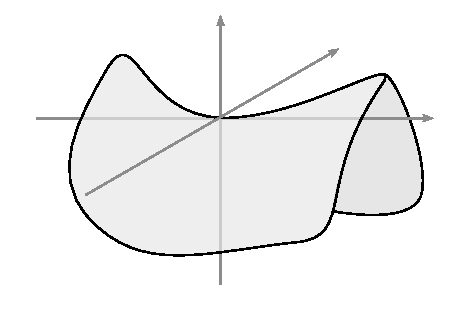
\includegraphics{img/16_quadric.pdf}
      \caption{Quadric}
      \label{img:quadric}
    \end{center}
  \end{figure}
\end{example}

\begin{theorem}
   Let $A \geq 0$. Then $\exists! B \geq 0: B^2 = A$.
   \[ B \coloneqq A^{\frac12} \]
\end{theorem}

\begin{proof}
  We prove the existence of $B$.

  $A$ is self-adjoint, so there exists a unitary matrix $U$ such that $U^* AU = \operatorname{diag}(\lambda_1, \dots, \lambda_n)$
  with all $\lambda_i \geq 0$.
  \[ A = U \begin{bmatrix} \lambda_1 & & \\ & \ddots & \\ & & \lambda_n \end{bmatrix} U^* \]
  \[ B = U \begin{bmatrix} +\sqrt{\lambda_1} & & \\ & \ddots & \\ & & +\sqrt{\lambda_n} \end{bmatrix} U^* \]
  $M \geq 0 \implies C^* MC' \geq 0$.
  $B$ satisfies the condition $B^2 = A$ with $B \geq 0$.

  Conditionless $B \geq 0$: $\leadsto 2^{\rank(A)}$ different solutions.

  We prove uniqueness of $B$.

  Let $B \geq 0$ and $B^2 = a$.
  Let $u_1, \dots, u_n$ be orthonormal basis of eigenvectors for eigenvalues $\mu_1, \dots, \mu_n$ of $B$ with $\lambda_i \geq 0$.
  \[ \implies Bu_i = \mu_i u \qquad \mu_i \geq 0 \]
  \[ Au_i = B^2 u_i = \mu_i^2 u_i \implies \mu_i^2 = \lambda_i \implies \mu_i = +\sqrt{\lambda_i} \]
  \[
    \implies U^* BU = \begin{bmatrix} \mu_1 & & \\ & \ddots & \\ & & \mu_n \end{bmatrix}
    \land    U^* AU = \begin{bmatrix} \lambda_1 & & \\ & \ddots & \\ & & \lambda_n \end{bmatrix}
  \]
\end{proof}

\begin{Remark}[Another solution]
  Find $B$ such that $B^* B = A$. There are infinitely many solutions.
\end{Remark}

\subsection{Cholesky decomposition}

\begin{Person}
  Andr\'e-Louis Cholesky (1875--1918) descending from the Cholewski (Polish) family
\end{Person}

\index{Cholesky decomposition}
\begin{theorem}[Cholesky decomposition] % Satz 12.17
  Let $A > 0 \iff \exists C \in \mathbb C^{n \times n}$ (lower triangular matrix) such that $A = C \cdot C^*$ and $C$ has positive diagonal entries.
  Compare with LU decomposition.
\end{theorem}

\begin{Remark}[Algorithm]
  Determine the matrix $C$ or abort if $A$ is not positive definite.
\end{Remark}

\index{Schur complement}
\begin{Remark}[Schur complement]
  \[ M = \begin{bmatrix} A & B \\ C & D \end{bmatrix} \]
  \[ \implies M/D \coloneqq A - BD^{-1} C \]
  is the Schur complement of block $D$ in $M$ where $M$ is a $(p + q) \times (p + q)$ matrix and $M/D$ is a $p\times p$ matrix.
\end{Remark}

\begin{lemma} % 12.18
  Let $A \in \mathbb C^{n \times n}$. $A > 0$, $b \in \mathbb C^n$, $\gamma > 0$.
  \[ \det\left[\begin{array}{c|c}A & B \\ \hline b^* & \gamma \end{array}\right] = \det A \cdot (\gamma - b^* A^{-1} b)  \]
  \[
    \begin{vmatrix} A & b \\ b^* & \gamma \end{vmatrix}
    = \begin{vmatrix} I & 0 \\ -b^* A^{-1} & 1 \end{vmatrix} \cdot \begin{vmatrix} A & b \\ b^* & \gamma \end{vmatrix}
    = \begin{vmatrix} A & b \\ -\underbrace{b^* A^{-1} A + b^*}_{=0} & -b^* A^{-1} b + \gamma \end{vmatrix}
    = \det{A} \cdot (-b^* A^{-1} b + \gamma)
  \]
\end{lemma}

\begin{proof}[Proof by Cholesky]
  By complete induction:
  \begin{description}
    \item[Case $\mathbf{n = 1}$:]
      \[
        [a_{11}] > 0
        \qquad \implies a_{11} > 0
      \]\[
        C = [ e^{i\theta} \sqrt{a_{11}}] \text{ is unique} \qquad
        C^* = [e^{-i\theta} \sqrt{a_n}]
      \]
    \item[Case $\mathbf{k \to k+1}$:]
      \[ A_{k+1} = \begin{bmatrix} A_k & b \\ b^* & \gamma \end{bmatrix} \qquad A_k \in \mathbb C^{n \times n}, A_k > 0 \]
      By induction hypothesis:
      $\exists C_k: A_k = C_k C_k^*$.

      \[ \text{Find } C_{k+1} = \begin{pmatrix} &  & & 0 \\ & C_k & & \vdots \\ & & & 0 \\ & C^* & & \alpha \end{pmatrix} \text{ such that } C_{k+1} C_{k+1}^* = A_{k+1}, \alpha > 0 \]
      \[ C_{k+1} C_{k+1}^* = \begin{bmatrix} &  & & 0 \\ & C_k & & \vdots \\ & & & 0 \\ & C^* & & \alpha \end{bmatrix} \begin{bmatrix} &  & & c \\ & C_k^* & & \\ & & & \\ 0 & \dots & 0 & \alpha \end{bmatrix} = \left[\begin{array}{c|c} C_k C_k^* & C_k \cdot c \\ C^* C_k^* & C^* C + \alpha^2 \end{array}\right]  \overset!= \begin{bmatrix} A_k & b \\ b^* & \gamma \end{bmatrix} \]
      Requirement: $C_k c\dot c = b$. $c^* c + \alpha^2 = \gamma$.
      Choose $c = C_k^{-1} b$.
      \begin{align*}
        \alpha^2 &= \gamma - c^* c
          = \gamma - b^* {C_k^*}^{-1} {C_k}^{-1} b  \\
          &= \gamma - b^* A^{-1} b
          = \frac{\det{A_{k+1}}}{\det{A_k}} > 0
      \end{align*}
      \[ A_k = C_k C^*_k \qquad A_k^{-1} = {C_k^*}^{-1} C_k^{-1} \]
      \[ \implies \alpha = \sqrt{\gamma - b^* A^{-1} b} = \sqrt{\frac{\det{A_{k+1}}}{\det{A_k}}} \]
  \end{description}
\end{proof}

\begin{Remark}[Application]
  Find $C$ such that $C \cdot C^* = A$.
  $c_{ij} = 0$ if $j > i$.
  $c_{ii} > 0$.
  \[
    a_{ij} = \sum_{k=1}^n c_{ik} (c^*)_{kj}
      = \sum_{k=1}^n c_{ik} \overline{c_{jk}}
      = \sum_{k=1}^{\min(i,j)} c_{ik} \overline{c_{jk}}
  \]

  The algorithm fills up columns from top to bottom and the columns are fill from left to right.

  \begin{description}
    \item[1st column] 
      \begin{align*}
        a_{11} &= c_{11} \cdot \overline{c_{11}} = c_{11}^2 \implies c_{11} = \sqrt{a_{11}} \\
        a_{21} &= c_{21} \cdot \overline{c_{11}} = c_{21} \cdot c_{11} \implies c_{21} = \frac{a_{21}}{c_{11}} \\
        a_{31} &= \sum_{k=1}^{\min(3,1)} c_{3k} \overline{c_{jk}} = c_{31} c_{11} \implies c_{31} = \frac{a_{31}}{c_4} \\
        c_{n1} &= \frac{a_{n1}}{c_{11}} = \frac{a_{n1}}{\sqrt{a_{11}}}
      \end{align*}
      \[ c_{11} = \sqrt{a_{11}} \qquad c_{21} = \frac{a_{21}}{\sqrt{a_{11}}} \quad \dots \quad c_{n1} = \frac{a_{n1}}{\sqrt{a_{11}}} \]
    \item[Induction]
      Assume columns $1, \dots, j-1$ are determined, i.e. $c_{ik}$ is known for $k = 1, \dots, j-1$ and $i = 1, \dots, n$.
      \[ a_{ji} = \sum_{k=1}^j c_{jk} \overline{c_{jk}} = \sum_{k=1}^{j-1} \card{c_{jk}}^2 + c_{jj}^2 \]
      \[ \implies c_{jj} = \sqrt{a_{jj} - \sum_{k=1}^{j-1} \card{c_{jk}}^2} \]
      for $i > j$:
      \[ a_{ij} = \sum_{k=1}^j  c_{ik} \overline{c_{jk}} = \sum_{k=1}^{j-1} c_{ik} \overline{c_{jk}} + c_{ij} c_{jj} \]
      \[ c_{ij} = \frac{a_{ij} - \sum_{k=1}^{j-1} c_{ik} \overline{c_{jk}}}{c_{jj}} \]
      where $c_{jj}$ was already determined and the values of the enumerator are already known.
  \end{description}
\end{Remark}

\begin{Remark}
  $A > 0 \iff$ congruent to unit matrix $\iff$ $A$ has full rank.
  See Corollary~\ref{cor829}.
\end{Remark}

\dateref{2018/06/18}

Cholesky decomposition:
\begin{enumerate}
  \item Given $A > 0$
  \item Find $C$ such that $A = CC^*$. Recursively:
    \[ c_{ij} = \sqrt{a_{ii} - \sum_{k=1}^{i-1} \card{c_{ik}}^2} \]
    \[ c_{ij} = \frac{1}{c_{jj}} \left(a_{ij - \sum_{k=1}^{j-1} c_{ik} \overline{c_{jk}}}\right) \]
\end{enumerate}

\begin{example} % Beispiel 12.20
  \[
    A = \begin{bmatrix} 4 & 12 & -16 \\ 12 & 37 & -43 \\ -16 & -43 & 98 \end{bmatrix}
    \overset!= \begin{bmatrix} c_{11} & & \\ c_{21} & c_{22} & \\ c_{31} & c_{32} & c_{33} \end{bmatrix} \cdot \begin{bmatrix} c_{11} & \overline{c_{21}} & \overline{c_{31}} \\ 0 & c_{22} & \overline{c_{32}} \\ 0 & 0 & c_{33} \end{bmatrix}
  \] \[
    = \begin{bmatrix} c_{11}^2 & c_{11} \overline{c_{21}} & c_{11} \overline{c_{31}} \\
    c_{21} c_{11} & \card{c_{21}}^2 + c_{22}^2 & \\
    c_{31} c_{11} & c_{31} \overline{c_{21}} + c_{32} c_{22} & \card{c_{31}}^2 + \card{c_{32}}^2 + c_{33}^2 \end{bmatrix}
  \]
  with
  \begin{align*}
    c_{11} &= \sqrt4 = 2 \\
    12 &= c_{11} \cdot \overline{c_{21}} \implies c_{21} = \frac{12}{c_{11}} = 6 \\
    -16 &= c_{11} \overline{c_{31}} \implies c_{31} = -\frac{16}{c_{11}} = -8 \\
    \card{c_{21}}^2 &= 37 \\
    c_{22} &= \sqrt{37 - 6^2} = 1 \\
    c_{31} \overline{c_{21}} + c_{32} c_{22} &= -43 \\
    c_{32} &= \frac{-43 - c_{31} \overline{c_21}}{c_{22}} = \frac{-43 + 8 \cdot 6}{1} = 5 \\
    \card{c_{31}}^2 + \card{c_{32}}^2 + c_{33}^2 &= 98 \implies c_{33} = \sqrt{98 - (-8)^2 - 5^2} = 3
  \end{align*}
  If some root of a negative number needs to be taken, the matrix was not positive definite.
\end{example}

\begin{remark} % Bemerkung 12.21
  If $A \in \mathbb R^{n \times n}$, then
  \begin{enumerate}
    \item also $C \in \mathbb R^{n \times n}$.
    \item $C$ is uniquely determined.
    \item Cholesky decomposition is an $LU$ decomposition
  \end{enumerate}
\end{remark}

\begin{corollary} % Korollar 12.22
  If $A > 0$, then $\det{A} \leq a_{11} a_{22} \dots a_{nn}$.
\end{corollary}

\begin{proof}
  $A = CC^*$ is a Cholesky decomposition.
  \[ c_{ii} = \sqrt{a_{ii} - \sum_{k=1}^{j-1} \card{c_{ik}}^2} \leq \sqrt{a_{ii}} \]
  We apply the product law.
  \begin{align*}
    \det(A) &= \det(C C^*) \\
      &= \det(C) \cdot \det(C^*) \\
      &= \card{\det(C)}^2 \\
      &= \card{\prod_{i=1}^n c_{ii}}^2 = \prod c_{ii}^2 \leq \prod a_{ii}
  \end{align*}
\end{proof}

\begin{Person}
  J. S. Hadamard (1865--1963)
\end{Person}

\index{Hadamard's inequality}
\begin{corollary}[Hadamard's inequality] % Korollar 12.23
  Let $A \in \mathbb C^{n \times n}$ with column vectors $a_1, \dots, a_n$.
  \[
    \card{\det{A}} \leq \prod_{i=1}^n \norm{a_{i}} \qquad
    \norm{a_i} \coloneqq \sqrt{\angel{a_i, a_i}} = \sqrt{a_i^* \cdot a_i} = \text{ Euclidean norm}
  \]
\end{corollary}

\begin{proof}
  \begin{description}
    \item[Case 1:] $A$ is singular, thus trivial ($\det(A) = 0$).
    \item[Case 2:] $A$ is invertible $\implies B = A^* A$ is invertible $\implies$ positive definite.
  \end{description}%
  \begin{align*}
    \det{B} &\leq \prod_{i=1}^n b_{ii} = \det(A^* A) = \card{\det{A}}^2 \\
    b_{ii}  &= \text{ i-th row of $A^*$ } \times \text{ i-th colum of $A$ } = a_i^* \cdot a_i = \norm{a_i}^2 \\
    \implies \card{\det{A}}^2 &\leq \prod_{i=1}^n \norm{a_i}^2
  \end{align*}
\end{proof}

In this chapter: $AA^* = A^* A$. \\
There exists an orthonormal basis of eigenvectors:
\begin{align*}
  Ax_i &= \lambda_i x_i \\
  \angel{x_i, x_j} &= \delta_{ij} \\
  x \in \mathbb C^n \leadsto x &= \sum \alpha_i x_i \qquad \alpha_i = \angel{x, x_i} \\
  Ax &= \sum \alpha_i Ax_i = \sum \alpha_i \lambda_i x_i \\
    &= \sum \lambda_i \angel{x, x_i} x_i \\
  \implies A &= \sum_{i=1}^n \lambda \angel{\cdot, x_i} x_i
\end{align*}
where $\cdot$ is a placeholder. It represents the map $\angel{\cdot, x_i}: \mathbb C^n \to \mathbb C$ with $x \mapsto \angel{x, x_i}$.

\begin{Remark}
  Let $z \in \mathbb C$.
  \[ z = r \cdot e^{i \theta} \]
  \begin{align*}
    r &= \card{z} = \sqrt{z \overline{z}} \\
    e^{i \theta} &= \frac{z}{\card{z}}
  \end{align*}
\end{Remark}

\index{Polar decomposition}
\begin{theorem}[Polar decomposition] % Satz 12.24
  Let $A \in \mathbb C^{n \times n}$.
  \[ \card{A} \coloneqq (A^* A)^{\frac12} \qquad (\text{unique, positive semidefinite root}) \]
  Then $\exists U \in \mathcal U(n)$ such that $A = U \cdot \card{A}$.
\end{theorem}

\begin{proof}
  \begin{description}
    \item[Case 1: $A$ is invertible]
      $A A^*$ is positive definite.
      \[ \leadsto A^* A = V \begin{bmatrix} \lambda_1 & &  \\ & \ddots & \\ & & \lambda_n \end{bmatrix} V^* \qquad \lambda_i > 0 \]
      \[ \card{A} \coloneqq (A^* A)^{\frac12} = V \begin{bmatrix} \sqrt{\lambda_1} & &  \\ & \ddots & \\ & & \sqrt{\lambda_n} \end{bmatrix} V^* \]
      \[ U = A \cdot \card{A}^{-1} \text{ is unitary} \]
      \[ U = A \cdot (A^* A)^{-\frac12} \]
      \[ U^* U = (A(A^* A)^{-\frac12})^* (A (A^* A)^{-\frac12}) = ((A^* A)^{-\frac12} \cdot A^*) (A (A^* A)^{-\frac12}) = (A^* A)^{-\frac12} (A^* A) (A^* A)^{-\frac12} \]
      \[ = V \begin{bmatrix} \lambda_1^{-\frac12} & & \\ & \ddots & \\ & & \lambda_n^{-\frac12} \end{bmatrix} V^* V \begin{bmatrix} \lambda_1 & & \\ & \ddots & \\ & & \lambda_n \end{bmatrix} V^* V \begin{bmatrix} \lambda_1^{-\frac12} & & \\ & \ddots & \\ & & \lambda_n^{-\frac12} \end{bmatrix} V^* = V \begin{bmatrix} 1 & & \\ & \ddots & \\ & & 1 \end{bmatrix} V^* = I \]
      \[ U \cdot \card{A} = A \cdot \card{A}^{-1} \cdot \card{A} = A \]
    \item[Case 2: $A$ is singular] Incomprehensible.
      Let $A^* A \geq 0$ and some $\lambda_i = 0$.
      By change of basis, $A = V \operatorname{diag}(\lambda_1, \dots, \lambda_k, 0, \dots, 0) V^*$.
      \[ \card{A} = V \operatorname{diag}(\lambda_1^{\frac12}, \dots, \lambda_k^{\frac12}, 0, \dots, 0) V^* \]
      \[ \card{A} = \begin{bmatrix} P & \\ & 0 \end{bmatrix} \qquad U = V \begin{bmatrix} P^{-1} & \\ & 0 \end{bmatrix} \simeq \begin{bmatrix} \tilde U & \\ & I \end{bmatrix} \]
      \[ \implies A = U \card{A} \]
  \end{description}
\end{proof}

\subsection{Singular value decomposition}

\index{Singular value decomposition}
\begin{Remark}[Singular value decomposition]
  \[ A \in \mathbb C^{n \times n} \qquad A = U (A^* A)^{\frac12} \qquad U \text{ unitary} \]
  \[ (A^* A)^{\frac12} \geq 0 \text{ with eigenvalue } s_i \geq 0 \text{ called singular values of } A \]
  \[ (A^* A)^{\frac12} = \sum s_i \angel{\cdot, x_i} x_i \text{ where } x_i \text{ is an orthonormal basis} \]
  \begin{align*}
    A &= U \cdot (A^* A)^{\frac12}
      = \sum_{i=1}^n s_i \angel{\cdot, x_i} \overbrace{U_{x_i}}^{\eqqcolon y_i}
      = \sum_{i=1}^n s_i \angel{\cdot, x_i} y_i \\
    y_i &= U x_i \text{ is also an orthonormal basis} \\
    A \cdot y_i &= s_i \cdot x_i \to \text{ numerically stable} \\
    A^{-1} &= \sum s^{-1}_i \angel{\cdot, y_i} x_i
  \end{align*}
\end{Remark}

\begin{Remark}
  Singular value decomposition is numerically stable and therefore very desirable.

  It furthermore has a very important application in medicine: CT scans.
  Inside the CT tube, X-rays are sent from all directions to all directions.
  You can only determine how much the 

  \[ \int_{\gamma} f(x(t), y(t)) \,dt = Rf(\psi, \Theta) \]
  Is linear: $R(f_1 + f_2) = Rh + Rf_2$.
  Radon transformation. $\lambda_i \to 0$.

  You need to invert the integral. The SVD is the only numerically stable method to achieve it. Other methods will trigger numerical errors that will amplify and therefore give wrong images.
\end{Remark}

\section{Eigenvalue estimates} % Chapter 8

\index{Numerical range}
\index{Numerical radius}
\begin{definition} % Definition 13.1
  Let $A \in \mathbb C^{n \times n}$.
  \begin{align*}
    W(A) &= \setdef{\angel{Ax, x}}{\norm{x} = 1} \subseteq \mathbb C \text{ is called \emph{numerical range of }} A \\
    w(A) &= \sup\setdef{\card{z}}{z \in W(A)} \text{ is called \emph{numerical radius of}} A
  \end{align*}
\end{definition}

\begin{lemma}
  \[ \operatorname{spec}(A) \subseteq W(A) \]
\end{lemma}
\begin{proof}
  $\lambda \in \operatorname{spec}(A)$, eigenvector $x$ such that $Ax = \lambda x$, $\norm{x} = 1$.
  \[ \implies \angel{Ax, x} = \angel{\lambda x, x} = \lambda \in W(A) \]
\end{proof}

\begin{theorem}[Theorem by Toeplitz-Hausdorff]
  $W(A)$ is convex.
\end{theorem}
\begin{Remark}
  The following implications are left as an exercise to the reader:
  $A$ is normal $\implies W(A) = \underbrace{\text{convex } \operatorname{spec}(A)}_{\text{convex hull}} = \setdef{\sum_{i=1}^n \alpha_i \underbrace{\lambda_i}_{\text{eigenvalue}}}{0 \leq \alpha_i \leq 1, \sum \alpha_i = 1} =$ convex set that contains $\operatorname{spec}(A)$.
\end{Remark}

\begin{Person}
  J. W. Strutt (1842--1919) aka 3rd Lord Rayleigh
\end{Person}

\begin{Person}
  W. Ritz (1878--1909), discovered the element Argon ($\rightarrow$ Nobel prize)
\end{Person}

\subsection{Rayleigh--Ritz Theorem}

\begin{theorem}[Rayleigh--Ritz Theorem] % Satz 13.4
  \label{rrthm}
  Let $A \in \mathbb C^{n \times n}$ be self-adjoint.
  $\lambda_1 \leq \lambda_2 \leq \dots \leq \lambda_n$.
  Then
  \[ \lambda_1 = \min_{x \neq 0}\underbrace{\frac{\angel{Ax, x}}{\angel{x, x}}}_{\text{Rayleigh quotient}} = \min\setdef{\angel{Ax, x}}{\norm{x} = 1} = \min{W(A)} \]
  \[ \vdots \]
  \[ \lambda_n = \max_{x \neq 0}\frac{\angel{Ax, x}}{\angel{x, x}} = \max\setdef{\angel{Ax, x}}{\norm{x} = 1} = \max{W(A)} \]
  where
  \[ A = A^* \implies \angel{Ax, x} = \angel{x, Ax} = \overline{\angel{Ax, x}} \]
\end{theorem}

\begin{proof}
  $\lambda_1, \lambda_n \in W(A)$ because $\operatorname{spec}(A) \subseteq W(A)$.
  \[ \implies \min{W(A)} \leq \lambda_1 \qquad \max{W(A)} \geq \lambda_n \]
  Show that $\forall x: \lambda_1 \leq \frac{\angel{Ax, x}}{\angel{x, x}} \leq \lambda_n$.

  Let $u_1, \dots, u_n$ be an orthonormal basis of eigenvectors.
  Let $x \in \mathbb C^n$, $\norm{x} = 1$. $x = \sum_{i=1}^n \alpha_i x_i \implies \norm{x}^2 = \sum_{i=1}^n \card{\alpha_i}^2 = 1$.
  \begin{align*}
    \angel{Ax, x} &= \angel{A \sum \alpha_i x_i, \sum \alpha_j x_j} \\
      &= \angel{\sum \alpha_i \lambda_i x_i, \sum \alpha_j x_j} \\
      &= \sum_{i} \sum_{j} \lambda_i \alpha_i \overline{\alpha}_j \angel{x_i, x_j} \text { with } \angel{x_i, x_j} = \delta_{ij} \\
      &= \sum_{i} \lambda_i \card{\alpha_i}^2  & \leq \max(\lambda_i) \sum \card{\alpha_i}^2 = \max{\lambda_i} \\
      &                                        &\geq \min(\lambda_i) \sum \card{\alpha_i}^2 = \min{\lambda_i}
  \end{align*}
\end{proof}

\begin{remark} % 13.5
  How can we obtain the other eigenvalues?

  For $x \in \mathcal L(u_2, \dots, u_n)$, $\angel{Ax, x} \geq \lambda_2 \norm{x}^2$. \\
  For $x \in \mathcal L(u_1, \dots, u_{n-1}) = \setdef{x}{\angel{x, u_n} = 0} = \set{u_n}^\bot$, $\angel{Ax, x} \leq \lambda_{n-1}$.
\end{remark}

\begin{Person}
  Richard Courant (1888--1972) \\
  E. Fischer (1875--1954) \\
  H. Weyl (1885--1955)

  All of them worked in Göttingen, Germany.
\end{Person}

\subsection{Courant--Fischer--Weyl min--max principle}

\begin{theorem}[Courant--Fischer--Weyl min--max principle] % 13.6
  \label{cfw-mm}
  Let $A \in \mathbb C^{n \times n}$ be self-adjoint.
  \[ \lambda_1 \leq \lambda_2 \leq \dots \leq \lambda_n \]
  Then it holds that
  \begin{enumerate}
    \item $\lambda_k = \max_{\substack{W \subseteq V \\ \dim{W} = k - 1}} \min_{x \in W^\bot \setminus \set{0}} \frac{\angel{Ax, x}}{\angel{x, x}}$. \\
    Special case $k = 1$: $W = \set{0} \to \lambda_i = \min_x \frac{\angel{Ax, x}}{\angel{x, x}}$.
    \item $\lambda_{n+1 - k} = \min_{\substack{W \subseteq V \\ \dim{W} = k-1}} \max_{x \in W^\bot \setminus \set{0}} \frac{\angel{Ax, x}}{\angel{x, x}}$. \\
    Special case $k = 1$: $\lambda_n = \max_x \frac{\angel{Ax, x}}{\angel{x, x}}$.
  \end{enumerate}
  This theorem is more generic than the Rayleigh--Ritz Theorem.
\end{theorem}

\begin{proof}
  For $W \subseteq V$.
  Let $m_A(W) = \min\setdef{\frac{\angel{Ax, x}}{\angel{x, x}}}{x \in W^\bot \setminus \set{0}}$.
  For vectors $m_A(w_1, \dots, w_k) = m_A(\mathcal L(w_1, \dots, w_k))$.
  For some orthonormal basis $u_1, \dots, u_n$ of eigenvectors,
  \[ \lambda_k = m_A(u_1, \dots, u_{k-1}) \overset{\substack{\text{see proof of} \\ \text{Theorem~\ref{rrthm}}}}{=} \min \setdef{\frac{\angel{Ax, x}}{\angel{x, x}}}{x \in \mathcal L(u_k, \dots, u_n)} \]
  with $\mathcal L(u_k, \dots, u_n) = \set{u_1, \dots, u_{k-1}}^\bot$.
  \[ \implies \lambda_k \leq \max_{\substack{W \subseteq V \\ \dim{W} = k - 1}} m_A(W) \]
  Show that: $\forall W \subseteq V$ with $\dim(W) = k-1$, $m_A(w) \leq \lambda_k$.
  \[ \dim{W^{\bot}} = n - k + 1 \implies W^\bot \cap \mathcal L(u_1, \dots, u_k) \neq \set{0} \]
  \[ v = \sum_{i=1}^k \alpha_i u_i \in W^\bot \cap \mathcal L(u_1, \dots, u_k) \text{ with } \norm{v} = 1 \]

  \[ \angel{Av, v} = \sum_{i=1}^k \card{\alpha_i}^2 \cdot \lambda_i \leq \lambda_k \underbrace{\sum \card{\alpha_i}^2}_{=1} = \lambda_k \]
  \[ m_A(w) = \min_{x \in W^\bot} \angel{Ax, x} \leq \angel{Av, v} = \lambda_k \]
\end{proof}

\dateref{2018/06/20}

The Rayleigh-Ritz coefficient gives us $\lambda_1 = \min_{\angel{x,x} = 1} \angel{Ax, x} = \min{W(A)}$ and $\lambda_n = \max_{\angel{x,x} = 1} \angel{Ax, x}$ with $A = A^*$ and $\lambda_1 \leq \lambda_2 \leq \dots \leq \lambda_n$. $x = \sum \alpha_i u_i$ with $\sum \card{\alpha_i}^2 = 1$ is an orthonormal basis $u_1, \dots, u_n$ of eigenvectors. $\angel{Ax, x} = \sum_1^n \lambda_i \card{\alpha_i}^2$. For $x \in \mathcal L(u_2, \dots, u_n) \to \geq \lambda_2$.

This is used by the Courant--Fischer--Weyl min--max principle.

\begin{enumerate}
  \item First statement:
    \[ \lambda_k = \max_{\substack{W \leq V \\ \dim{W} = k-1}} \min_{\substack{x \in W^\bot \\ \angel{x, x} = 1}} \angel{Ax, x} \]
  \item Second statement:
    \[ \lambda_{n+1-k} = \min_{\substack{W \leq V \\ \dim{W} = k-1}} \max_{\substack{x \in W^\bot \\ \angel{x,x} = 1}} \angel{Ax, x} \]
\end{enumerate}

\begin{proof}[Proof of Theorem~\ref{cfw-mm} continued]
  The second statement follows from the first:
  $-A$ has eigenvalues: $-\lambda_n \leq -\lambda_{n-1} \leq \dots \leq -\lambda_{2} \leq -\lambda_1$.

  We apply the first statement on $-A$.
  \begin{align*}
    \underbrace{\lambda_k(-A)}_{-\lambda_{n+1-k}} &= \max_{\substack{W \subseteq V \\ \dim{W} = k-1}} \min_{\substack{x \in W^\bot \\ \angel{x, x} = 1}} \angel{-Ax, x} \\
      &= \max_{\substack{W\subseteq V \\ \dim{W} = k-1}} \left(- \max_{\substack{x \in W^\bot \\ \angel{x, x} = 1}} \angel{Ax, x}\right) \\
      &= -\min_{\substack{W \subseteq V \\ \dim{W} = k-1}} \max_{\substack{x \in W^\bot \\ \angel{x, x} = 1}} \angel{Ax, x}
  \end{align*}
\end{proof}

\subsection{Cauchy interlacing theorem}

\begin{corollary}[Cauchy interlacing theorem (dt. \foreignlanguage{german}{Schachtelungssatz von Cauchy})] % Korollar 13.7
  Let $A \in \mathbb C^{n \times n}$, $A = A^*$. $\lambda_1 \leq \lambda_2 \leq \dots \leq \lambda_n$.
  Let $B = [a_{ij}]_{i,j=1,\dots,n-1}$. Thus, the last row and column was removed. The dimension is reduced by 1.
  $B = B^*$.
  Eigenvalues: $\mu_1 \leq \mu_2 \leq \dots \leq \mu_{n-1}$.
  Then it holds that $\lambda_1 \leq \mu_1 \leq \lambda_2 \leq \mu_2 \leq \lambda_3 \leq \dots \leq \lambda_{n-1} \leq \mu_{n-1} \leq \lambda_n$.
  In general: If $P$ is an orthogonal projection on a subspace of dimension $n-1$.

  For example,
  \[ P = \begin{bmatrix} 1 & & & \\ & \ddots & & \\ & & 1 & \\ & & & 0 \end{bmatrix} \]
  then the eigenvalues (except for eigenvalue $0$) of $PAP$ are nested like above.
\end{corollary}

\begin{proof}
  \[
    A = \begin{bmatrix}
      [B] & b \\
      b^* & \gamma
    \end{bmatrix}
  \]
  Let $w_1, \dots, w_{n-1} \in \mathbb C^{n-1}$ be an orthonormal basis of eigenvectors of $B$.
  \[ Bw_i = \mu_i w_i \qquad u_i = \vectwo{w_i}{0} \in \mathbb C^n \qquad u_n = \begin{pmatrix} 0 \\ \vdots \\ 0 \\ 1 \end{pmatrix} \]
  $\leadsto u_1, \dots, u_{n-1}, u_n$ is an orthonormal basis of $\mathbb C^n$. Attention! There is no eigenvector of $A$.
  \[ W_k = \mathcal L(u_1, \dots, u_{k-1}, u_n) \]
  \[
    \text{By Theorem~\ref{cfw-mm} } \implies
    \lambda_{k+1} = \max_{\substack{W \subseteq \mathbb C^n \\ \dim{W} = k}} \min_{x \in W^\bot \setminus \set{0}} \frac{\angel{Ax, x}}{\angel{x, x}} \geq \min_{x \in W_k^\bot \setminus \set{0}} \frac{\angel{Ax, x}}{\angel{x, x}}
  \]
  \[ x \in W_k^\bot \iff \angel{x, u_i} = 0 \qquad i = 1, \dots, k-1 \land \angel{x, u_n} = x_n = 0 \]
  \[ \iff x = \begin{bmatrix} y \\ 0 \end{bmatrix}, y \in \set{w_1, \dots, w_{k-1}}^\bot \underbrace{=}_{w_1, \dots, w_{n-1} \text{ is ONB of } \mathbb C^{n-1}} \mathcal L(w_k, \dots, w_{n-1}) \subseteq \mathbb C^{n-1} \]
  \[ y = \sum_{i=k}^{n-1} \alpha_i w_i \]
  \[
    \frac{\angel{Ax, x}}{\angel{x, x}}
    = \frac{\angel{\begin{bmatrix} B & b \\ b^* & \gamma \end{bmatrix} \begin{bmatrix} y \\ 0 \end{bmatrix}, \begin{bmatrix} y \\ 0 \end{bmatrix}}}{\angel{\begin{bmatrix} y \\ 0 \end{bmatrix},\begin{bmatrix} y \\ 0 \end{bmatrix}}}
    = \frac{\angel{\begin{bmatrix} B & y \\ b^* & -y \end{bmatrix}, \begin{bmatrix} y \\ 0 \end{bmatrix}}}{\angel{y, y}}
    = \frac{\angel{By, y}}{\angel{y, y}}
  \] \[
    = \frac{\angel{B \sum_{i=k}^{n-1} \alpha_i w_i, \sum_{j=k}^{n-1} \alpha_j w_j}}{\sum_{i=1}^{n-1} \card{\alpha_i}^2}
    = \frac{\sum_{i=k}^{n-1} \mu_i \card{\alpha_i}^2}{\sum_{i=1}^{n-1} \card{\alpha_i}^2} \geq \mu_k
  \]
  Inversion:
  $-A$ has eigenvalues $-\lambda_n \leq -\lambda_{n-1} \leq \dots \leq -\lambda_2 \leq -\lambda_1$.
  $-B$ has eigenvalues $-\mu_{n-1} \leq -\mu_{n-2} \leq \dots \leq -\mu_2 \leq -\mu_1$.

  We apply step 1 on $-A$ and $-B$:
  \[ \lambda_{k+1} (-A) \geq \lambda_k (-B) \]
  \[ -\lambda_{n-k} \geq -\mu_{n-k} \]
  \[ \implies \lambda_{n-k} \leq \mu_{n-k} \quad \forall k = 1, \dots, n-1 \]
  \[ \implies \lambda_k \leq \mu_k \quad \forall k \forall k = 1, \dots, n-1 \]
\end{proof}

\begin{corollary} % Korollar 13.8
  \label{col138}
  $A, B$ are self-adjoint $\in \mathbb C^{n \times n}$.
  \[ \lambda_{k}(A) + \lambda_1(B) \leq \lambda_k(A + B) \leq \lambda_k(A) + \lambda_n(B) \]
\end{corollary}
\begin{proof}
  \[ \lambda_1(B) \leq \frac{\angel{Bx, x}}{\angel{x, x}} \leq \lambda_n(B) \]
  because of Theorem~\ref{rrthm}.
  \[ \lambda_k(A + B) = \max_{\dim{W}=k-1} \min_{x \in W^\bot \setminus \set{0}} \frac{\angel{(A + B)x, x}}{\angel{x, x}} \]
  \[ \frac{\angel{Ax, x}}{\angel{x, x}} + \lambda_1(B) \leq \frac{\angel{(A + B)x, x}}{\angel{x, x}} \leq \frac{\angel{Ax, x}}{\angel{x, x}} + \lambda_n(B) \]
  This goes on and on $\leadsto \lambda_k(A) + \lambda_l(B)$.
  \[ \leq \lambda_l(A) + \lambda_n(B) \]
\end{proof}

\begin{corollary} % Folgerung 13.9
  If $B \geq 0$, $A = A^*$, then $\lambda_k(A) \leq \lambda_k(A + B) \forall k$.
\end{corollary}

\begin{Person}
  Sem\"en Aranovi\v{c} Ger\v{s}gorin (1901--1933)
\end{Person}

\subsection{Ger\v{s}gorin theorem}

\index{Ger\v{s}gorin disc}
\index{Ger\v{s}gorin Theorem}
\begin{theorem}[Ger\v{s}gorin Theorem] % 13.10
  Let $A \in \mathbb C^{n \times n}$.
  \[
    \begin{bmatrix}
      \card{a_{11}} & \card{a_{12}} & \dots  & \card{a_{1n}} \\
      \card{a_{21}} & \card{a_{22}} & \dots  & \card{a_{2n}} \\
      \vdots        &               & \ddots & \vdots \\
      \card{a_{n1}} & \card{a_{n2}} & \dots  & \card{a_{nn}}
    \end{bmatrix}
    \quad \to \quad
    r_i = \sum_{\substack{j=1 \\ j\neq i}}^n \card{a_{ij}}
    \quad \to \quad
    \begin{bmatrix}
      \sum_{j\neq 1} \card{a_{1j}} \\
      \sum_{j\neq 2} \card{a_{2j}} \\
      \vdots \\
      \sum_{j\neq n} \card{a_{nj}}
    \end{bmatrix}
  \]
  So, we remove the diagonal elements and consider the row sum norm.
  This yields the so-called \emph{Ger\v{s}gorin discs}.
  The theorem claims:
  \[
    \operatorname{spec}(A) \subseteq \bigcup_{k=1}^n \setdef{z \in \mathbb C}{\card{z - a_{ii}} \leq r_{i}}
  \]
\end{theorem}

\begin{proof}
  Show that $\forall \lambda \in \operatorname{spec}(A) \exists i: \card{\lambda - a_{ii}} \leq r_i$.
  Let $x$ be an eigenvector: $Ax = \lambda x$.
  Without loss of generality: $\max_i \card{x_i} = 1$.
  Hence $\forall j: \card{x_j} \leq 1$ and $\exists i: \card{x_i} = 1$.
  \[ \underbrace{(Ax)_i}_{\sum_j a_{ij} x_j} = \lambda \cdot x_i \text{ because it is an eigenvector} \]
  \[ \implies \sum_{\substack{j = 1 \\ j \neq i}}^n a_{ij} x_j = \lambda x_i - a_{ii} x_i \qquad
     \implies \underbrace{\card{\lambda x_i - a_{ii} x_i}}_{= \card{\lambda - a_{ii}} \cdot \card{x_i}} = \card{\sum_{j \neq i} a_{ij} x_j} \]
  \[ \card{\lambda - a_{ii}} \cdot \underbrace{\card{x_i}}_{=1} \leq \sum_{j \neq i} \card{a_{ij}} \underbrace{\card{x_j}}_{\leq 1} \]
  \[ \card{\lambda - a_{ii}} \leq \sum_{j \neq i} \card{a_{ij}} = r_i \]
\end{proof}

\begin{remark} % Bemerkung 13.11
  For dimension greater $5$, it becomes infeasible to determine the characteristic polynomial to retrieve the eigenvalues.

  In theory:
  \begin{enumerate}
    \item $\chi_A(x) = \det(x \cdot I - A)$ (difficult if precision is necessary)
    \item find roots (cumbersome or infeasible)
    \item find eigenvectors (numerically unstable)
  \end{enumerate}

  In practice, we apply an iterative approach:
  \begin{description}
    \item[Given] A
    \item[Find] $x$ such that $Ax = \lambda x$, $A^2 x = \lambda Ax$, $A^3 x = \lambda A^2 x \leadsto A^\infty x = \lambda A^\infty x$ then $A^\infty x$ is eigenvector. As mathematicians we need to ask ourselves, whether $A^\infty x$ converges? The answer is no, not always. We need to fix $x$ to converge to infinity, not $0$.

    Choose initial vector $x_0$ with $\norm{x_0} = 1$.
    \[ w_{k+1} = Ax_k \qquad x_{k+1} = \frac{w_{k+1}}{\norm{w_{k+1}}} \qquad \implies \forall n: \norm{x_n} = 1 \]
    Thus we achieved that all the points lie inside the unit sphere.
    By the Heine-Borel Theorem, a sequence in a bounded and closed (thus compact) space has a convergent subsequence.

    \begin{claim}
      $x_n$ converges assuming $\card{\lambda_1} > \card{\lambda_2} \geq \dots \geq \card{\lambda_n}$ and $A$ diagonalizable.
    \end{claim}
    Let $v_1, \dots, v_n$ be a basis of eigenvectors.
    \[ x_0 = \alpha_0 v_1 + \dots + \alpha_n v_n \]
    \[ x_k = \frac{A^k x_0}{\norm{A^k x_0}} \]
    converges towards $v_1$.
    \[ A^k v_i = \lambda_i^k v_i \]
    \begin{align*}
      A^k x_0 &= \alpha_1 A^k v_1 + \dots + A^k v_n \\
          &= \alpha_1 \lambda_1^k v_1 + \alpha_2 \lambda_2^k v_2 + \dots + \alpha_n \lambda_n^k v_n \\
      x_k &= \frac{A^k x_0}{\norm{A^k x_0}} = \frac{\alpha_1 \lambda_1^k v_1 + \alpha_2 \lambda_2^k v_2 + \dots + \alpha_n \lambda_n^k v_k}{\norm{\alpha_1 \lambda_1^k v_1 + \alpha_2 \lambda_2^k v_2 + \dots + \alpha_n \lambda_n^k v_n}} \\
          &= \frac{\lambda_1 \cdot \lambda_1^k}{\card{\alpha_1 \cdot \lambda_1^k}} \cdot
            \frac{v_1 + \frac{\alpha_2}{\alpha_1} \left(\frac{\lambda_2}{\lambda_1}\right)^k v_2 + \dots + \frac{\alpha_n}{\alpha_1} \left(\frac{\lambda_n}{\lambda_1}\right)^k v_n}{\norm{v_1 + \frac{\alpha_2}{\alpha_1} \left(\frac{\lambda_2}{\lambda_1}\right)^k v_2 + \dots + \frac{\alpha_n}{\alpha_1} \left(\frac{\lambda_n}{\lambda_n}\right)^k v_n}} \\
          &\overset{k \to \infty}\approx \frac{\alpha_1 \lambda_1^k}{\card{\lambda_1^k}} \cdot v_1 \text{ because }
          \card{\lambda_i} > \card{\lambda_1} \forall i \geq 2 \implies \frac{\card{\lambda_i}}{\card{\lambda_1}} < 1
    \end{align*}
    The smaller $\frac{\card{\lambda_2}}{\card{\lambda_1}}$ is, the faster it converges.
    \[ \left(\frac{\card{\lambda_1}}{\card{\lambda_i}}\right)^k \xrightarrow{k \to \infty} 0 \]
  \end{description}

  \emph{Spectral gap}\index{Spectral gap} is the difference between the moduli of the two largest eigenvalues of a matrix.
\end{remark}

\section{Matrix norms}
\index{Matrix norm}
\[ \norm{x} = \sqrt{\angel{x, x}} \]

Norm on a vector space is a map $\norm{\cdot}: V \to [0, \infty[$:
\begin{enumerate}
  \item $\norm{v} = 0 \iff v = 0$
  \item $\norm{\lambda v} = \card{\lambda} \cdot \norm{v}$
  \item $\norm{v + w} \leq \norm{v} + \norm{w}$
\end{enumerate}

\index{Compatible norms}
\begin{definition} % Definition 14.1
  Let $V, W$ be vector spaces with norms $\norm{\cdot}_V$ and $\norm{\cdot}_W$.
  A norm on $\operatorname{Hom}(V, W)$ is \emph{compatible} with $\norm{\cdot}_V$ and $\norm{\cdot}_W$ if
  \[ \forall v \in V \forall f \in \operatorname{Hom}(V, W): \norm{f(v)}_W \leq \norm{f} \cdot \norm{v}_V \]
  \[ v = x - y \implies \norm{f(x) - f(y)}_W = \norm{f(x - y)}_W \leq \norm{f} \cdot \norm{x - y}_V \]
  Hence $f$ is Lipschitz continuous with constant $\leq \norm{f}$.
  Specifically, we define the Lipschitz constant uniquely with
  \[ \inf\setdef{C}{\norm{f(v)}_W \leq C \cdot \norm{v}_W \forall v \in V} \]
\end{definition}

\begin{example}
  In $\mathbb C^{n \times n}$, one scalar product is defined by $\angel{A, B} \coloneqq \operatorname{Tr}(B^* A)$.
  The Frobenius norm (or Schur norm) (or Hilbert-Schmidt norm) is defined as
  \[ \norm{A}_F \coloneqq \sqrt{\operatorname{Tr}(A^* A)} = \left(\sum_{ij} \card{a_{ij}}^2\right)^{\frac12} \]
  It is compatible with the Euclidean norm on $\mathbb C^n$.

  Let $x \in \mathbb C^n$.
  \begin{align*}
    \norm{Ax}_2^2 &= \sum_{i=1}^n \card{(Ax)_i}^2
      = \sum_{i=1}^n \card{\sum_j a_{ij} x_j}^2 \\
    \text{(CBS inequality, Theorem~\ref{thm:cbs})} &\leq \sum_{i=1}^n \sum_j \card{a_{ij}}^2 \cdot \sum_k \card{x_k}^2
      = \norm{A}_F^2 : \norm{x}_2^2
  \end{align*}
\end{example}

\index{Induced norm}
\begin{lemma} % Lemma 14.3
  Let $V, W$ be normed vectorspaces. $f \in \operatorname{Hom}(V, W)$.
  Then $\norm{f}_{V, W}$ defines a compatible norm and is called \emph{induced norm}.
  \[ \norm{f}_{V,W} \coloneqq \inf\setdef{C}{\norm{f(v)}_W \leq C \cdot \norm{v}_V \forall v \in V} \]
  And specifically,
  \begin{align*}
    \norm{f}_{V,W} &= \sup\setdef{\frac{\norm{f(v)}_W}{\norm{v}}}{v \in V \setminus \set{0}} \\
      &= \sup\setdef{\norm{f(v)}_W}{v \in V, \norm{v} = 1} \\
  \end{align*}
\end{lemma}

\begin{proof}
  \begin{enumerate}
    \item \[ \sup_{v \neq 0} \frac{\norm{f(v)}_W}{\norm{v}_V} = \sup_{\norm{v}_V = 1} \norm{f(v)}_W \text{ is immediate} \]
    \item Let $M_f = \inf\setdef{C}{\norm{f(v)}_W \leq \norm{v}_V \forall v \in V}$. Show that $M_f = \sup_{v \neq 0} \frac{\norm{f(v)}_W}{\norm{v}_V}$.
  \end{enumerate}

  Let $C \geq M_f$. Then $\norm{f(v)}_W \leq C \cdot \norm{v}_V \quad \forall v \in V$.
  \[
    \implies \frac{\norm{f(v)}_W}{\norm{v}_V} \leq C \quad \forall v \neq 0
    \qquad \implies \sup_{v \neq 0} \frac{\norm{f(v)}}{\norm{v}_V} \leq C
    \qquad \implies \sup{\frac{\norm{f(v)}}{\norm{v}}} w \leq M_f
  \]
\end{proof}

\dateref{2018/06/25}

%Matrix norms:
A norm on $\mathbb K^{m \times n}$ (with $\mathbb K = \mathbb C$ or $\mathbb R$) is \emph{compatible} with norms on $\mathbb K^n$ and $\mathbb K^m$ if
\[
  \underbrace{\norm{Ax}_m}_{\substack{\text{vector norm} \\ \text{on } \mathbb K^m}}
  \leq
  \underbrace{\norm{A}_{m \times n}}_{\text{matrix norm}} \cdot \underbrace{\norm{x}_n}_{\substack{\text{vector space} \\ \text{on } \mathbb K^n}}
\]
\[ \norm{A}_F = \operatorname{Tr}(A^* A)^{\frac12} = \left(\sum \card{a_{ij}}^2\right)^{\frac12} \]
is compatible with the Euclidean norm.

Optimal norm on $\mathbb K^{m \times n}$.
\[ \norm A = \inf\setdef{C > 0}{\forall x \in \mathbb K^n: \norm{A \cdot x}_m \leq C \cdot \norm{x}_n} \coloneqq \sup_{\substack{x \\ \norm{x}_n \leq 1}} \norm{Ax}_m \]
\[ f: V \to W \qquad \norm{f} = \sup_{\substack{x \in V \\ \norm{x}_V \leq 1}} \norm{f(x)}_W \]

Exercise for the practicals:
\[ \underbrace{V}_{\norm{\cdot}_V} \xrightarrow f \underbrace{W}_{\norm{\cdot}_W} \xrightarrow g \underbrace{Z}_{\norm{\cdot}} \]

\begin{example} % Beispiel 14.4
  \begin{enumerate}
    \item The Frobeniusnorm $\norm{A}_F = \operatorname{Tr}(A^* A)^{\frac12}$ is not optimal.
      \[
        \operatorname{id}: \mathbb C^n \to \mathbb C^n \qquad
        \norm{\operatorname{id}}_{2 \to 2} = \sup_{\substack{\norm{x} \leq 1 \\ 2}} \norm{x}_2 = 1 \qquad
        \operatorname{id}_F = \norm{I}_F = \operatorname{Tr}(I^2)^{\frac12} = \sqrt n
      \]
    \item The norm induced by the Euclidean norm
      \begin{align*}
        \norm{A}_{2 \to 2} &= \sup\setdef{\norm{Ax}_2}{\norm{x}_2 \leq 1} \\
          &= \sup_{x \neq 0} \frac{\norm{Ax}_2}{\norm{x}_2} = \sup_{x \neq 0} \frac{\angel{Ax, Ax}^{\frac12}}{\angel{x,x}^{\frac12}} \\
          &= \sup_{x \neq 0} \frac{\angel{A^* Ax, x}^{\frac12}}{\angel{x,x}^{\frac12}} = \sqrt{\sup_{x \neq 0} \frac{\angel{A^* Ax, x}}{\angel{x,x}}} \\
          &= \sqrt{\text{largest eigenvalue of } A^* A} = \sqrt{\text{largest singular value of } A}
      \end{align*}
    \item
      $\norm{A}_{\infty\to\infty}$ on $\mathbb K^n: \norm{x}_{\infty} = \max \card{x_i}$ and $\norm{x}_1 = \sum \card{x_i}$.
      \[ \norm{x}_p = \left(\sum_{i=1}^n \card{x_i}^p\right)^{\frac1p} \xrightarrow{p \to \infty} \max \card{x_i} \qquad (1 \leq p \leq \infty) \]
      This convergence is left as an exercise to the reader.
      \[ \norm{A}_{\infty\to\infty} = \sup\setdef{\norm{Ax}_{\infty}}{\norm{x}_\infty \leq 1} \]
      \begin{align*}
        \norm{Ax}_{\infty} &= \max_i \card{(Ax) i} = \max_i \card{\sum_{j=1}^n a_{ij} x_j} \\
          &\leq \max_i \sum_{j=1}^n \card{a_{ij}} \underbrace{\card{x_j}}_{\leq \max_j \card{x_j}}
           \leq \underbrace{\max_j \card{x_j}}_{= \norm{x}_{\infty}} \max_i \sum_{j=1}^n \card{a_{ij}} \\
          &\implies \forall x \in \mathbb K^n: \norm{Ax}_{\infty} \leq \max_i \sum_j \card{a_{ij}} \cdot \norm{x}_{\infty} \\
          &\implies \norm{A}_{\infty\to\infty} \leq \max_i \sum_j \card{a_{ij}}
      \end{align*}
      \begin{claim}
        $\norm{A}_{\infty\to\infty} = \max_i \sum_j \card{a_{ij}}$
      \end{claim}
      \begin{proof}
        Find vector $\tilde x$ such that $\norm{A\tilde x}_{\infty} = \max_i \sum_j \card{a_{ij}} \cdot \norm{\tilde x}_{\infty}$. Choose $i_0$ such that $\sum_i \card{a_{ij}} = \max!$.
        \[ \tilde x_j = \begin{cases} \frac{\card{a_{i_0 j}}}{a_{i_0 j}} & a_{i_0 j} \neq 0 \\ 0 & \text{else} \end{cases} \]
        $\tilde x_j$ are not all zero, $\card{\tilde x_j} \in \set{0,1} \forall j$.
        \begin{align*}
          (A \cdot \tilde x)_{i_0} &= \sum_j a_{i_0 j} \tilde x_j = \sum_j a_{i_0 j} a_{i_0 j} \frac{\card{a_{i_0 j}}}{a_{i_0 j}} = \sum_j \card{a_{i_0 j}} = \max_i \sum \card{a_{ij}} \\
            &\implies \norm{A \tilde x}_{\infty} \geq \card{(A \tilde x)_{i_0}} = \max_i \sum \card{a_{ij}} \cdot \underbrace{\norm{\tilde x}_{\infty}}_{=1} \\
            &\implies \norm{A}_{\infty\to\infty} \geq \max_i \sum_j \card{a_{ij}} \\
            &\implies \norm{A}_{\infty\to\infty} = \max_i \sum_j \card{a_{ij}} = \max\setdef{\norm{z_i}_1}{z_i \text{ row of } A}
        \end{align*}
      \end{proof}
    \item $\norm{A}_{1 \to 1} = \max_j \sum_i \card{a_{ij}}$.
      The proof is left as an exercise to the reader.
  \end{enumerate}
\end{example}

\[ Ax = \lambda x \implies \norm{Ax} = \card{\lambda} \cdot \norm{x} \]
\[ \implies \sup_{x \neq 0} \frac{\norm{Ax}}{\norm{x}} \geq \card{\lambda} \]

\index{Spectral radius}
\begin{definition} % Definition 14.5
  \[
    \rho(A) \coloneqq \max \setdef{\card{\lambda}}{\lambda \in \operatorname{spec}(A)}
    \quad\text{is called \emph{spectral radius} of $A$.}
  \]
\end{definition}

\begin{Remark}
  Why is it called radius? Consider the complex plane. This value is the radius of the smallest circle with center $0$ that contains all eigenvalues.
\end{Remark}

\begin{lemma} % Lemma 14.6
  \begin{enumerate}
    \item For every compatible matrix norm: $\norm{A} \geq \rho(A)$
    \item $\rho(A)$ is not a matrix norm (for some nilpotent matrix, $\rho(A) = 0$ but $A \neq 0$, hence it cannot be a norm)
    \item $\forall A \in \mathbb C^{n \times n} \: \forall \varepsilon > 0 \:\exists \text{ norm on } \mathbb C^n:$ the induced matrix norm satisfies $\norm{A} \leq \rho(A) + \varepsilon$
  \end{enumerate}
\end{lemma}

\begin{proof}[Proof of point 3.]
  \[ \exists \text{ invertible } T \in \mathbb C^{n \times n}: T^{-1} AT = J = \begin{bmatrix} \lambda_1 & \eta_k & & & 0 \\ & \ddots & \eta_{23} & & \\ & & \ddots & \ddots & \\ & & & \ddots & \eta_{n-1,n} \\ 0 & & & & \lambda_n \end{bmatrix} \qquad \eta_{ij} \in \set{0,1} \]
  \[ D_{\varepsilon} = \operatorname{diag}(1, \varepsilon, \varepsilon^2, \dots, \varepsilon^{n-1}) \]
  \[
    D_{\varepsilon}^{-1} J D_{\varepsilon}
      = \operatorname{diag}(1, \frac1\varepsilon, \frac1{\varepsilon^2}, \dots, \frac{1}{\varepsilon^{n-1}})
      \begin{bmatrix} \lambda_1 & \eta_{12} & & \\ & \lambda_2 & \eta_{23} & \\ & & \ddots & \\ & & \lambda_{n-1} & \eta_{n-1,n} \\ & & & \eta_{n} \end{bmatrix}
      \operatorname{diag}(1, \varepsilon, \varepsilon^2, \dots, \varepsilon^{n-1})
  \] \[
      = \begin{bmatrix}
        \lambda_1 & \eta_{12} \varepsilon & & & & \\
          & \frac{\lambda_2}{\varepsilon} \varepsilon \frac{\eta_{23}}{\varepsilon} \varepsilon^2  & & & & \\
          & & \frac{\varepsilon_{3}}{\varepsilon^2} \varepsilon^2 \frac{\eta_{34}}{\varepsilon^2} \varepsilon^3 & & & \\
          & & & \ddots & & \\
          & & & & \ddots & \eta_{n-1} \varepsilon \\
          & & & & & \lambda_n
      \end{bmatrix}
  \]
  Define a norm on $\mathbb C^n$.
  \[ \norm{x}_{\varepsilon} = \norm{D_{\varepsilon}^{-1} T^{-1} x}_{\infty} \]
  \begin{enumerate}
    \item $\norm{x}_{\varepsilon} \geq 0$ is immediate. \\
      $\norm{x}_{\varepsilon} = 0 \implies D_{\varepsilon}^{-1} T^{-1} x = 0 \implies x = 0$
    \item $\norm{\lambda x}_{\varepsilon} = \norm{D_{\varepsilon}^{-1} T^{-1} \lambda x} = \card{\lambda} \cdot \norm{x}_{\varepsilon}$
    \item $\norm{x + y}_{\varepsilon} = \norm{D_{\varepsilon}^{-1} T^{-1} (x + y)}_{\varepsilon} \leq \norm{D_{\varepsilon}^{-1} T^{-1} x}_{\infty} + \norm{D^{-1}_{\varepsilon} T^{-1} y}_{\infty} = \norm{x}_{\varepsilon} + \norm{y}_{\varepsilon}$
  \end{enumerate}
  \[ \norm{A}_{\varepsilon\to\varepsilon} = \sup_{x \neq 0} \frac{\norm{Ax}_{\varepsilon}}{\norm{x}_{\varepsilon}} \]
  \[ x = \underbrace{TD_{\varepsilon}}_{\text{invertible}} y = \sup_{y \neq 0} \frac{\norm{AT D_{\varepsilon} y}_{\varepsilon}}{\norm{TD_{\varepsilon} y}_{\varepsilon}} = \sup_{y \neq 0} \frac{\norm{D_{\varepsilon}^{-1} T^{-1} \left(ATD_{\varepsilon} y\right)}_{\infty}}{\norm{D_{\varepsilon}^{-1} T^{-1} \left(TD_{\varepsilon} y\right)}_{\infty}} = \sup_{y \neq 0} \frac{\norm{J_{\varepsilon} \cdot y}_{\infty}} = \sup_{y \neq 0} \frac{\norm{J_{\varepsilon} y}_{\infty}}{\norm{y}_{\infty}} \]
  \[ \leq \norm{J_{\varepsilon}}_{\infty \to \infty} = \max_i \sum_j \card{(J_{\varepsilon})_{ij}} \leq \underbrace{\max \card{\lambda_i} + \varepsilon}_{= \rho(A) + \varepsilon} \]
\end{proof}

\begin{Person}
  Israel Gelfand (1913--2009)
\end{Person}

\begin{remark} % Bemerkung 14.7
  \[ \rho(A) \leq \norm{A} \]
  \[ \rho(A^2) = \rho(A)^2 \qquad \rho(A^3) = \rho(A)^3 \]
  \[ \operatorname{spec}(A^2) = \setdef{\lambda^2}{\lambda \in \operatorname{spec}(A)} \]
  \[ \max(\card{\lambda_i}^2) = \left(\max\card{\lambda_i}\right)^2 \]

  \[ \rho(A^2) \leq \norm{A}^2 \quad (\leq \norm{A})^2 \]
  \[ \rho(A^3) \leq \norm{A}^3 \qquad \underbrace{\rho(A^k)}_{\rho(A)^k} \leq \norm{A^k} \]
  \[ \implies \rho(A) \leq \norm{A^k}^{\frac1k} \forall k \]
  Geldfand showed:
  \[ \lim_{k\to\infty} \norm{A^k}^{\frac1k} = \rho(A) \]
\end{remark}

\index{Spectral norm}
\begin{lemma} % Lemma 14.8
  \begin{enumerate}
    \item $\norm{A}_{2\to2} = \rho(A^* A)^{\frac12}$ is the \emph{spectral norm}
    \item If $A$ is normal, then $\norm{A}_{2\to2} = \rho(A)$
  \end{enumerate}
\end{lemma}

\begin{proof}
  \begin{enumerate}
    \item Already shown
    \item $\operatorname{spec}(A^* A) = \setdef{\card{\lambda}^2}{\lambda \in \operatorname{spec}(A)}$ is left to be proved by the reader. Then $= \setdef{\overline\lambda \cdot \lambda}{\lambda \in \operatorname{spec}(A)} \implies \rho(A^* A) = \rho(A)^2$
  \end{enumerate}
\end{proof}

\index{Hilbert space}
\begin{remark} % Bemerkung 14.9
  Let $V$ be a vector space with dimension $\infty$ with a norm.
  For example, $l^2 = \setdef{(x_n) \in \mathbb R^\infty}{\sum_1^\infty \card{x_n}^2 < \infty}$
  with norm $\norm{(x_n)} = \left(\sum_1^\infty \card{x_n}^2\right)^{\frac12}$ is a \emph{Hilbert space}.
  \[ l^\infty = \setdef{(x_n)}{\sup\card{x_n} < \infty} \qquad \norm{(x_n)}_{\infty} = \sup\card{x_n} \]
\end{remark}

\begin{Example}
  \[ V = C^{\infty}[0,1] \]
  \[ \frac d{dx}: f \mapsto f' \text{ is linear} \]
  $\norm{\frac{d}{dx}} = \infty$ it does not matter which norm on $C^{\infty}[0,1]$ is defined.
  \[ \rho\left(\frac d{dx}\right) = \infty \qquad f' = \lambda f \qquad f(x) = e^{\lambda x} \in C^\infty \implies \operatorname{spec}\left(\frac{d}{dx}\right) = \mathbb C \]
\end{Example}

\begin{Person}
  Carl Neumann (1832--1925)
\end{Person}

\begin{corollary} % 14.10
  \label{cor1410}
  For compatible norms, if $\norm{A} < 1$ then $I - A$ is invertible and $(I - A)^{-1} = \frac{1}{I - A} = \sum_{n=0}^\infty A^n$ and $\norm{(I - A)^{-1}} \leq \frac{1}{1 - \norm{A}}$

  \begin{enumerate}
    \item $\rho(A) \leq \norm{A} < 1 \implies 1 \not\in \operatorname{spec}(A) \implies I - A$ invertible
    \item Neumann series: $\frac{1}{1 - x} = \sum_{n=0}^\infty x^n$ with $\card{x} < 1$
  \end{enumerate}
\end{corollary}

\begin{Remark}
  \[ y' = \lambda y \qquad \int y' = \lambda \cdot \int y \implies \int y = \frac1{\lambda} \cdot y \]
  Every differentiation can be converted into integration. An integration is bounded ($\lambda$ becomes $\frac1{\lambda}$).
\end{Remark}

\begin{proof}
  $\rho(A) < 1 \implies I - A$ invertible.
  \begin{claim}
    \[ \sum_{n=0}^\infty A^n \text{ converges} \]
  \end{claim}
  \begin{align*}
    \sum{\sum_{n=1}^{N+m} A^n - \sum_{n=1}^N A^n}
      &= \norm{\sum_{n=N+1}^{N+m} A^n} \leq \sum_{n=N+1}^{N+m} \norm{A^n} \leq \sum_{n=N+1}^{N+m} \norm{A}^n \leq \sum_{n=N+1}^\infty \norm{A}^n \\
      &\leq \frac{\norm{A}^{N+1}}{1 - \norm{A}} \xrightarrow{N \to \infty} 0
  \end{align*}
  Thus, the sequence of partial sums is Cauchy and therefore convergent.
  \[ (I - A) \sum_{n=0}^\infty A^n = \sum_{n=0}^\infty A^n - \underbrace{\sum_{n=0}^\infty A^{n+1}}_{= \sum_{n=1}^\infty A^n} = A^0 = I \]
\end{proof}

\[ Ax = \tilde b = b + \text{ error} \]
\[ \tilde x = A^{-1} \tilde b \qquad x = A^{-1} b \qquad \tilde x - x = A^{-1} (\tilde b - b) \implies \norm{\tilde x - x} \leq \norm{A^{-1}} \cdot \norm{\tilde b - b} \]
\[ \norm{\tilde x - x} \overset{\text{?}}\leq C \cdot \norm{\tilde b - b} \]

\begin{corollary} % Korollar 14.11
  Let $A$ be invertible and $B$ be arbitrary with $\norm{B} < \norm{A^{-1}}^{-1}$.
  $\implies A + B$ is invertible and
  \[ \norm{(A + B)^{-1}} \leq \frac{\norm{A^{-1}}}{1 - \norm{A^{-1} \cdot \norm{B}}} \]

  \[ \norm{A} \sim \max\card{\lambda_i} \]
  \[ \norm{A^{-1}} \sim \max\frac{1}{\card{\lambda_i}} = \frac{1}{\min\card{\lambda_i}} \]
  \[ \norm{A^{-1}}^{-1} = \min\card{\lambda_i} \]
  Compare with $A = I$ as special case (this was covered in Corollary~\ref{cor1410}).
  \[ \norm{B} < 1 \qquad \norm{(I + B)^{-1}} \leq \frac{1}{1 - \norm{B}} \]

  \[ A + B = A \cdot (I + A^{-1} B) \]
  \[ (A + B)^{-1} = (I + A^{-1} B)^{-1} \cdot A^{-1} \]
  $I + A^{-1} B$ is invertible because $\norm{A^{-1} B} \leq \norm{A^{-1}} \cdot \norm{B} < 1$.
  \[ \implies \norm{(A + B)^{-1}} \leq \norm{(I + A^{-1} B)^{-1}} \cdot \norm{A^{-1}} \leq \frac{1}{1 - \norm{A^{-1} B}} \norm{A^{-1}} \leq \frac{1}{1 - \norm{A^{-1}} \norm{B}} \cdot \norm{A^{-1}} \]

  \[ x < y \qquad 1 - x > 1 - y \]
  \[ \frac{1}{1 - x} < \frac{1}{1 - y} \]
\end{corollary}

\dateref{2018/06/30}

\[ \norm{A} < 1 \implies I-A \text{ invertible} \]
\[ (I - A)^{-1} = \sum_{n=0}^\infty A^n \]
\[ \lim\sup \norm{A^n}^{\frac1n} = g(A) < 1 \]
$\sum a_n$ converges absolutely if $\lim\sup{\card{a_n}^{\frac1n}} < 1$. So it holds.

$A_0$ is invertible, $\norm{A} < \norm{A_0^{-1}}^{-1}$.
\[ A_0 + A \text{ invertible} \]
\[ \norm{(A_0 + A)^{-1}} \leq \frac{\norm{A_0^{-1}}}{1 - \norm{A_0^{-1}} \cdot \norm{A}} < 1 \]

\begin{remark}[Sensitivity of linear equation systems] % 14.12
  \label{rem:sens}
  Instead of $Ax = b$, we consider $\tilde A \tilde x = \tilde b$
  with $\norm{A - \tilde A}$ and $\norm{b - \tilde b}$ as \enquote{small} values.
  Does this imply $\norm{x - \tilde x}$ is small?

  Let $A$ be a invertible matrix and $\norm{\cdot}$ is a compatible matrix norm.
  Let $x$ be the unique solution of $Ax = b$.
  Let $\tilde x$ be the unique solution of $A \tilde x = \tilde b$.
  \[ \implies \tilde b = b + \underbrace{\triangle b}_{\text{error}} \]
  \[ \triangle x = \tilde x - b = \text{error in the solution} \]
  The relative error is interesting.
  The error relative to the solution is given by:
  \[ \frac{\norm{\triangle x}}{x} \leq \underbrace{\norm{\triangle}}_{\substack{\text{largest} \\ \text{singular value}}} \cdot \underbrace{\norm{A^{-1}}}_{\substack{\text{reciprocal of} \\ \text{smallest} \\ \text{singular value}}} \cdot \frac{\norm{\triangle b}}{\norm{b}} \]
\end{remark}

\index{Condition number of a matrix}
\begin{definition} % Definition 14.13
  \[ \kappa(A) \coloneqq \norm{A} \cdot \norm{A^{-1}} \geq 1 \]
  is called \emph{condition number of $A$}.
  If $\kappa(A)$ is large, then the problem is ill-conditioned.
\end{definition}

\begin{example} % 6.14
  For diagonal matrices:
  \[ \Lambda = \operatorname{diag}(\lambda_1, \lambda_2, \dots, \lambda_n) \]
  \[ \norm{\Lambda}_{2 \to 2} = \max\card{\lambda_i} \]
  \[ \norm{\Lambda^{-1}}_{2 \to 2} = \frac{1}{\min\card{\lambda_i}} \]
  \[ \implies \kappa(A) = \frac{\max\card{\lambda_i}}{\min\card{\lambda_i}} \]
\end{example}

\begin{proof}[Proof of Remark~\ref{rem:sens}]
  \[ Ax = b \qquad A \tilde x = \tilde b \]
  \begin{align*}
    A (x + \triangle b) &= b + \triangle b \\
    \iff Ax + A \triangle x &= b + \triangle b \\
    \iff A \triangle x &= \triangle b \\
    \implies \triangle x &= A^{-1} \triangle b \\
    \implies \norm{\triangle x} &\leq \norm{A^{-1}} \cdot \norm{\triangle b}
  \end{align*}
  \[ \norm{b} = \norm{Ax} \leq \norm{A} \cdot \norm{x} \]
  \[ \implies \frac{1}{\norm{x}} \leq \frac{\norm{A}}{\norm{b}} \]
  \[ \implies \frac{\norm{\triangle x}}{\norm{x}} = \norm{A^{-1}} \cdot \norm{\triangle b} \cdot \frac{\norm{A}}{\norm{b}} \]
\end{proof}

\begin{remark}[General case] % 6.15
  \[ \tilde A = A + \triangle A \qquad Ax = b \]
  \[ \tilde b = b + \triangle b \qquad \tilde A \tilde x = \tilde b \]
  \[ \triangle \tilde x = \tilde x + x \]

  Requirement:
  \[ \norm{\triangle A} < \norm{A^{-1}}^{-1} \text{ such that } \tilde A \text{ invertible} \]
  \[ \implies \frac{\norm{\triangle A}}{\norm{A}} \leq \frac{1}{\norm{A} \cdot \norm{A^{-1}}} = \frac{1}{\kappa(A)} \]
  Then this modified system becomes solvable.

  All these times, we use the inequality:
  \[ \norm{A \cdot B} \leq \norm{A} \cdot \norm{B} \]
  \[ \norm{A \cdot x} \leq \norm{A} \cdot \norm{x} \]

  \[ (A + \triangle A)(x + \triangle x) = b + \triangle b \]
  \begin{align}
    \iff (I + A^{-1} \triangle A) (x + \triangle x) &= x + A^{-1} \triangle b \label{eq:one} \\
    \iff x + \triangle x + A^{-1} \triangle Ax + A^{-1} \triangle A \triangle x &= x + A^{-1} \triangle b \nonumber \\
    \iff \triangle x &= A^{-1} \triangle b - A^{-1} \triangle A (x + \triangle x) \nonumber
  \end{align}
  \[ \norm{\triangle x} \leq \underbrace{\norm{A^{-1}} \cdot \norm{\triangle b}}_{\text{Eq.~\eqref{eq:two}}} + \underbrace{\norm{A^{-1}} \cdot \norm{\triangle A} \cdot \norm{x + \triangle x}}_{\text{Eq.~\eqref{eq:three}}} \]

  \begin{align}
    \norm{A^{-1}} \cdot \norm{\triangle b} &= \frac{\norm{A^{-1}} \cdot \norm{b} \cdot \norm{\triangle b}}{\norm{b}} \label{eq:two} \\
      &\leq \frac{\norm{A^{-1}} \cdot \norm{Ax} \cdot \norm{\triangle b}}{\norm{b}} \nonumber \\
      &\leq \norm{A^{-1}} \cdot \norm{A} \cdot \norm{x} \cdot \frac{\norm{\triangle b}}{\norm{b}} \nonumber \\
      &\leq \kappa(A) \cdot \norm{x} \cdot \frac{\norm{\triangle b}}{\norm{b}} \nonumber
  \end{align}

  \begin{align}
    \norm{x + \triangle x} &\overset{\eqref{eq:one}}{=} \norm{(1 + A^{-1} \triangle A)^{-1} \cdot (x + A^{-1} \triangle b)} \label{eq:three} \\
      &\leq \norm{(1 + A^{-1} \triangle A)^{-1}} \cdot \left(\norm{x} + \norm{A^{-1}} \cdot \norm{\triangle b}\right) \nonumber \\
      &\leq \frac{1}{1 - \norm{A^{-1} \triangle A}} \cdot \norm{x} \cdot \left(1 + \norm{x} \cdot \norm{A^{-1}} \cdot \norm{b} \cdot \frac{\norm{\triangle b}}{\norm{b}}\right) \nonumber \\
      &\leq \frac{1}{1 - \norm{A^{-1}} \cdot \norm{A} \cdot \frac{\norm{\triangle A}}{\norm{A}}} \cdot \norm{x} \cdot \left(1 + \kappa(A) \cdot \frac{\norm{\triangle b}}{\norm{b}}\right) \nonumber \\
      &\leq \frac{1}{1 - \kappa(A) \cdot \frac{\norm{\triangle A}}{\norm{A}}} \cdot \norm{x} \cdot \left(1 + \kappa(A) \cdot \frac{\norm{\triangle b}}{\norm{b}}\right) \nonumber \\
      &\leq \kappa(A) \cdot \frac{\norm{\triangle b}}{\norm{b}} \cdot \norm{x} + \frac{1}{1 - \kappa(A) \cdot \frac{\norm{\triangle A}}{\norm{A}}} \left(1 + \kappa(A) \cdot \frac{\norm{\triangle b}}{\norm{b}}\right) \cdot \norm{x}
  \end{align}
  \[ \iff \frac{\norm{\triangle x}}{\norm{x}} \leq \kappa(A) \cdot \frac{\norm{\triangle b}}{\norm{b}} + \frac{1 + \kappa(A) \cdot \frac{\norm{\triangle b}}{\norm{b}}}{1 - \kappa(A) \cdot \frac{\norm{\triangle A}}{\norm{A}}} \]
\end{remark}

\begin{remark}[Sensitivity of eigenvalues] % 6.16
  Let $A \in \mathbb C^{n \times n}$, diagonalizable.
  \[ \to B^{-1} AB = \operatorname{diag}(\lambda_1, \dots, \lambda_n) \]
  \[ \tilde A = A + \triangle A \]
  \[ \lambda \in \operatorname{spec}(\tilde A) \implies \exists j: \card{\lambda - \lambda_j} \leq \norm{B} \cdot \norm{B^{-1}} \cdot \norm{\triangle A} \]
  ($\norm{\cdot} = \norm{\cdot}_{2 \to 2}$ or $\norm{\cdot}_{\infty\to\infty}$)
\end{remark}

\begin{lemma}[Special case]
  \[ A \text{ normal} \implies B \text{ unitary} \implies \text{ isometric} \qquad \norm{u_x} = \norm{x} \forall x \]
  \[ \implies \norm{B} = 1, \norm{B^{-1}} = 1 \]
\end{lemma}
\begin{proof}
  \begin{enumerate}
    \item If $\lambda \in \operatorname{spec}(A)$, then nothing to show.
    \item If $\lambda \not\in \operatorname{spec}(A)$, then $A - \lambda I$ is invertible, $\tilde A - \lambda I$ is non-invertible.
  \end{enumerate}
  \begin{align*}
    \underbrace{\tilde A - \lambda I}_{\text{not invertible}}
      &= (A - \triangle A) - \lambda I \\
      &= (A - \lambda I)(A - \lambda I)^{-1} \cdot (A - \lambda I + \triangle A) \\
      &= (A - \lambda I)(I + (A - \lambda I)^{-1} \triangle A) \\
      &\implies I + (A - \lambda I)^{-1} \cdot \triangle A \text{ is \emph{not} invertible} \\
      &\xRightarrow{\text{Neumann negated}} \norm{(A - \lambda I)^{-1} \cdot \triangle A} \geq 1
  \end{align*}
  \begin{align*}
    1 &\leq \norm{(A - \lambda I)^{-1} \triangle A} \\
      &= \norm{(B \Lambda B^{-1} \cdot \lambda BB^{-1})^{-1} \cdot \triangle A} \\
      &= \norm{\left(B \left(\Lambda - \lambda I\right) B^{-1}\right)^{-1} \cdot \triangle A} \\
      &= \norm{(B (\Lambda - \lambda I^{-1}) B^{-1}) \triangle A} \\
      &\leq \norm{B} \cdot \norm{(\Lambda - \lambda I)^{-1}} \cdot \norm{B^{-1}} \cdot \norm{\triangle A} \\
      &= \norm{B} \cdot \norm{B^{-1}} \cdot \frac{1}{\min\card{\lambda_i - \lambda}} \cdot \norm{\triangle A} \\
      &\implies \min\card{\lambda_i - \lambda} \leq \kappa(B) \cdot \norm{\triangle A}
  \end{align*}

  Recall that,
  \begin{align*}
    (\Lambda - \lambda I)^{-1}
      &= \begin{bmatrix} \lambda_1 - \lambda & & \\ & \ddots & \\ & & \lambda_n - \lambda \end{bmatrix}^{-1} \\
      &= \begin{bmatrix} \frac{1}{\lambda_1 - \lambda} & & \\ & \ddots & \\ & & \frac{1}{\lambda_n - \lambda} \end{bmatrix} \\
    \norm{(\Lambda - \lambda I)^{-1}} &= \max\card{\frac{1}{\lambda_i - \lambda}} = \frac{1}{\min\card{\lambda_i - \lambda}}
  \end{align*}
\end{proof}

\section{Non-negative matrices}

\index{Non-negative matrix}
\begin{definition} % 15.1
  $A \in \mathbb K^{n \times n}$ is called \emph{non-negative}
  if $a_{ij} \geq 0 \forall i,j$. We denote $A \geq 0$.
  Do not mix this up with positive definiteness!
\end{definition}

\index{Row-stochastic matrix}
\begin{Example}[Markov chains]
  \[ a_{ij} = W_s k \]
  Manhattan: $a_{ij} = W_s k$ that you can reach node $j$ from node $i$.
  \[ a_{ij} \geq 0 \forall i,j \]
  For fixed $i$: $\sum_j a_{ij} = 1$.

  Matrix $A$ is called \emph{row-stochastic}.

  \index{Strongly connected graph}
  $A$ has eigenvector:
  \[ A \cdot \begin{bmatrix} 1 \\ 1 \\ \vdots \\ 1 \end{bmatrix} = \begin{bmatrix} 1 \\ 1 \\ \vdots \\ 1 \end{bmatrix} \]
  \[ \implies 1 \text{ is eigenvalue}, \begin{bmatrix} 1 \\ \vdots \\ 1 \end{bmatrix} \eqqcolon \Gamma \text{ is eigenvalue of } 1 \]
  A directed graph is called \emph{strongly connected} if you can reach every node from each other.
\end{Example}

\begin{theorem}[Perron--Frobenius theorem]
  If the graph is strongly connected, then eigenvalue $1$ has geometric and algebraic multiplicity $1$,
  all the other eigenvalues satisfy $\card{\lambda} < 1$.
  \[ A_v^n \to_{n \to \infty} \mathbf 1 \forall v \]
\end{theorem}

\printindex
\end{document}
